\documentclass[defaultstyle,11pt]{thesis}

\usepackage{amssymb}		% to get all AMS symbols
\usepackage{graphicx}		% to insert figures

\usepackage{rotating}
\usepackage{graphics}
\usepackage{colortbl}
\usepackage{color}
%\usepackage{hyperref}
\usepackage{subfig}
\usepackage{amsmath}

%%%%%%%%%%%%   All the preamble material:   %%%%%%%%%%%%

%\title{Devices for Embodied Fabrication}
\title{Embodied Fabrication:\\ Body-Centric Devices for Novice Designers}

\author{Benjamin A.}{Leduc-Mills}

\otherdegrees{B.A., University of Santa Cruz, 2003 \\
	      M.P.S., New York University, 2008 \\
	      M.S., University of Colorado, 2013}

\degree{Doctor of Philosophy}		%  #1 {long descr.}
	{Ph.D., Computer Science}		%  #2 {short descr.}

\dept{Department of}			%  #1 {designation}
	{Computer Science}		%  #2 {name}

\advisor{Prof.}				%  #1 {title}
	{Michael Eisenberg}			%  #2 {name}

\reader{Clayton Lewis}		%  2nd person to sign thesis
\readerThree{Tom Yeh}		%  3rd person to sign thesis

\abstract{  \OnePageChapter	% because it is very short
We present a class of devices under the umbrella moniker of ``embodied
fabrication''. These devices and the development of the term ``embodied
fabrication'' is rooted not only in computer science, but also in cognitive
science, children's educational theory, digital fabrication technology, and the
convergence of these strands present in the do-it-yourself community known as
the``maker movement''. As such, we operate under a certain set of premises that
guide and direct this work. First, that embodied cognition - which places the
body at the center of our cognitive operations - provides a framework in which
to ground our decisions to design physical peripheral devices as opposed to
purely screen-based software. Second, that a strong line of research supports
providing children with tangible, ``manipulative'' objects to learn with. Third,
that digital fabrication technologies - 3D printing in particular - provide a
wonderful new opportunity for children and novice designers in general to make,
play, and explore creatively - and that the current design options for 3D
printers are not suited to meaningful design and creation of objects by
non-expert 3D modelers. Finally, that by continuing in the best traditions of
body-centric interaction design for children, a suite of devices can be created
to provide an educationally and technically rich environment to connect kids to
the creative potential of 3D printing. We unpack these ideas more in the
introduction, followed by a discussion of all three of the prototype devices and
the companion software, a chapter on related work, a chapter discussing the
three user studies we performed evaluating these devices, and finally we present
a vision of the future of this work and of embodied fabrication devices as a
whole.
	}

\dedication[Dedication]{	% NEVER use \OnePageChapter here.
	To all the killas and the hundred dolla billas.
	}

\acknowledgements{ \OnePageChapter % *MUST* BE ONLY ONE PAGE! 

I was incredibly fortunate to have found the supporting cast that I had during
my time at Colorado. My advisor, Michael Eisenberg, is one of the true gems of
humanity. An unbelievable scholar, gifted writer, and a wonderfully supportive
and warm person. Over our many hours of discussion he taught me how to love and
appreciate the world where children's crafts, cognitive science, and
computation come together. My father, for urging me to visit Mike as I was
applying to grad school. You always let me know how proud you were.
You and I are more similar than I ever would have imagined as a child. I see
that as a wonderful thing. My mother, for her unwavering faith that I would be
excellent. You were much better at convincing me than I was at convincing
myself. Your visits were always a chance to recharge my batteries, feel loved,
and be fed extremely well.
Monika, for taking the risk of leaving your world behind to join me here in
Colorado, and for supporting me so well during a very stressful time. You're the
best cheerleader a guy could ask for. Many others contributed to this work,
academically and socially. I owe an enormous debt of gratitude to Nathan Siedle,
whose generosity allowed my work to reach its completion. My committee members
were all amazing. Ann Eisenberg kept the lab from self-destruction more times
than I can count. My CTG and CU compatriots for welcoming me to Colorado and
convincing me to stay. Lindsay Levkoff Diamond, for being an incredibly
understanding and flexible boss during my studies. The DOE and all my friends at
SparkFun Electronics - Toni, Amanda, Dave, Brennen, Jordan, (etc.) without you,
I don't know if I would have made it. And finally, Fran, Anna, Adrian, Victor,
Galen, and the amazing kids at Gold Crown for their support.
Thank you all.}

% \IRBprotocol{E927F29.001X}	% optional!


%\ToCisShort	% use this only for 1-page Table of Contents

%\LoFisShort	% use this only for 1-page Table of Figures
% \emptyLoF	% use this if there is no List of Figures

%\LoTisShort	% use this only for 1-page Table of Tables
% \emptyLoT	% use this if there is no List of Tables

%%%%%%%%%%%%%%%%%%%%%%%%%%%%%%%%%%%%%%%%%%%%%%%%%%%%%%%%%%%%%%%%%
%%%%%%%%%%%%%%%       BEGIN DOCUMENT...         %%%%%%%%%%%%%%%%%
%%%%%%%%%%%%%%%%%%%%%%%%%%%%%%%%%%%%%%%%%%%%%%%%%%%%%%%%%%%%%%%%%



\begin{document}

% \tableofcontents
% \listofigures
% \listoftables


\newtheorem{theorem}{Theorem}


\newcommand{\diff}[2]{\frac{\partial #1}{\partial #2}}
\newcommand{\diffr}[1]{\diff{#1}{r}}
\newcommand{\diffth}[1]{\diff{#1}{\theta}}
\newcommand{\diffz}[1]{\diff{#1}{z}}

\newcommand{\vth}{V_{\theta}}

\newcommand{\twochoices}[2]{\left\{ \begin{array}{lcc}
        \displaystyle #1 \\ \vspace{-10pt} \\
        \displaystyle #2 \end{array} \right. } %}

\newcommand{\threechoices}[3]{\left\{ \begin{array}{lcc}
        #1 \\ #2 \\ #3 \end{array} \right. }    %}

\newcommand{\fourchoices}[4]{\left\{ \begin{array}{lcc}
        #1 \\ #2 \\ #3 \\ #4 \end{array} \right. }      %}

\newcommand{\twovec}[2]{\left(\begin{array}{c} #1 \\ #2 \end{array}\right)}
\newcommand{\threevec}[3]{\left(\begin{array}{c} #1 \\ #2 \\ #3 \end{array}\right)}
\newcommand{\twomatrix}[4]{\left(\begin{array}{cc} #1 & #2 \\ #3 & #4 \end{array}\right)}



\chapter{Introduction}
\label{introchap}


% what is embodied fabrication?
% what are the goals of this work? (democratization of 3d printing)

Ten years ago, 3-dimensional printing was solely the purview of large
fabrication studios and industrial manufacturing; five years ago the first
desktop ``homebrew'' 3D printers hit the market, though few people seemed to pay
much attention; today, desktop 3D printing is one of the big headlines at the
annual Consumer Electronics Showcase in Las Vegas, media outlets from
Forbes\cite{forbes} to the Economist\cite{economist} are discussing it, and most
of the teenagers we talked to during our user studies know what 3D printing is.
3D printing is part of a forceful trend often referred to as the ``maker
movement''\cite{anderson2012makers}, that puts do-it-yourself ethics and
emerging technology together in a way that has inspired people the world over to
put down the TV remote and pick up a soldering iron. A subset of this movement
has focused on ``digital fabrication'' technology, of which 3D printers, laser
cutters, CNC mills, and vinyl plotters (among other devices) belong. Digital
fabrication machines take computer-generated files as input and fabricate
physical objects from those files. With the help of the maker movement and
visionary works on the upcoming age of ``personal
fabrication''\cite{Gershenfeld:2007:FCR:1211574}, 3D printing machines that once
cost tens of thousands of dollars are now available as DIY kits for less than
one thousand. Do not misunderstand us - this is a wonderful thing; cost is one,
if not the main barrier to the spread of most technologies.
However, the maker movement is not without its blind spots. Most innovators
behind these desktop 3D printers are of a very privileged socioeconomic
background; many of them retired engineers or otherwise possessing technical
training far beyond the average person. For the most part, they have not (nor is
it necessarily their responsibility to have) truly thought about how to make
their low-cost 3D printers accessible to the average Joe and Sally - much less
Joe Jr. - and to be fair, they are not the only actors contributing to the
barrier of entry for 3D novices who wish to design for 3D printers.

For those readers who may be unfamiliar with 3D printing, it is indeed what it
sounds like - an umbrella term for one of several processes capable of creating
3-dimensional objects (usually fine layers of extruded plastic filament) from
digital files, much like a laser printer prints 2D images on paper. 3D printers
primarily take in a file format called stereolithography - or .STL for short.
Normally, to create an .STL file one needs a rather complicated,
professional-level piece of 3D-modeling software, such as Rhino\cite{Rhino} or
Solidworks\cite{Solidworks}; programs which are rich with features that only
seasoned users will find a need for, with sub-menus upon sub-menus and decidedly
particular behaviors that any novice - especially a young one - would find quite
intimidating. As anyone who has used these software programs knows, one must be
very precise and conscious of every operation for a model to turn out properly -
and this order of operations is learned slowly (often agonizingly) over time. It
is a user interface nightmare; hardly the soft of intuitive environment one
might want to learn with. It should be noted that some efforts have been made to
create entry-level 3D modeling software - most notably Google
SketchUp\cite{SketchUp} - although last we checked SketchUp did not export
directly into .STL format (there are some rather troublesome looking workarounds
however), leaving the average newcomer facing an incredibly steep learning curve
in order to produce any original, 3D-printable objects. We emphasize
``original'' because there are several fairly simple ways to download and print
out a pre-created .STL file from the Internet (most notably from the on-line
repository Thingiverse\cite{thingiverse}).

\begin{figure}[!ht]
\begin{center}$
\begin{array}{cc}
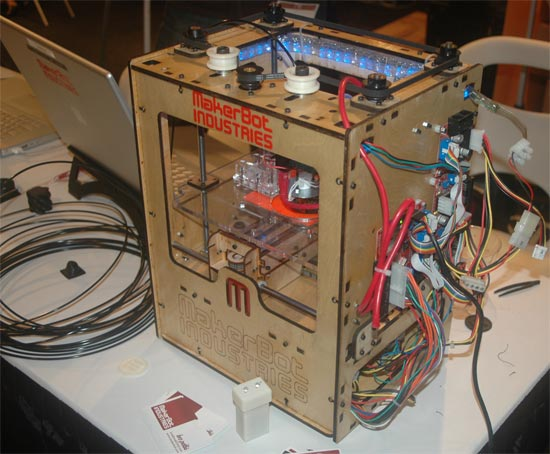
\includegraphics[width=.4\linewidth]{images/makerbot}&
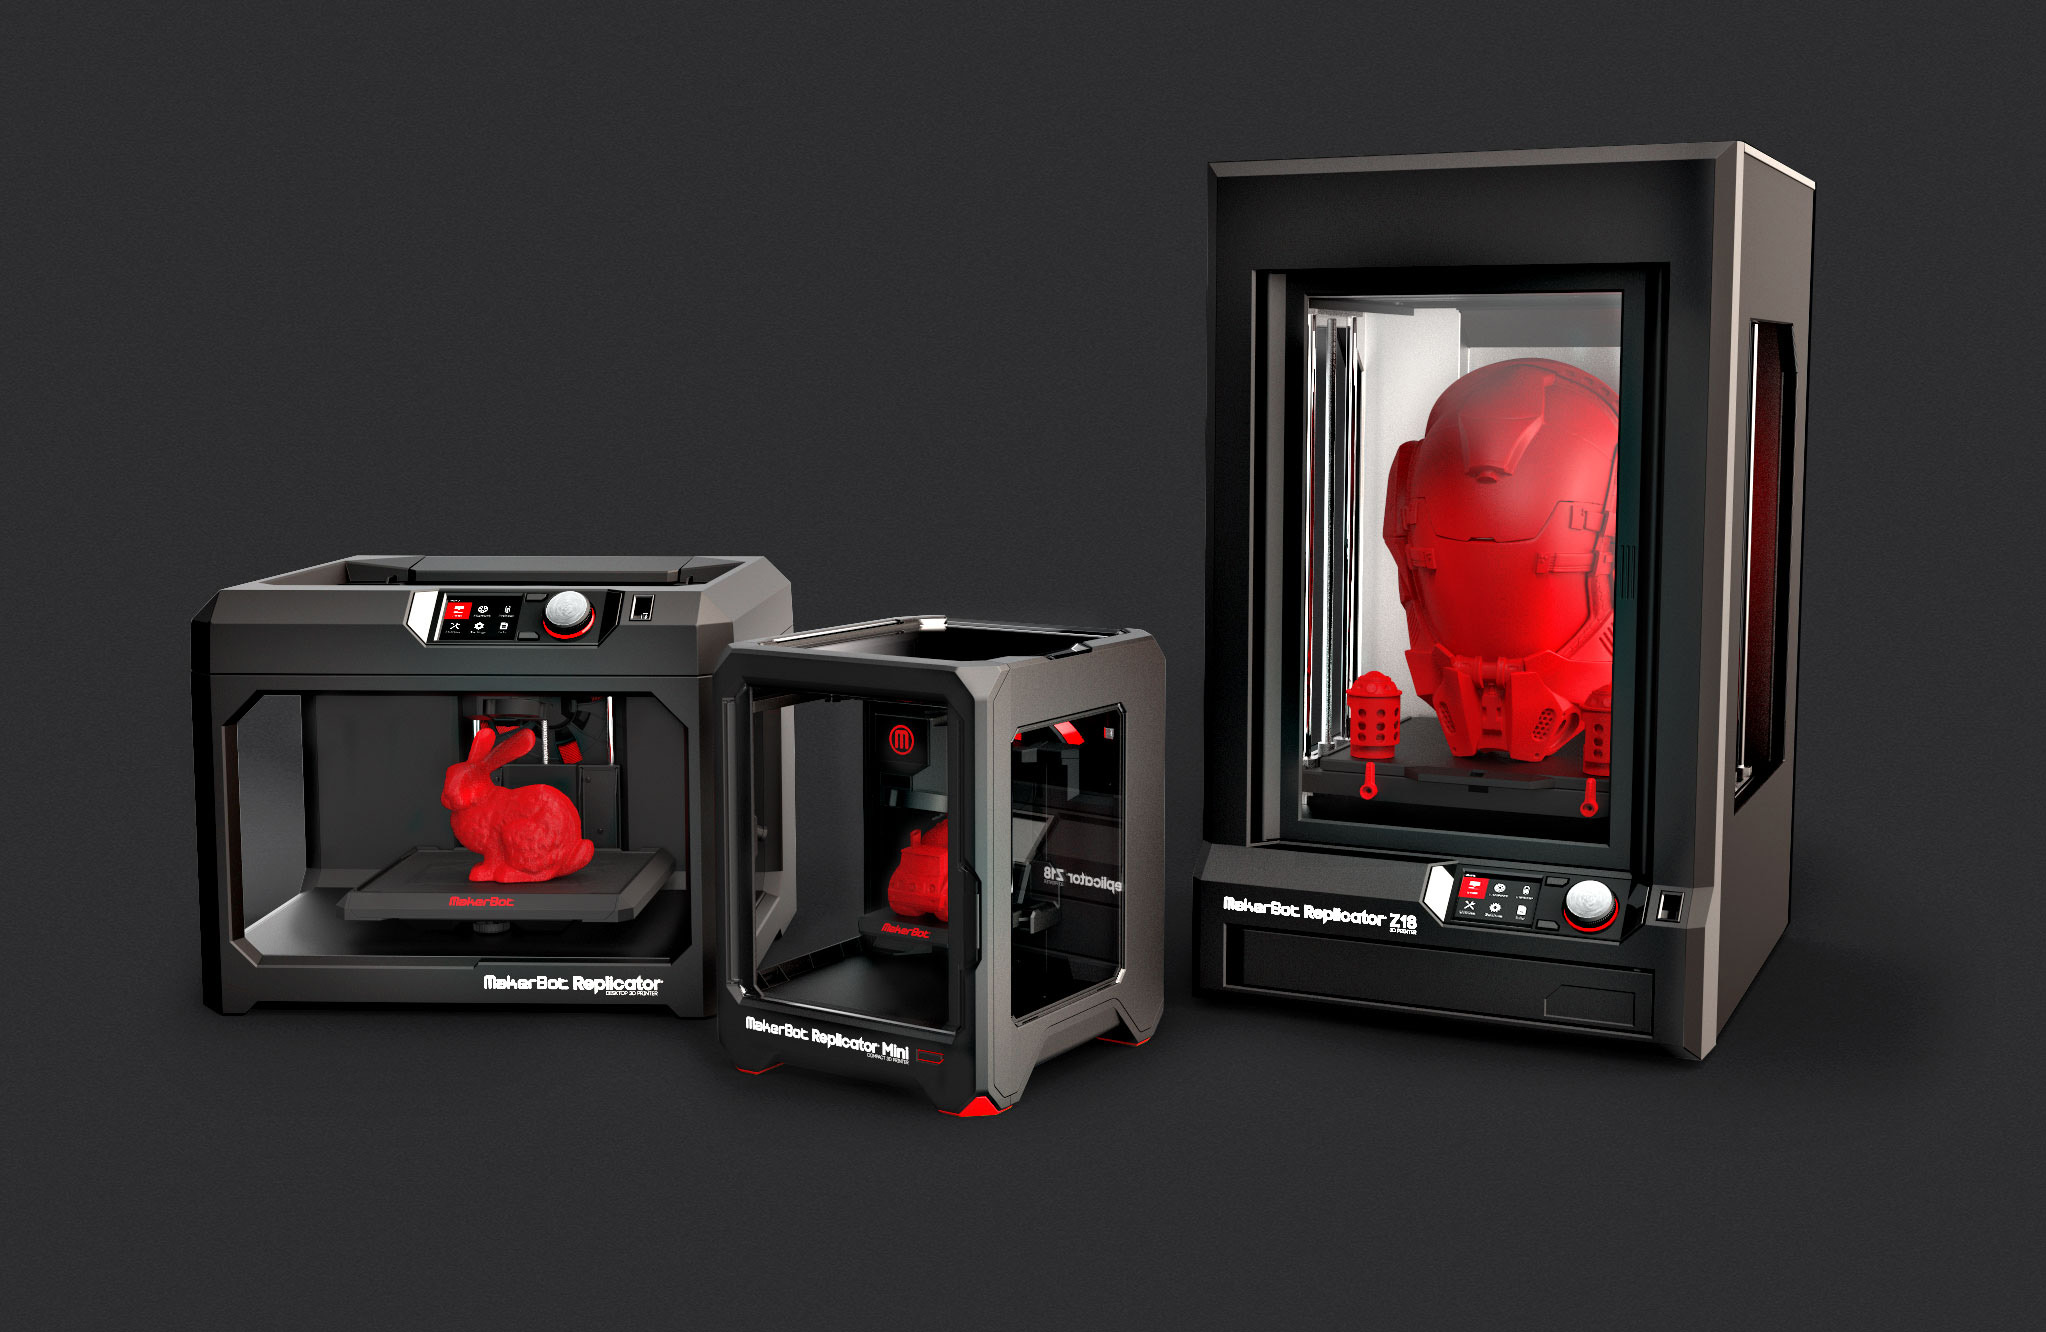
\includegraphics[width=.5\linewidth]{images/MB05_REP_Group}
\end{array}$
\end{center}
\caption{Left: One of the first popular desktop 3D printers, the MakerBot
``Cupcake CNC'', released in 2009. Right: The latest group of MakerBot models,
released at the Consumer Electronics Showcase in January 2014.}
\label{makerbot}
\end{figure}

Although printing out dozens of army men or barnyard animal figurines may be
satisfying for a time, and indeed speaks to the compelling nature of 3D
printing, it seems fair to say that children do not learn much about 3D modeling
from a ``download and print'' paradigm. Herein lies the crux of the problem - 3D
printing offers a wonderfully rich new platform for design, creativity, and
exploration, but neither the 3D printer manufacturers nor the companies who
produce the software necessary to author files suitable for 3D printing have
made accessibility for novices a priority. This is where our journey begins:
the desire to democratize 3D printing in a way that empowers newcomers,
particularly youngsters, in designing their own objects for 3D printing;
engaging them in such a way that intuitively introduces many of the core
concepts of 3D modeling, while helping to solidify cognitive processes around
spatial reasoning and 2D/3D translations, by building a set of devices that act
as a new genus amongst an ecosystem of next-generation digital fabrication
interfaces.

How, then, did we arrive at the term ``embodied fabrication'' to describe this
new genus? The simple answer, at the risk of over-extending the genealogical
metaphor, is that we selected what we deemed to be the best, most relevant
traits from a number of related areas (computer science, cognitive science,
developmental psychology, pedagogical theory, and digital fabrication
technology, amongst others) and attempted to splice them together in such a way
as to meaningfully address the issues with 3D printing outlined above. 

We derive the term ``embodied'' from cognitive science, and the fairly recent
advances in an area known as ``embodied cognition''. Embodied cognition posits
that our physical bodies and their interactions with the world are more closely
bound to our cognitive processes than previously thought. Evidence from research
in this area (discussed more thoroughly in Chapter 3 on related work) points to
cognitive benefits in basic arithmetic, ratios, proportions, and spatial
reasoning - all of which are useful (if not essential) tools in 3D modeling,
simply by involving the body more closely in the learning process.
This evidence, combined with the simple intuition that learning the skill of
3-dimensional modeling ought to be done in 3-dimensions as much as possible and
not solely on a 2-dimensional screen, provided the impetus for us to look toward
a physical solution that involves the body more than a typical piece
of software.

Physical, or ``tangible'' user interfaces are nothing new; wooden blocks have
been a part of children's education in a pedagogical sense since the beginning
of kindergarten over 150 years ago\cite{froebel}. Montessori ``manipulatives''
developed in the early part of last century inspired some of the first attempts
at creating physical, computationally-enhanced construction kits for children in
the 1980's\cite{Resnick:1998:DMN:274644.274684}. Tangible user interfaces, or
TUIs have been a growing part of human-computer interaction in a formal way
since Hiroshi Ishii's work on ``tangible
bits''\cite{Ishii:1997:TBT:258549.258715} in the mid 1990's, and of course the
influence of icons such as Doug Engelbart\cite{engelbart1968research} - one
might argue the mouse was the first ``embodied'' peripheral for a computer, in
the 1960's - and Mark Weiser\cite{weiser1991computer} (who presaged many of the
devices we take for granted today) as well as many others, should not be
overlooked - we give a more detailed account of this lineage when discussing
related work. For us, the longevity, breadth of applications, and numerous
achievements of mediating human-computer interaction though different physical
interfaces further suggests that a tangible user interface, coupled with the
proper software is more than capable of providing an accessible and embodied
foundation for our work.

Taking design principles from the lexicon of tangible user interfaces, adapting
them to better fit an embodied cognition world-view, and focusing on enabling 3D
modeling specifically for 3D printers, we designed and built a suite of
functional prototype devices for an embodied mode of digital fabrication; hence
the title of our work. To this end, we present a class of tangible user
interfaces designed to scaffold a child's ability to design, explore, and play
in three dimensions, with a particular focus on enabling original output for 3D
printing. We present three prototype devices (called UCube, SnapCAD,
and PopCAD) as well as piece of companion software that translates the physical
actions performed on the devices into screen-based content in real-time.

To give a brief preview of our creations; with their hands, users manipulate a
device to specify points (as coordinates in 3-space) that simultaneously display
as active dots against a ghosted 3D grid in real-time on a computer. The
software on the computer allows for certain modeling operations on this set of
input points (e.g., taking the convex hull, making a path through space),
exporting shapes to stereolithography (.STL) format with the click of a button,
the preferred format for 3D printers, as well as other functionality that we
explore more thoroughly in the next chapter.

We propose that these designs form a novel class of embodied input devices aimed
at enabling novice output for digital fabrication machines. Over three separate
user studies with 11 to 18 year olds, we investigate the ability for children to use
our devices to model a given shape (with and without the companion software) and
to match configurations on our device to a printed 3-dimensional object (without
the aid of the software). In our last study we compare two of our devices over a
multi-session study, while also administering a set of spatial reasoning tasks
as a pre and post test. We video record the subjects (with parental consent)
and analyze the gesture and speech expressions the participants make when
explaining a modeling strategy to reproduce a given object.

Through our studies, we show evidence that our suite of devices can be used
effectively by young adolescents with very minimal instruction, that a wide
variety of shapes can be recreated by the majority of subjects who used our
devices, that spatial test scores and modeling performance tends to improve over
multiple sessions with our devices, and that the kinds of gestures produced
while explaining modeling strategy correlates to modeling success on our
devices, a finding which supports prior research on gesture analysis by other
authors.

By providing a feedback loop between the bodily interaction with
tangible interfaces and the observed changes in real-time on a computer screen,
this body of work presents strong new motives for the inclusion of embodied
cognition in tangible interface design, while tackling the lack of appropriate
tools for novices to create for 3D printers, and evaluating the efficacy of our
devices as modeling tools and as devices for strengthening spatial reasoning and
cognition. We continue in Chapter 2 to present our prototype devices and the
software they operate with, explaining the evolution of our design choices as
well as the technical details behind their operation. Chapter 3 details the lineage
of related work, hinted at somewhat in this introduction, drawing connections
between the childhood developmental theories and conceptions of space developed
by Piaget and refined by Papert, the notions of cognitive development and
embodied mathematics discussed by Lakoff and Nu\~nez, the democratization of
digital fabrication technologies discussed by Gershenfeld and Lipson, and the
previous adaptation of these achievements into computer science. Chapter 4 is
devoted to the evaluation of our work, presenting three user studies, their
procedures and results. Chapter 5 delves deeper into the discussions which
surround the observations from our studies, comparing them with prior research,
and against each other. Finally, Chapter 6 provides a vision for immediate
future work on our devices, a more expansive vision of the possibilities
inherent in embodied fabrication, and ends with our concluding thoughts.



% The work presented here draws on the stages of childhood developmental theories
% and conception of space developed by Piaget and refined by Papert, notions of
% cognitive development and embodied mathematics discussed by Lakoff and Nu\~nez,
% the democratization of digital fabrication technologies discussed by Gershenfeld
% and Lipson, and the previous adaptation of these achievements into computer
% science.
























%old intro
% Digital fabrication technologies are increasingly finding their way into
% educational spaces of all shapes and sizes. These new technologies 
% (3D printers, laser cutters, etc.) afford opportunities for exploring these new
% ways of `making' and how they may change the way we learn, explore, and play.
% Although there is much excitement surrounding the `maker movement' - and 3D
% printing in particular - there has been little examination of how to introduce
% a younger audience to 3D printing in an empowering way.
% This proposal argues that tangible interfaces - as opposed to 2D screen-based
% media - can be designed not only to support spatial reasoning and mathematical
% intuitions in children by engaging them in exploratory modeling and play, but
% that these interfaces can act as a democratizing force by enabling children to
% create physical objects with digital fabrication devices.
% The proposed work presents a series of novel tangible input devices for
% enhancing mathematical and spatial reasoning in kids with a focus on generating
% output for 3D printing. We discuss related work, the status of the proposed
% work, additional improvements to be made, a timeline for completion,
% and a discussion of risks, limitations, and outcomes inherent in the proposal.
% 
% 
% %from proposal
% A number of computer scientists, technologists, and educators have declared that
% the era of personal fabrication is upon
% us\cite{anderson2012makers}\cite{Gershenfeld:2007:FCR:1211574}. New devices
% aimed at increasing the ability of the individual to physically manufacture
% their own ideas are being released at breakneck speed. The cultural and
% technological shifts caused by this change are taking many forms, yet few
% technologies associated with the `maker' movement have received as much
% attention as 3D printing - the ability (by various means) to digitally design
% and then print out physical 3-dimensional objects. Media outlets from
% Forbes\cite{forbes} to The Economist\cite{economist} have extolled the
% disruptive and democratizing possibilities that 3D printing offers - at least as
% it affects the traditional manufacturing supply chain. Less examined has been
% how to introduce novices, specifically pre-teens and early adolescents, to 3D
% printing - and perhaps more importantly - discussing what (and how) they might
% learn by being exposed to it.
% While the variety of desktop 3D printers continues to increase and the cost of
% adding a `fab lab' of digitally-based manufacturing tools in the home or
% classroom steadily declines, the types of interfaces by which children can
% easily and intuitively design and explore the capabilities of 3D printers still
% remains a barren landscape consisting primarily of software-only solutions. It
% is this landscape that we are interested in seeding, following the best
% practices in computational and cognitive science with particular attention to
% children-centered design.




% \section{A Brief Overview of this Thesis}
% 
% \section{Motivations}

\chapter{Prototype Systems}
\label{prototypes}

Over the past several years we have been working on the creation of a family of
child-friendly tangible user interfaces that would serve as input devices for
exploring 3D modeling and digital fabrication in an ``embodied'' fashion. As
discussed in the first chapter, the motivations behind this work are
thematically diverse, but can be distilled into an attempt to create a more
intuitive, body-centric way for novices to design for 3D printing while also
strengthening the user's sense of spatial translation from 3D to 2D (screen
based) representations. To this end, we have created three prototypes:
the UCube, an initial proof-of-concept device using simple components, SnapCAD,
a more expressive and capable iteration of the UCube relying on magnetized LED
circuit boards, and PopCAD - a paper-based interface addressing several of the
cost and portability concerns raised by SnapCAD. These systems all communicate
with versions of a companion software program running on desktop computer. This
chapter describes (in chronological order) the development of these three
systems, the software that interfaces with them, the motivations behind their
design, and the technical work involved in their creation.

\section{UCube}

The UCube represents our first attempt to create a cooperative system of
hardware and software that encapsulated and combined our beliefs about embodied
cognition and the importance of accessible digital fabrication. The idea for the
UCube originally came from the attempt to create a ``3D Geoboard''.
\ref{fig:geoboard} shows a rudimentary 2D geoboard consisting of a 3x3 grid
of nails stuck into a wooden block. Simple geometries, such as the triangle shown
in the referenced image, can be made by stretching rubber bands around some
number of ``pegs''. The geoboard invites a kind of tangible, exploratory, and
embodied play that (as we discuss in Chapter 3) promotes children's learning in
powerful ways. The initial design goal was to capture the ``gestalt'' of
the traditional 2-dimensional geoboard and extend it - into 3-dimensions, and with a
computationally-enhanced interface that could translate physical manipulations
on a device into a software program that could display the actions performed on
the geoboard in a ``meaningful'' way - that is, in a way that could potentially
extend spatial reasoning abilities between the 3D representations created on
the device and the 2D, screen-based images displayed on the computer screen.

\begin{figure}[ht]
\begin{center}$
\begin{array}{cc}
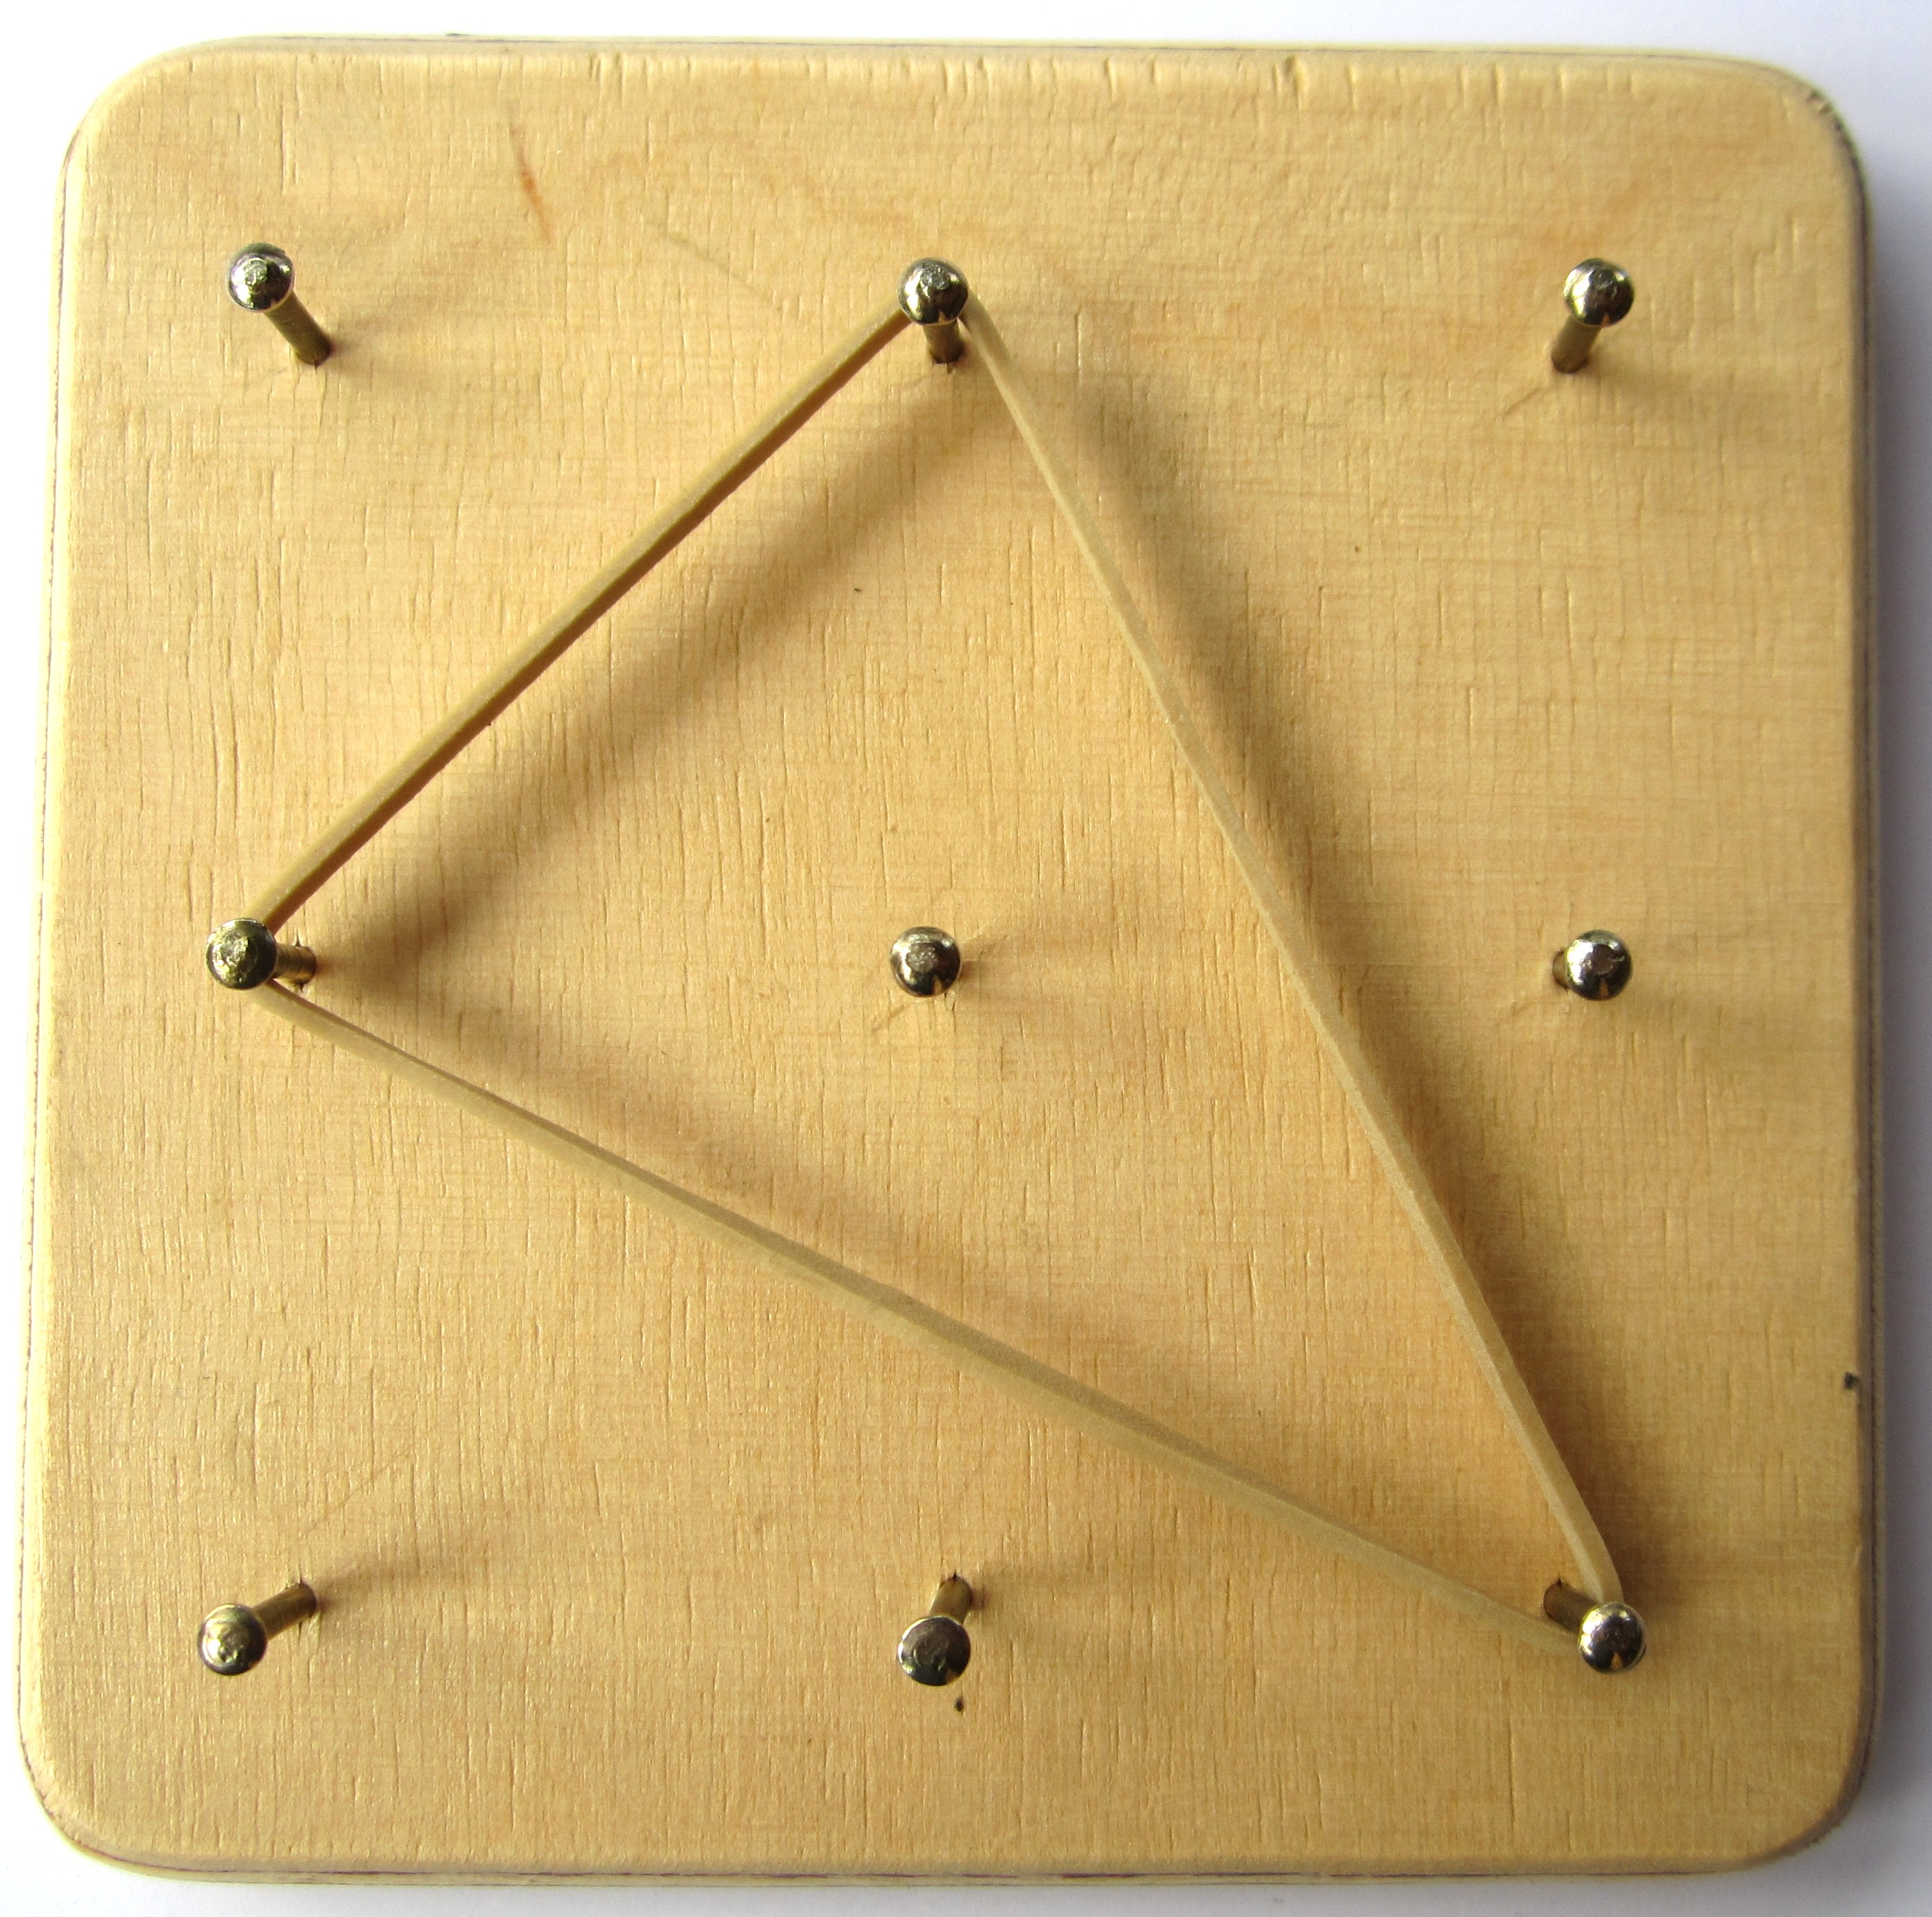
\includegraphics[width=.5\linewidth]{images/Geoboard}
\end{array}$
\end{center}
\caption{A simple 3x3 geoboard, with a rubber band stretched around several
pegs, forming a triangle.}
\label{fig:geoboard}
\end{figure}

The UCube (as seen on the left in \ref{fig:ucube1}) is the initial result of
this goal. The physical interface consists of a set of vertical ``towers'' that
are placed (and optionally re-placed) onto a grid of 4x4 evenly spaced nodes or
sockets, which act somewhat like the nails in the 2D geoboard. The towers
themselves contain four switches placed vertically along the tower, creating a
potential for 64 (4x4x4) distinct points to be activated. The towers are
``plugged in'' when placed into one of the 16 socket nodes, connecting them to
the underlying circuitry responsible for providing power to the towers and
relaying the state of each of the switches to the computer, via an Arduino
Mega\cite{ArduinoMega} microcontroller. Thus, when a tower is placed in a
specific node on the board and a switch is flipped on, a particular (x,y,z)
coordinate in three-dimensional space is activated and sent to a piece of
software on the computer. An abstracted illustration of the hardware system is
seen on the right in \ref{fig:ucube1_schematic}.

\begin{figure}[!ht]
\begin{center}$
\begin{array}{cc}
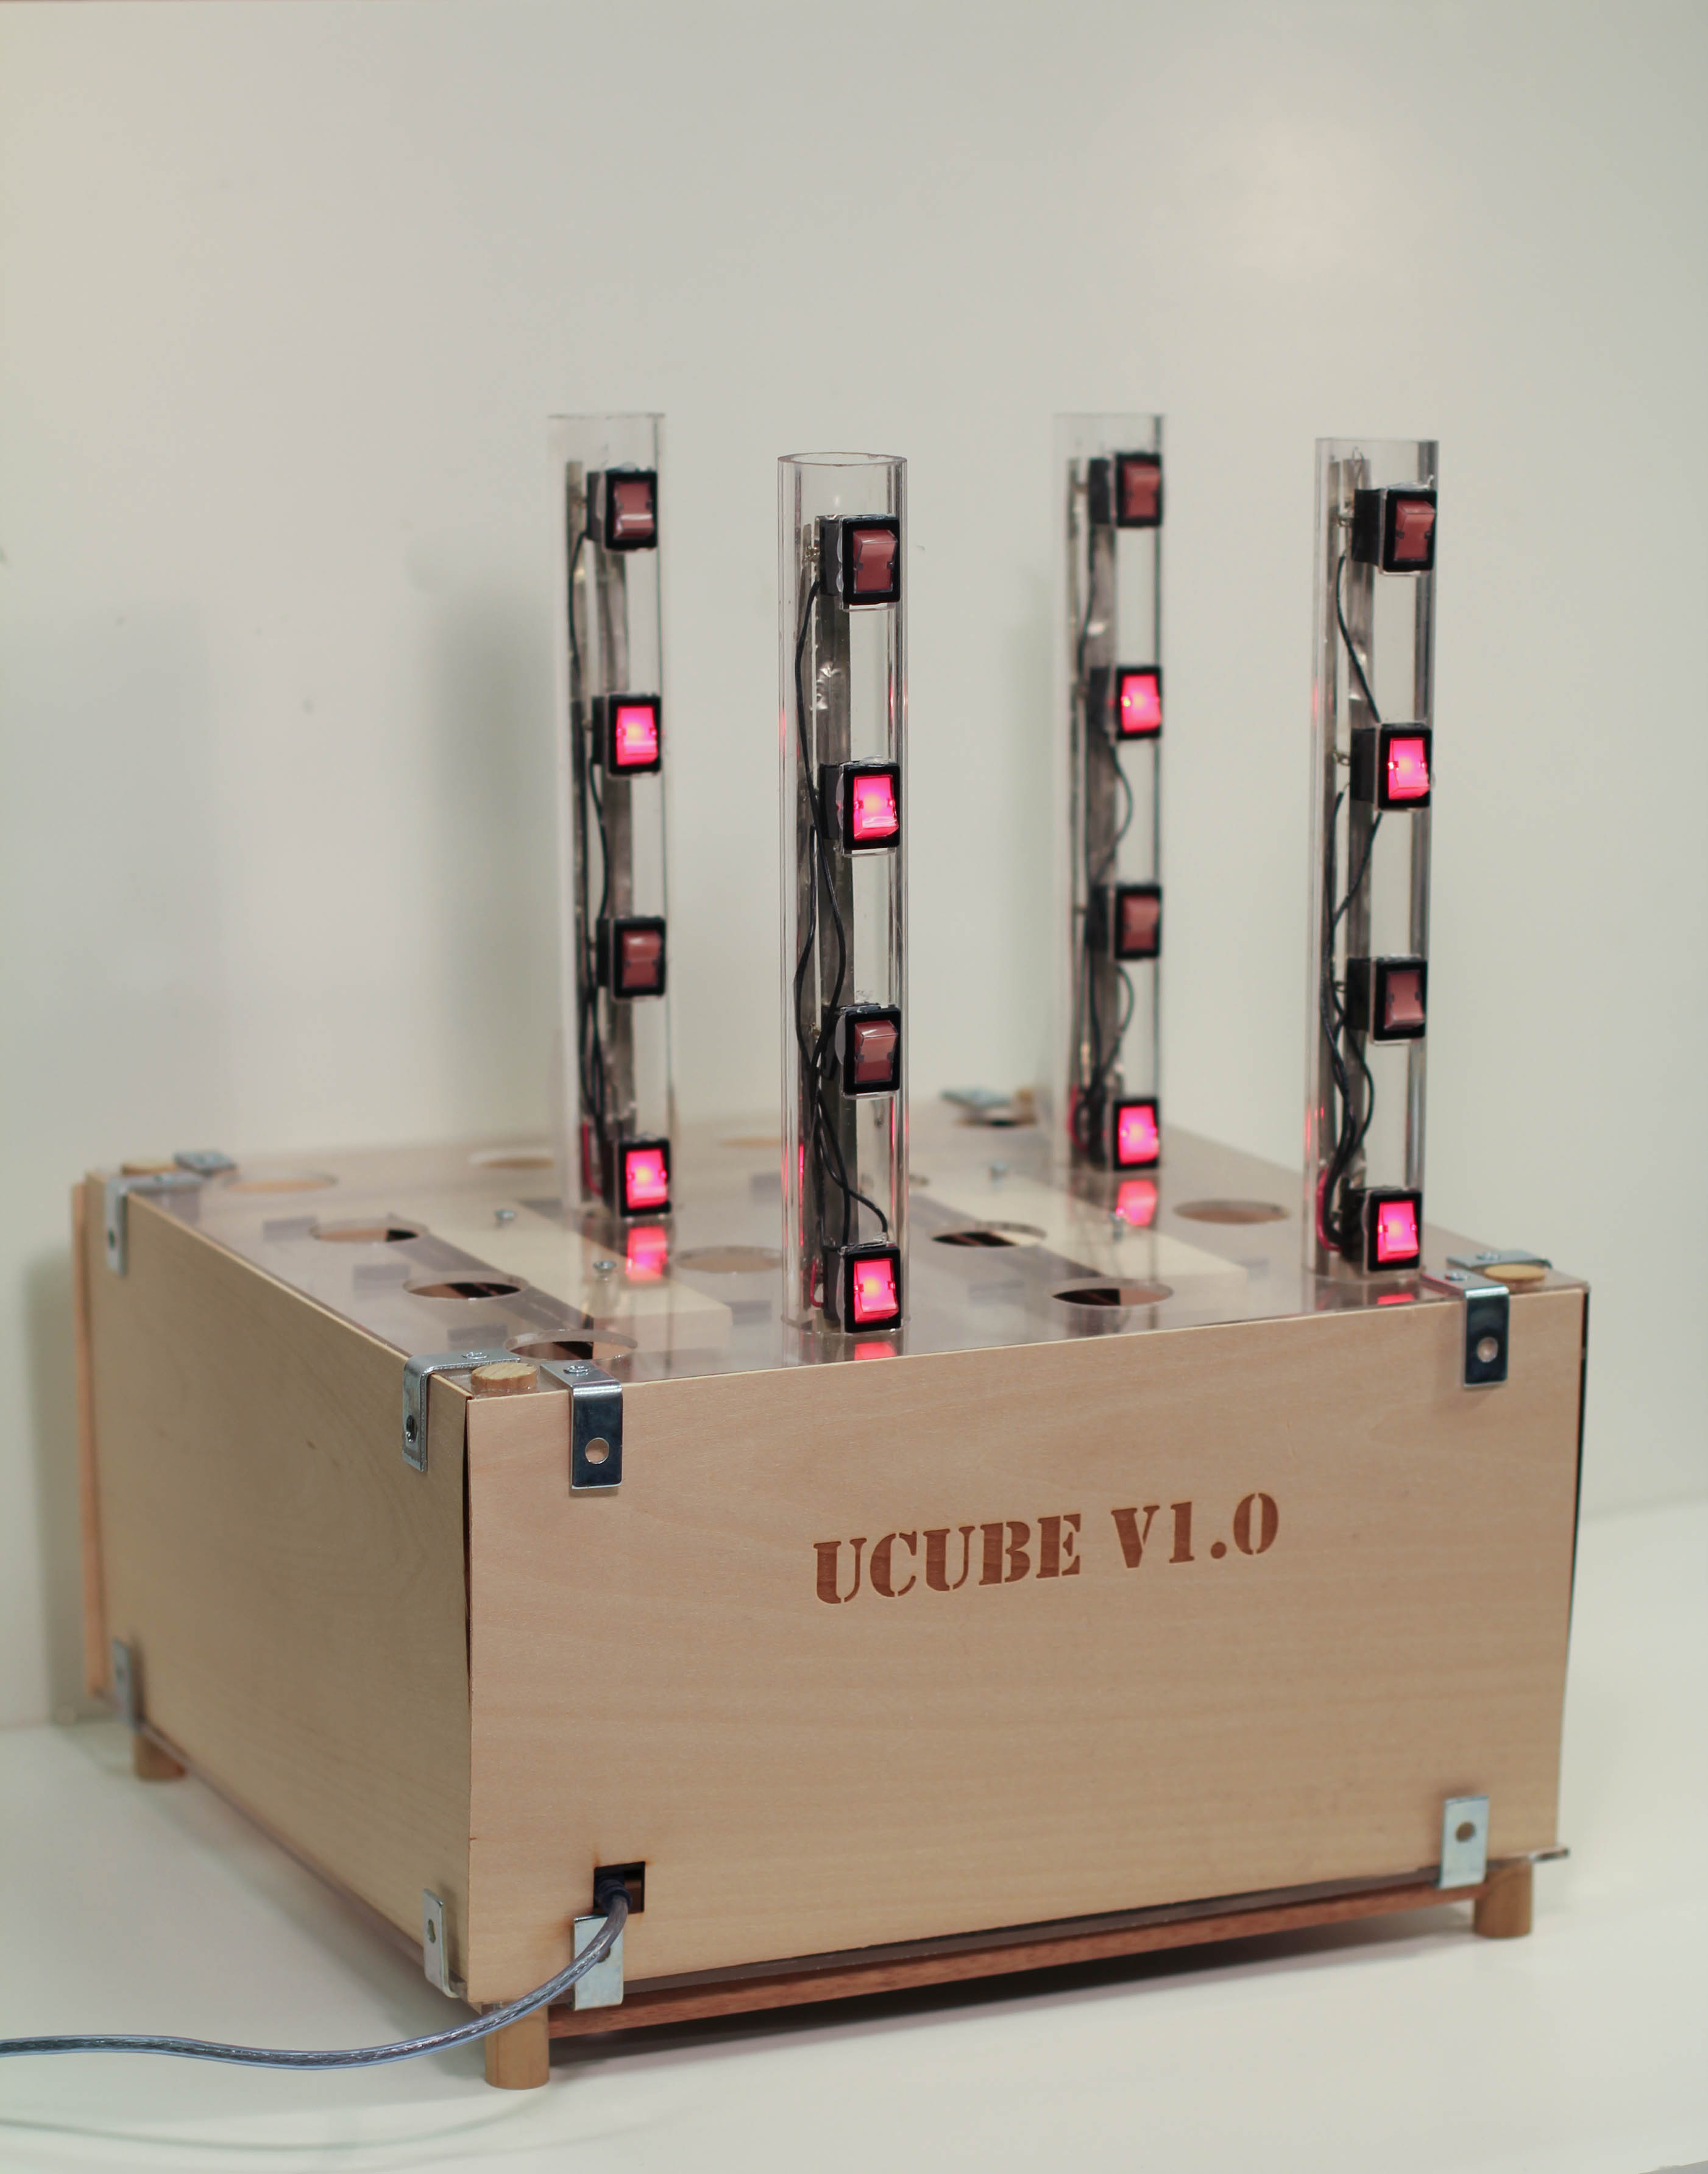
\includegraphics[height=3in]{images/UCube-3}&
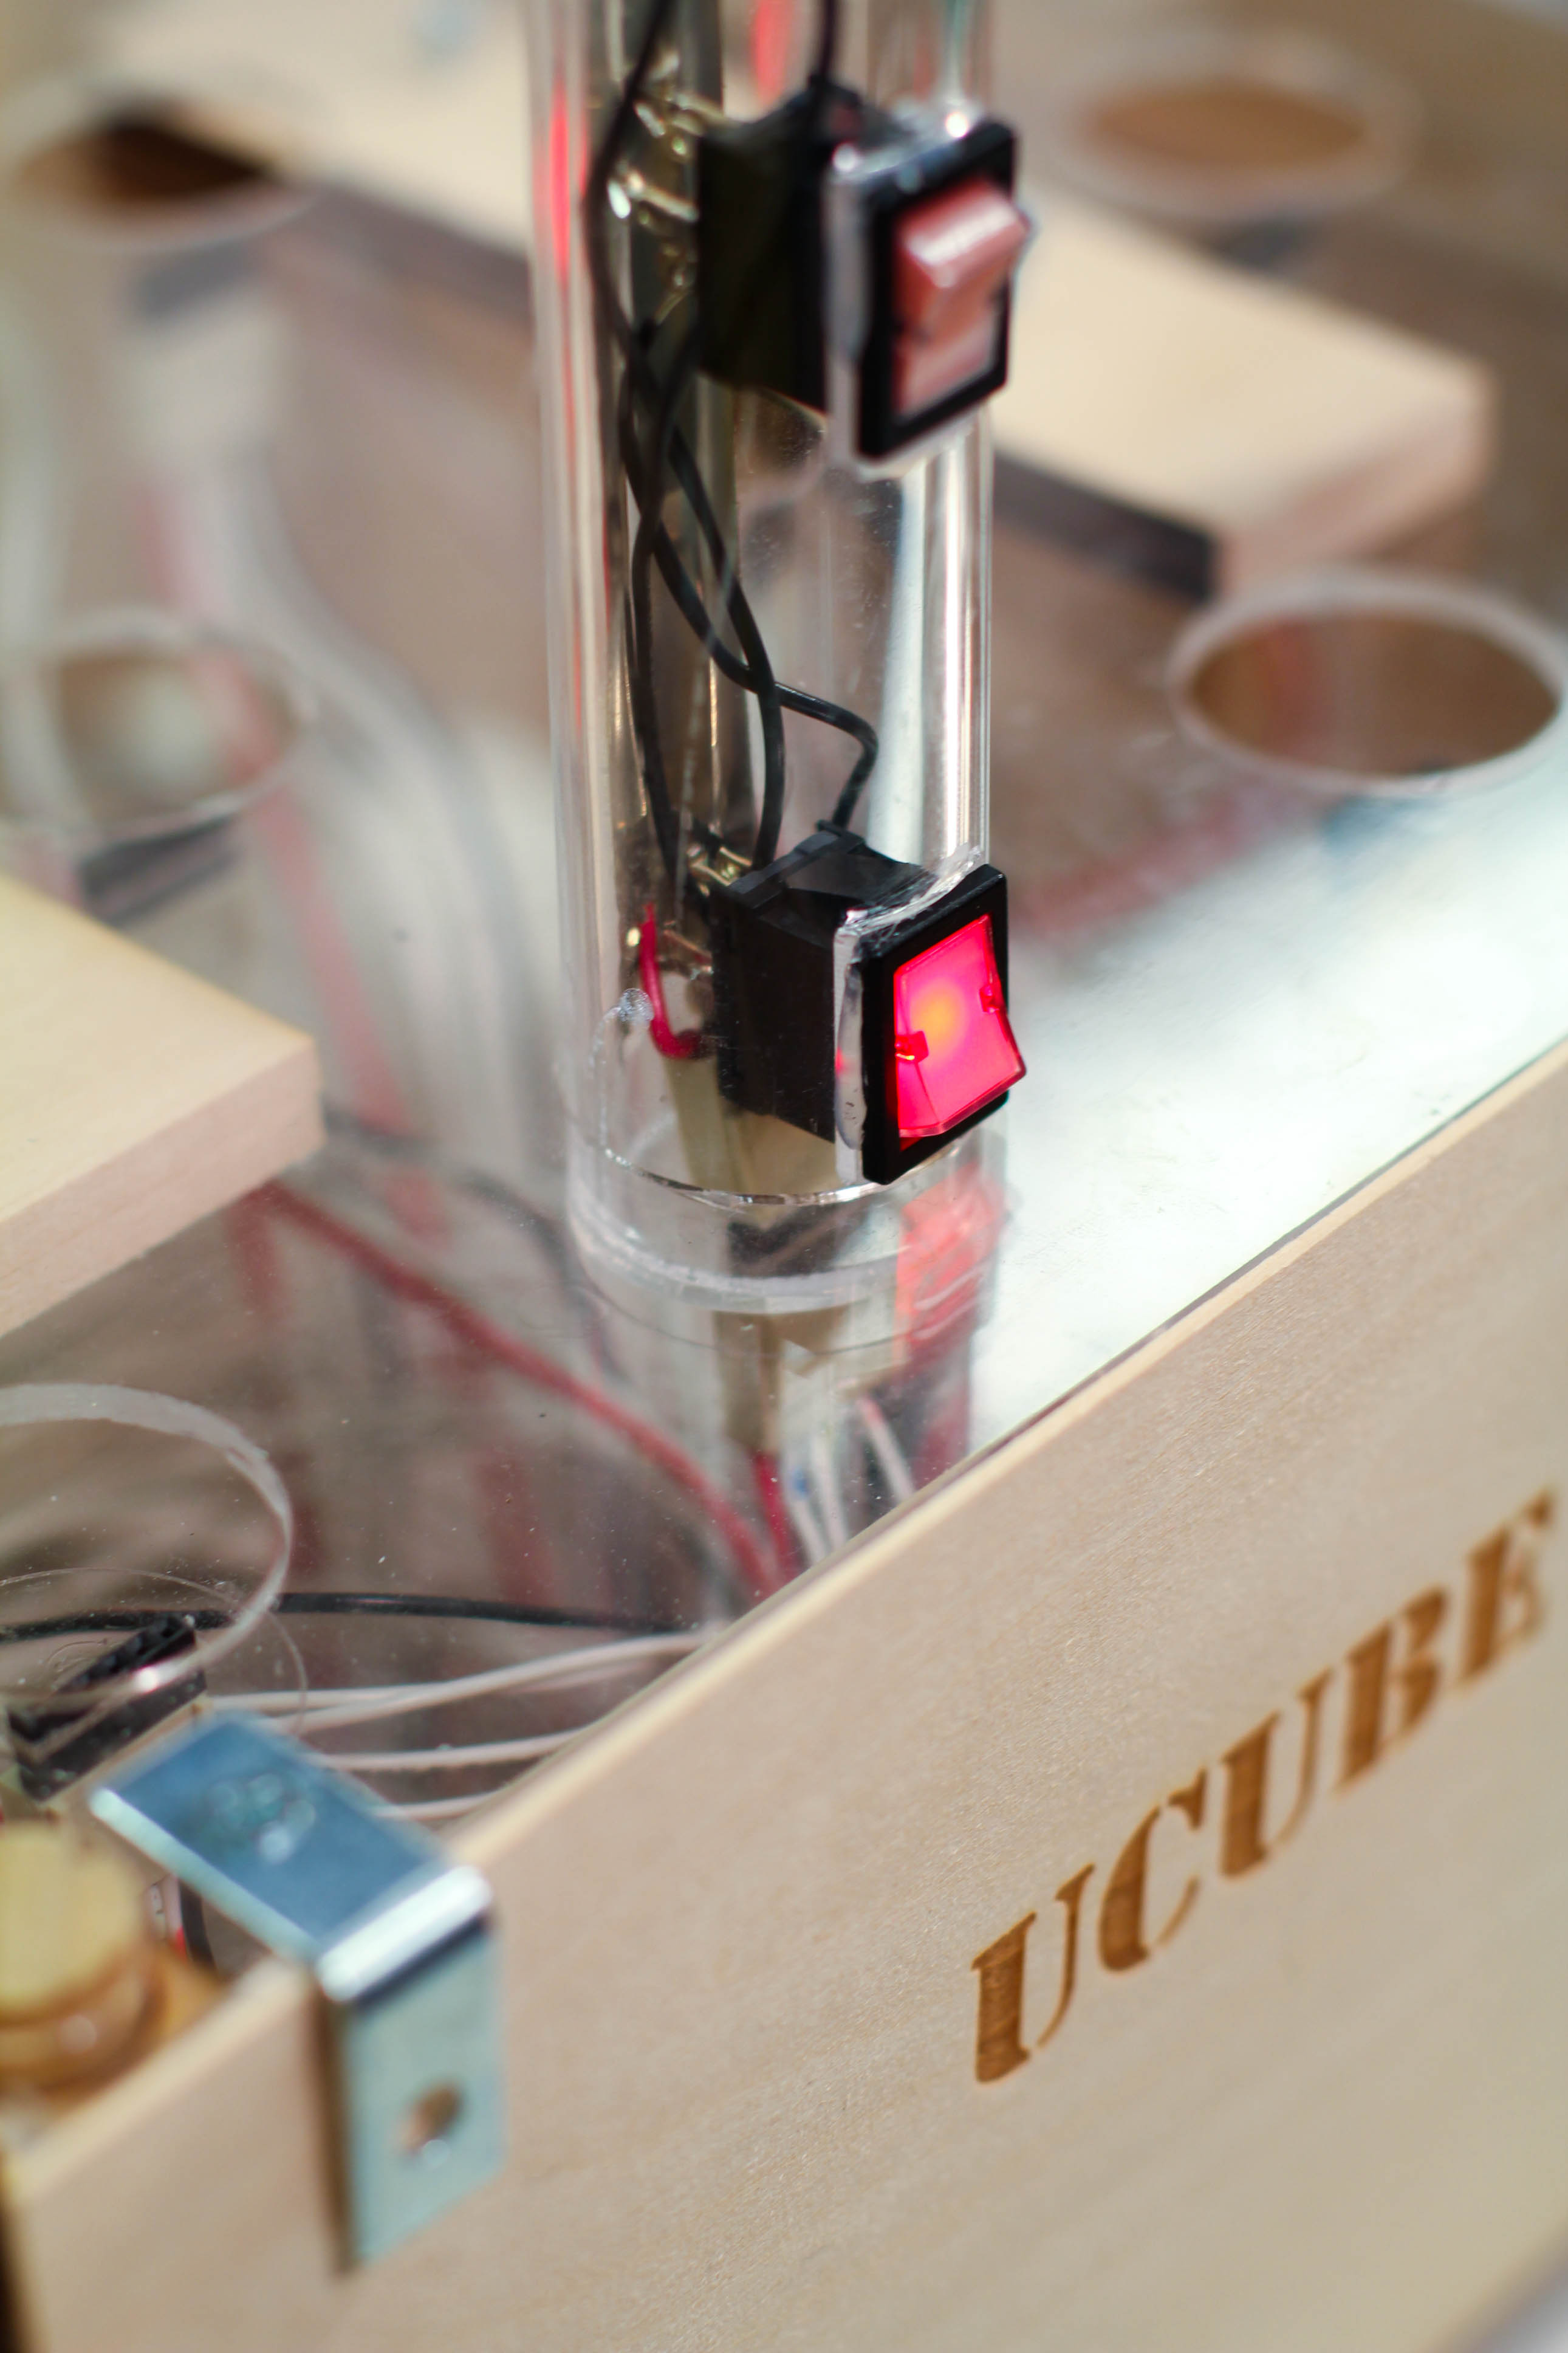
\includegraphics[height=3in]{images/UCube-4}
\end{array}$
\end{center}
\caption{Left: The UCube device, with four towers and eight lit switches,
representing (in one instance) the eight vertices of a cube. Right: A detail
view of one of the towers placed into the UCube modeling board with the bottom
switch lit.}
\label{fig:ucube1}
\end{figure}

Figure \ref{fig:ucube1} shows two views of the UCube interface. The picture on
the left shows the device, with four towers placed in an evenly spaced square,
with one ``board unit'' separating each tower. The lowest and third-lowest
switches on each tower are lit, marking eight active points. Thus we have eight
active points, spaced evenly in such a way to describe a cube of 2
``board-units'' in length if we were to take the convex hull of those points.
The photo on the right gives a detailed view of the UCube hardware. A tower has
been plugged into the board and its bottom-most switch turned to the ``on''
position. 


The UCube software (discussed more thoroughly later in the chapter)
takes the incoming coordinate data from the microcontroller and translates it
into a real-time visualization on screen. The graphical user interface centers
around a ``ghosted'' grid of all the potential points, with the active points
being highlighted. In the first version of the software, the interface also
provides a set of operations that can be performed on the set of active points
in addition to normal scene manipulations like zoom and rotate. These functions
are explained more thoroughly in the software section later in the chapter, but
to give a brief list, include: taking the convex hull of the point set (as
imagined in \ref{fig:ucube1}), creating a sequential path or knot through the
active points, exporting the convex hull or knot to .STL format for 3D printing,
drawing a (non-printable) spline through the active points, saving and loading a
shape, and editing the vertices of a convex hull via a click-and-drag interface.



% from IDC 2011 paper
% As a first step in discussing the UCube's role in spatial design�and in
% discussing the broader issue of children's three-dimensional design�this section
% is devoted to a more thorough description of the UCube and its operation.
% To begin with an overview, then: the UCube system is the combination of two
% elements: the physical input device of ``towers'' placed on a board, and the
% companion display software. These two systems work together to take the embodied
% actions of the user and display corresponding points and shapes on the computer.
% A sense of the scale of the device can be inferred from \ref{fig:cubev2}, which
% shows a photograph of a middle-school student holding a newly-placed tower in
% the UCube platform while pointing simultaneously at the desktop computer screen
% beside it.
% This photograph�which we will also return to in the discussion of pilot testing
% in a later section�reflects the essential nature of interaction with the device:
% points are designated in a spatial region provided by the platform, and then
% represented in real time on the computer screen. Thus, the UCube promotes an
% attention to the correspondence between the selected spatial points above the
% platform and the (more abstract) representation on the computer screen.

\subsection{Technical Implementation} 
The physical system for our first UCube prototype, as outlined earlier, consists
of a platform with a four-by-four grid of potential sites, each of which can
hold one tower with four switches, thus describing a 4x4x4 array of 64 potential
points. The platform structure consists of three different horizontal
``layers''. The top (or upper surface) layer is a clear 1/4'' acrylic square,
into which a four-by-four grid of circular holes has been laser cut in such a
way that the towers fit snugly. This layer of clear acrylic acts as a brace to
hold the towers upright, helps guide the pins from the tower into alignment with
the socket into which they must be placed, and ensures that the towers
themselves are resistant to being knocked over.

The next layer down holds a set of headers, six per socket (one each for power
and ground, and four input lines, one for each switch), which allow the towers
to ``plug in'' and connect to the rest of the circuit. Wires from the headers go
down to the bottom layer, which holds the breadboarded circuit and Arduino Mega
microcontroller\cite{ArduinoMega}. The header wires connect directly to the
breadboard, where each switch circuit runs through a 10K$\Omega$ resistor, and
then to a digital input pin on the Arduino Mega. When plugged in, the Arduino is
able to communicate (via asynchronous serial communication) the set of active
switches (and corresponding coordinates) to the computer through a USB cable.
\ref{fig:ucube1_schematic} depicts a schematic diagram of the UCube hardware.

\begin{figure}[!ht]
\begin{center}$
\begin{array}{cc}
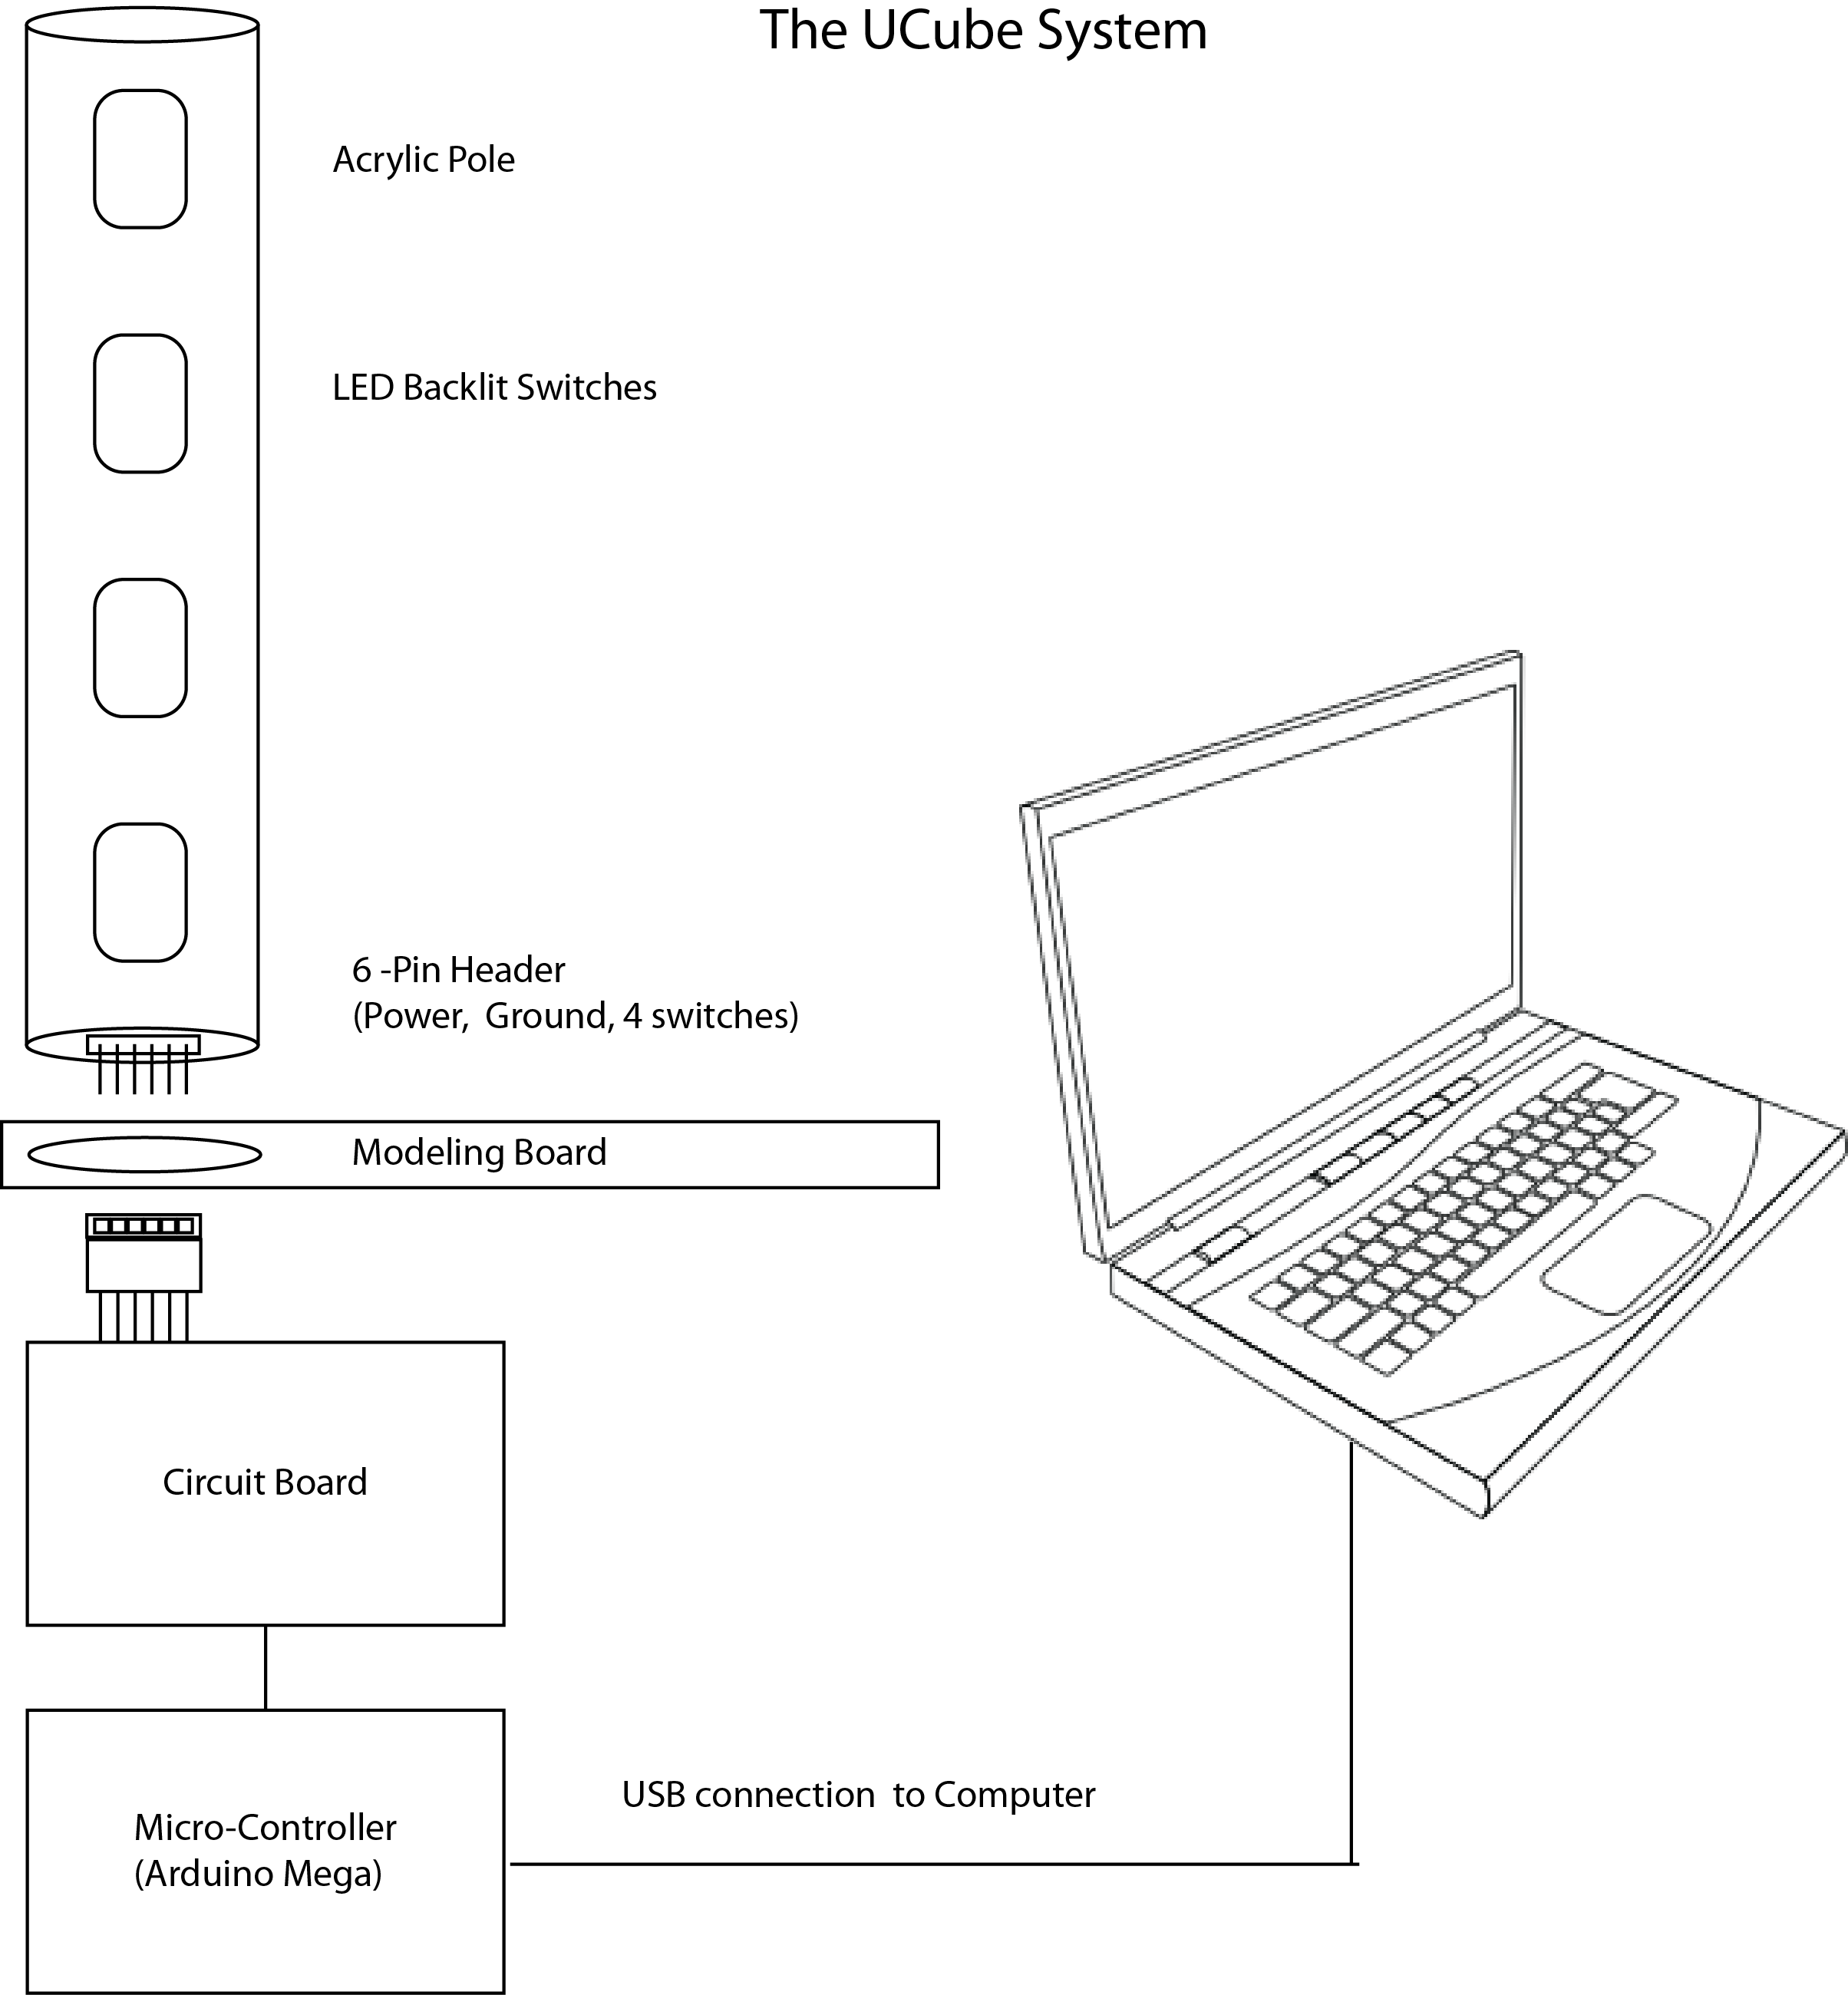
\includegraphics[width=.5\linewidth]{images/ucube_diagram}
\end{array}$
\end{center}
\caption{A schematic illustration of the UCube hardware.}
\label{fig:ucube1_schematic}
\end{figure}

The towers are made of transparent acrylic, cut from a 1'' diameter circular
tube. The towers were laser-cut in order to house the four switches and
corresponding circuitry elements. Four laser-cut rectangles are sized to allow
the back of each switch to be placed inside the tower while the faceplate
remains on the surface. The switched are backlit with in-built red LED's. Each
switch has a 270$\Omega$ current limiting resistor soldered between two of its
legs to protect the lighting element. Headers were soldered on to the power and
ground pins of the switch, and connect to a strip of conductive tape affixed to
the back on the inside of the tower (one can make this out somewhat in Figure
\ref{fig:ucube1}). The signal line from the switch (responsible for letting the
microcontroller know it has been switched) is soldered to a wire which reaches
down a six-pin header at the base of the tower. As the switches are LED-backlit
when active, it becomes more apparent which points are active as well as giving
a more accessible ``gestalt'' of the shapes being modeled. The luminosity also
allows for some potentially interesting applications in dimly-lit circumstances,
such as modeling constellations in a classroom or planetarium: in these
situations, the lights of the selected spatial points stand out especially
vividly.


\subsection{A Sample UCube Scenario}
As a sample scenario, imagine that we wish to create a triangular prism solid
employing the UCube. We can begin this process by selecting three points to form
a triangle; then, by placing two more towers and creating the same triangular
shape "shifted over" by two units (as seen on the left of \ref{fig:cubev1}) we
create the entire prism. Naturally, there might be many alternative pathways to
forming the same eventual shape: for example, we might begin by placing four (or
more) towers in the platform, and then experiment or fiddle with the chosen
lights to approach the eventual goal of creating our prism. Alternatively, we
might begin without any towers in the device at all: by placing our hands or
fingers above the device, roughly indicating where the prism should be, we might
then use our imagined locations as ``guides'', helping us to place the necessary
towers in the platform and select the correct lights for the vertices of the
prism.
In any event, having designed the prism using the UCube platform, and having
checked that it looks like the correct shape on the computer screen (as seen in
the center of \ref{fig:cubev1}), the final step is to export the shape into a
format suitable for 3D printer output. The UCube software, as noted earlier,
includes a feature for doing just this; and finally, we print out the prism, as
shown on the right in \ref{fig:cubev1}.

\begin{figure}[!ht]
\begin{center}$
\begin{array}{ccc}
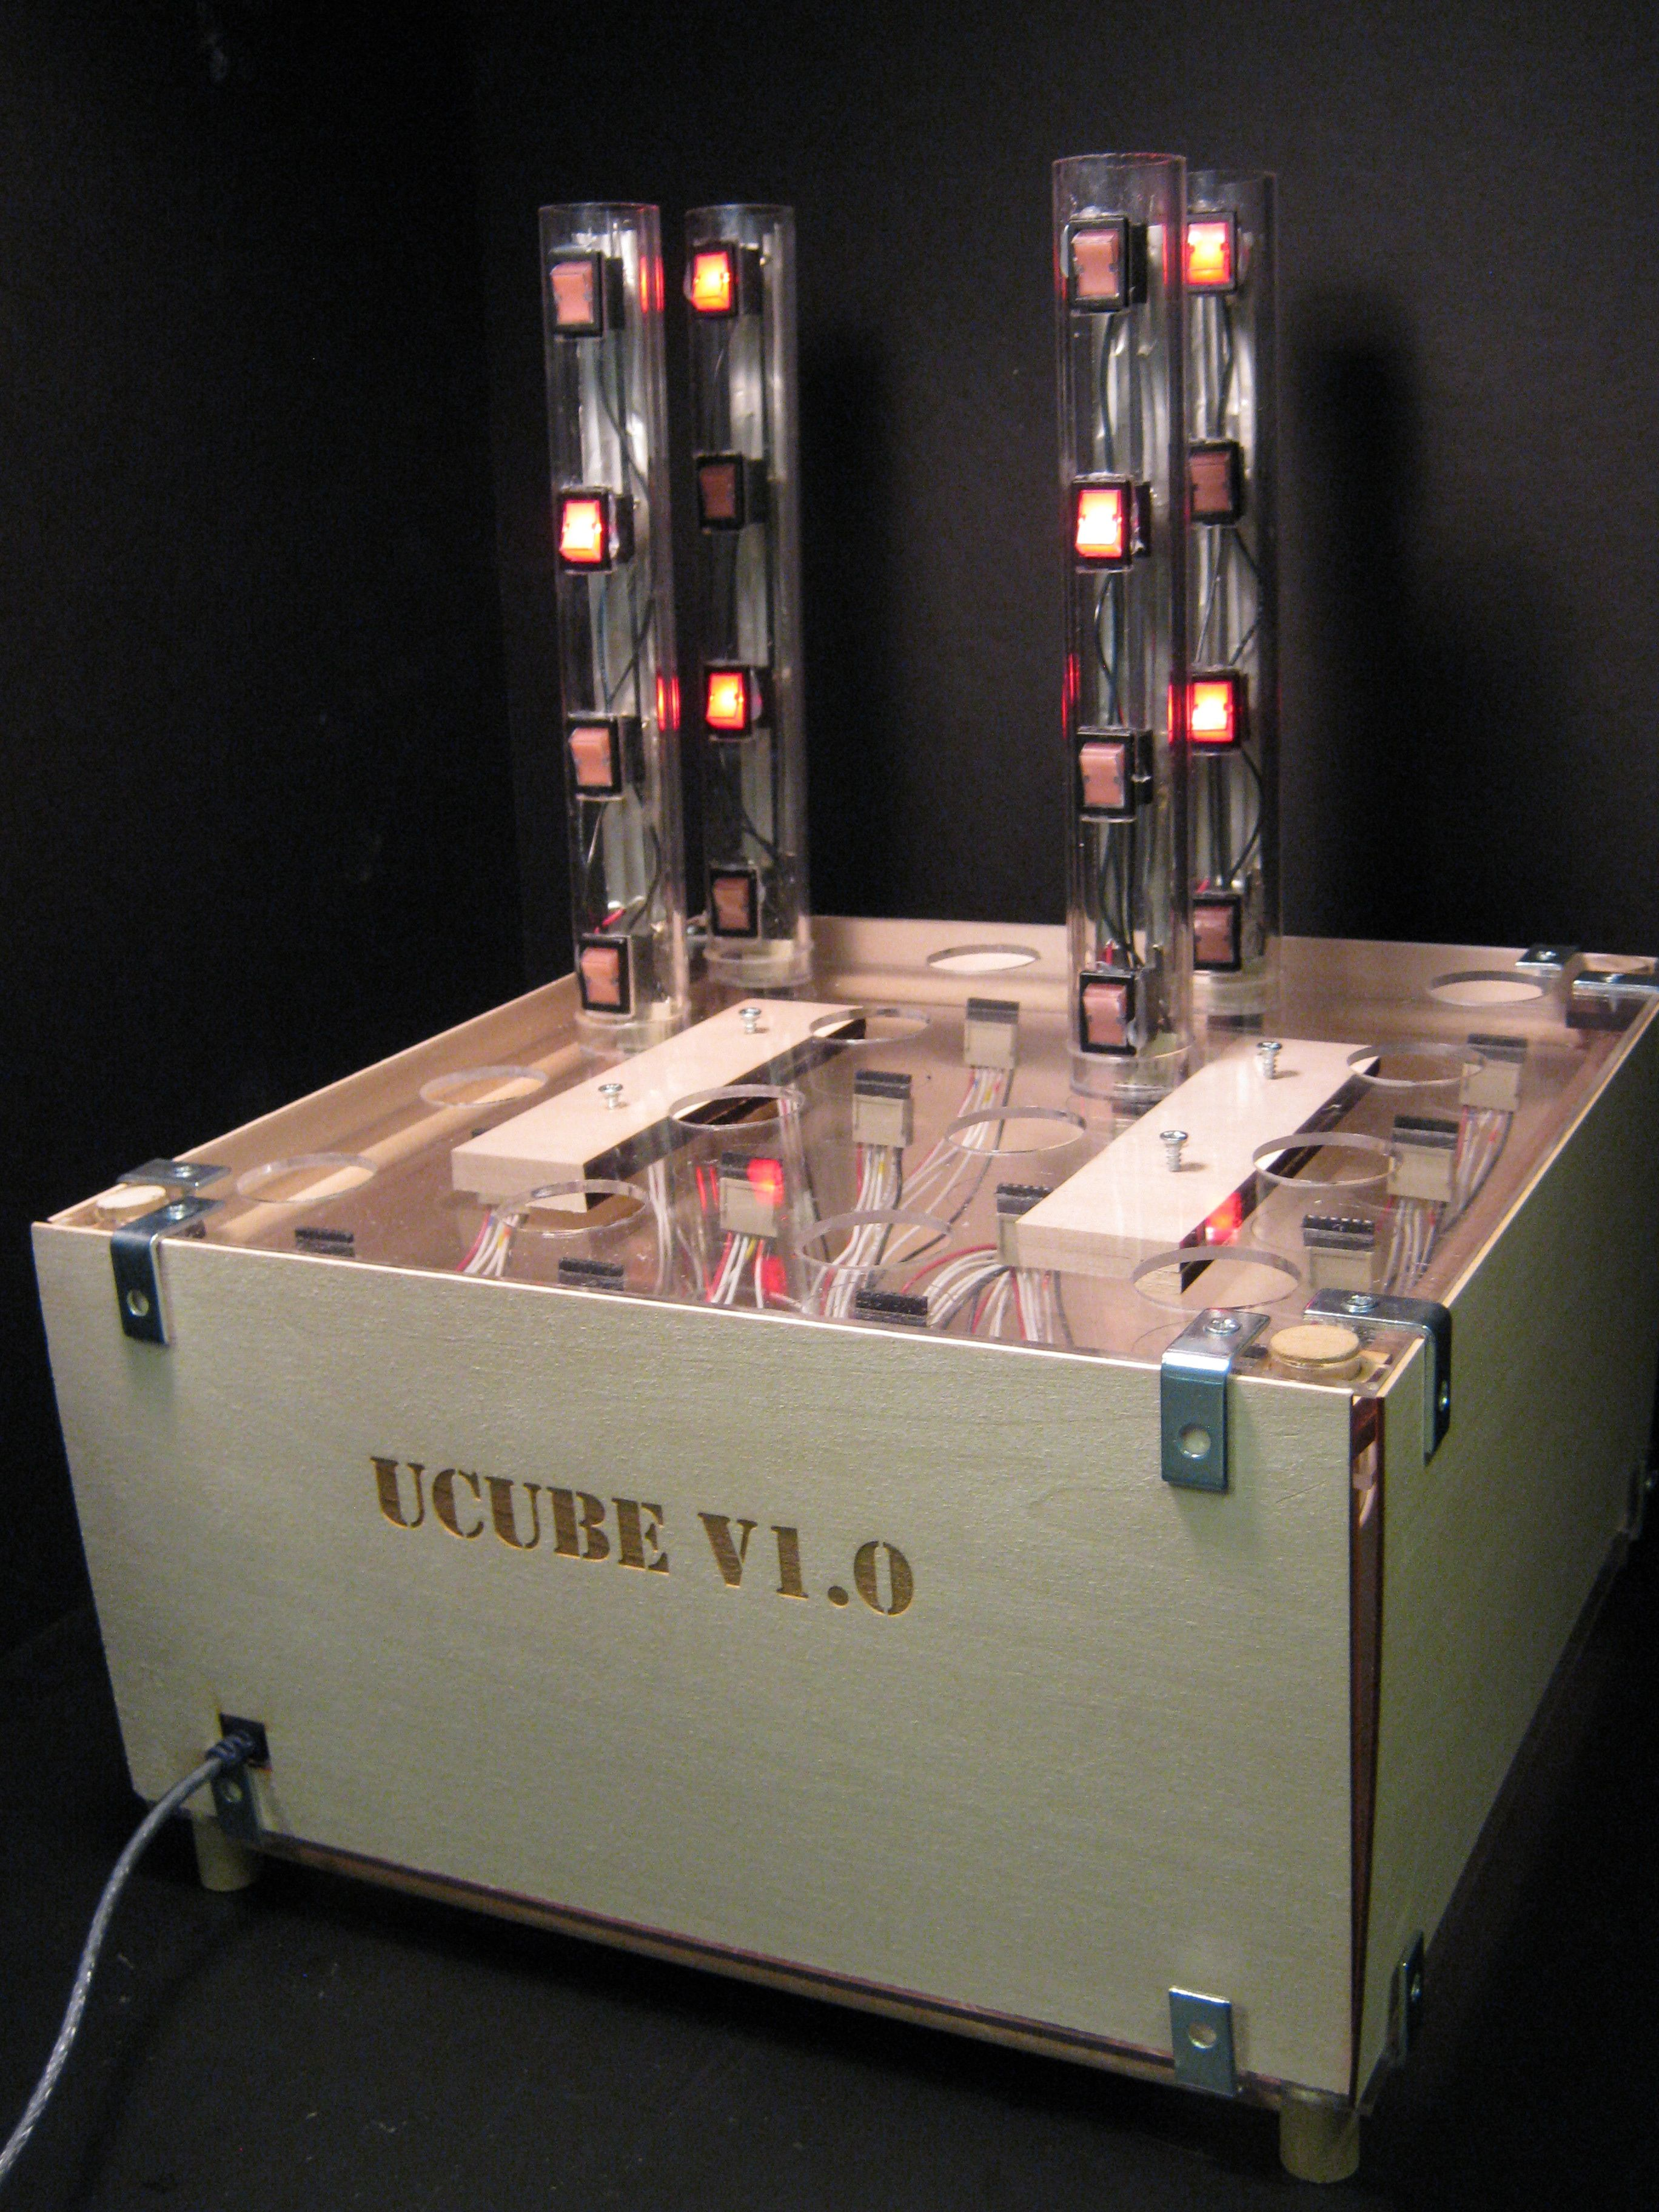
\includegraphics[width=.26\linewidth, height=2.3in]{images/ucube1_triPrism}&
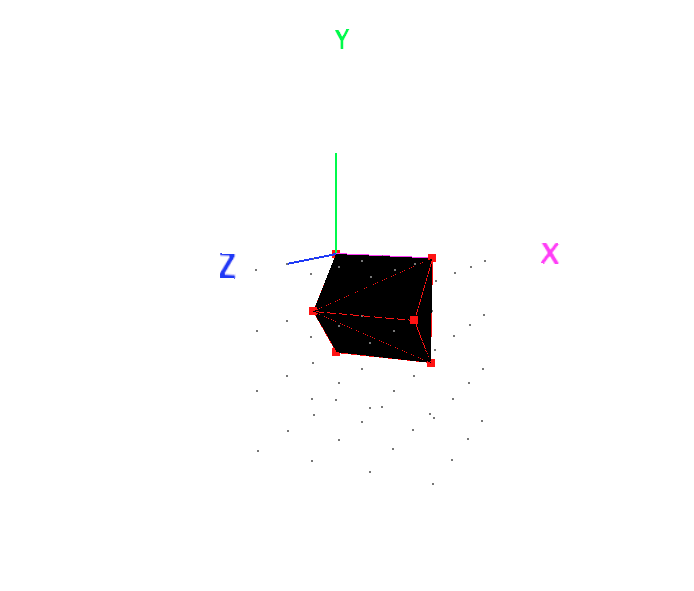
\includegraphics[width=.32\linewidth, height=2.3in]{images/ucube1_software} &
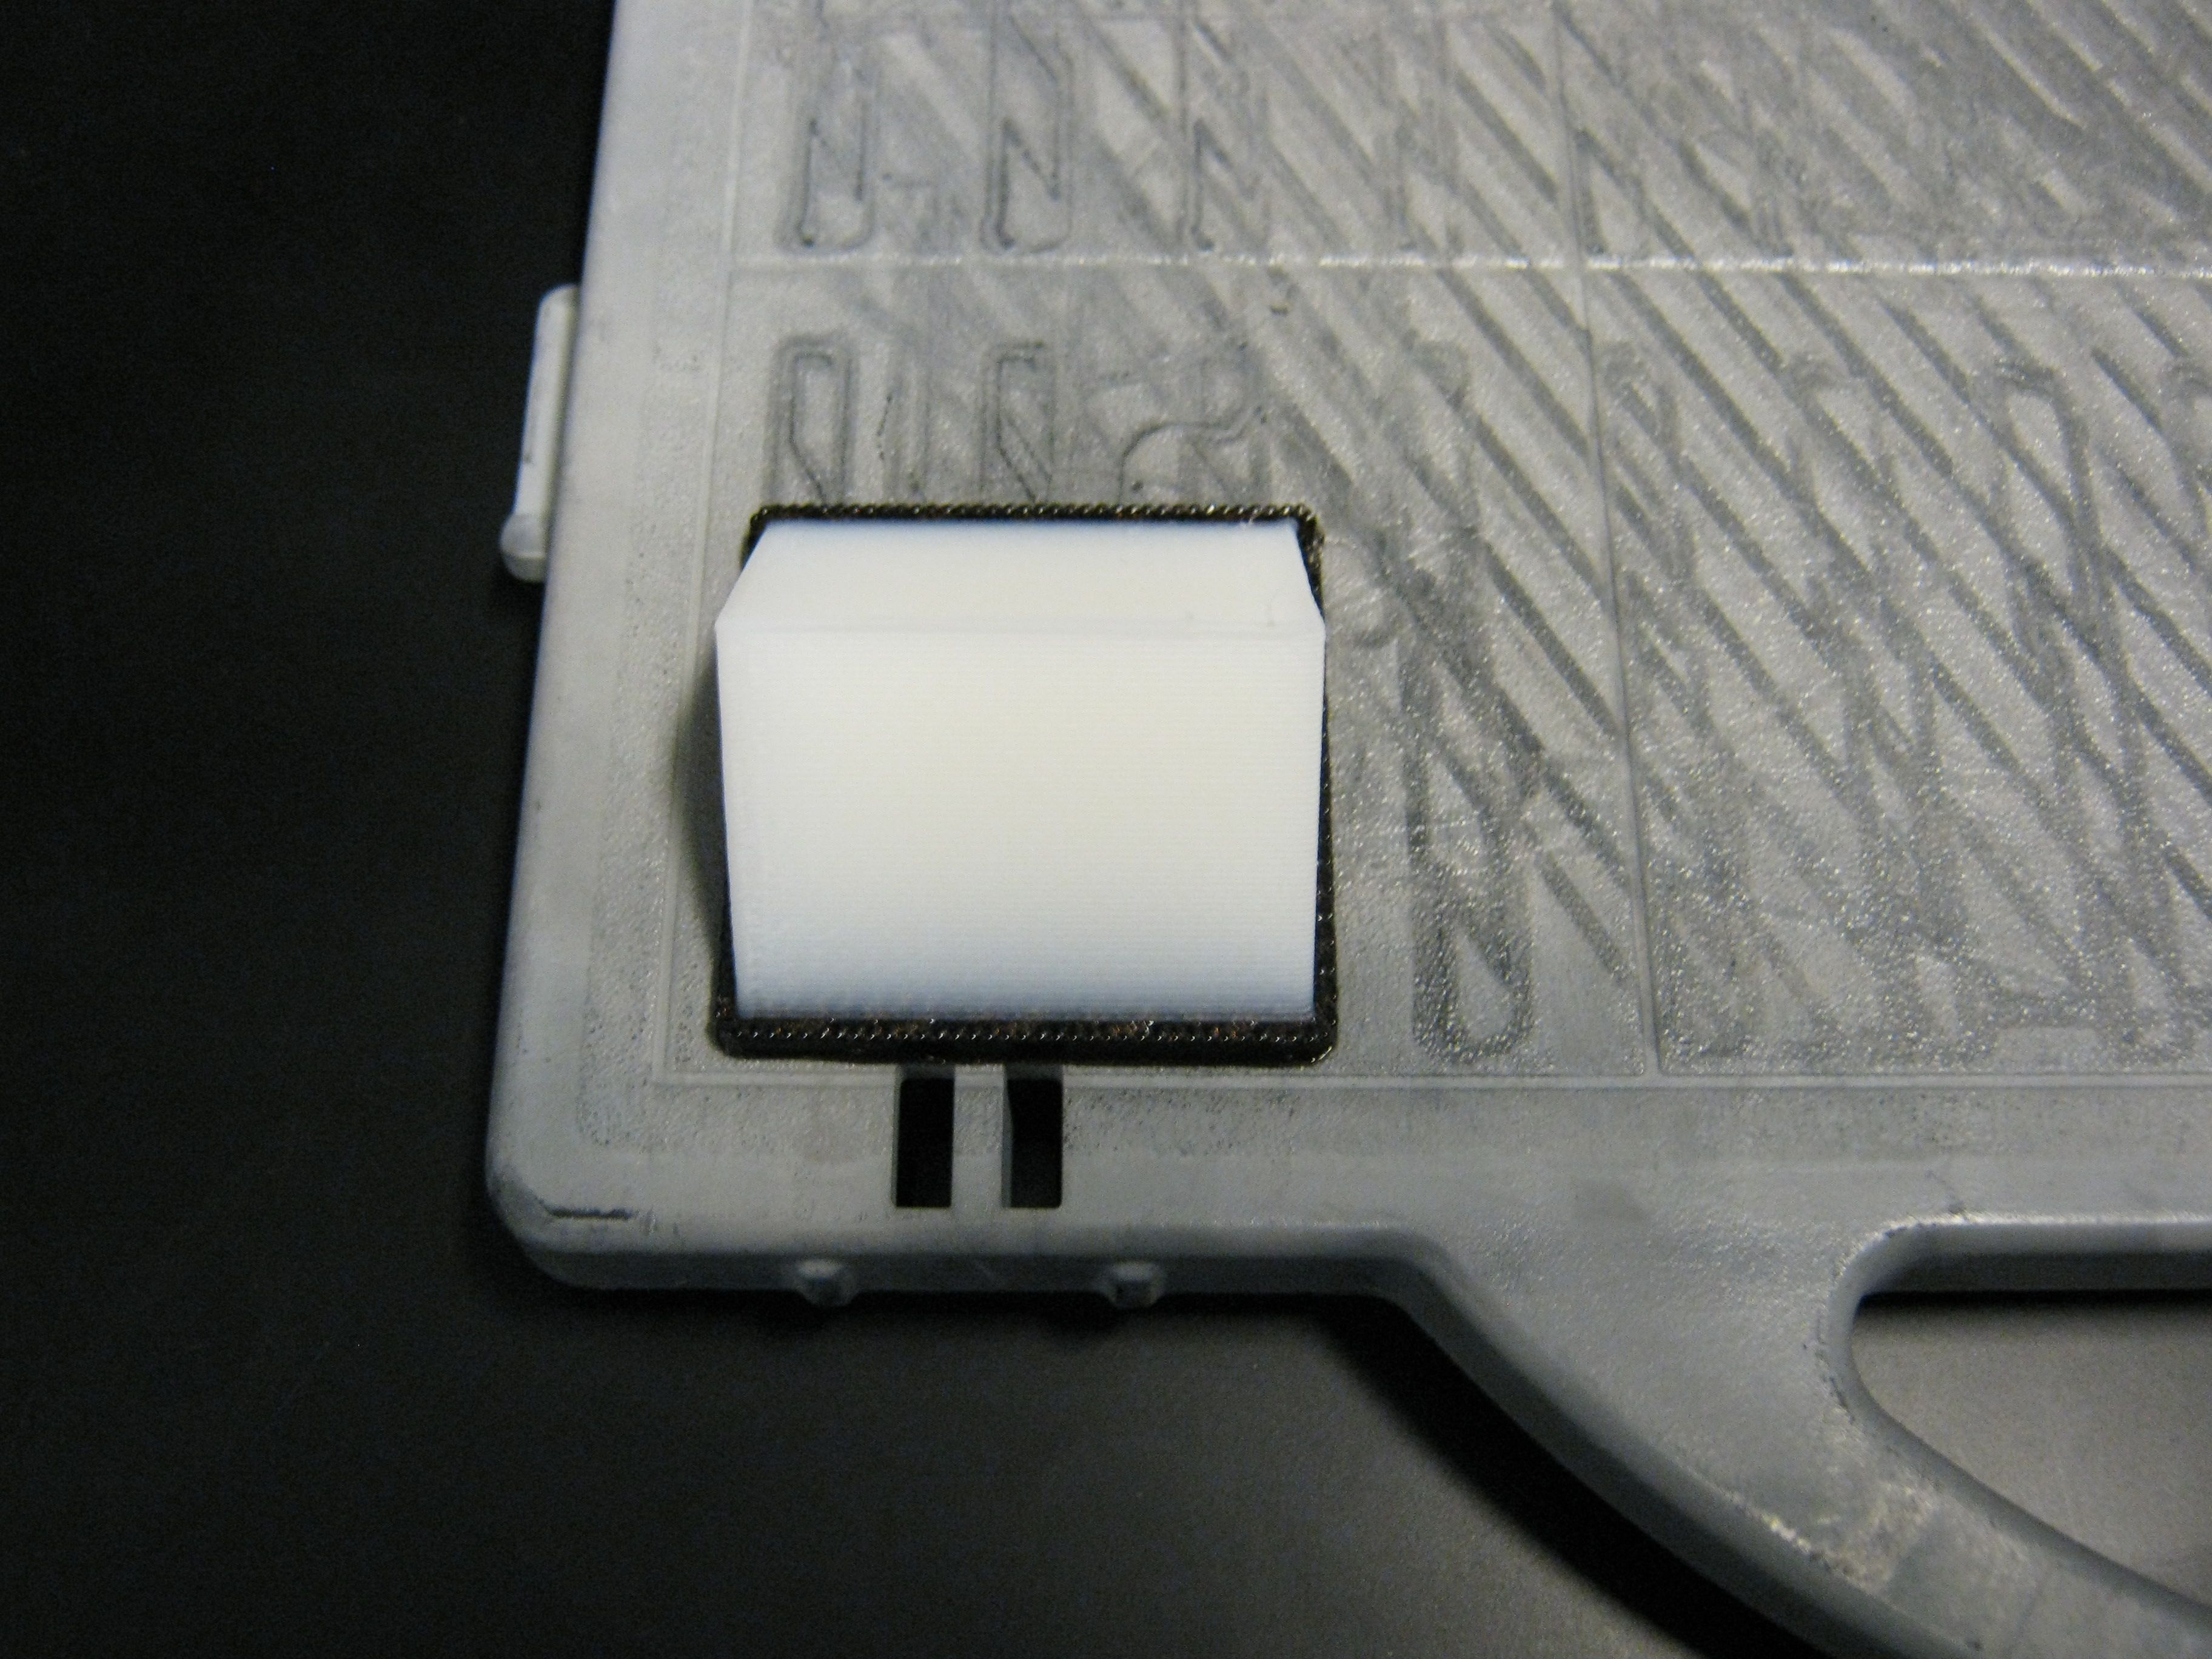
\includegraphics[width=.32\linewidth, height=2.3in]{images/IMG_0425}
\end{array}$
\end{center}
\caption{Left: The UCube device, with four towers and six lit switches,
representing the six vertices of a triangular prism. Center: An early version of
the UCube software, representing the convex hull formed with the six active
points from the picture to the left. Right: The resultant 3D print, exported
from the software to a 3D-printer friendly format.}
\label{fig:cubev1}
\end{figure}

\subsection{Limitations}

The astute reader will have picked up on some of the more obvious limitations of
the early system: as a three-dimensional modeling device, it is quite limited in
the scope of things it can effectively model, certain geometric shapes are
impossible to model on an integer lattice (a dodecahedron, for instance), a
4x4x4 resolution is clearly insufficient for complex shapes, and the inability
to create curved surfaces precludes most ``natural'' objects (such as human
faces) from being represented in a life-like manner. It is thus important to
differentiate this system (and the others mentioned in this chapter) from a
``professional'' 3D modeling system; our focus is on ease of use for novices, to
provide a visual and tactile bridge between 2D and 3D worlds, and to provide a
simple way to create shapes suitable for 3D printing. Even so, this does not
preclude us from attempting to make a more powerful, expressive, and stable
interface to present to users.



\section{SnapCAD}

Based on the feedback and observations from the two user studies we performed
with the UCube (discussed in chapter 4), a second, more powerful instantiation
of the UCube has been created. Called SnapCAD (formerly known as UCube v2) this
next generation device consists of a total input space of 7x7x7 points, forming
343 distinct coordinates (as opposed to the 64 points of the UCube). We focused
on two main design goals with the SnapCAD: greater expressive power and greater
stability in the system operation.

\subsection{Technical Implementation}
To start with system stability, then; custom printed circuit boards have
replaced loose wires, the towers are designed in Rhino\cite{Rhino} and 3D
printed to safely and securely house the towers, which are in fact printed
circuit boards of their own. Instead of a rickety housing, the top layer is
1/2'' acrylic which was milled on a CNC machine to precisely fit the newly
designed towers. The sides and bottom are hand-crafted wood, with channels cut
to allow the top and circuit board layers to easily slide in and out. The frame
is not glued on one side to allow for repair and maintenance. This side is
secured by custom metal brackets and screws. Each socket has its own printed
circuit board, held firmly in place by zip ties around a latticed acrylic layer
underneath the boards. The system has since traveled to the Denver Art Museum,
the Computer Clubhouse in Lakewood, Colorado, and ridden around in the back of
several cars without mishap (not to mention roughly 20 hours of user testing by
eager adolescents).

\begin{figure}[!ht] 
\begin{center}$
\begin{array}{cc}
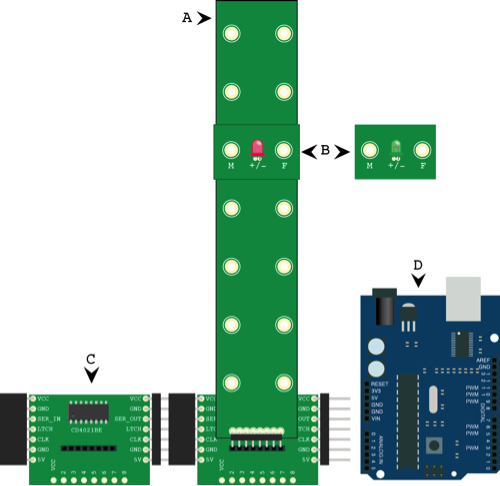
\includegraphics[width=.45\linewidth]{images/snap_schematic}
\end{array}$
\end{center}
\caption{A schematic of the SnapCAD technical design, showing a sample tower
(A), LED light element (B), shift register board (C) and Arduino (D). The Arduino
microcontroller's role is to send coordinates (and colors) of the LED lights,
once placed, to a desktop computer. A fuller description of this schematic is
provided in the accompanying text.}
\label{fig:snap0}
\end{figure}

The goal of expressiveness was met in two ways; by increasing the possible input
space from 64 points to 343, and by designing a system that allowed for each
point to be activated by more than one color of LED - effectively allowing for
multiple shapes to be modeled at once, or multiple ``players" to interact with
the board at once. Both of these solutions required changes in both hardware and
software from the UCube. Working on the scale of multiple hundreds of inputs
necessitated the design of custom circuit boards to relay information
effectively to the microcontroller. The Arduino Mega has only 54 digital
input/output pins, far too few to assign each line directly to an input, even if
one wanted to deal with tracking 343 i/o lines (which we most certainly did
not). Instead, we designed a circuit board around an input shift register chip
from Texas Instruments - the CD4021BE - that could effectively provide eight
more input lines per chip and operate with the Arduino's ATMega 328 Serial Peripheral
Interface (SPI) protocol, which requires only three lines from the Arduino. By
breaking out the pins on the CD4021BE so that they could be chained together (by
aligning the serial output of one chip to the serial input of the next chip,
while also passing along the latch and clock signals, the other two lines
necessary for the SPI to work)\footnote{We understand this section is somewhat
technical. A great introduction to using shift registers in this way can be
found at: http://www.arduino.cc/en/Tutorial/ShiftIn}. By arranging 49 of these
daisy-chained boards in a 7x7 grid, we had the framework to read in from 343
inputs in real time. Only one more problem had to be solved: at around 35
connected shift registers, we exceed what is called the ``fan-out'' of the
Arduino microcontroller - the number of connected input gates that a given pin
on the Arduino to drive a current load into. To get around this problem, the
clock and latch signals are put through a set of two ``buffers'' - in our case
CD4049BE inverting hex buffers - which can used for logic level conversion (the
inverting part, which we do not need, hence the second inverting buffer), but
also as a ``boost'' to drive the signal farther. One set of buffers was enough
to get our signals to the computer reliably.

This change in scale also meant rewriting most of the modeling software to
effectively handle the greater expressiveness of the physical system. The astute
reader may have noticed that while the CD4021BE adds eight inputs per board, our
system calls for a 7x7x7 array - so what were we to do with the extra input? The
dilemma actually ended up solving several problems; in the UCube firmware each
input triggered an (X,Y,Z) coordinate to be send out the serial port - by
switching to shift registers over SPI, we are limited to one character per input
- either a 1 or a 0. Normally, a serial string can be delimited in software by
looking for certain characters at the beginning or end of a communication, and
parsed accordingly, but we only had a string of 343 0's and 1's. Given that
most of the sockets would be returning a zero most of the time, by tying the 8th
input line high we could count characters and check for a ``1'' every eighth
character to ensure the serial string was correct - and since we were isolating
this character anyway, it was simple to throw it away afterwards and thus be
left with only the sets of seven digits describing the state of the inputs. The
problem of generating the proper coordinates from the input stream was then a
matter of creating a ``lookup table'' where the $nth$ character in the input
string array was the $nth$ element in an array of 3D coordinates.

\begin{figure}[!ht] \begin{center}$
\begin{array}{cc}
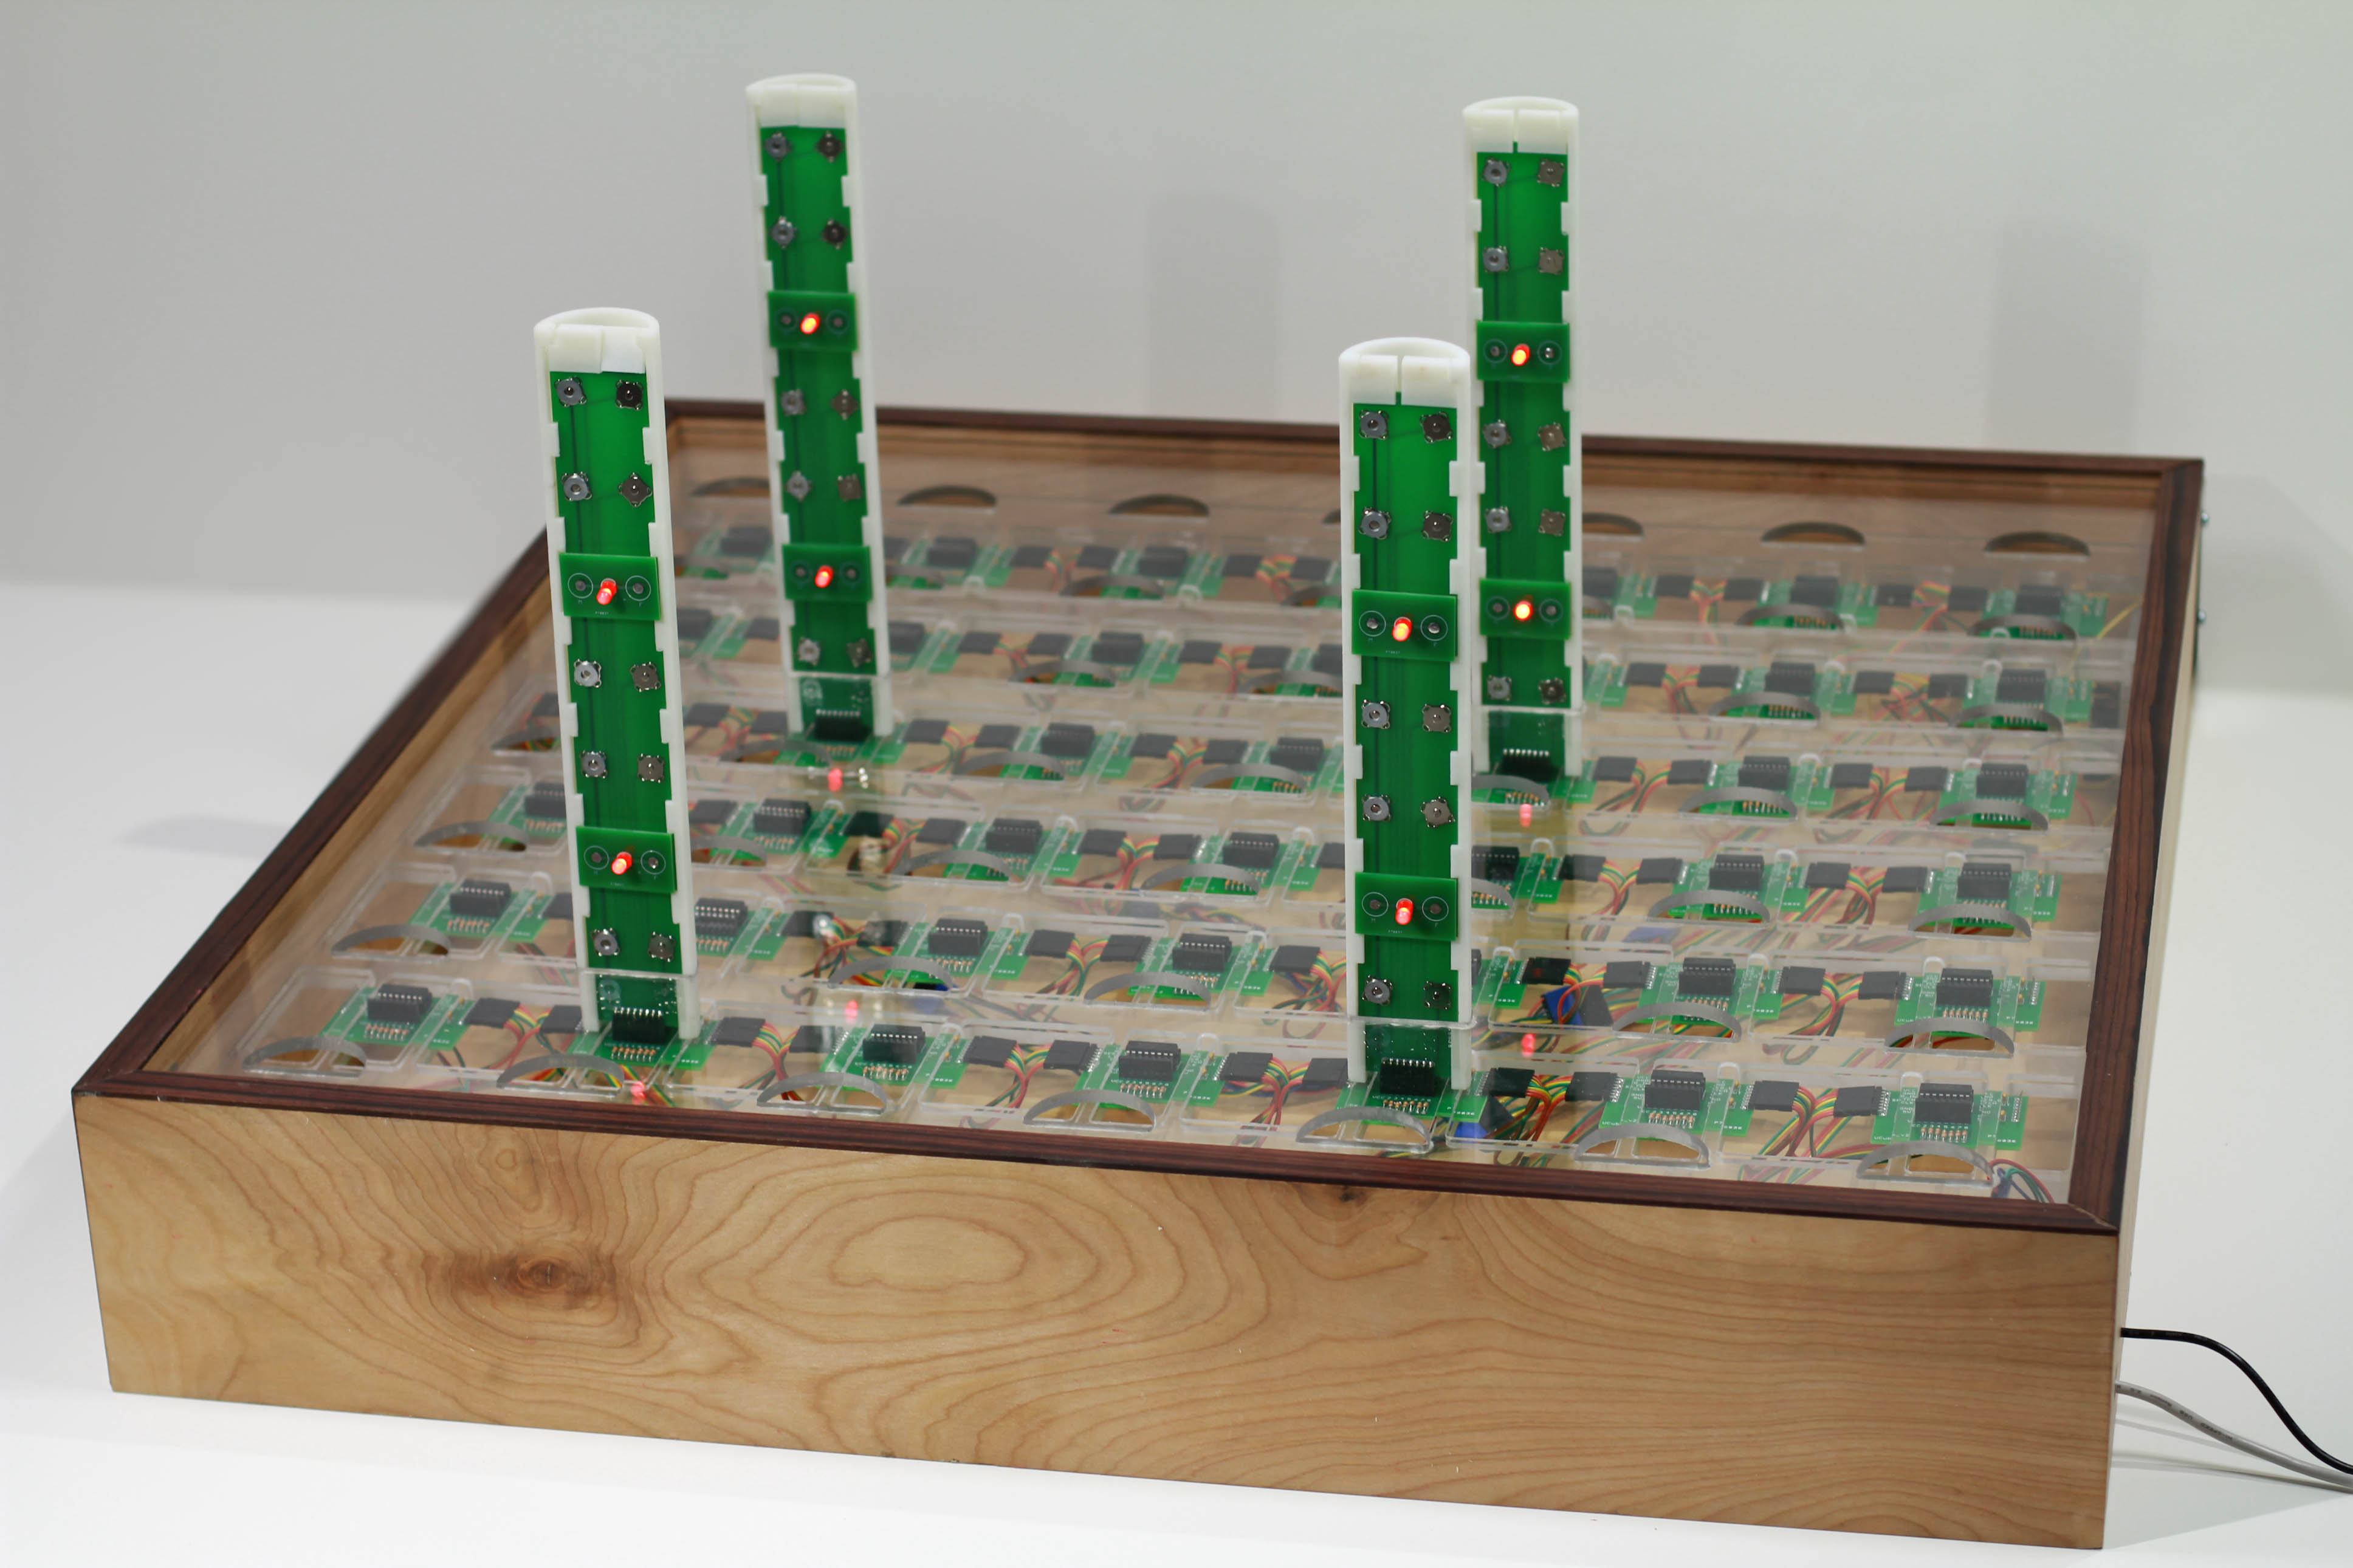
\includegraphics[width=.45\linewidth]{images/BeatriceFinal-9}& 
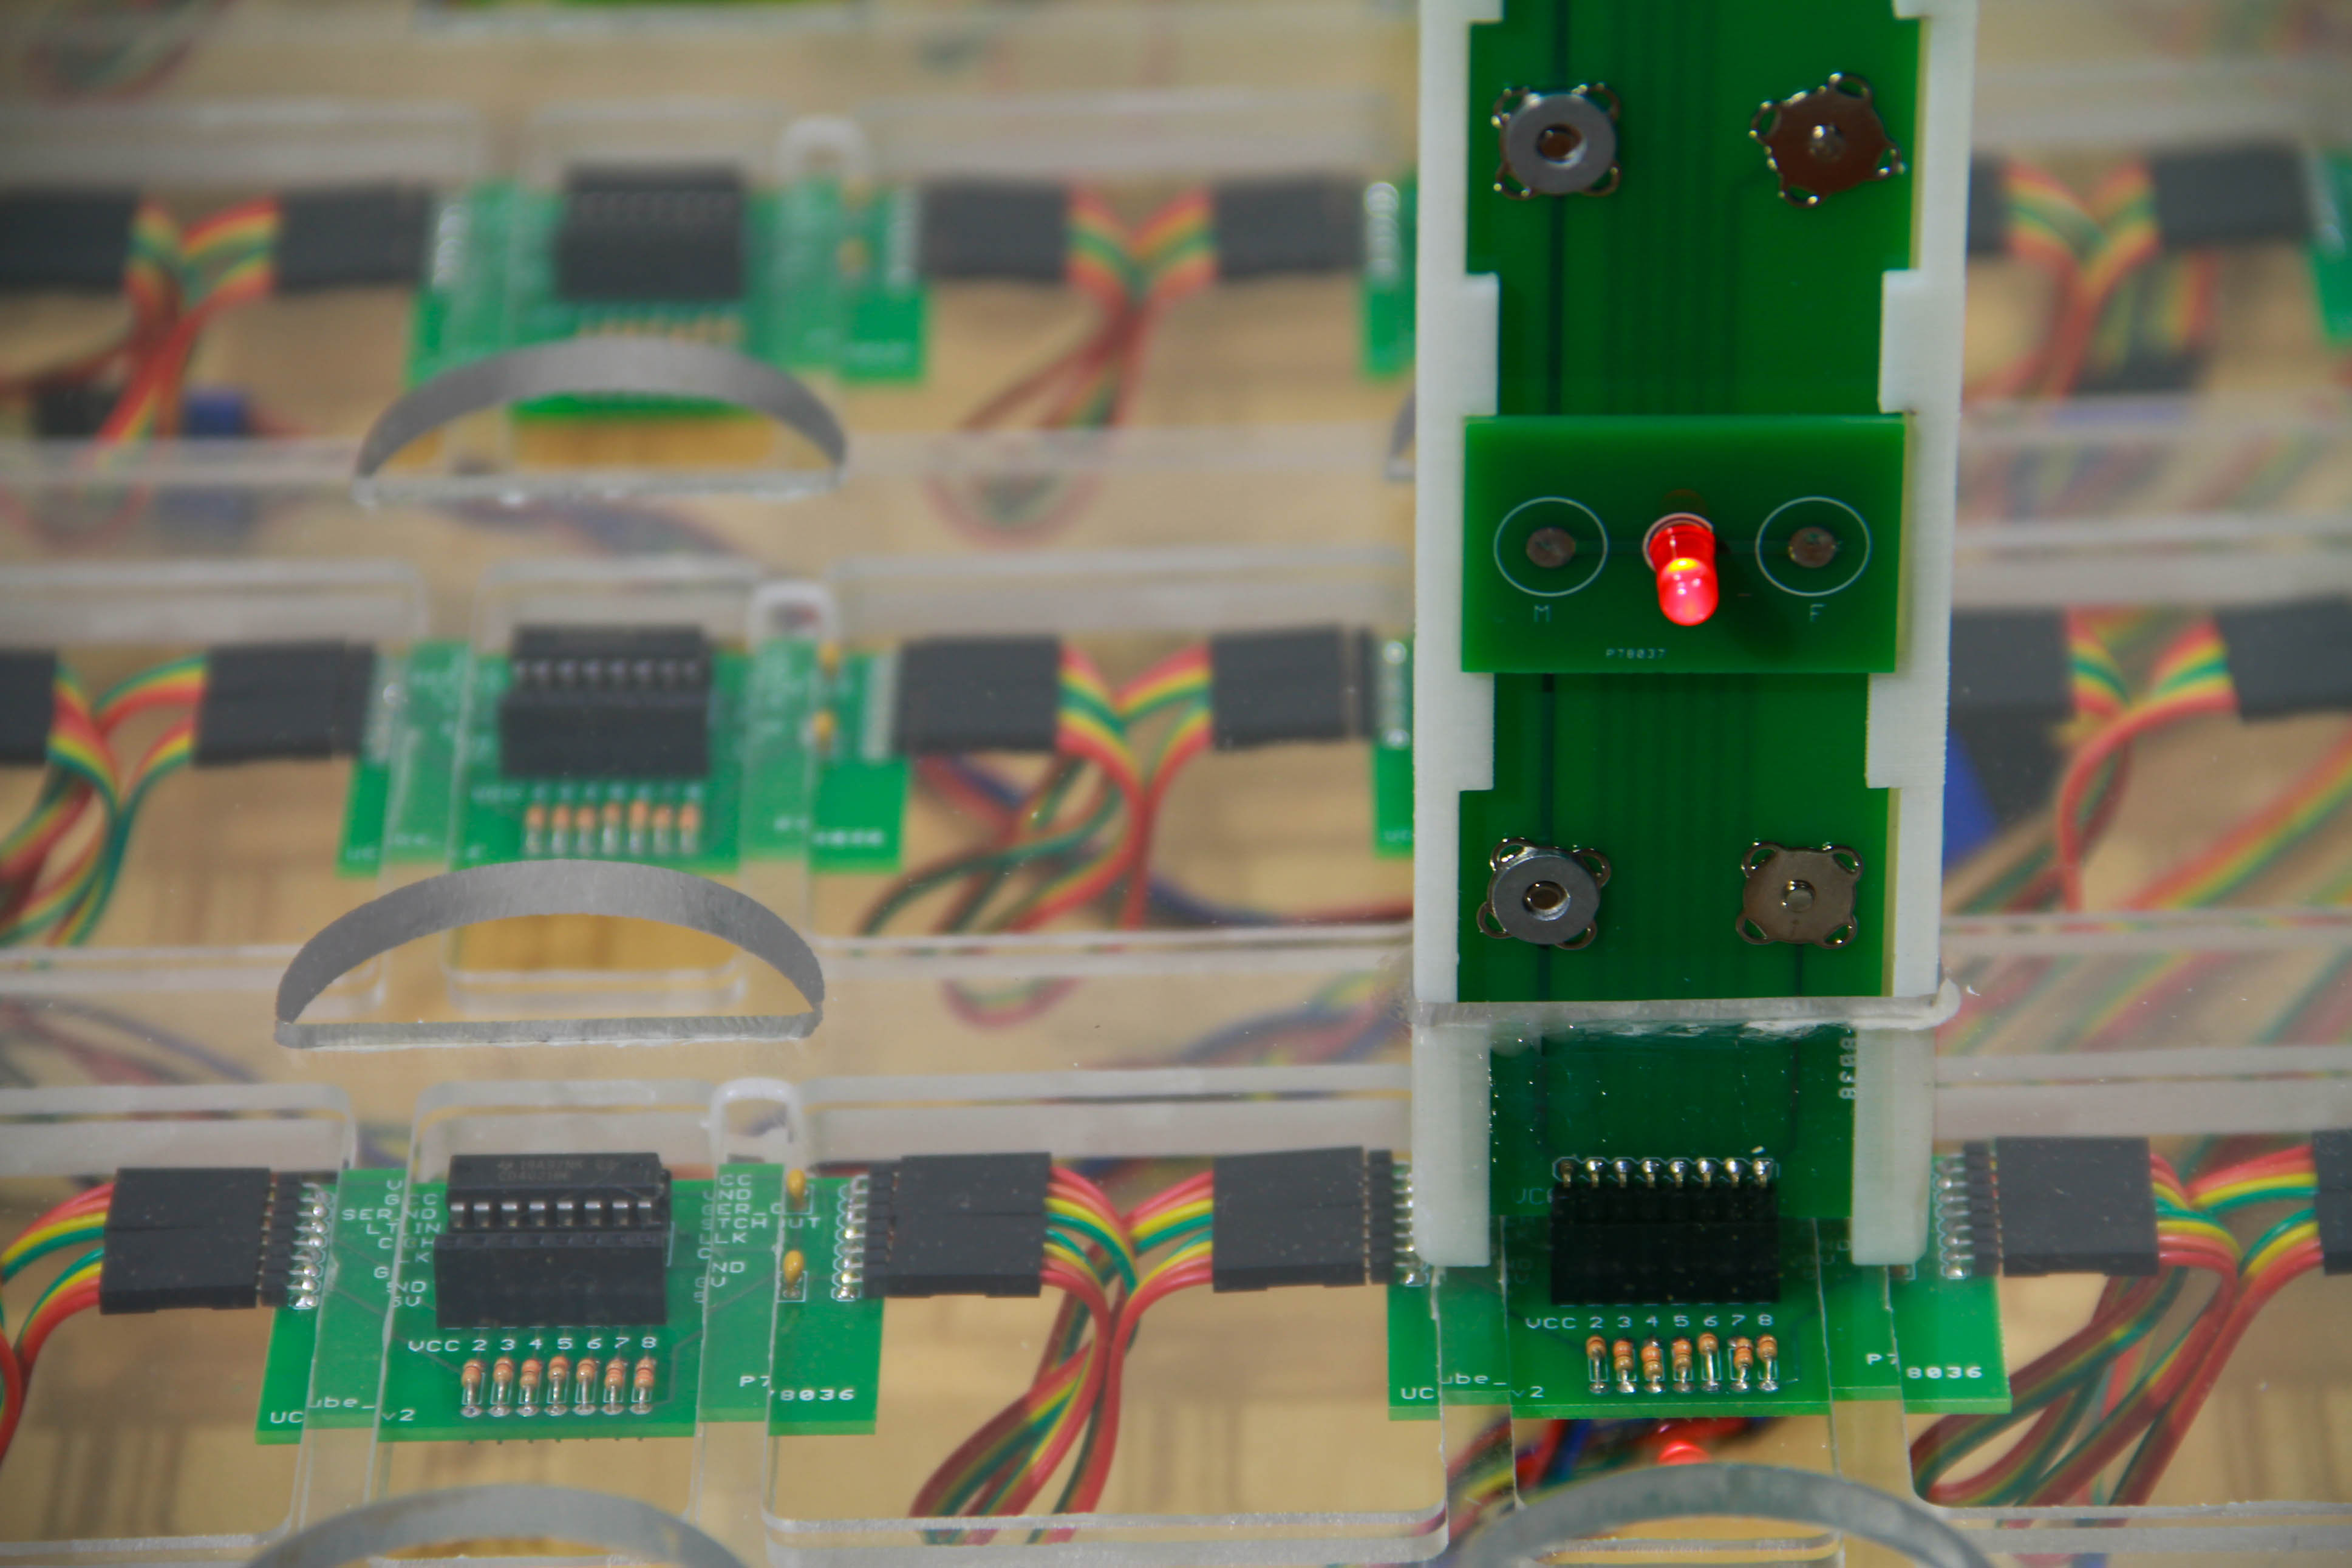
\includegraphics[width=.45\linewidth]{images/BeatriceFinal-14}
\end{array}$
\end{center}
\caption{
Left: the SnapCAD interface, showing four towers with two red LEDs each,
arranged in cube-like configuration. Right: a detail of the SnapCAD hardware -
the PCB tower is housed in a 3D-printed shell, which plugs into one of a chained
set of shift-register boards. The LED boards snap on to the towers via
conductive magnetic snaps.}
\label{fig:snap1}
\end{figure}

The other enhancement to the expressive power of the SnapCAD design is the
ability to use each socket in each tower with more than one color of LED. In
in order to make this a possibility, we had to find a way to make the LEDs
detachable from the tower and ``swap-able'' with other colors. This was achieved
by soldering conductive magnetic snaps directly into the circuit boards
themselves; the magnets act to both attach LEDs to the tower, but also to close
a circuit and light up the LED. We used snaps and not just simple magnets
because LEDs are polarized - they have only one correct orientation - and snaps
have a male and female part that could be used to indicate the correct
orientation. This multi-color capability can be seen in Figure \ref{fig:snap2}.

This ability to swap out different colors of LEDs not only results in the
ability to represent multiple shapes at once, but for the SnapCAD to become a
platform for all manner of multi-player interactions (e.g. games, puzzles, shape
matching contests), with each ``player'' assigned a unique color. To this end,
we have created a simple ``3D Tic-Tac-Toe'' implementation on the SnapCAD, and
imagined a sample scenario, explained in the next section. The SnapCAD version
of the software includes this ``multi-payer" ability as well as some additional
changes that include supporting multiple but separate convex hulls of different
colors, the ability to create and export shapes created from the minimal
spanning tree of a set of input points, and the ability to adjust the width of
the segments in the knot/path and minimal spanning tree modes.
The click-and-drag editing mode includes the knot/sequential path and minimal
spanning tree modes as well as the convex hull mode. We also adjusted the
knot-forming algorithm to handle paths that cross or self-intersect, as well as
providing a ``close knot'' button to complete a circuit in a shape, allowing for
even more kinds of 3D-printable objects.

% While significant work was been
% done to bring the UCube and SnapCAD to their current states, we believe not only
% that there is room for additional improvements to be made, but that, as opposed
% to focusing on a incremental but essentially similar interface as the subject of
% a thesis, it is far more intellectually interesting to focus on a class of
% objects that demonstrate multiple incarnations of a set of ideas.

\begin{figure}[!ht] \begin{center}$
\begin{array}{cc}
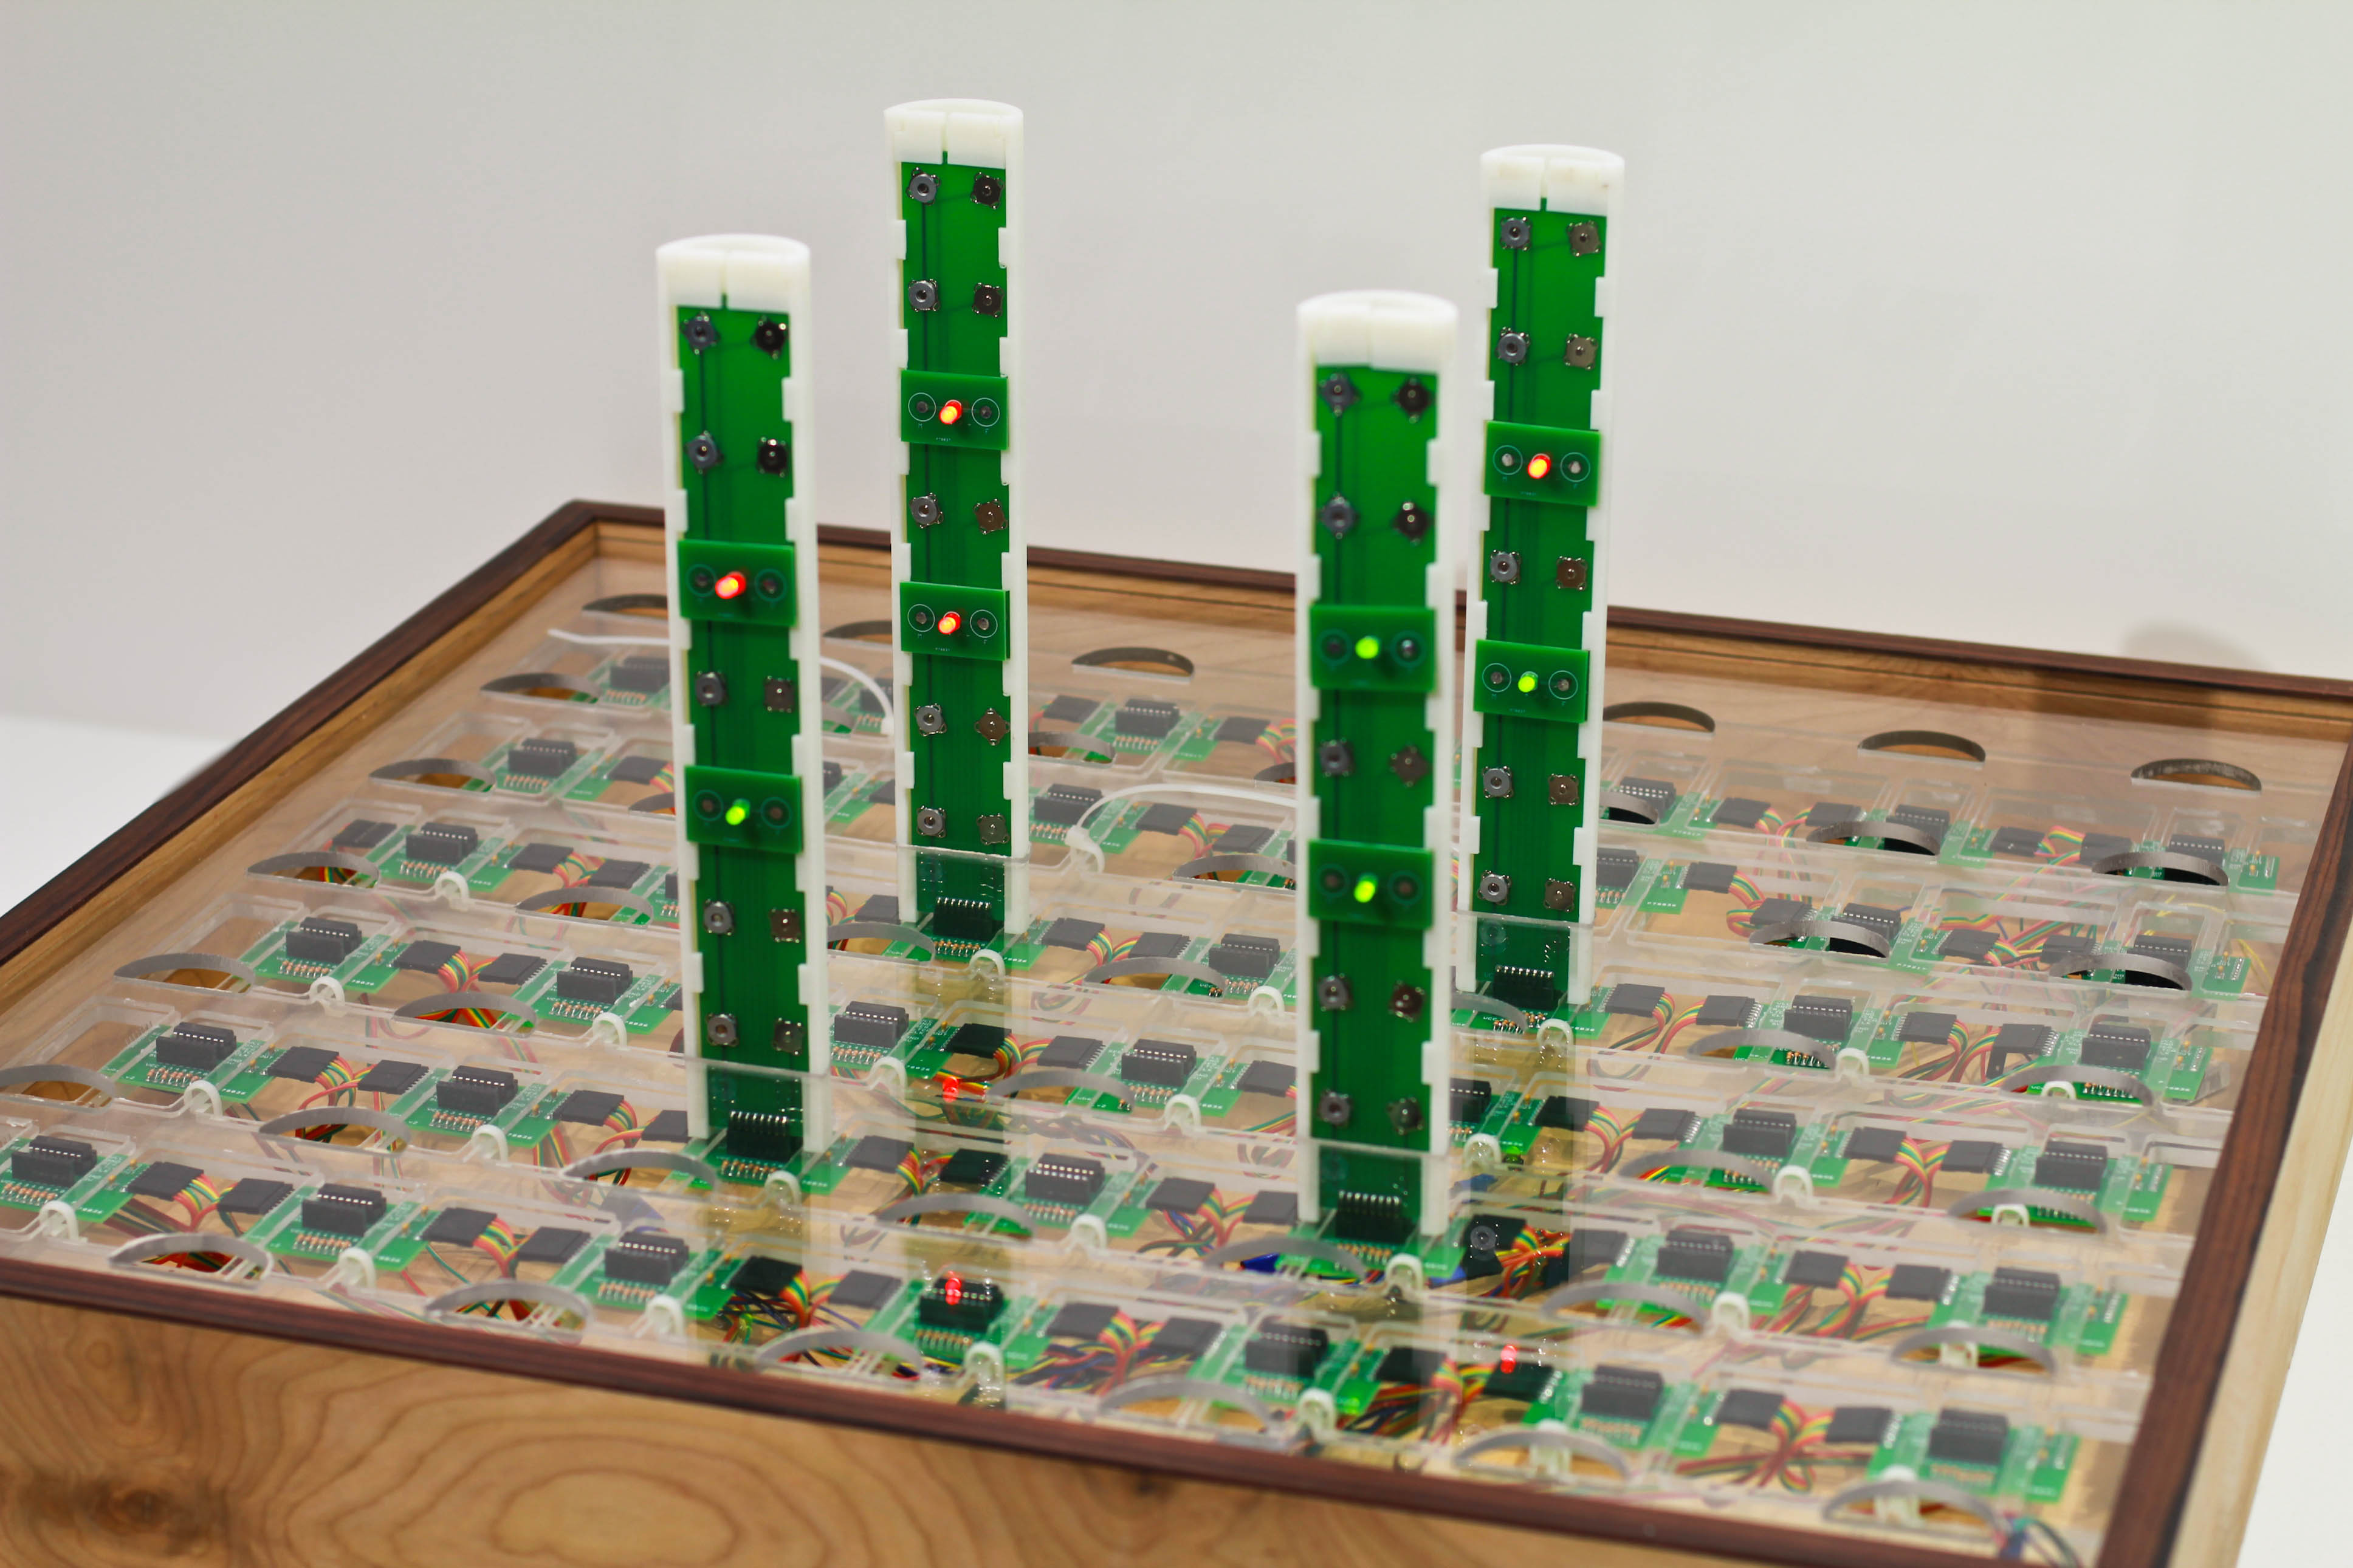
\includegraphics[width=.45\linewidth]{images/BeatriceFinal-2}&
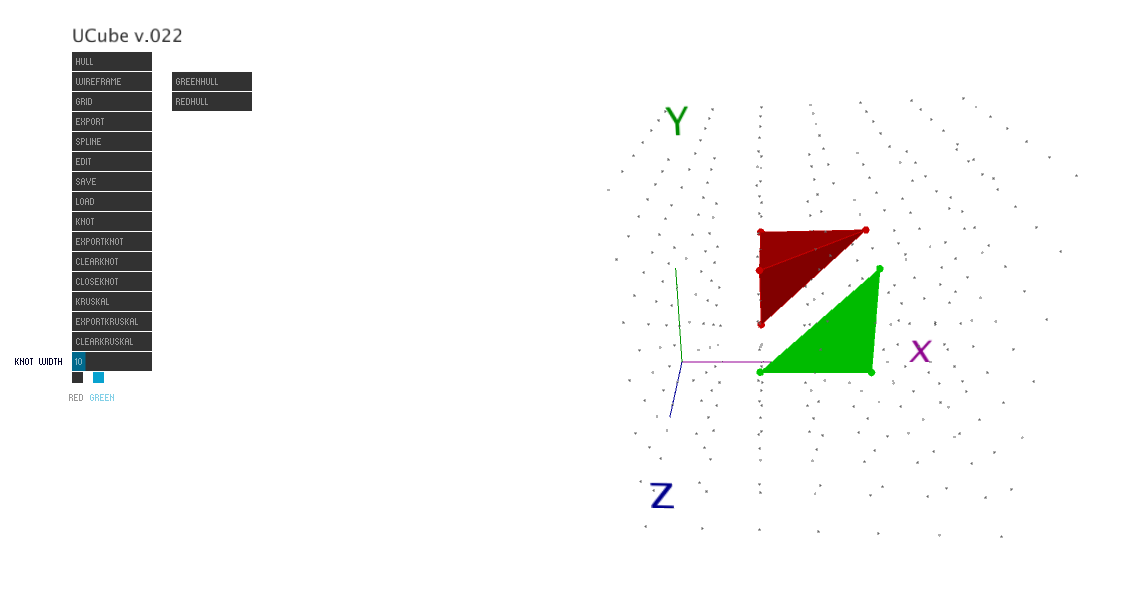
\includegraphics[width=.45\linewidth]{images/twoHulls} 
\end{array}$
\end{center}
\caption{Left: The SnapCAD software showing two convex hulls of different
colors. Right: the SnapCAD software showing a minimal spanning tree model.}
\label{fig:snap2}
\end{figure}


A note on the $7^3$ array in SnapCAD: in our user studies with UCube, we noticed
that users often encountered initial difficulties when required to ``find a
middle'' in the shape they were attempting to model, given an even number of
total grid spaces. For example, to model a pyramid on on a 4x4x4 grid, one needs
to construct a 3x3 subset of the 4x4 grid, using the middle point within the 3x3
set as the top of the pyramid. This influenced our decision to create an
odd-numbered layout, creating a more ``natural'' middle point in the hardware.




\subsection{A Sample (Red/Green Player) Strategy Game for SnapCAD}

In this use case, we make use of the two-color capability of the SnapCAD to
suggest a hypothetical game, or genre of game, that could be created with the
system. The imagined game in question is a geometric strategy game between two
players, ``Red'' and ``Green''. At the outset of the game, each player is given
four lights of her own color; the two of them are told to place their lights at
the eight corners of a cube in the positions shown in the photograph shown in
Figure \ref{fig:snap3} on the upper right.

\begin{figure}[!ht] \begin{center}$
\begin{array}{cc}
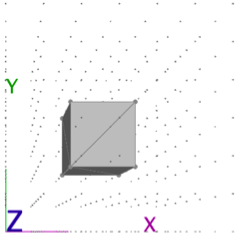
\includegraphics[width=.4\linewidth, height=2.2in]{images/snap_game1}&
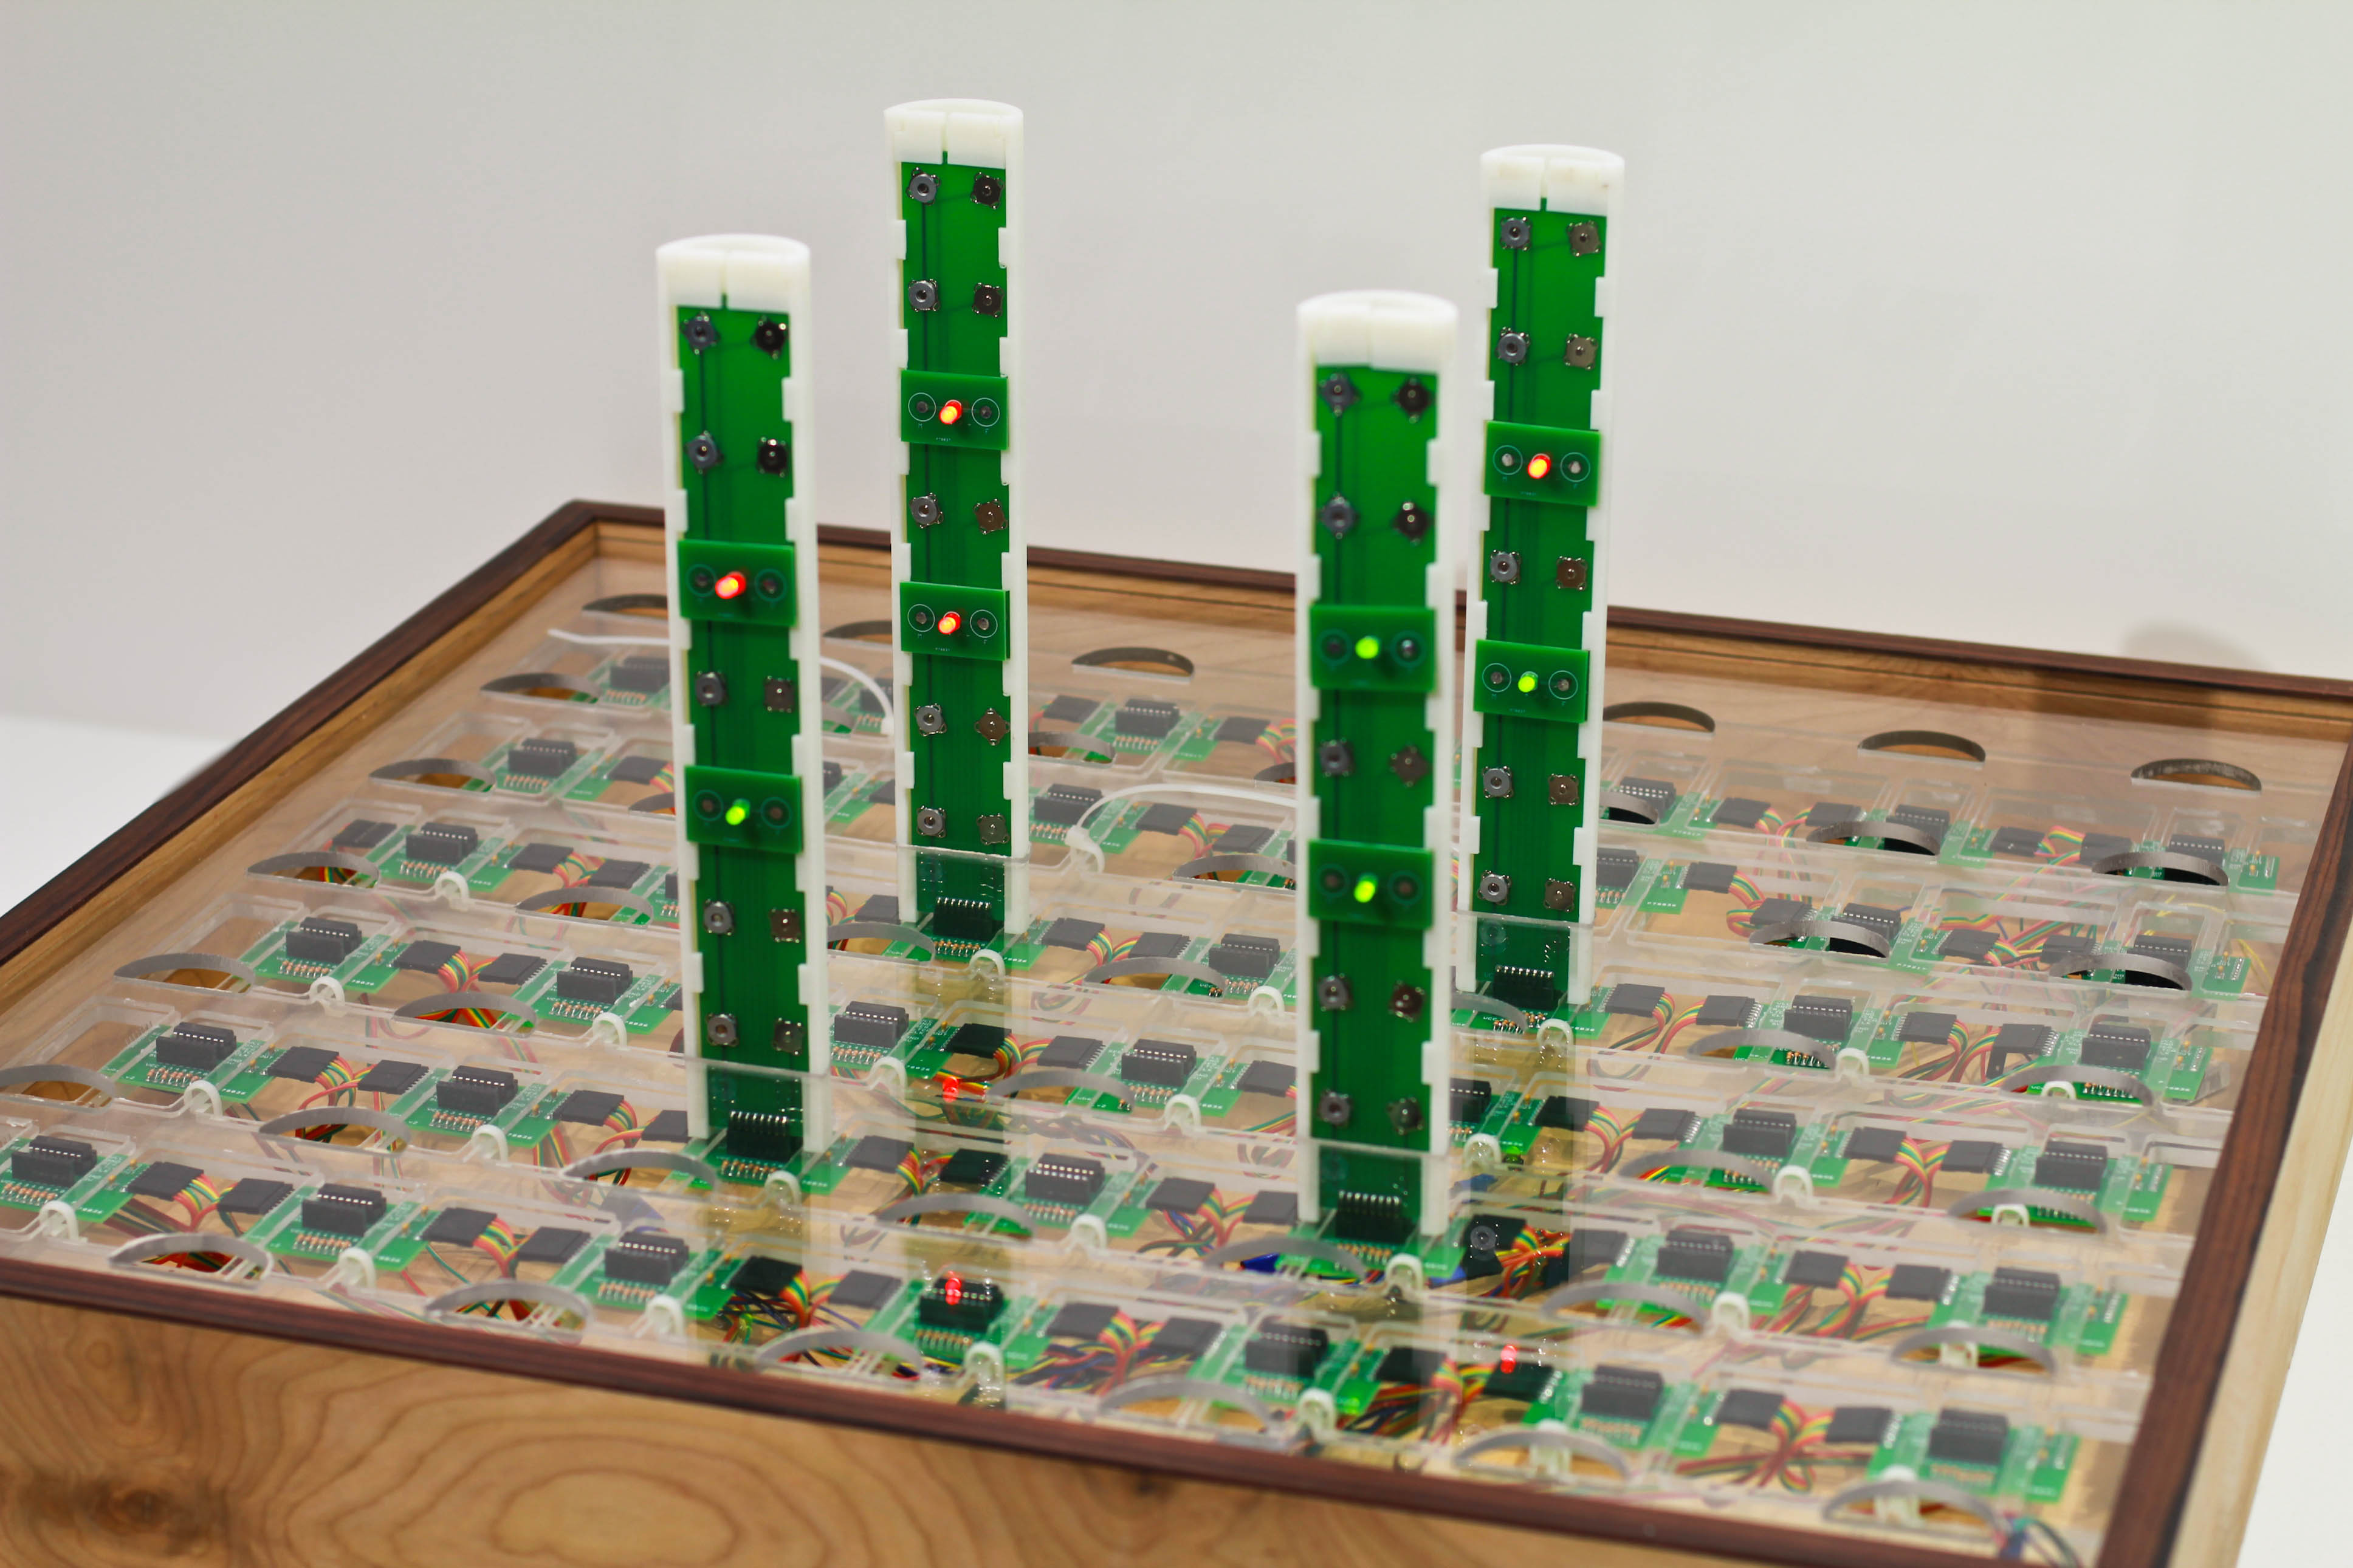
\includegraphics[width=.5\linewidth]{images/BeatriceFinal-2} \\
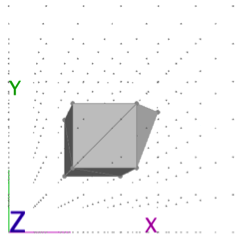
\includegraphics[width=.4\linewidth, height=2.2in]{images/snap_game2}&
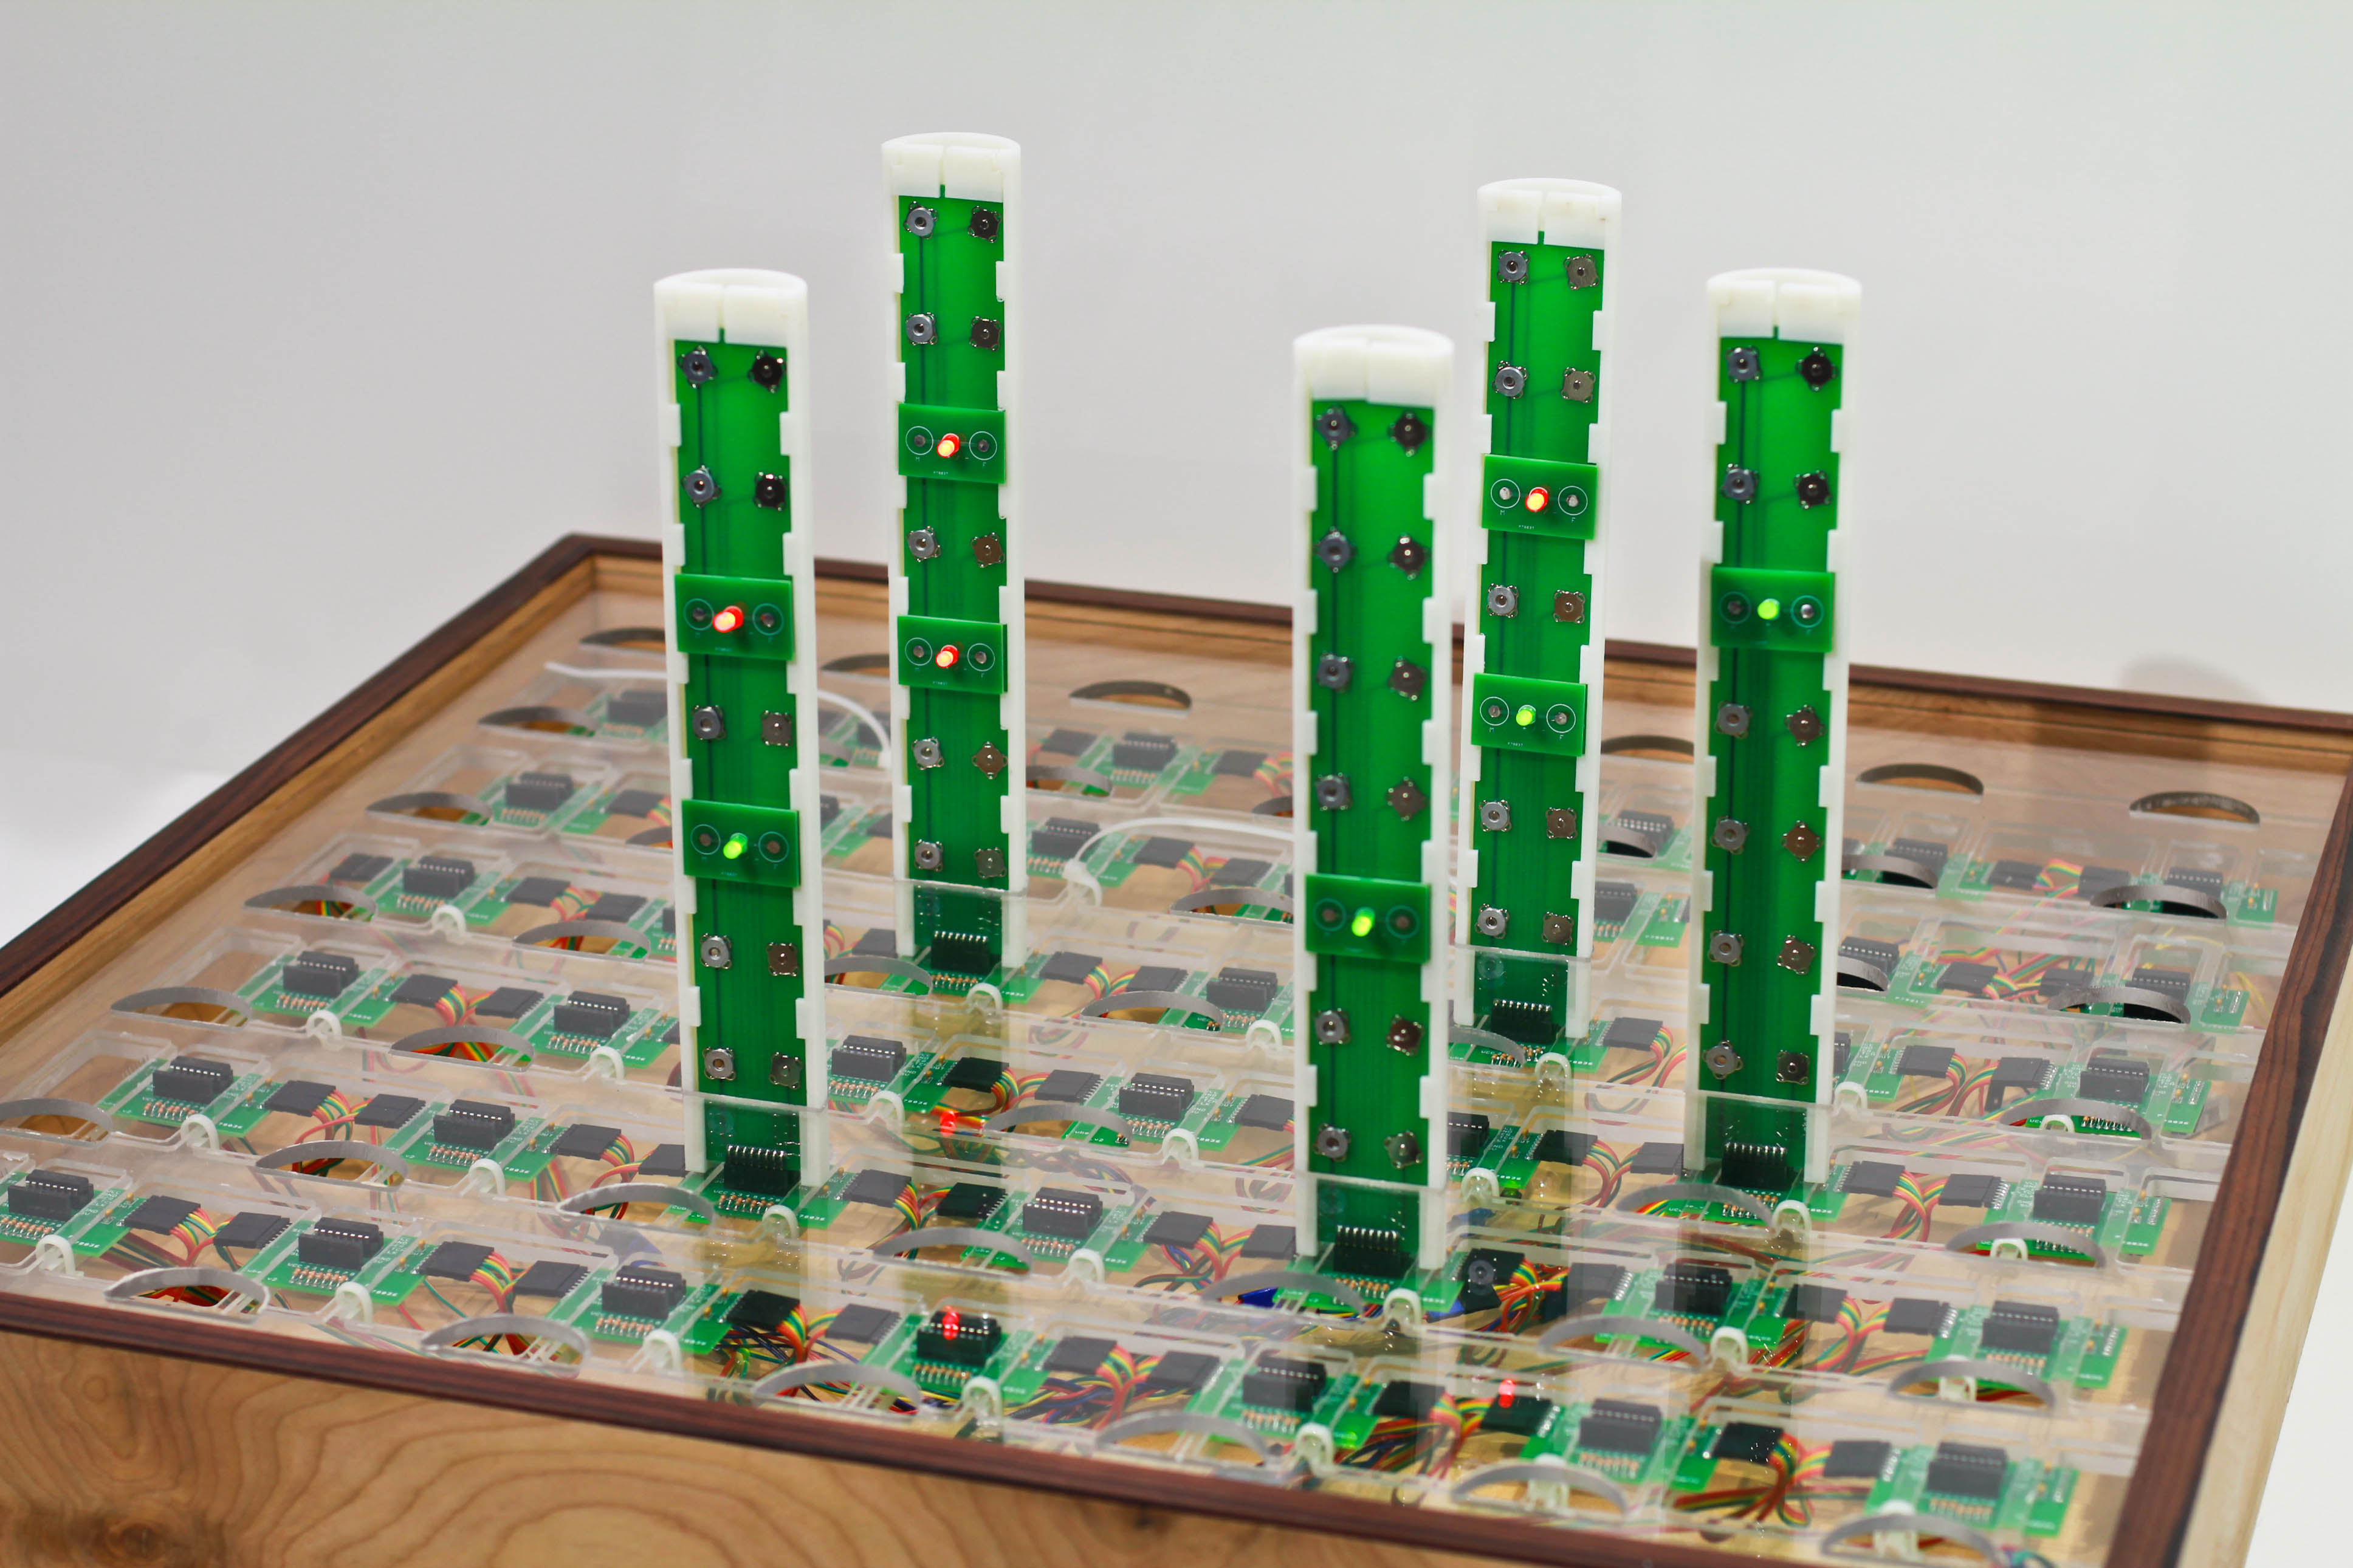
\includegraphics[width=.5\linewidth]{images/BeatriceFinal-3}
\end{array}$
\end{center}
\caption{Left: The SnapCAD software showing two convex hulls of different
colors. Right: the SnapCAD software showing a minimal spanning tree model.}
\label{fig:snap3}
\end{figure}

Now, the computer could display the convex hull of the present set of lights (a
cube), as shown in Figure \ref{fig:snap3} on the upper left; and then (in our
scenario) the computer tells the Green player to move one of her lights to
create the new convex hull shown at the bottom-left of Figure \ref{fig:snap3}.
Thus, the Green player's job is to change the ``cube'' hull to the new hull with
one move of one green light. A correct answer to this challenge is shown in the
photograph of Figure \ref{fig:snap3} at the bottom-right; and if the Green
player makes this correct move, the Red player is now given the (current) convex hull
and yet another hull that could be created with one move of a red light. In this
fashion, the two players take turns moving lights of their own color to produce
a new overall configuration of lights at every step, until one player fails to
solve the current challenge, at which point the game is over.
There are, of course, many variants or extensions of this game that could be
imagined (for instance, a player might be asked to shift two lights, or to add a
new additional light in her color, to create a new convex hull). The purpose of
this example is simply to show that, with the inclusion of two available colors
for spatial points with SnapCAD, a sizable potential landscape of geometric
activities and puzzles becomes feasible.



% \section{Proposed Work: Technical Additions}
% The proposed work is in two sections: technical additions and
% evaluation. This section deals with the technical additions to the proposed
% devices: SnapCAD and PopCAD.
% 
% \subsection{SnapCAD}
% 
% With 343 potential points, a click-and-drag editing tool, and three separate
% modeling modes (convex hull, knot/path, and minimal spanning tree) the SnapCAD
% is capable of generating countless 3-dimensional forms.
% Although the potential for additional modeling tools is certainly a possibility
% (we have yet to experiment with curved surfaces, for instance) we believe that
% the multi-player `platform' aspects of the SnapCAD system are the most ripe for
% development. We already have two colors of LED boards, the ability to display
% two colors of convex hulls, and a 3D implementation of a two-player tic-tac-toe
% game. Displaying multiple colors of the path/knot and minimal spanning tree
% modes should be fairly straightforward to implement.
% We would also like to expand and change the colors currently being used - we
% currently use red and green LEDs, which would be problematic for anyone with
% red/green color blindness. We propose using three colors: red, blue, and purple.
% This not only allows for up to three-player interactions, but could help to
% solve a deeper problem: representing in hardware a node occupied by two players.
% Using an idiom where solely-occupied nodes are either blue or red, and a jointly
% occupied node is purple, we can then expand the types of games, puzzles, or
% modeling activities the SnapCAD system can support. Once these improvements are
% made we can expand the activities supported on SnapCAD. Developments include
% two-to-three player games like tic-tac-toe as well as games built
% off of the modeling capabilities of the SnapCAD (e.g. match the model generated
% by the computer, model a sequential path through a generated maze, place points
% on or interior to the convex hull until there are no more to be found). Colors
% can also be used for certain as-yet unexplored modeling operations (e.g., the
% set union, intersection, or difference). While some of these operations may
% prove difficult or even impossible, these are all avenues worth exploring, as
% they all point towards the extensibility and potential expressiveness of SnapCAD
% as a platform for future development.

\section{PopCAD}

Our motivations for creating a third, alternative interface to the UCube and
SnapCAD stem from the desire to explore this intellectual space more generally;
it is far more interesting to discuss a \emph{class} of tangible interfaces for
scaffolding digital fabrication than it is to discuss a singular device. To this
end, we looked at some of the weaknesses of SnapCAD and towards technologies we
had yet to explore. While SnapCAD can admirably perform a number of modeling
tasks, it was always envisioned as one device amongst an ``ecosystem'' of next
generation fabrication tools. It has strengths, but obvious weaknesses as well;
in particular, the SnapCAD hardware was expensive to produce, and so would be a
difficult proposition for some schools or fab labs to produce or purchase; it is
also rather unwieldy and unportable - it is moderately heavy, fairly large (over
30 inches square), and has many separate pieces (like the towers and LED boards)
that could break or go missing. Thus, an interface with cheaper and more
portable materials was desirable.

To address these issues we chose to build a pop-up book combining traditional
paper-crafts and paper-friendly electronic components such as copper or
conductive tape and conductive inks.
In recent years, revolutionary work has been done in combining electronics and
paper
crafting\cite{Qi:2010:EPE:1709886.1709909}\cite{Mellis:2013:MMC:2460625.2460638},
leading to new techniques and new uses for traditional materials. Paper is
inexpensive (especially when compared to circuit boards), light, and easily
portable, making it an ideal material choice for a device that would not suffer
the same limitations present in the SnapCAD. Although we often think of
``paper'' as a rather static material, there are in fact many variations in the
size, weight, color, transparency, and composition of contemporary paper
products. We will cover the two paper-based prototypes we created in this vein,
dubbed ``PopCAD v1'' and ``PopCAD v2''.

\subsection{PopCAD v1}

For the initial prototype, we use a simple construction paper as it provides a
balance between strength and flexibility as well as having a consistency
well-suited to laser etching and cutting. The pop-up book (named PopCAD) has a
3x3x3 array of 27 points which are evenly spaced three inches apart on a 12'' x
18'' paper surface. The book folds on a single center crease making the closed
footprint of the book roughly 12'' x 9''.

\begin{figure}[!ht] \begin{center}$
\begin{array}{cc}
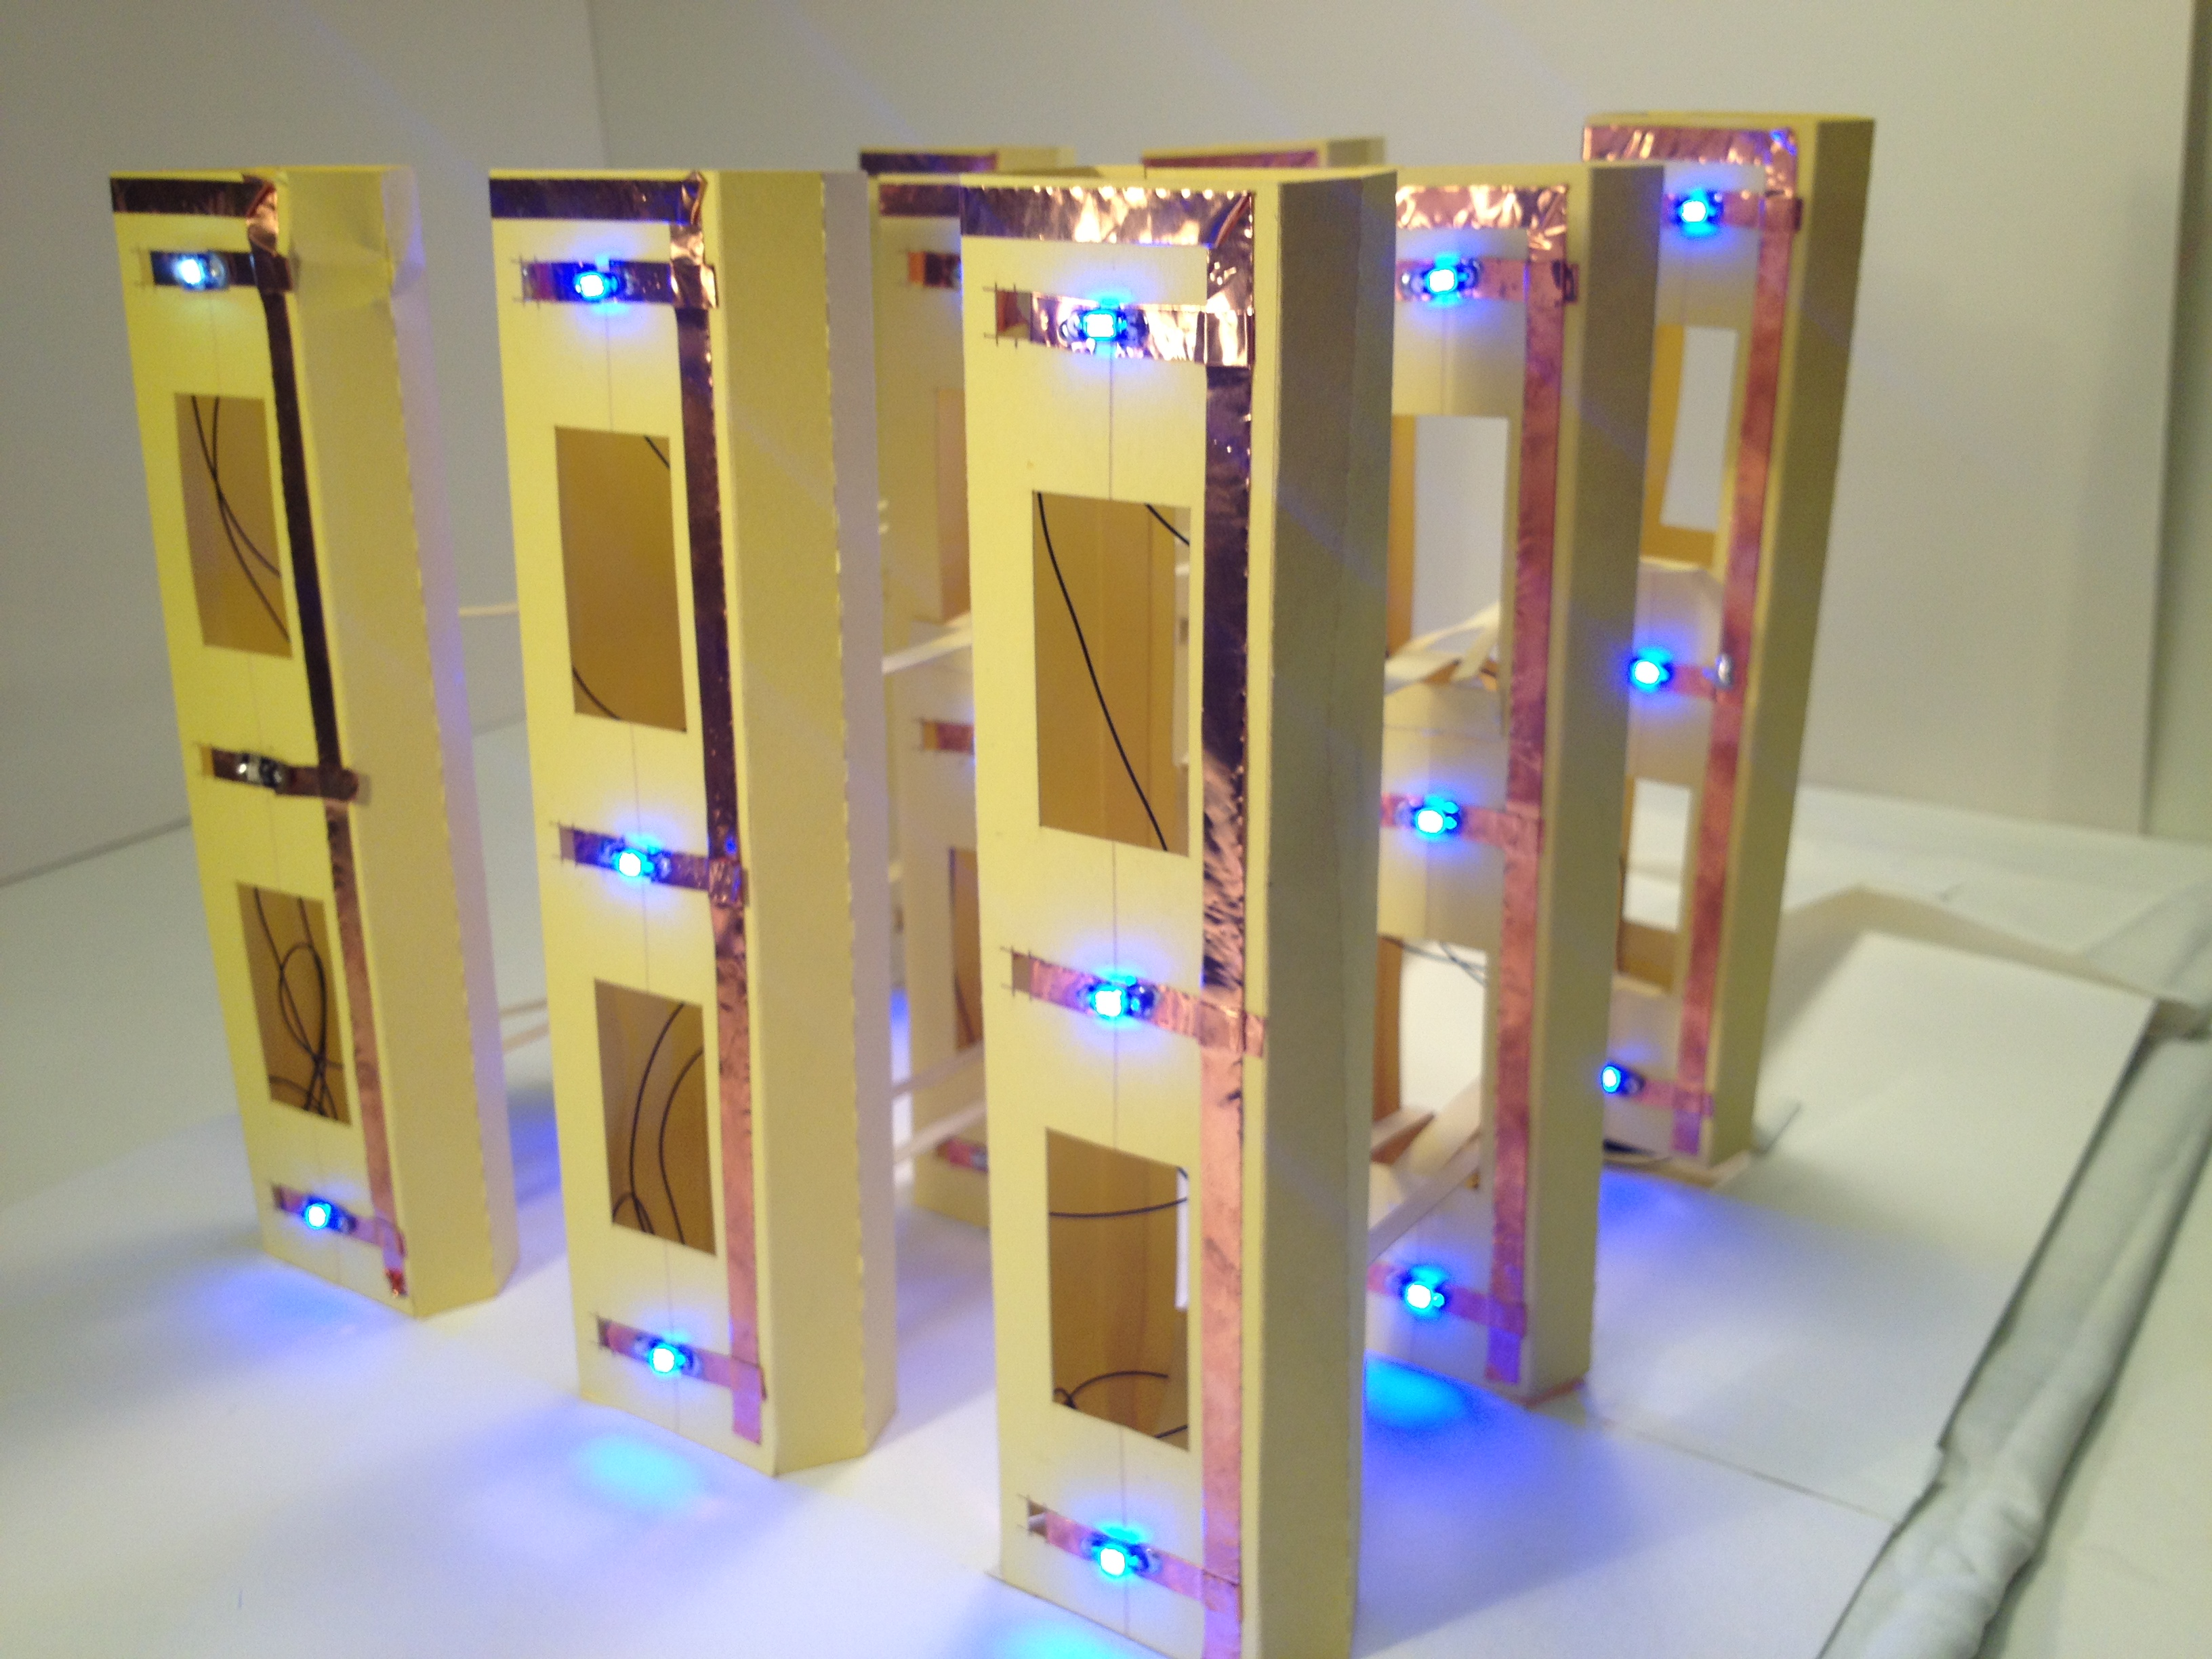
\includegraphics[width=.45\linewidth]{images/popcad25}&
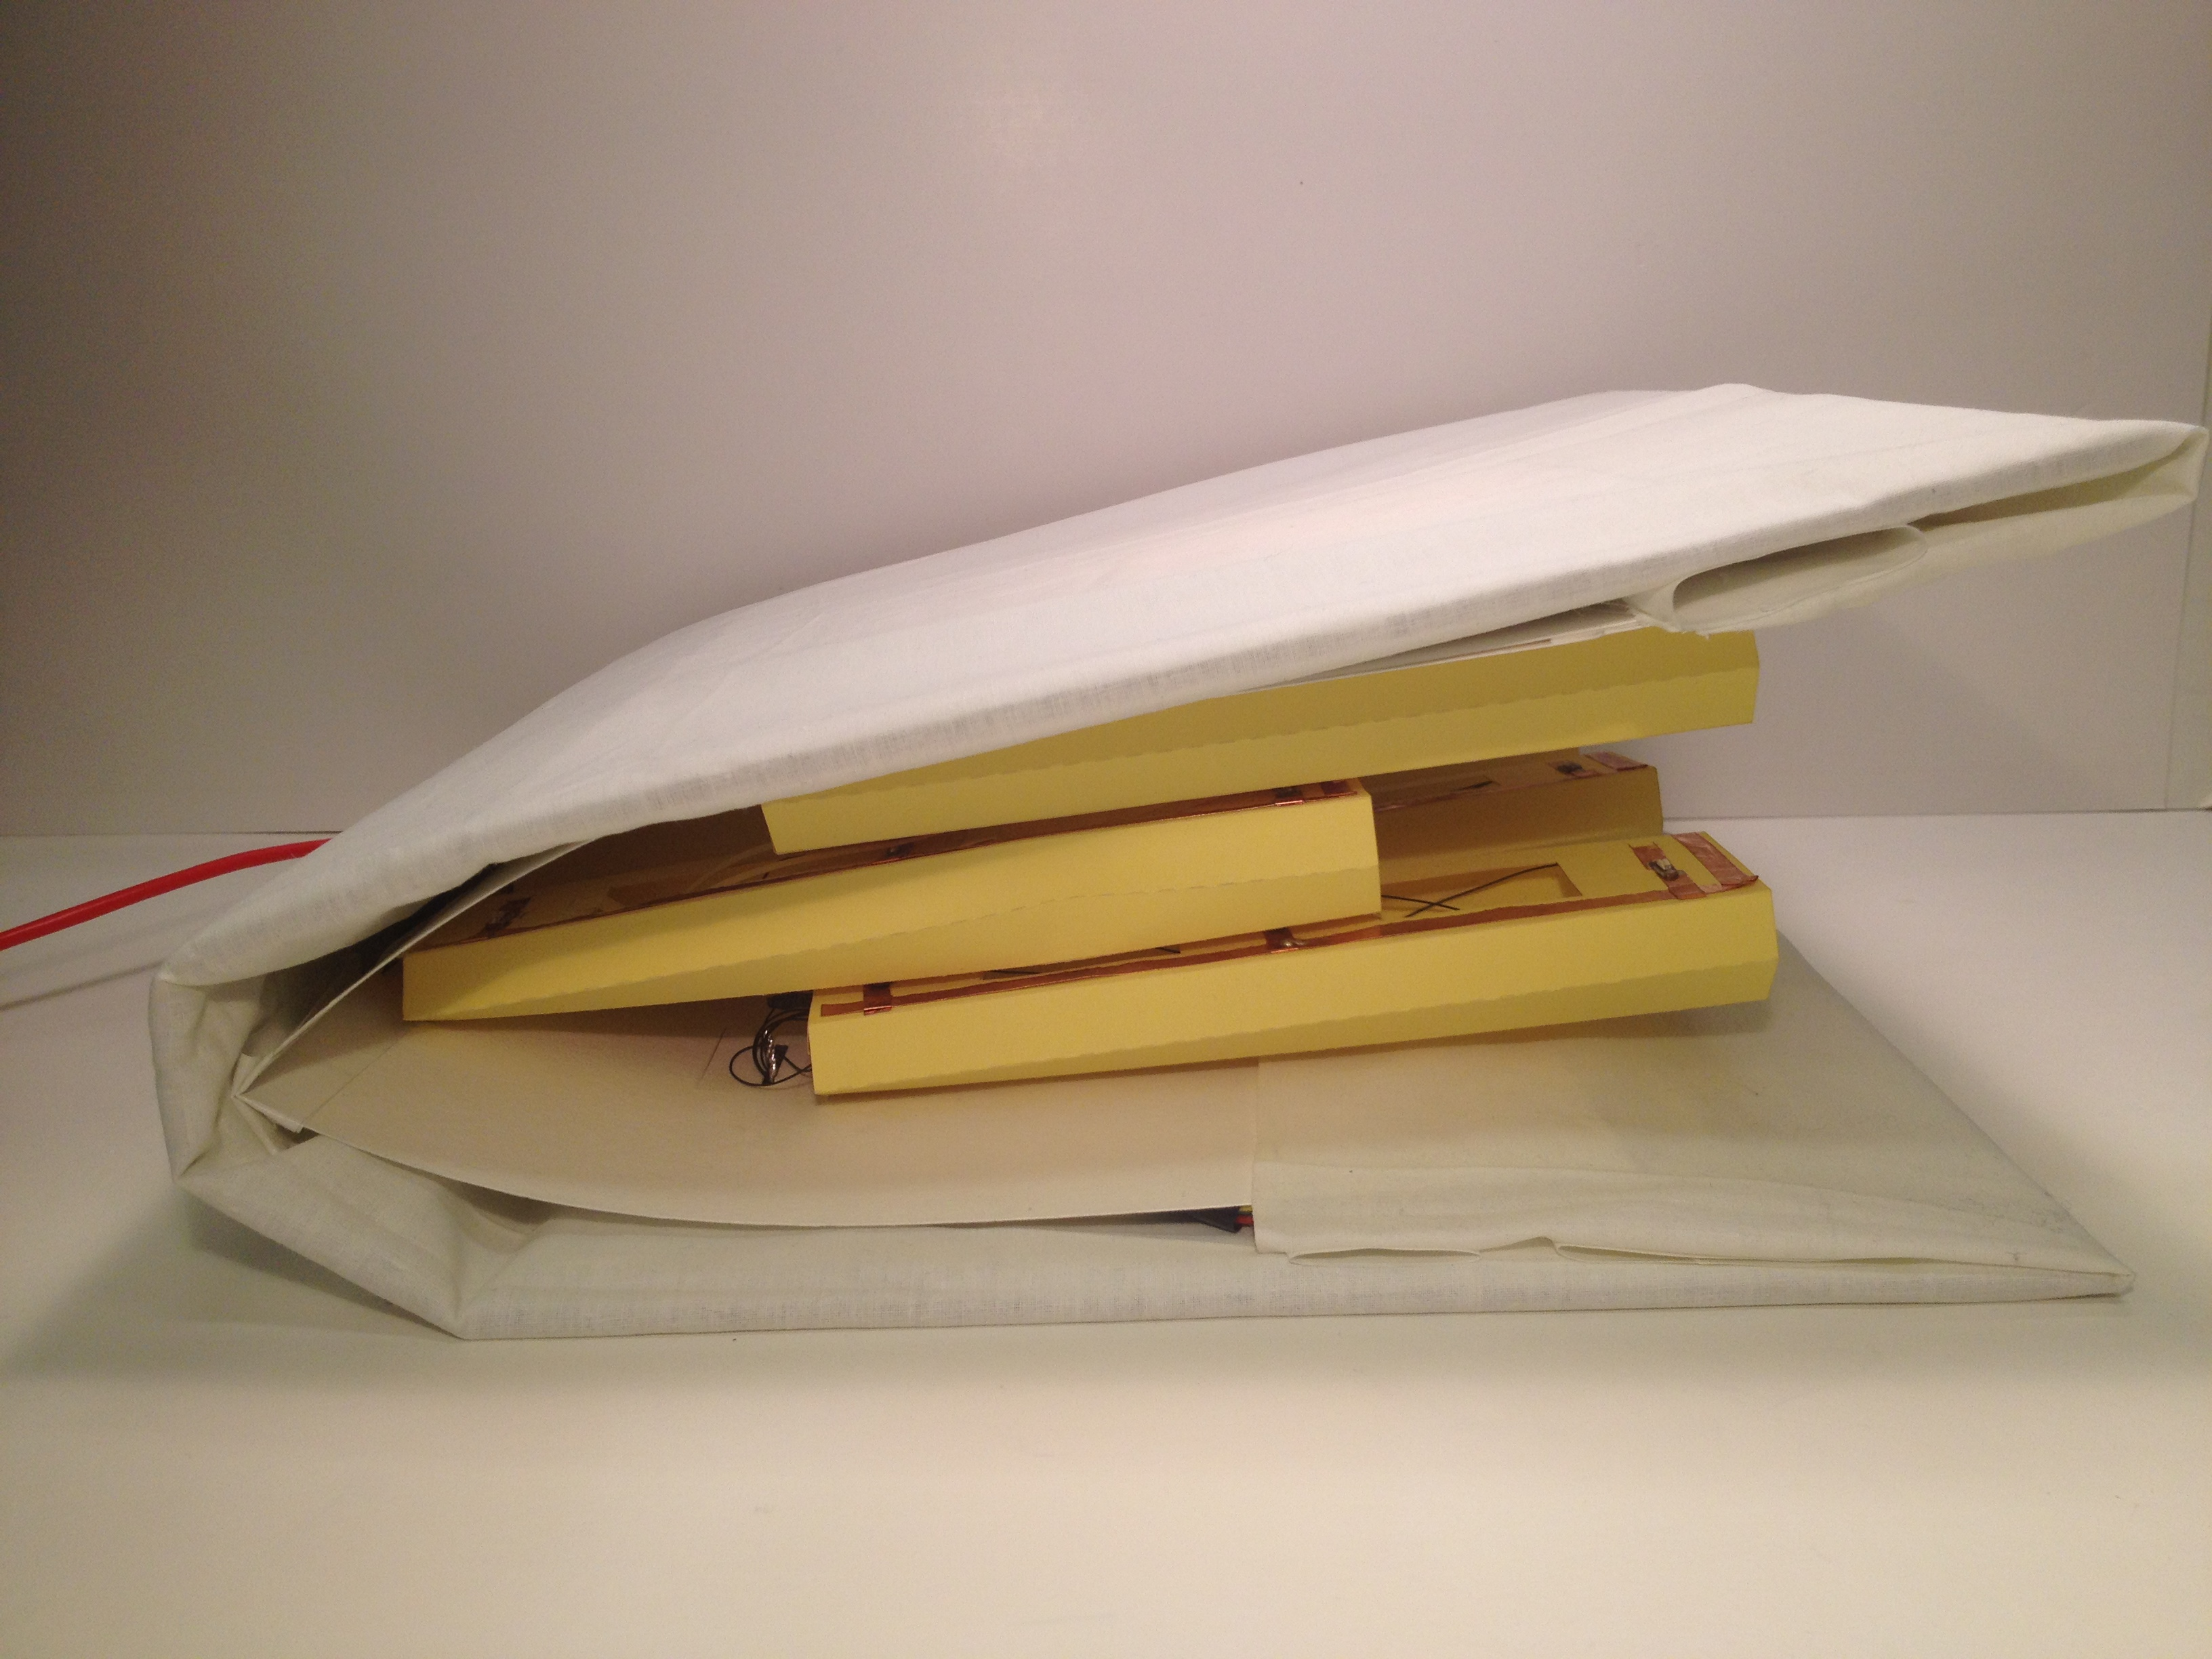
\includegraphics[width=.45\linewidth]{images/popcad44}
\end{array}$
\end{center}
\caption{Two views of the first pop-up book prototype, showing the interface in
both open and closed states.}
\label{fig:popup}
\end{figure}

Each tower has a copper tape circuit consisting of three LEDs on the front face
and three corresponding capacitive touch sensors on the left face. The copper
tape acts as a paper-friendly conductive material to connect the electronic
components together much like traditional wire. The LEDs are soldered onto the
copper tape for greater stability. The capacitive sensors are simply a piece of
copper tape which is connected to a pin on a microcontroller (in the first
version, this is an Arduino Mega Pro). By bringing the internal pull-up resistor
connected to the pin ``LOW'' (to ground) and then timing how long it takes to get
back to a ``HIGH'' state we can tell if the connection is being influenced by a
capacitive force. For example, if there is no interference on the circuit, the
timer will normally only get to ``1'' before the resistor is back to a HIGH state;
if a finger is placed on the copper tape, the reading will be
much higher (typically around ``17''). Based on this change, we can detect which
switch was touched and toggle the associated LED on or off. The hollow interior
of each paper tower is used to solder thin 30-gauge wire to the three LEDs, the
three switches, and ground. These seven wires are soldered to a row of headers
that stick through the bottom of the first layer of the pop-up book. Wires are
then run along the backside of the top layer of paper from these headers to the
microcontroller. The entire circuit in then encased in a cloth-covered cardboard
binder that acts as a book cover as well as a means to protect and hide the
electronics.

\begin{figure}[!ht] \begin{center}$
\begin{array}{cc}
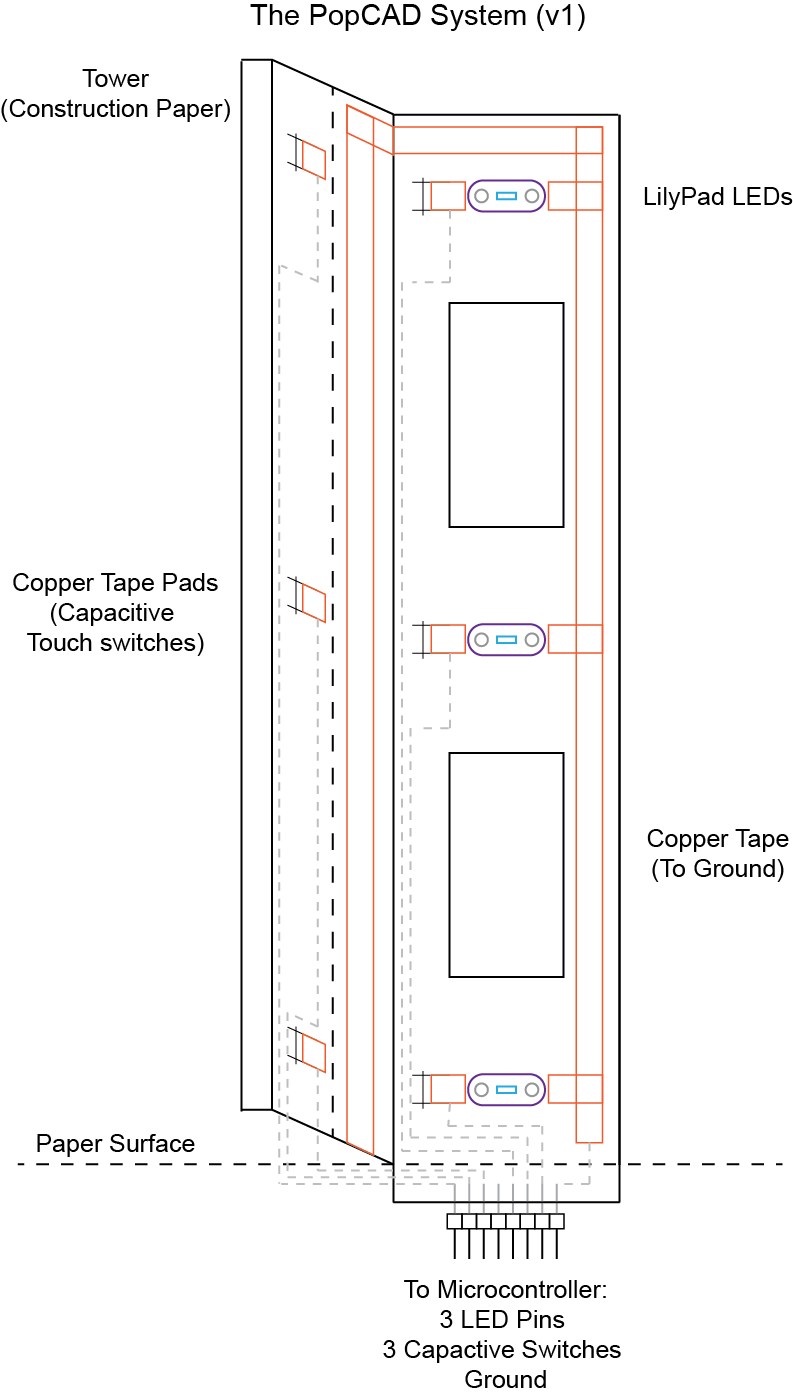
\includegraphics[width=.4\linewidth]{images/PopCadSchematicV1}&
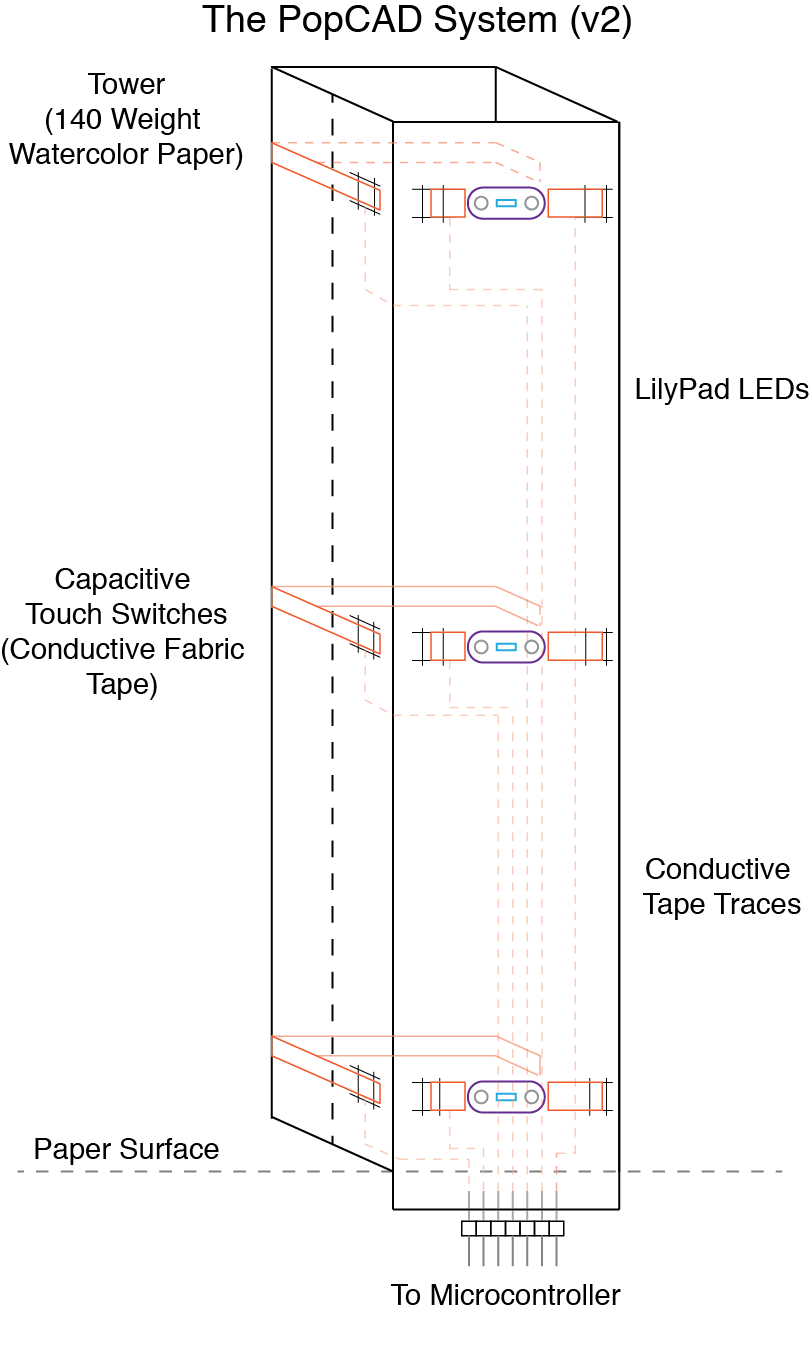
\includegraphics[width=.42\linewidth]{images/PopCadSchematicV2}
\end{array}$
\end{center}
\caption{The two PopCAD designs side-by-side: PopCAD v1 (left) uses copper tape
and 30 gauge wire for the paper circuit, while PopCAD v2 (right) uses
fabric-based conductive tape without needing any wires.}
\label{fig:popup_schematic1}
\end{figure}

\subsection{PopCAD v2}
% 
% This is where we talk about the differences: conductive tape, laser cutting,
% paper choice circuit wiring is more efficient, no horizontal struts\ldots

Although the first PopCAD iteration was a fully-functional prototype, as we
approached user testing with the PopCAD it became apparent that there
were several compelling reasons to iterate on the original design. Through a few
informal user evaluations as well as our own reflections on the device, we
identified several key issues that could be improved upon: (a) the paper
engineering design, (b) the structural integrity of the book as a whole, and (c)
the lack of ``paper-ness'' with respect to the circuitry and electrical
components of the design.

 \begin{figure}[!ht]
  \centering
  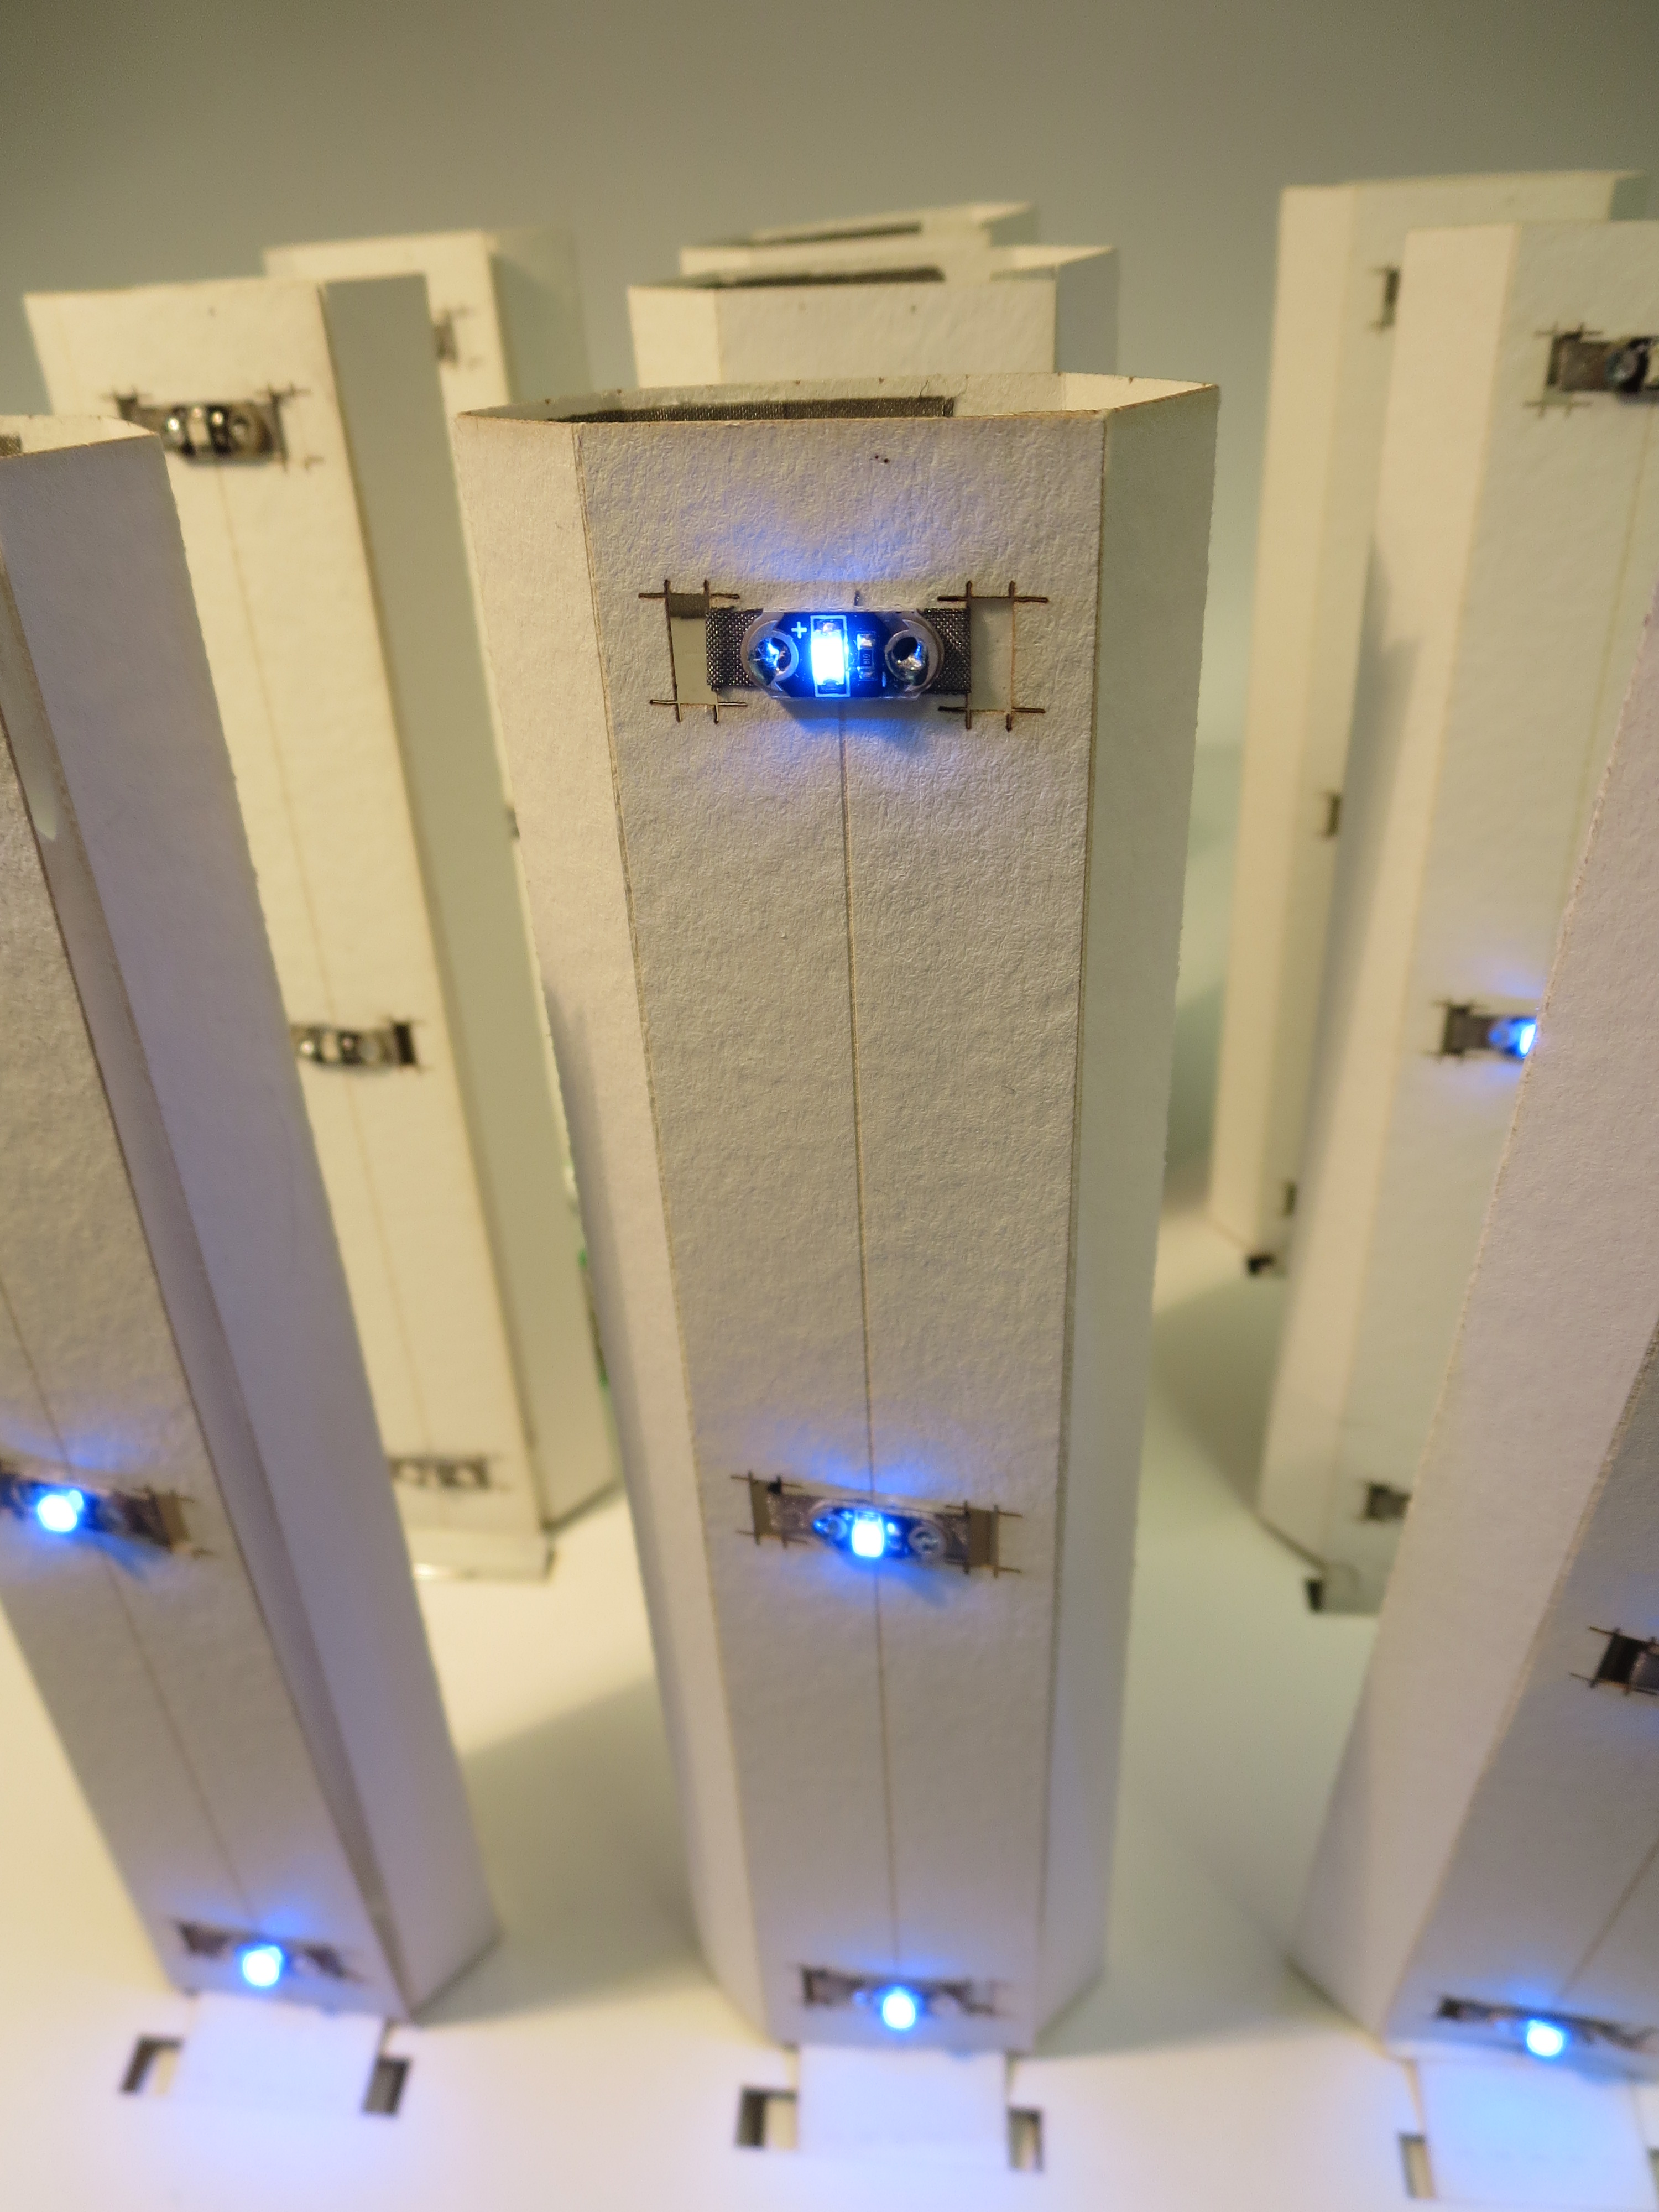
\includegraphics[width=.4\linewidth]{images/pop3}
  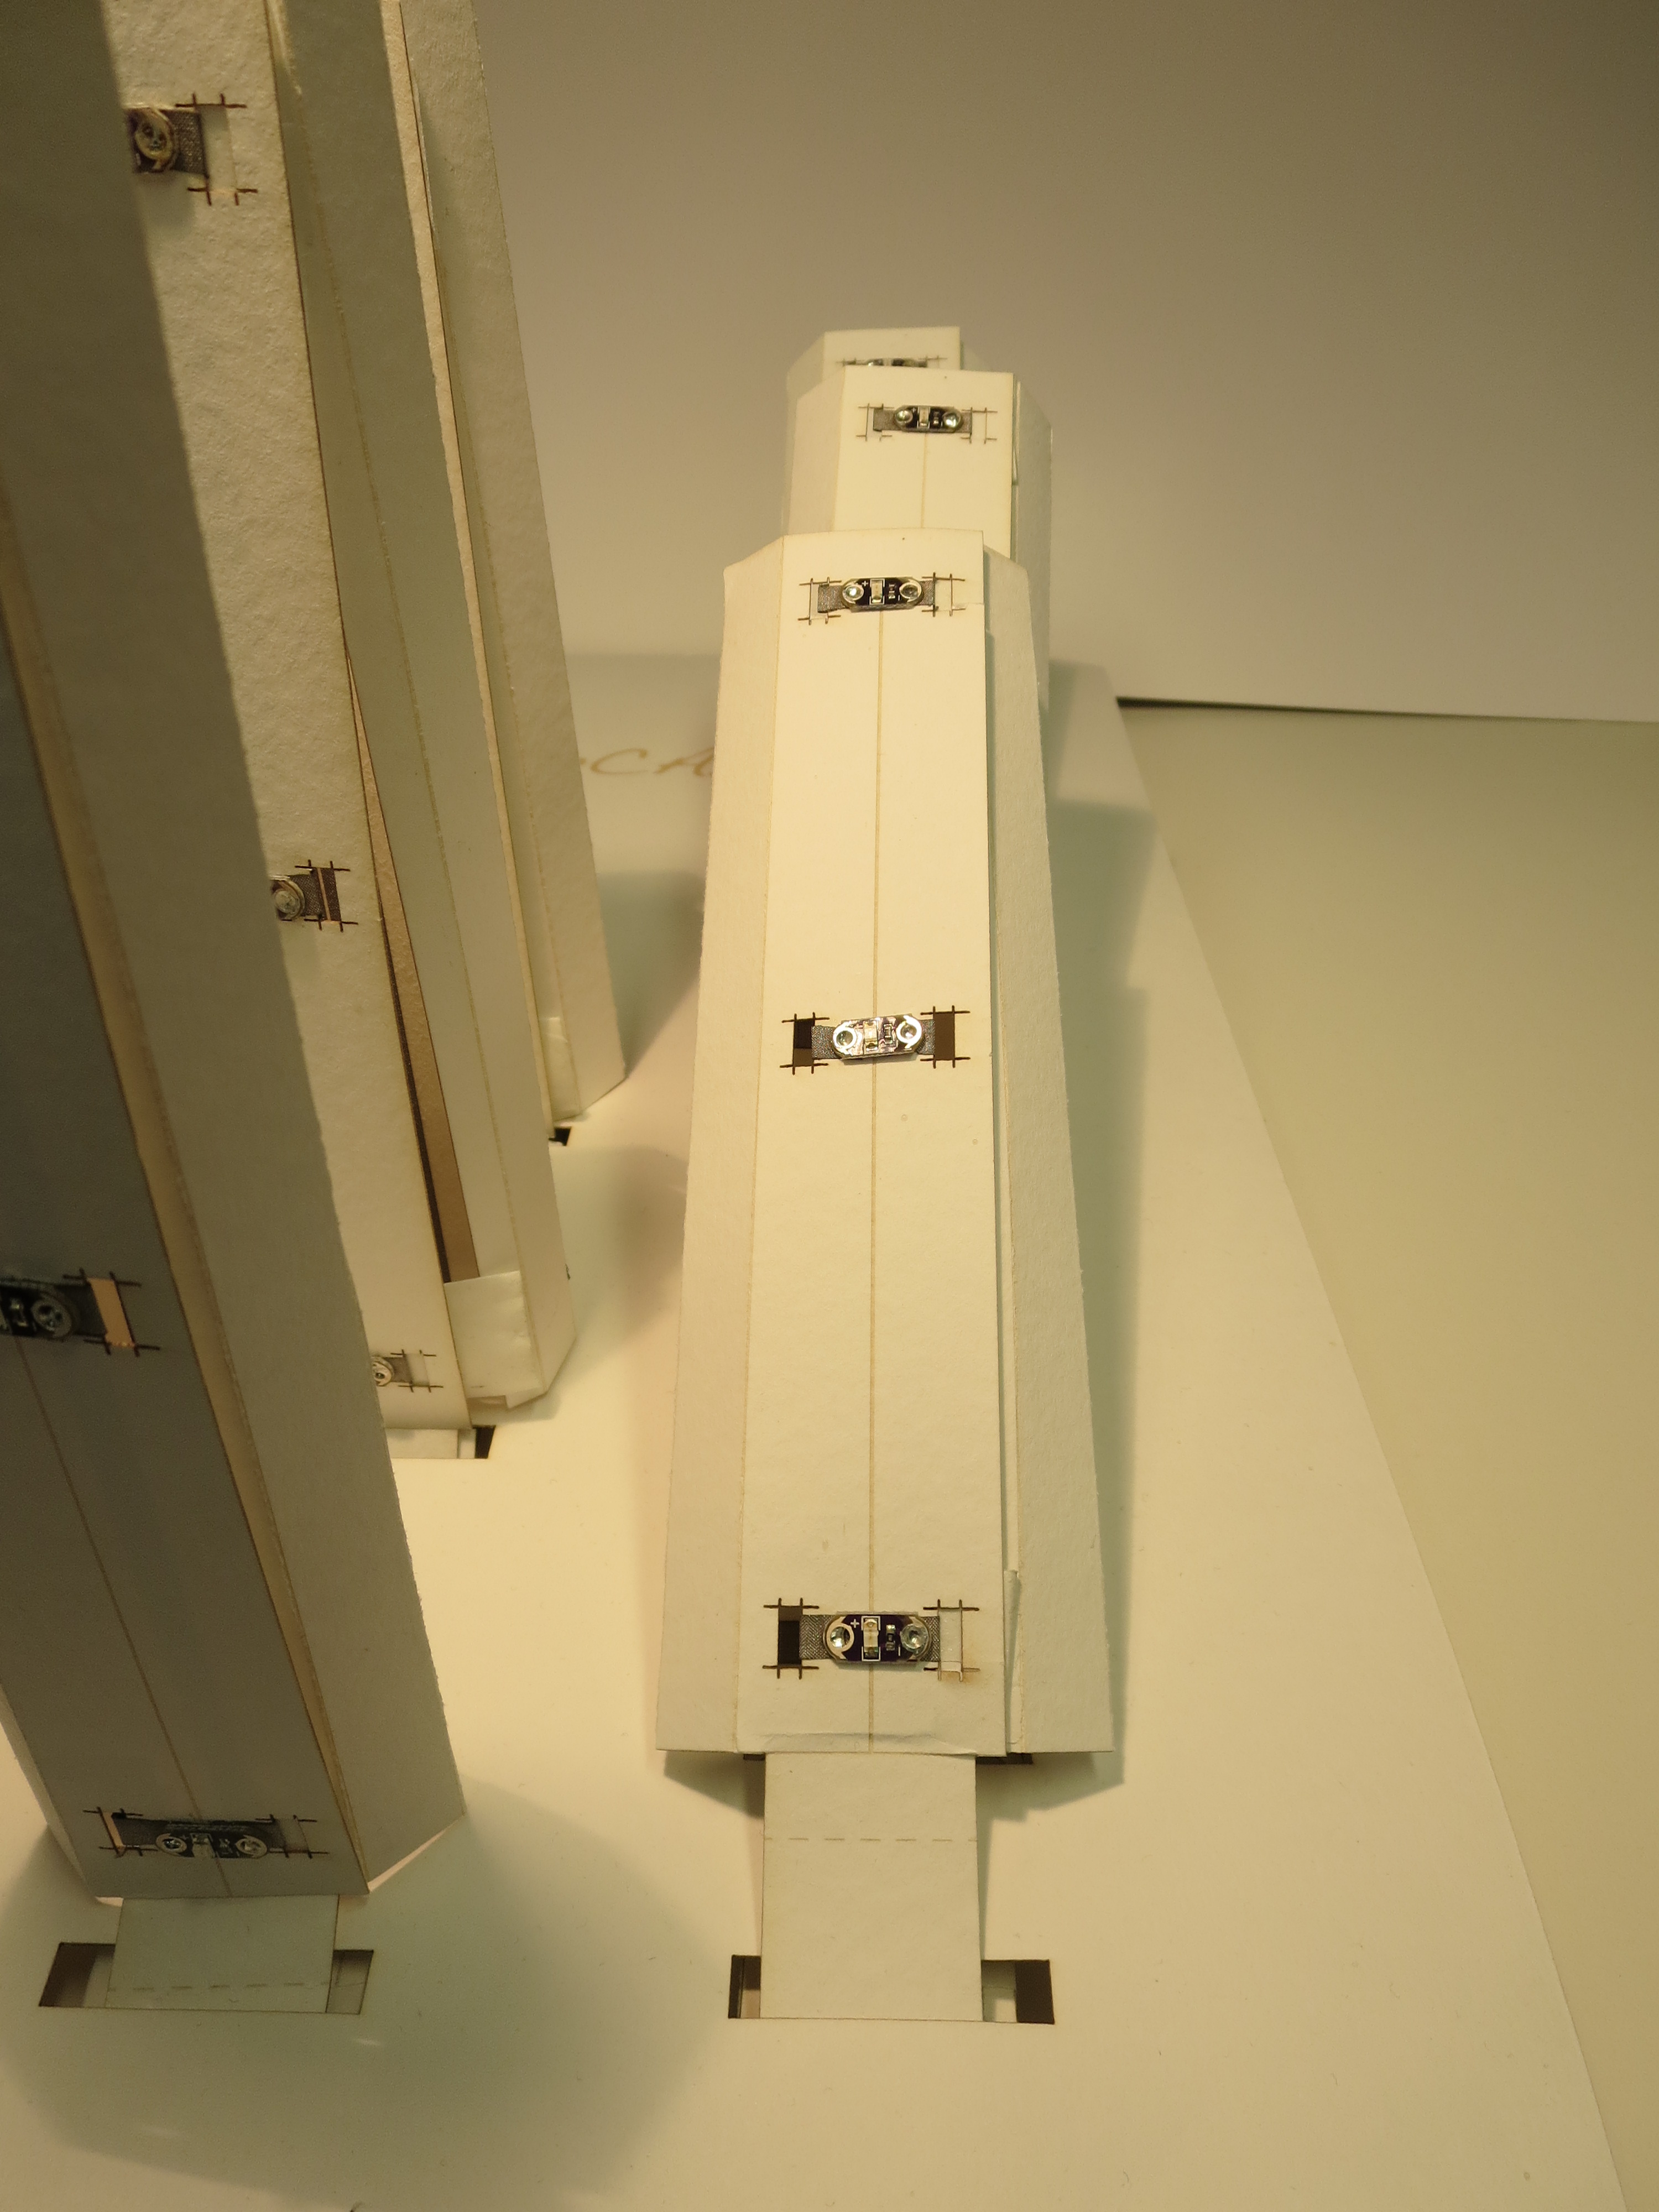
\includegraphics[width=.4\linewidth]{images/popcad_pic2}
  \caption{Two views of PopCADv2 design: with towers raised and LEDs lit
  (left), and with the rightmost column of towers laid flat (right).}
  \label{fig:popcad1}
\end{figure}

To start with the first point above, then: a look at the initial design of the
pop-up mechanism reveals the presence of horizontal paper ``struts'' connecting
the towers in the middle column (along the center crease) to their counterparts
on either side. These struts were necessary in order to generate a pop-up motion
from the middle of a book and force each tower upright. The mechanism was
successful; however, the struts directly interfered with the ability to reach
many of the conductive tape switches. In version two of the PopCAD, the struts
were removed in favor of a pull-tab system whereby each row of towers is raised
and lowered by a tab at the front of the row (the pull tab system can be seen in 
Figure \ref{fig:popcad1}).

We were concerned about the overall stability of the first prototype; lights
would sometimes fail to operate properly, the horizontal struts kept breaking,
parts of the towers were weak, certain points in the wiring were weak, and the
opening and closing of book (and thus the folding of the towers) put enough
strain on the circuitry that we were concerned whether it would survive a user
study. The second prototype addresses these issues in several ways: first, we
use a heavy watercolor paper (140 weight) for all the paper engineering, making
the towers and the pull-tab mechanisms more resilient to repetitive use. Second,
we replace the copper tape, which has a tendency to break over heavy creases,
with conductive fabric tape, which resists repeated creasing much better, and
finally, we made adjustments to lessen the strain on the towers and the
circuitry, by minimizing stress points and reinforcing known weak spots.

\begin{figure}[!ht] 
\begin{center}$
\begin{array}{cc}
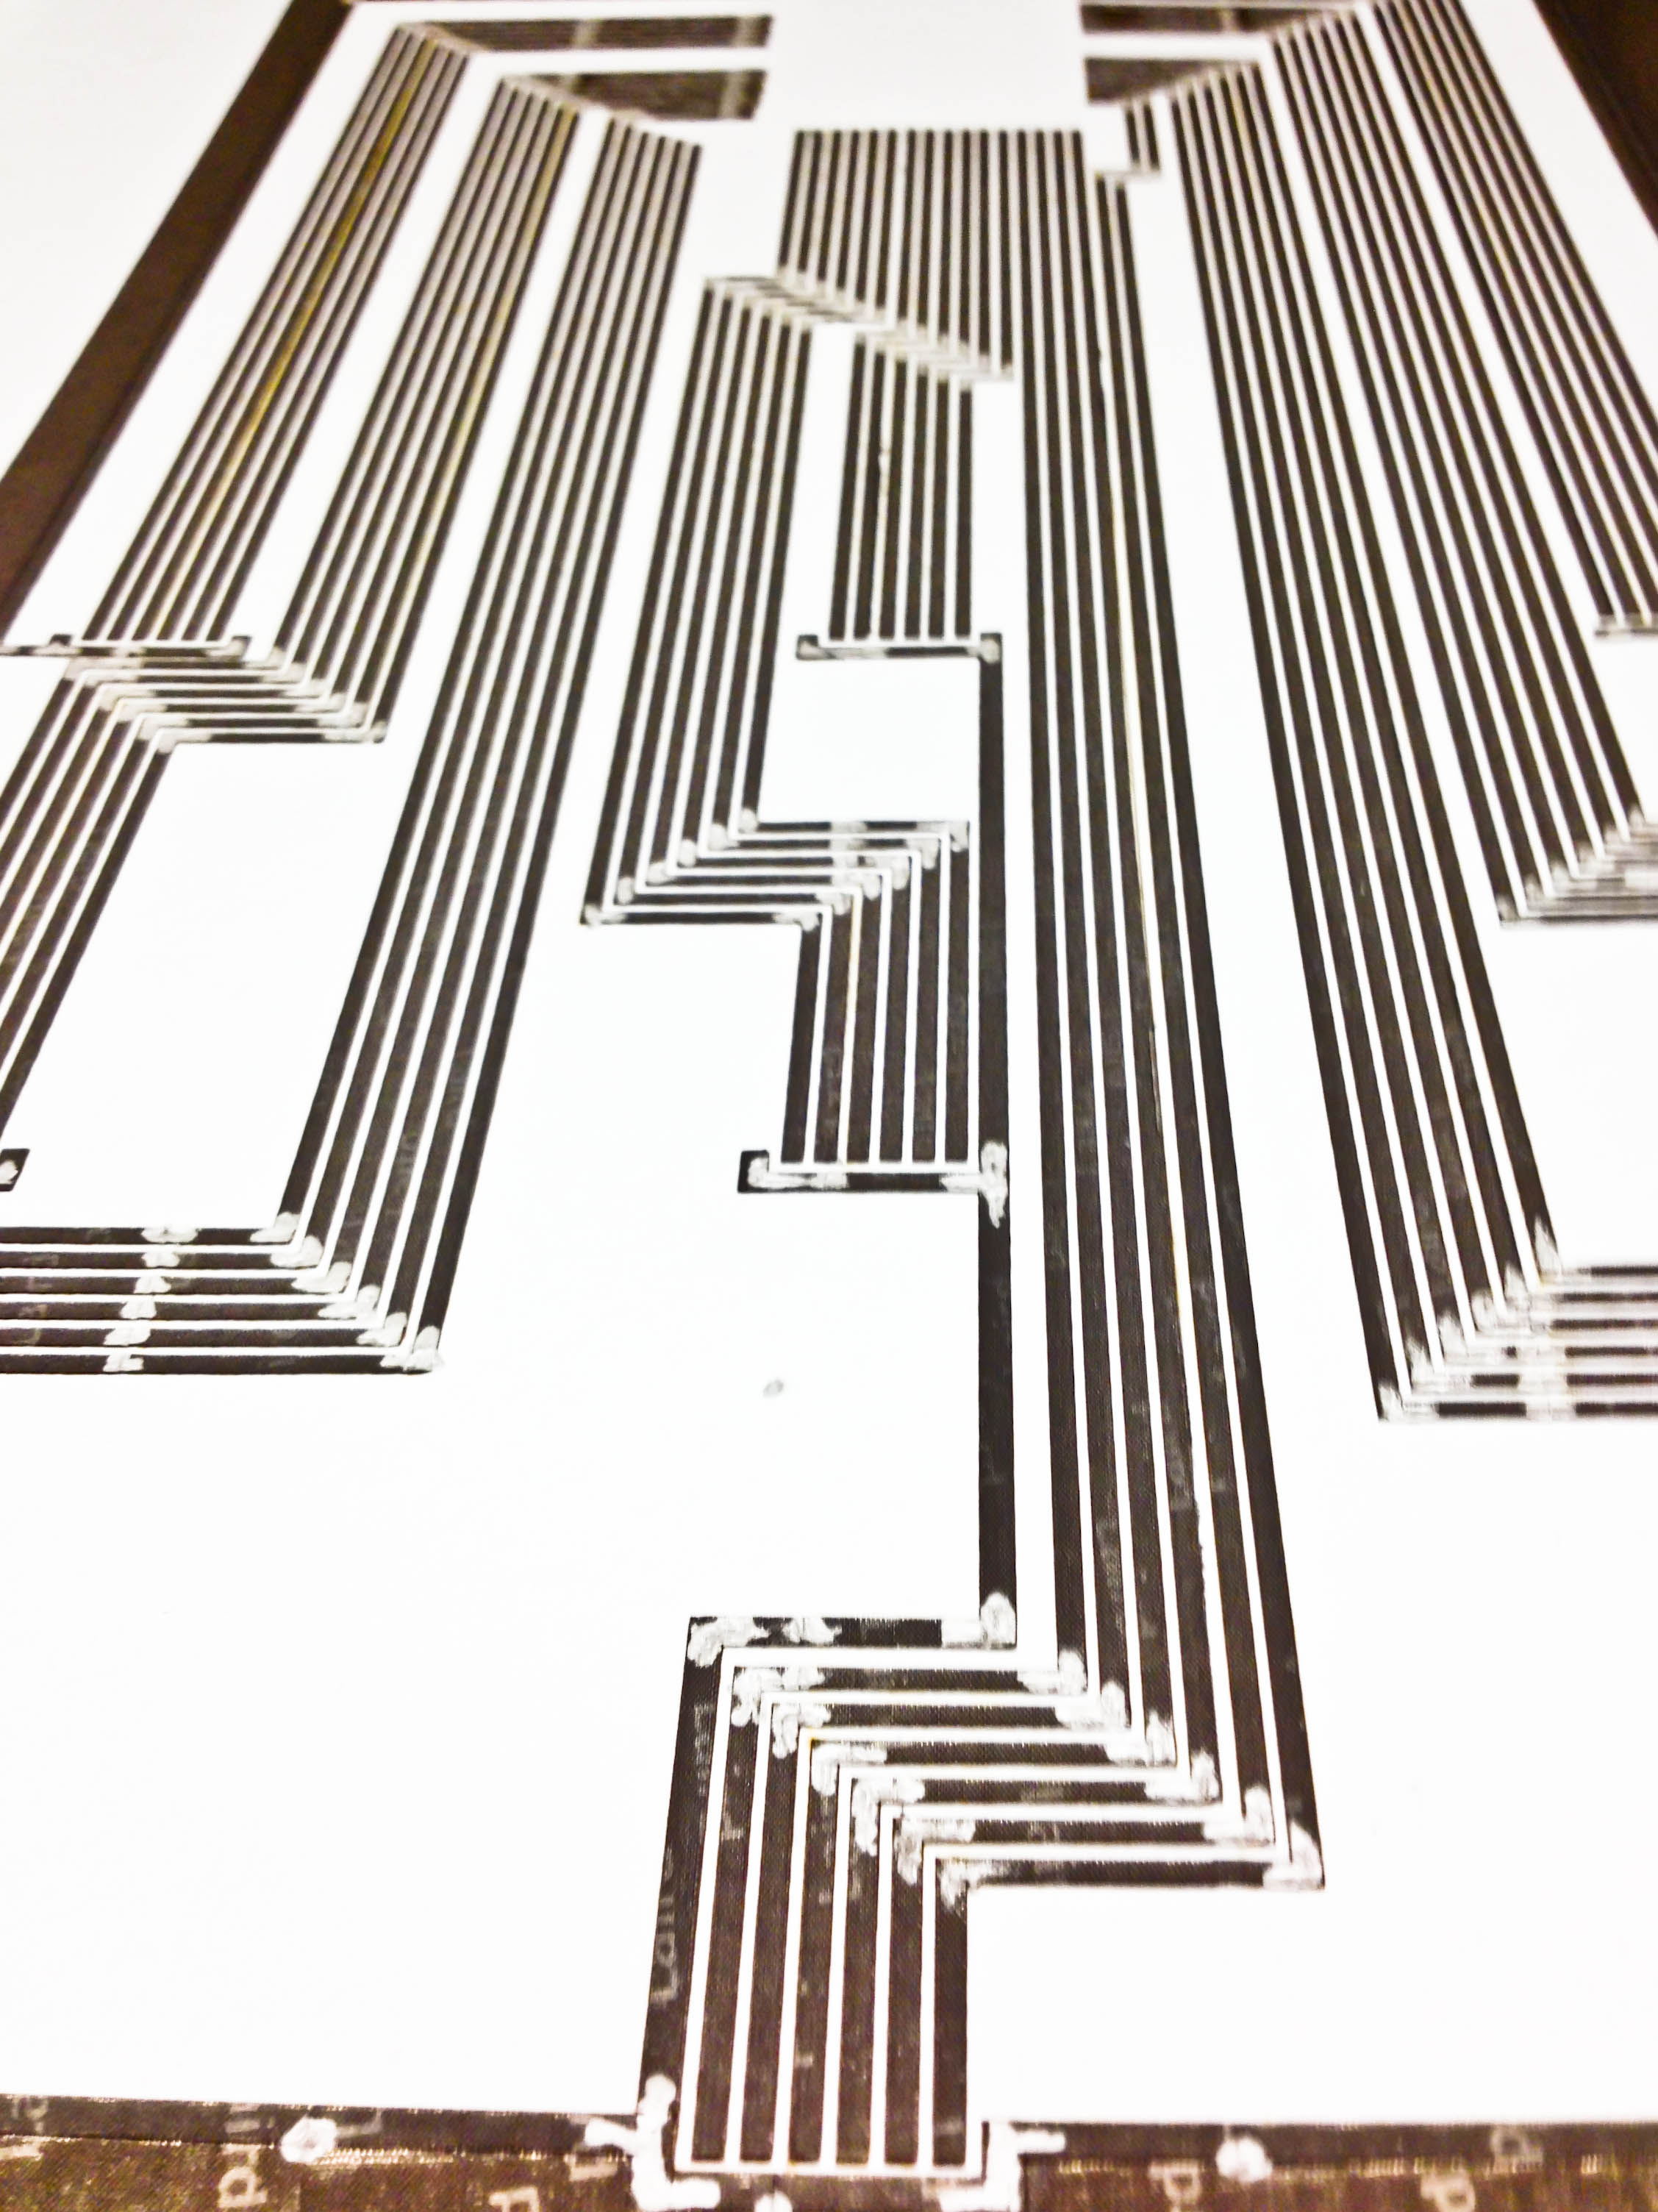
\includegraphics[width=.3\linewidth]{images/pop_circuit2-2}&
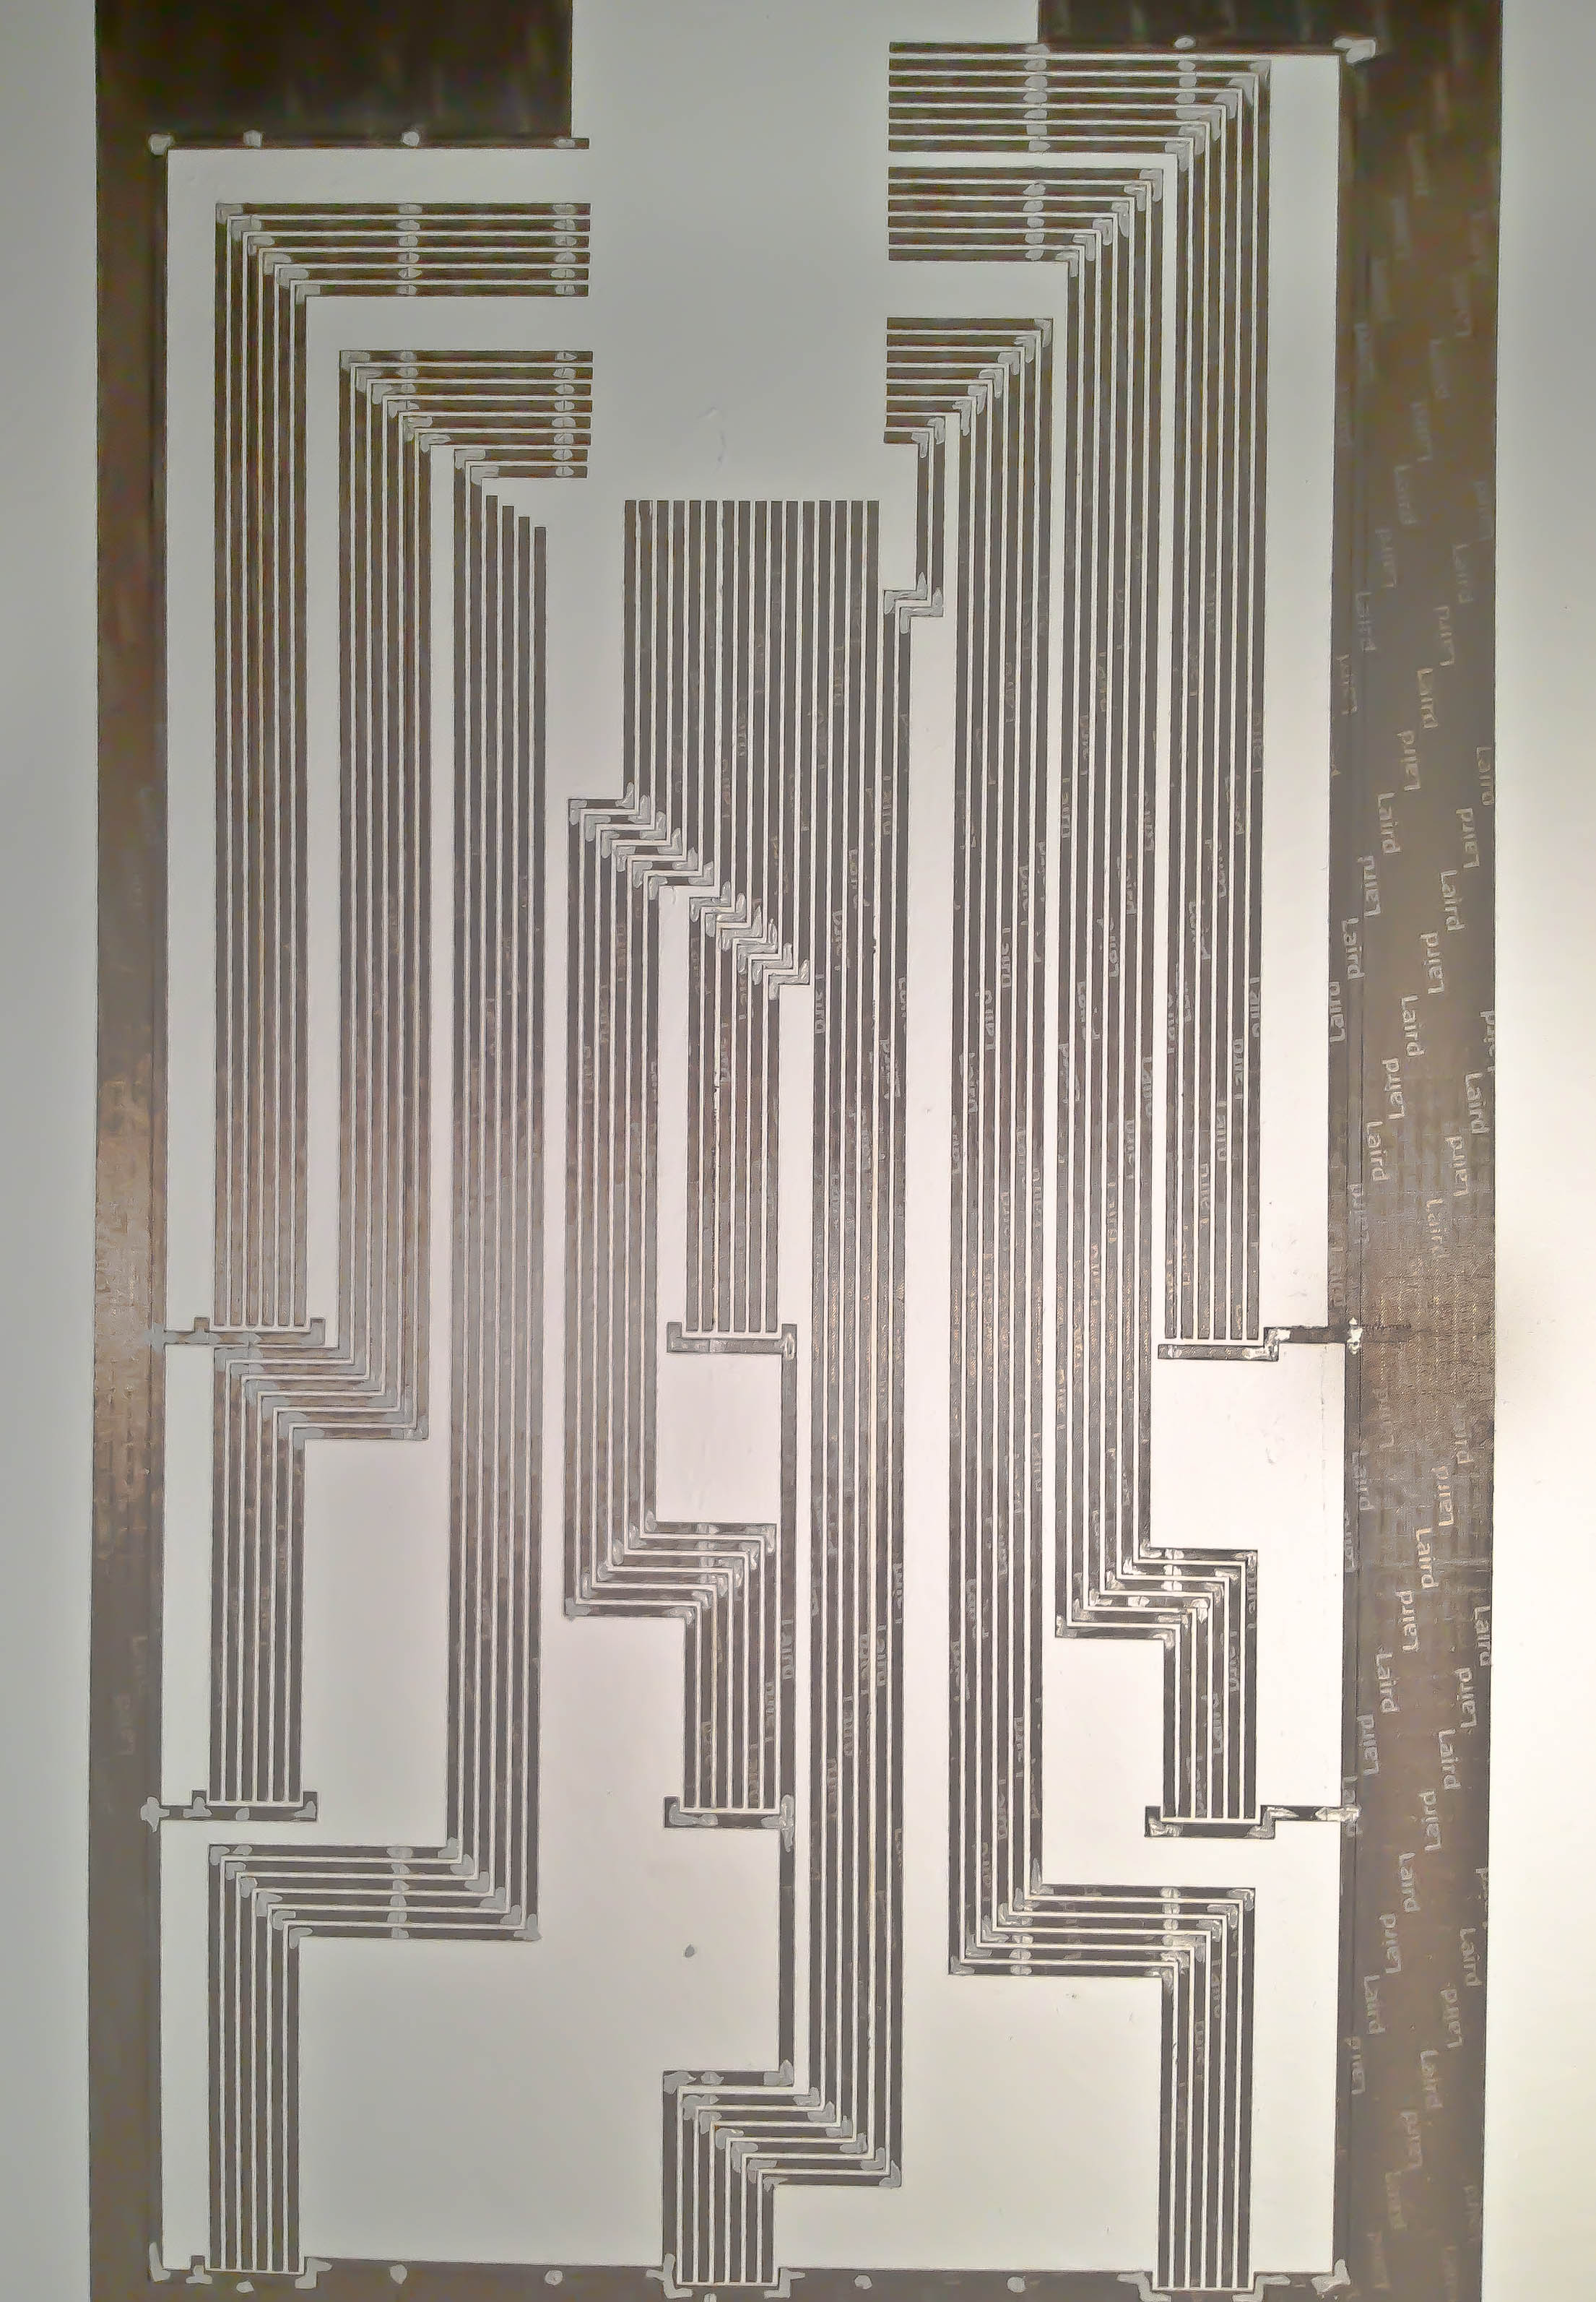
\includegraphics[height=.6\linewidth, angle=90,
width=3.6in]{images/popcad_circuit-3} \end{array}$
\end{center}
\caption{Two views of the conductive tape circuit connecting the paper towers
to the Arduino Mega microntroller. The circuit was constructed by laser cutting
a design through conductive tape (but not through the paper beneath it) and
removing the excess material.}
\label{fig:popcadCirc}
\end{figure}

In the first prototype, we still used traditional jumper wires from the Arduino
to connect to the headers beneath the towers, and 30 gauge (still traditional)
wire inside of the towers to connect from the headers to the LEDs and copper
tape. Admittedly, this does not feel very ``book-like'', or in the spirit of
faithfully exploring paper-based electronics. PopCAD v2 has no traditional
``wires'' at all. Instead, we use a fabric-based conductive tape, which, besides
laying flush (unlike wires) and feeling more like paper than copper tape, the
fabric tape is (unlike copper tape) able to be used in the laser cutter in our
lab. Figure \ref{fig:popcadCirc} shows two views of the PopCAD v2 circuit,
constructed by placing strips of the conductive tape on watercolor paper, laser
etching a circuit diagram through the tape (but not through the paper), and
peeling away the excess. This technique allows us to create a precise yet
completely flat circuit layout. The accuracy of this method permits the Arduino
Pro Mega (a thinner version of the regular Arduino Mega) to be affixed directly
onto the paper. The towers use this conductive fabric for the capacitive touch
sensors as well as material to solder the LEDs to, eliminating all the standard
wires from our design.

The software for the PopCAD retains all the algorithmic capabilities of the
SnapCAD version of the software (convex hull, path, minimal spanning tree), but
as the LEDs are affixed to the towers, we lose the ability for multiple player
functions. However, it should be noted that this was in part intentional; we did
not want any loose parts that could easily break, get lost, or other make the
device less portable. As it stands, the PopCAD (unlike its predecessors) is
self-contained as one piece, is small and light enough to be carried with one
hand, and is considerably less expensive (and less time-consuming) to produce.
We offered sample use cases for the previous devices that involved descriptions
of various technical features; for the PopCAD it seems more appropriate to
instead paint a more general user scenario that speaks to the intent behind
PopCAD's design. Imagine an art teacher, girl scout troop leader, hackerspace or
FabLab member, or any number of educators either wondering how to get into this
``3D printing thing'' or who have a Makerbot sitting in a corner gathering dust.
They find plans online (perhaps on Instructables\cite{Instructables} or some
similar DIY-oriented forum) for a relatively cheap, portable device that they
could not only turn into a group project to build with their kids, but once
built would offer a new way to introduce children to 3D modeling and 3D printing
in a completely new way. The democratization of digital fabrication technology
is (as stated earlier) a core goal of this work, and in many ways the PopCAD is
the device that embodies this ideal the most. So while it may be less expressive
or powerful in some ways (though as we point out in later chapters, this can
sometimes be an advantage), the PopCAD does have a place in our suite of
devices.




% \subsection{Discussion}
%  
% 
% Given the different medium of the pop-up book (paper as opposed to circuit
% boards), it is worth exploring the possibilities afforded by a cheaper, more
% flexible material. For instance, the flexibility of paper might provide the
% means for new types of modeling actions. It is plausible to imagine paper tabs
% or other mechanisms that perturb the LEDs off the integer lattice, or alter the
% overall topology in such a way that new shapes are possible (e.g. by deforming
% an equidistant grid into a spherical shape). There may be additional sensors or
% hardware that could be embedded into the book to provide new functionality
% (rotation, proximity, pressure). Additionally, due the inexpensive and portable
% nature of the pop-up book, it is worth exploring the sorts of interactions that
% could occur between several pop-up books (e.g., extending the input field to
% include two or more grids, networked interactions like cooperative modeling
% tasks, or competitive games like 3D-battleship). By using paper as a material to
% think with, we may find further possibilities as development continues.

\section{Software}
% \subsection{Software}
% 
% The UCube makes use of the Processing\cite{Processing} framework to read in
% the active coordinates from the Arduino microcontroller connected to the
% platform; the software then displays these as larger red points on a grid of
% grey dots. Users can rotate the grid along any axis by clicking and dragging
% with the mouse. In our current early prototype, there are only two buttons on
% the user interface: (i) an �export� button, responsible for taking the current
% set of active points and exporting them into "STL" file format (suitable for 3D
% printers), and (ii) a �mode� button which toggles between showing just the red
% dots as points and filling in an area (defined by a convex hull algorithm) to
% give a sense of shape.
% The software interface is intentionally minimal in order to encourage the user
% to focus on the physical interaction. We felt it was crucial not to fall into
% the trap of making another software tool for experts, so the main purpose of the
% software is to act as an aid�a means to cognitively clarify and confirm the
% user's intentions. Although it is likely that we will extend the software
% somewhat in future iterations, our goal is to support the physical experience of
% specifying a three-dimensional object, and not to add functionality beyond what
% is necessary or helpful to that end.

The software for the aforementioned devices utilizes the Processing Serial
library to read in the active coordinates from an Arduino microcontroller; it
then displays those coordinates on-screen as larger points against a ``ghosted''
grid of grey dots. The exact methods used to achieve this varied by device, and
were detailed in the device-specific sections above. This on-screen model can be
manipulated in a number of ways. Clicking and dragging along any axis rotates
the model, as does the use of the arrow keys on the keyboard.  Holding the shift
key while performing either action moves the entire model around the screen
(essentially re-centering it). The ``control'' key plus an up or down arrow key
zooms in or out along the z-axis. In addition to camera movements, there are a
limited number of functions represented by a simple graphical user interface
which aid and expand the modeling capabilities of the connected device.

For a brief overview of these functions, then: there are three ways of
interpreting the active set of points on the connected device: by taking the
convex hull of the input set, by connecting each point sequentially with a 3D
path, and by connecting the set according to a minimal spanning tree algorithm
(more on these modes soon). There is a single ``export'' button that will take
whatever the active shape is, no matter the mode (if there is one) and generate
a stereolithography file (.STL), the standard file format for 3D printing,
although .STL files can also be opened by more sophisticated 3D modeling
software, providing the possibility for the software to be used as a sort of
``sketchpad'' for rough ideas or shape that can refined afterwards. There is a
``close path'' button which will connect the first and last segments in an open
path (e.g. in constructing a square path, after the fourth point has been
placed, there will still be an open side of the square - pressing this button
will complete the square). There is an ``edit'' mode, whereby the real-time
input from the device is suspended in favor of being able to click-and-drag the
active points around with the mouse. Consequently, there is a reset button, in
the case that the user wishes to ``snap back'' to the normalized integer
lattice. There is also a slider element entitled ``path width'' that will
dynamically adjust each segment or branch width when in path or tree mode,
making the segments ``skinnier'' or ``fatter''. Finally, two minor aesthetic
options - the ``wireframe'' button will turn off the ``fill'' of the shape,
showing the outline stroke with a transparent fill, while the ``grid'' button
will toggle the visibility of the ghosted grid of non-active points.

% There are toggles for turning on and off the convex hull of the active points
% (either all the points or just the hull of a particular color), viewing the hull
% as a wireframe or solid object, and a toggle that shows or hides the background
% grid.  In addition, there are several import and export buttons: an export to
% STL (stereo lithography) format, the standard format for 3D printer files, as
% well as save and load options which allow users to save and re-load their shapes
% for use within the UCube system. Figure \ref{fig:software1} shows the UCube
% software upon reading in the eight points that were selected in Figure 1: in the
% bottom panel, the ``convex hull'' option has been chosen so that a solid cube is
% displayed (with the input points visible as the highlighted vertices of the
% cube). Now, by exporting this form (as mentioned above) to STL format, and
% sending the result to a 3D printer, we can produce a physical model of our
% specified shape, as shown in Figure 4.





% Before returning to the software itself, it is worth pointing out that, in
% effect, the events depicted in Figures 1, 3, and 4 constitute a typical scenario
% for employing the UCube. The user begins by selecting the vertices of a shape
% that she wishes to create (Figure 1); checks that shape against its appearance
% on the computer screen (Figure 3); and, if satisfied, sends that shape on to be
% output by a 3D printing device (Figure 4). There are, of course, limitations to
% this scenario - and we will touch upon these in the ensuing discussion.
% Nonetheless, it is the overall simplicity of the scenario that originally
% inspired the design of the UCube: the user need not construct a shape on a
% two-dimensional screen, nor be deeply familiar with the terminology and
% operations of modeling software. Instead, the creation of a desired shape takes
% place by moving one's hands in space.

As a guiding heuristic for our software design, it should be noted that the
device software is intentionally minimal. Our aim is not to produce another
sophisticated software modeling program - there are plenty of good ones
available already. Instead, the software is meant to aid the user in clarifying
their physical actions with the physical device, while maintaining a low barrier
to entry, a great possibility of expressiveness, and multiple ways of
approaching any given exercise - a trifecta of design heuristics often referred
to by Resnick (and others) as low floors, high ceilings, and wide
walls\cite{Resnick}.

\subsection{Modeling Modes} 

This section will describe the three main modeling modes of the software, with
particular attention to explaining the methods by which they form shapes, the
algorithms behind how they operate, and the modeling domains for which they are
particularly suited.

\subsubsection{Convex Hull: Creating Polyhedral Forms} 

In observing a set of lights placed on an integer lattice in 3-space, one of the
first mental images we thought of was to take the convex hull of that set and
create a solid polyhedral form. One may think of the 2-dimensional convex hull
as the operation performed on the 2D geoboard mentioned earlier in the chapter;
given a randomly scattered set of nails in a board, the convex hull of those
nails will be equivalent to a rubber band that stretched around all the points.
That is, the minimal form that includes all of the line segments connecting each
pair of points, as the rubber band forms a straight line between those nails on
the hull as opposed to curving inward (thus the minimal shape of line segments
as opposed to area). In three dimensions, this becomes a convex polyhedron
instead. Many popular 2-dimensional convex hull algorithms originated in the
early 1970's (e.g. Jarvis March/Gift Wrapping, Graham Scan), while a
3-dimensional solution was published in 1977\cite{preparata1977convex} and
popularized by the same author in the book, \emph{Computational Geometry: An
Introduction}\cite{preparatat1985computational}.

The version implemented in our program is a derivative of the work presented in
\cite{barber1996quickhull}, and adapted from the implementation at \cite{quickhull3d}
which combines a 2D Quickhull Algorithm with a general dimension Beneath-Beyond
Algorithm to achieve a general dimension convex hull solution. In brief, the
strategy works as follows: (a) from a given set of input points, where the
coordinates are known, create an initial 3-simplex (tetrahedron) - from the
min/max points in along each dimension (x,y, and z), and add the four faces of
the tetrahedron to the stack, (b) Pop a face from the stack and get the point
most distant to that face, (c) Find all faces adjacent to the selected face,
find the horizon edges of the adjunct faces and extrude the shape along those
edges to the selected point. (d) Put the newly discovered faces on the stack and
repeat from (b) until all points have been accounted for.

When the hull mode is active in the software, the coordinates on the connected
device must be sent to the hull construction methods each time a point is added
or removed to ensure that the hull remains accurate in real-time. The worst case
for this algorithm is $\Omega(n^2)$, although in practice is not worse than
$\Omega(n$ $log$ $n)$. Figure \ref{fig:software1} shows two screenshots of a
``before and after'' convex hull computation in the software in which the
picture on the left in simply displaying the active set of points, while the
figure on the right shows the interpretation of those points after clicking the
convex hull button.


\begin{figure}[ht] \begin{center}$
\begin{array}{cc}
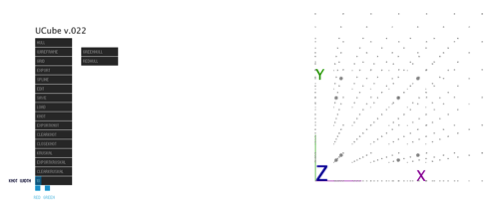
\includegraphics[width=.47\linewidth]{images/software_1} &
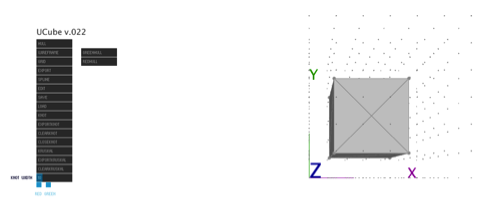
\includegraphics[width=.47\linewidth]{images/software_2}
\end{array}$
\end{center}
\caption{Two screen views (left and right) of the device software, illustrating
the way in which the software displays the convex hull of a cube. Left: The set
of eight input points, before the ``Hull'' button has been pressed. Right: The
resulting convex hull, forming a cube from the input points.}
\label{fig:software1}
\end{figure}

Polyhedral forms obviously have a long history not only in modeling, but in
geometry (the Platonic solids), architecture (the Pyramids of Egypt), and
numerous other disciplines over the ages (building blocks, paper crafts, etc.).
Though not all the Platonic solids can be modeled naturally (i.e. without edit
mode) on our devices, certainly pyramids can be, as well as other common convex
polyhedral shapes (e.g. a canonical ``house'' consisting of a cube with a
tetrahedron sharing the cube's top face). Some examples are shown in Figure
\ref{fig:hulls} below.

\begin{figure}[ht]
\begin{center}
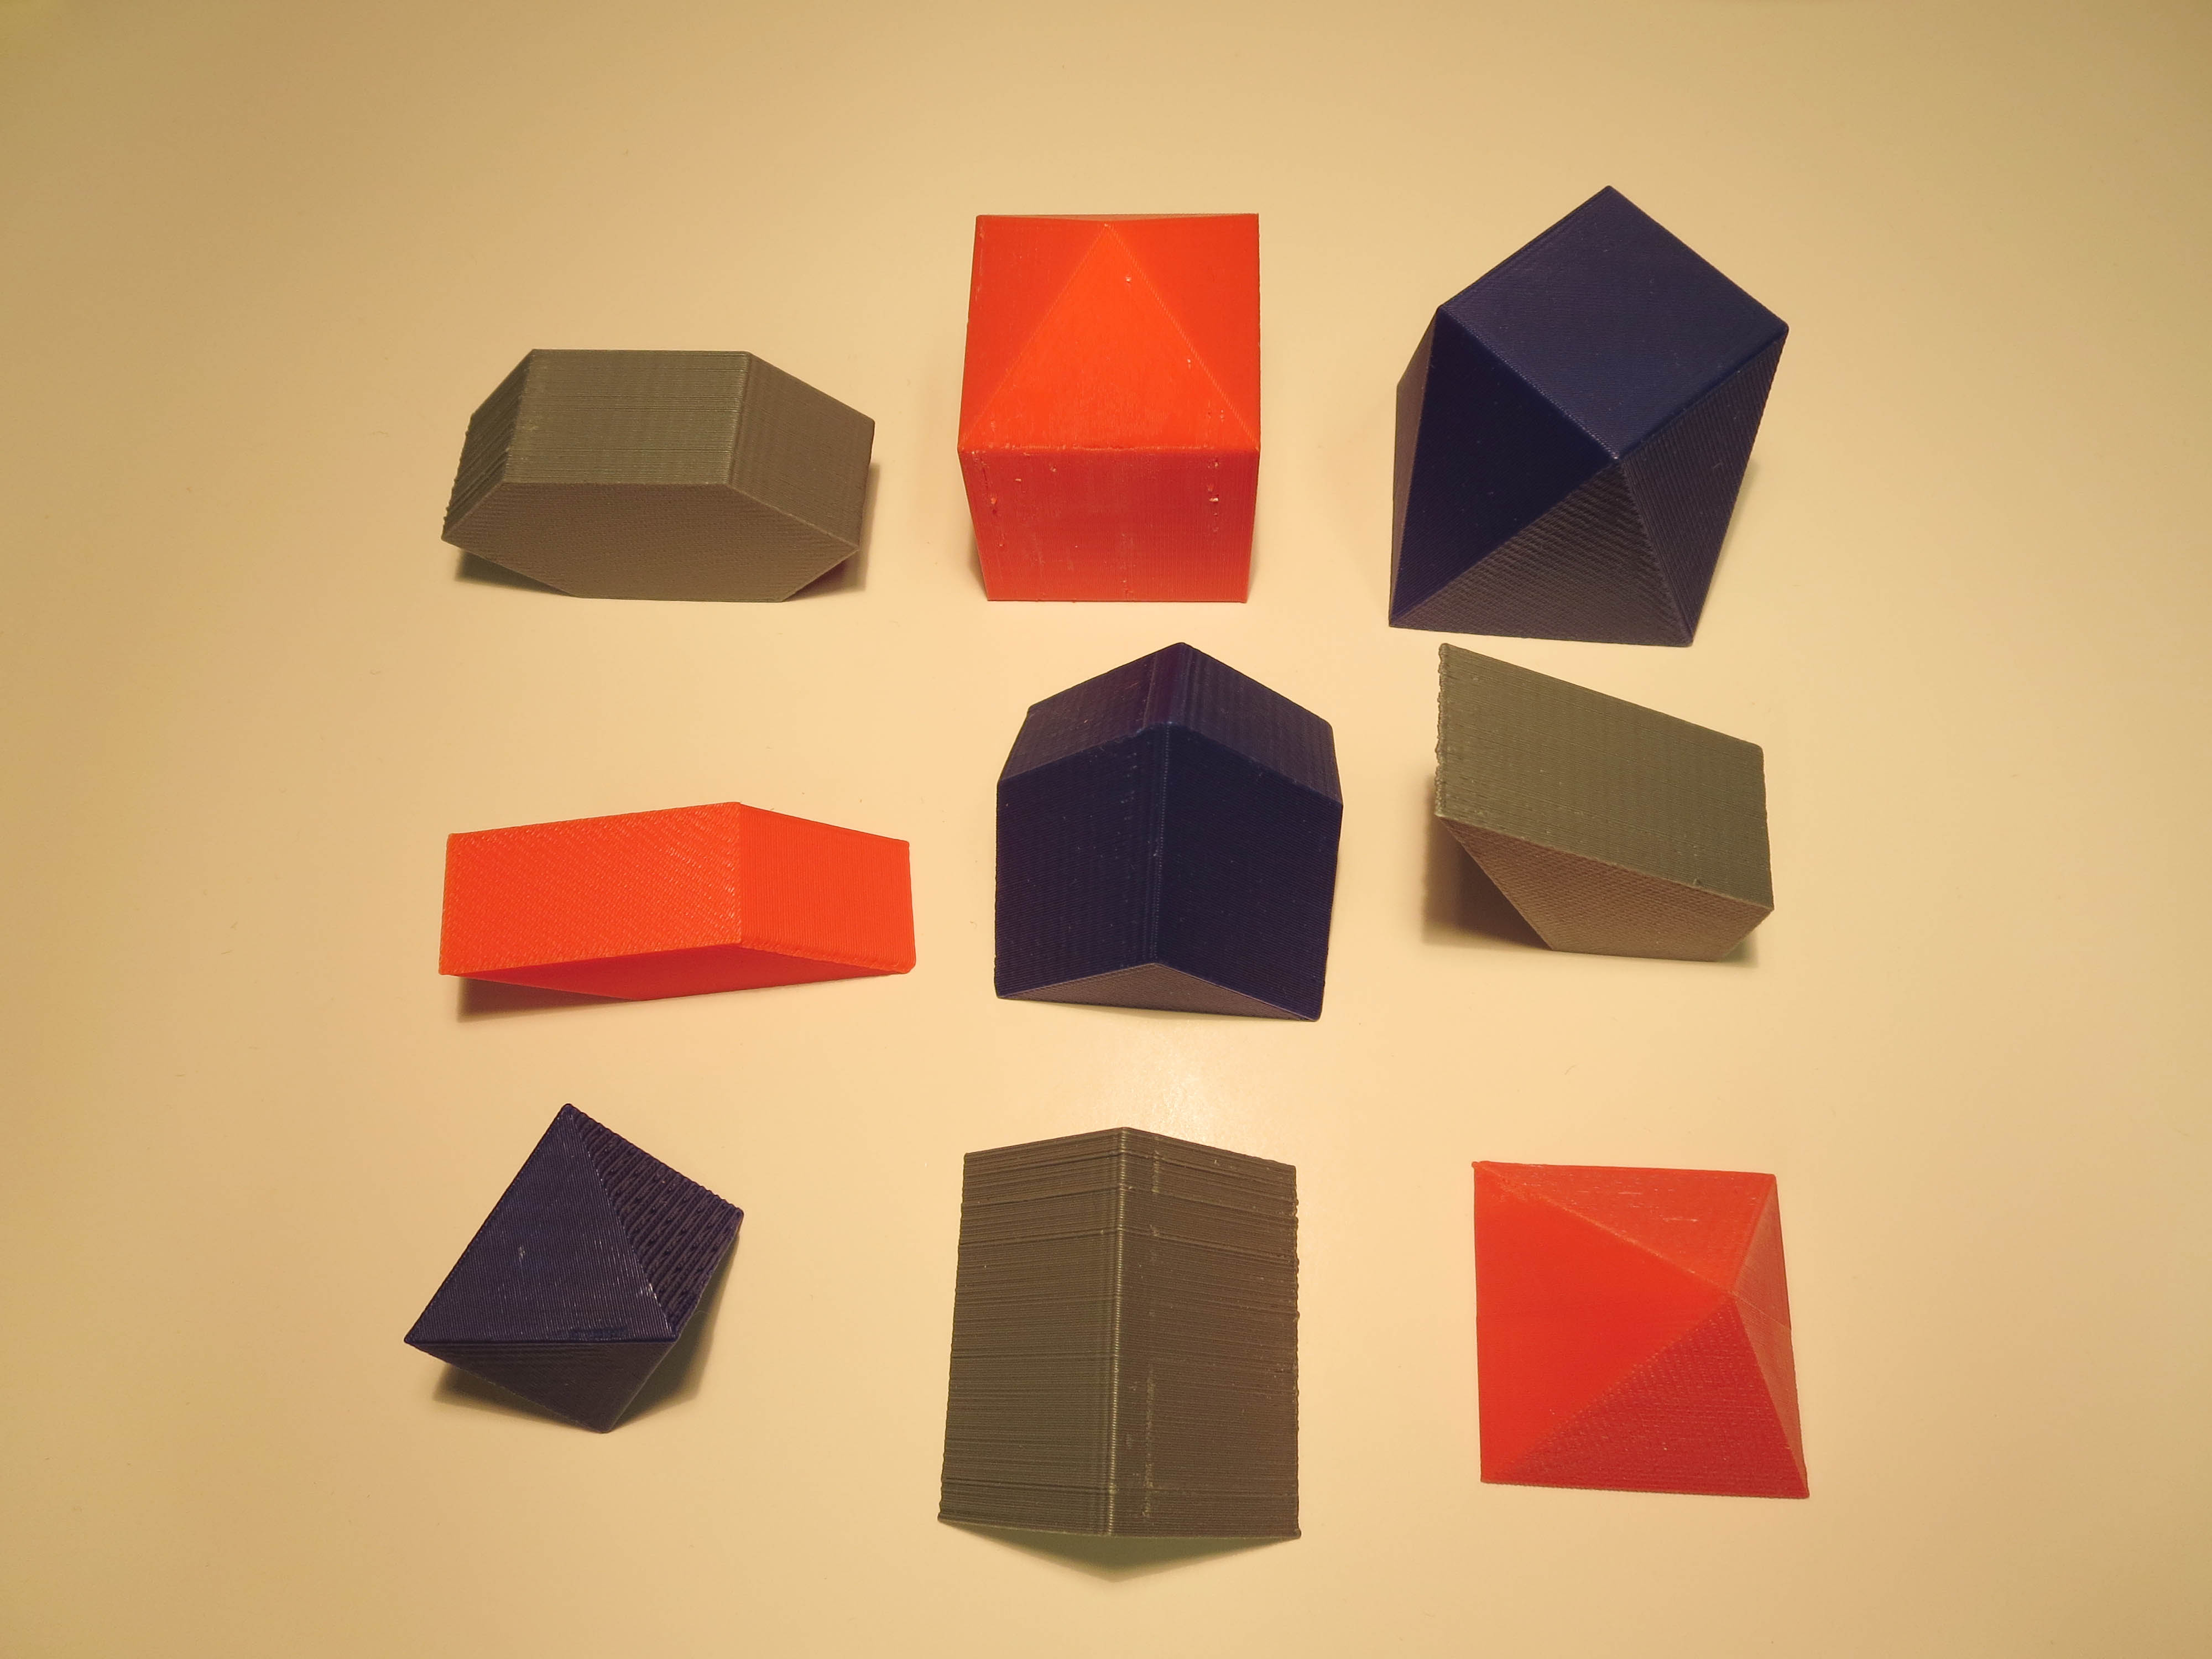
\includegraphics[width=.5\linewidth]{images/hulls}
\end{center}
\caption{A collection of 3D printed shapes modeled using the convex hull mode in
the software with the devices mentioned earlier in this chapter.}
\label{fig:hulls}
\end{figure}



\subsubsection{Paths: Creating Linear Forms and Knots} 
In the convex hull examples in the previous paragraphs, we have not made use of
the fact that the software samples selected points in real time: thus, when a
user adds or subtracts a point in space, that change is registered immediately
in the desktop software. What this means is that the user can exploit not only
the overall set of selected points, but can also make use of the \emph{order} in
which those points are selected. A sequence of selected points need not
represent only vertices of a solid; it can also represent a path over time in 3D
space. Figure \ref{fig:paths} shows several sample projects based on this idea.
Here, the software has been employed to read points as successive positions of
various routes through 3-space. The resulting paths have been printed out on a
3D printer.

In some cases, the path is closed, finishing at the same location where it
started; the path printed out at center in red in Figure \ref{fig:paths} is in
fact a well-known mathematical form, a trefoil knot. (It may be worth mentioning
here that such a knotted form would be rather tricky to create in standard 3D
modeling software, but the form can be created ``by hand'' with our devices,
selecting light positions in space along the path of the knot.)

\begin{figure}[!ht]
\begin{center}
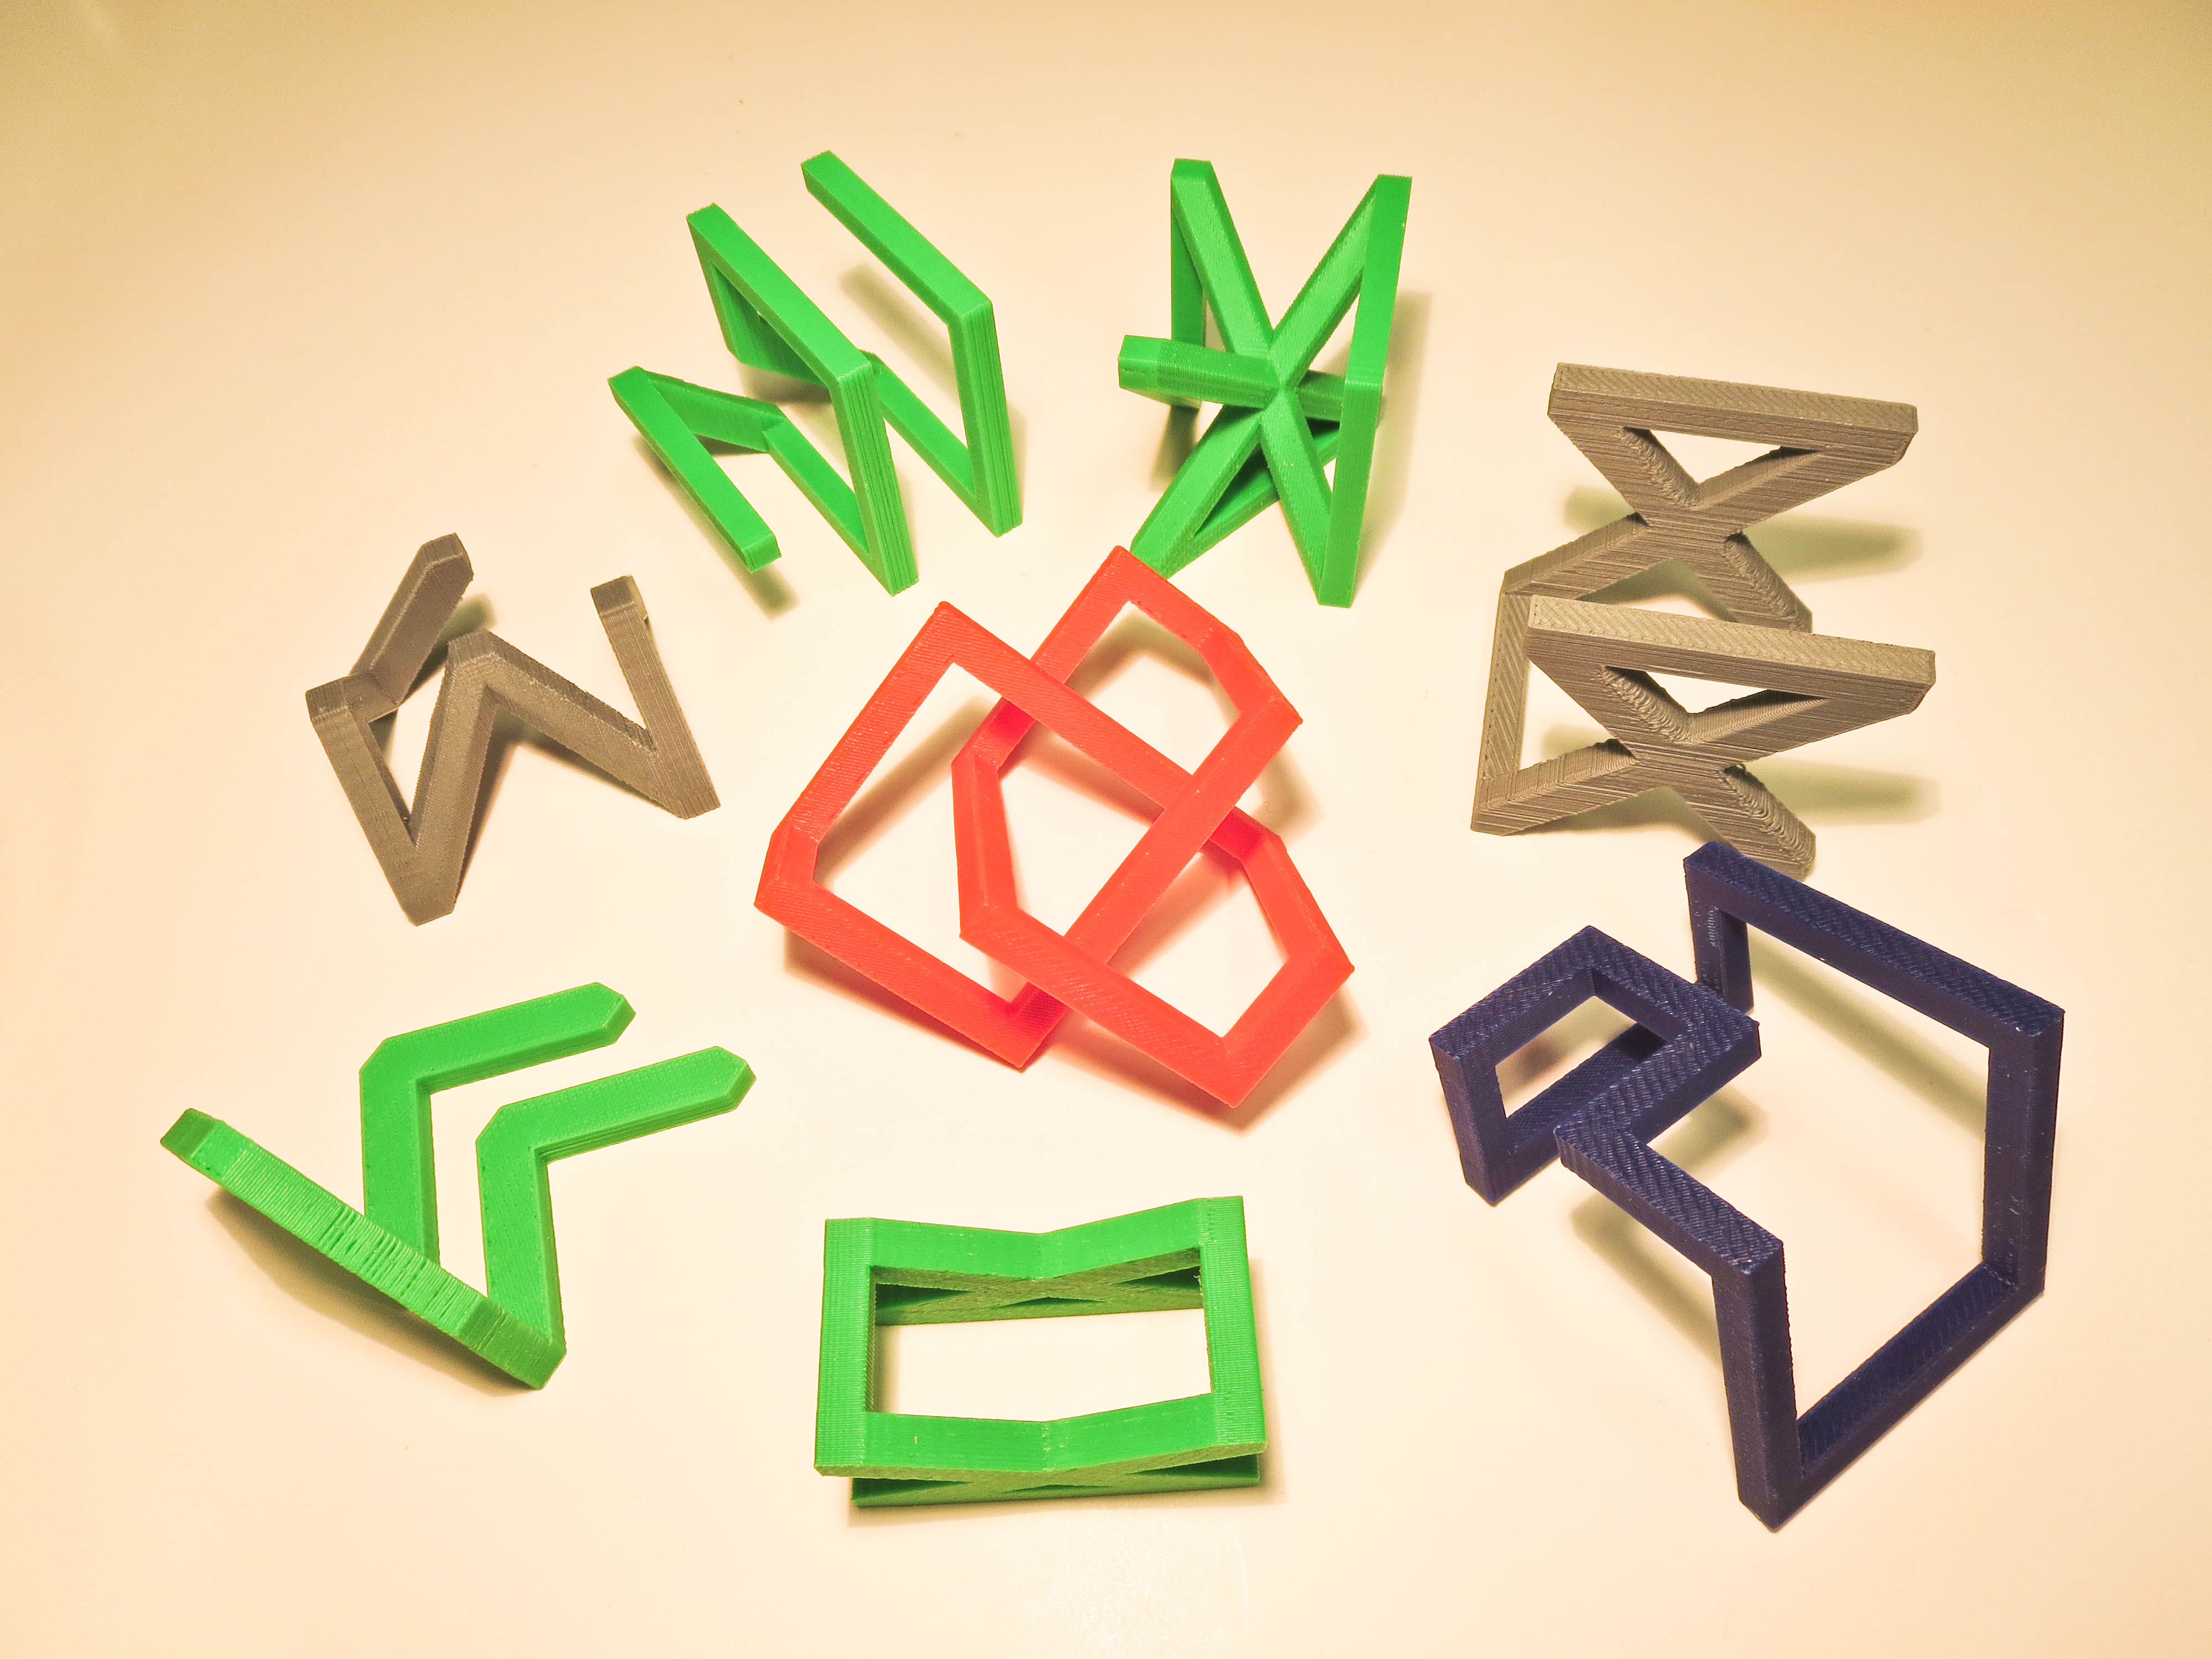
\includegraphics[width=.5\linewidth]{images/paths}
\end{center}
\caption{A collection of paths modeled on our devices using the path mode in
the software, exported from the software and 3D printed in our lab. The red
shape in the middle may be recognizable as a traditional trefoil knot.}
\label{fig:paths}
\end{figure} 

To briefly explain the workings of this mode, then: each point on the device is
stored, in order, in an array. Once the second point of the path is added (one
point a path does not make), each point is then ``exploded'' into a cube,
centered on the point. The size of each cube is controlled by the ``path width''
slider, so the single original point generates 8 points, offset by the current
value of the path width slider (e.g., Point p1 = new Point(x + offset, y +
offset, z + offset);). The algorithm then takes the cube of points associated
with each pair of connected points (e.g., points 0 and 1, 1 and 2, 2 and 3,
etc.) and runs the convex hull algorithm discussed earlier, generating a sort of
rectangular prism between the two cubes. By connecting each new point to the
previous one, a trail of rectangular prisms is generated between the points
specified, in the order in which the user placed them. Figure
\ref{fig:trefoilPath} shows a trefoil knot created with the path mode. By
highlighting the strokes in red, one can see that each point is in fact
surrounded by a cube, while each cube is connected to its neighbors by
rectangular prisms.

\begin{figure}[!ht]
\begin{center}
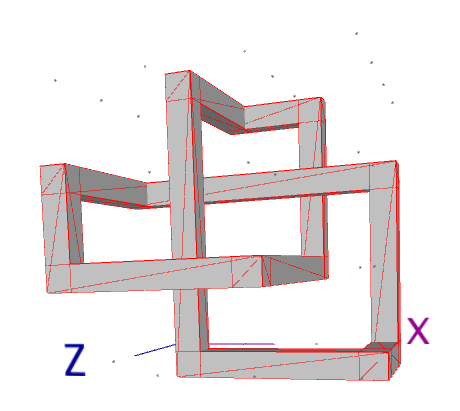
\includegraphics[width=.5\linewidth]{images/trefoilPath}
\end{center}
\caption{A trefoil knot, as modeled on the UCube version of the software.
The outlines (strokes) of the knot have been highlighted in red to show the
manner in which the software constructs the path; points are expanded into
cubes, and adjacent pairs of cubes and then connected with rectangular prisms
(the convex hull of two separated cubes).}
\label{fig:trefoilPath}
\end{figure}

The utility in creating a mode like path is fairly self-explanatory; it allows
for a vast number of shapes to be modeled, of a wholly different class of
objects as the traditional polyhedral style of the convex hull output. As we
will discuss in greater detail later, this method was popular with children who
used it; in some ways it is akin to writing or drawing, albeit in 3D, where once
you have a pen on paper, a line will follow wherever you move your hand. The
path mode allows for the creation (or close approximation) of most English
letters and numbers, common symbols (like stars), and 3D outlines of normally 2D
geometric shapes, like triangles and rectangles.


\subsubsection{Points as ``Blocks'': Creating Non-Convex Polyhedral Forms} 
Aside from the convex hull and path operations noted above, the device allows
for multiple different semantics for spatial locations. For example, in the path
mode previously mentioned, if we choose to construct paths with an edge-length
of one ``interval unit'' of the given device - achieved by putting the software
in path mode and setting the ``path width'' slider to one-half of the distance
between points - each cube created will fit perfectly next to its neighbors,
turning each point into a sort of ``block'' . In this way, selecting (say) four
successive light locations along the length of one tower, then, one could
specify a rectangular prism. Likewise, by selecting three point locations in an
``L'' form, one could specify the non-convex polyhedral form seen at the far
left of Figure \ref{fig:soma} below.
 
\begin{figure}[ht] \begin{center}$
\begin{array}{cc}
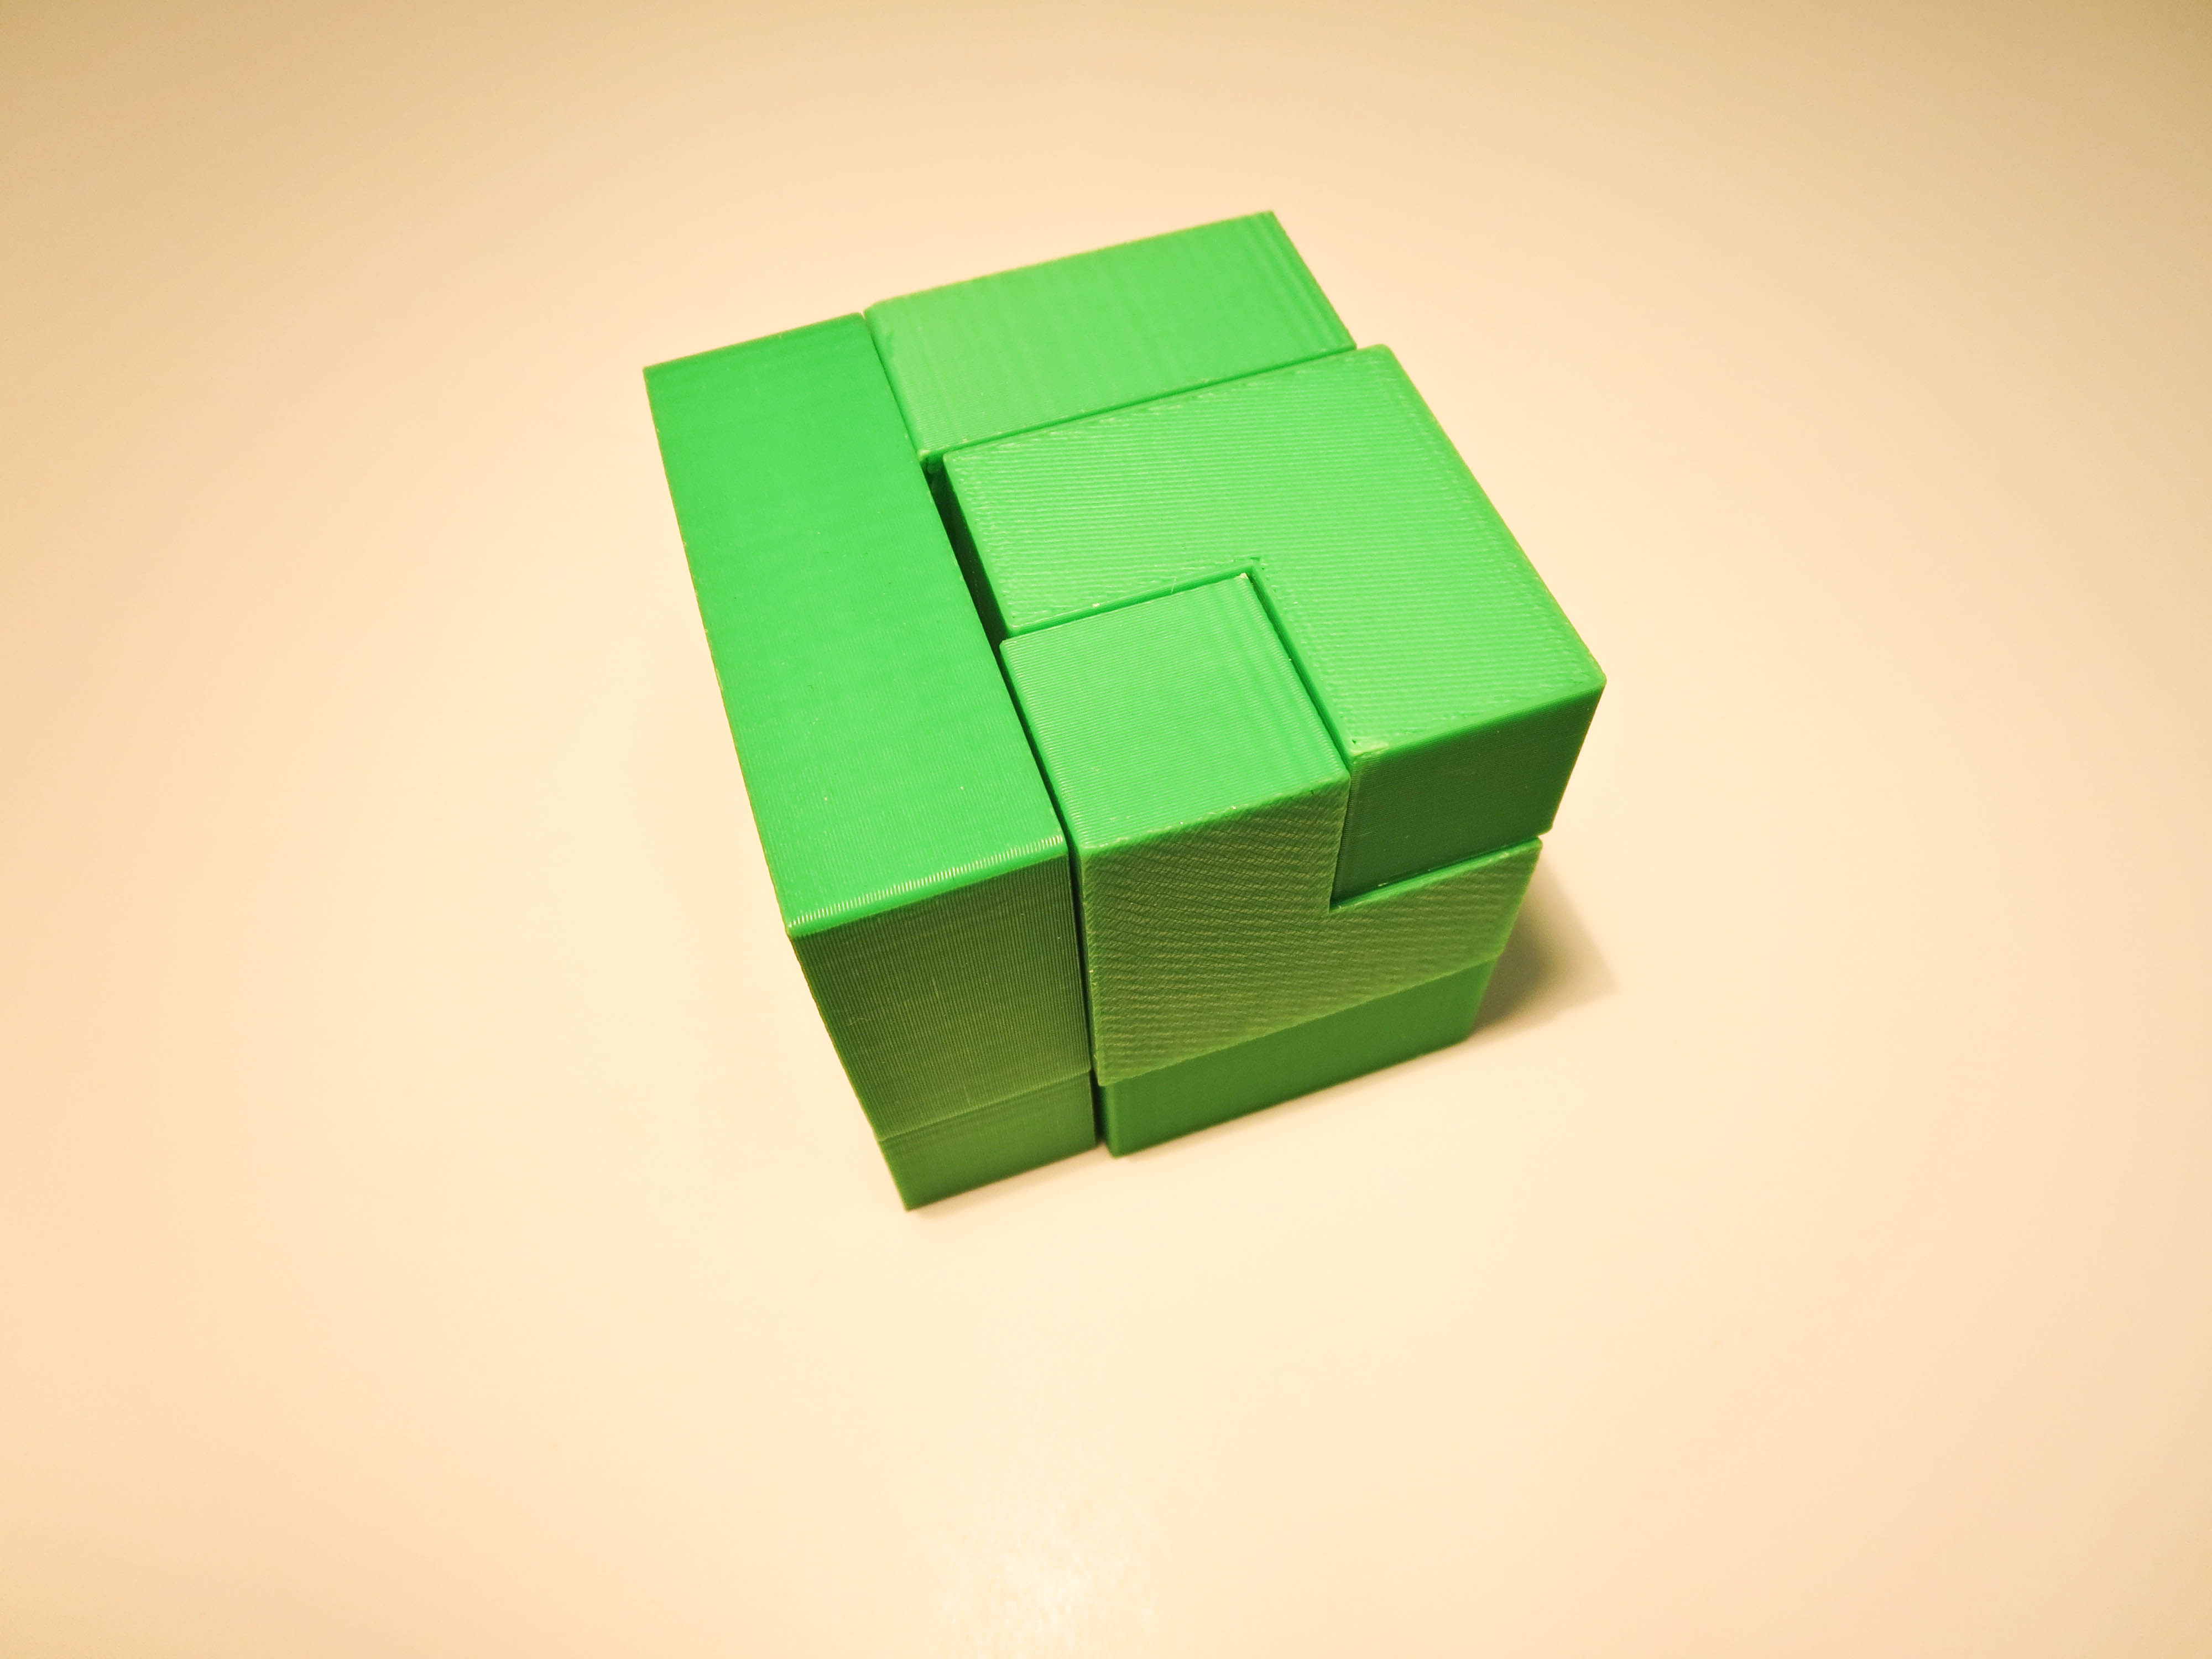
\includegraphics[width=.46\linewidth]{images/somaCube} &
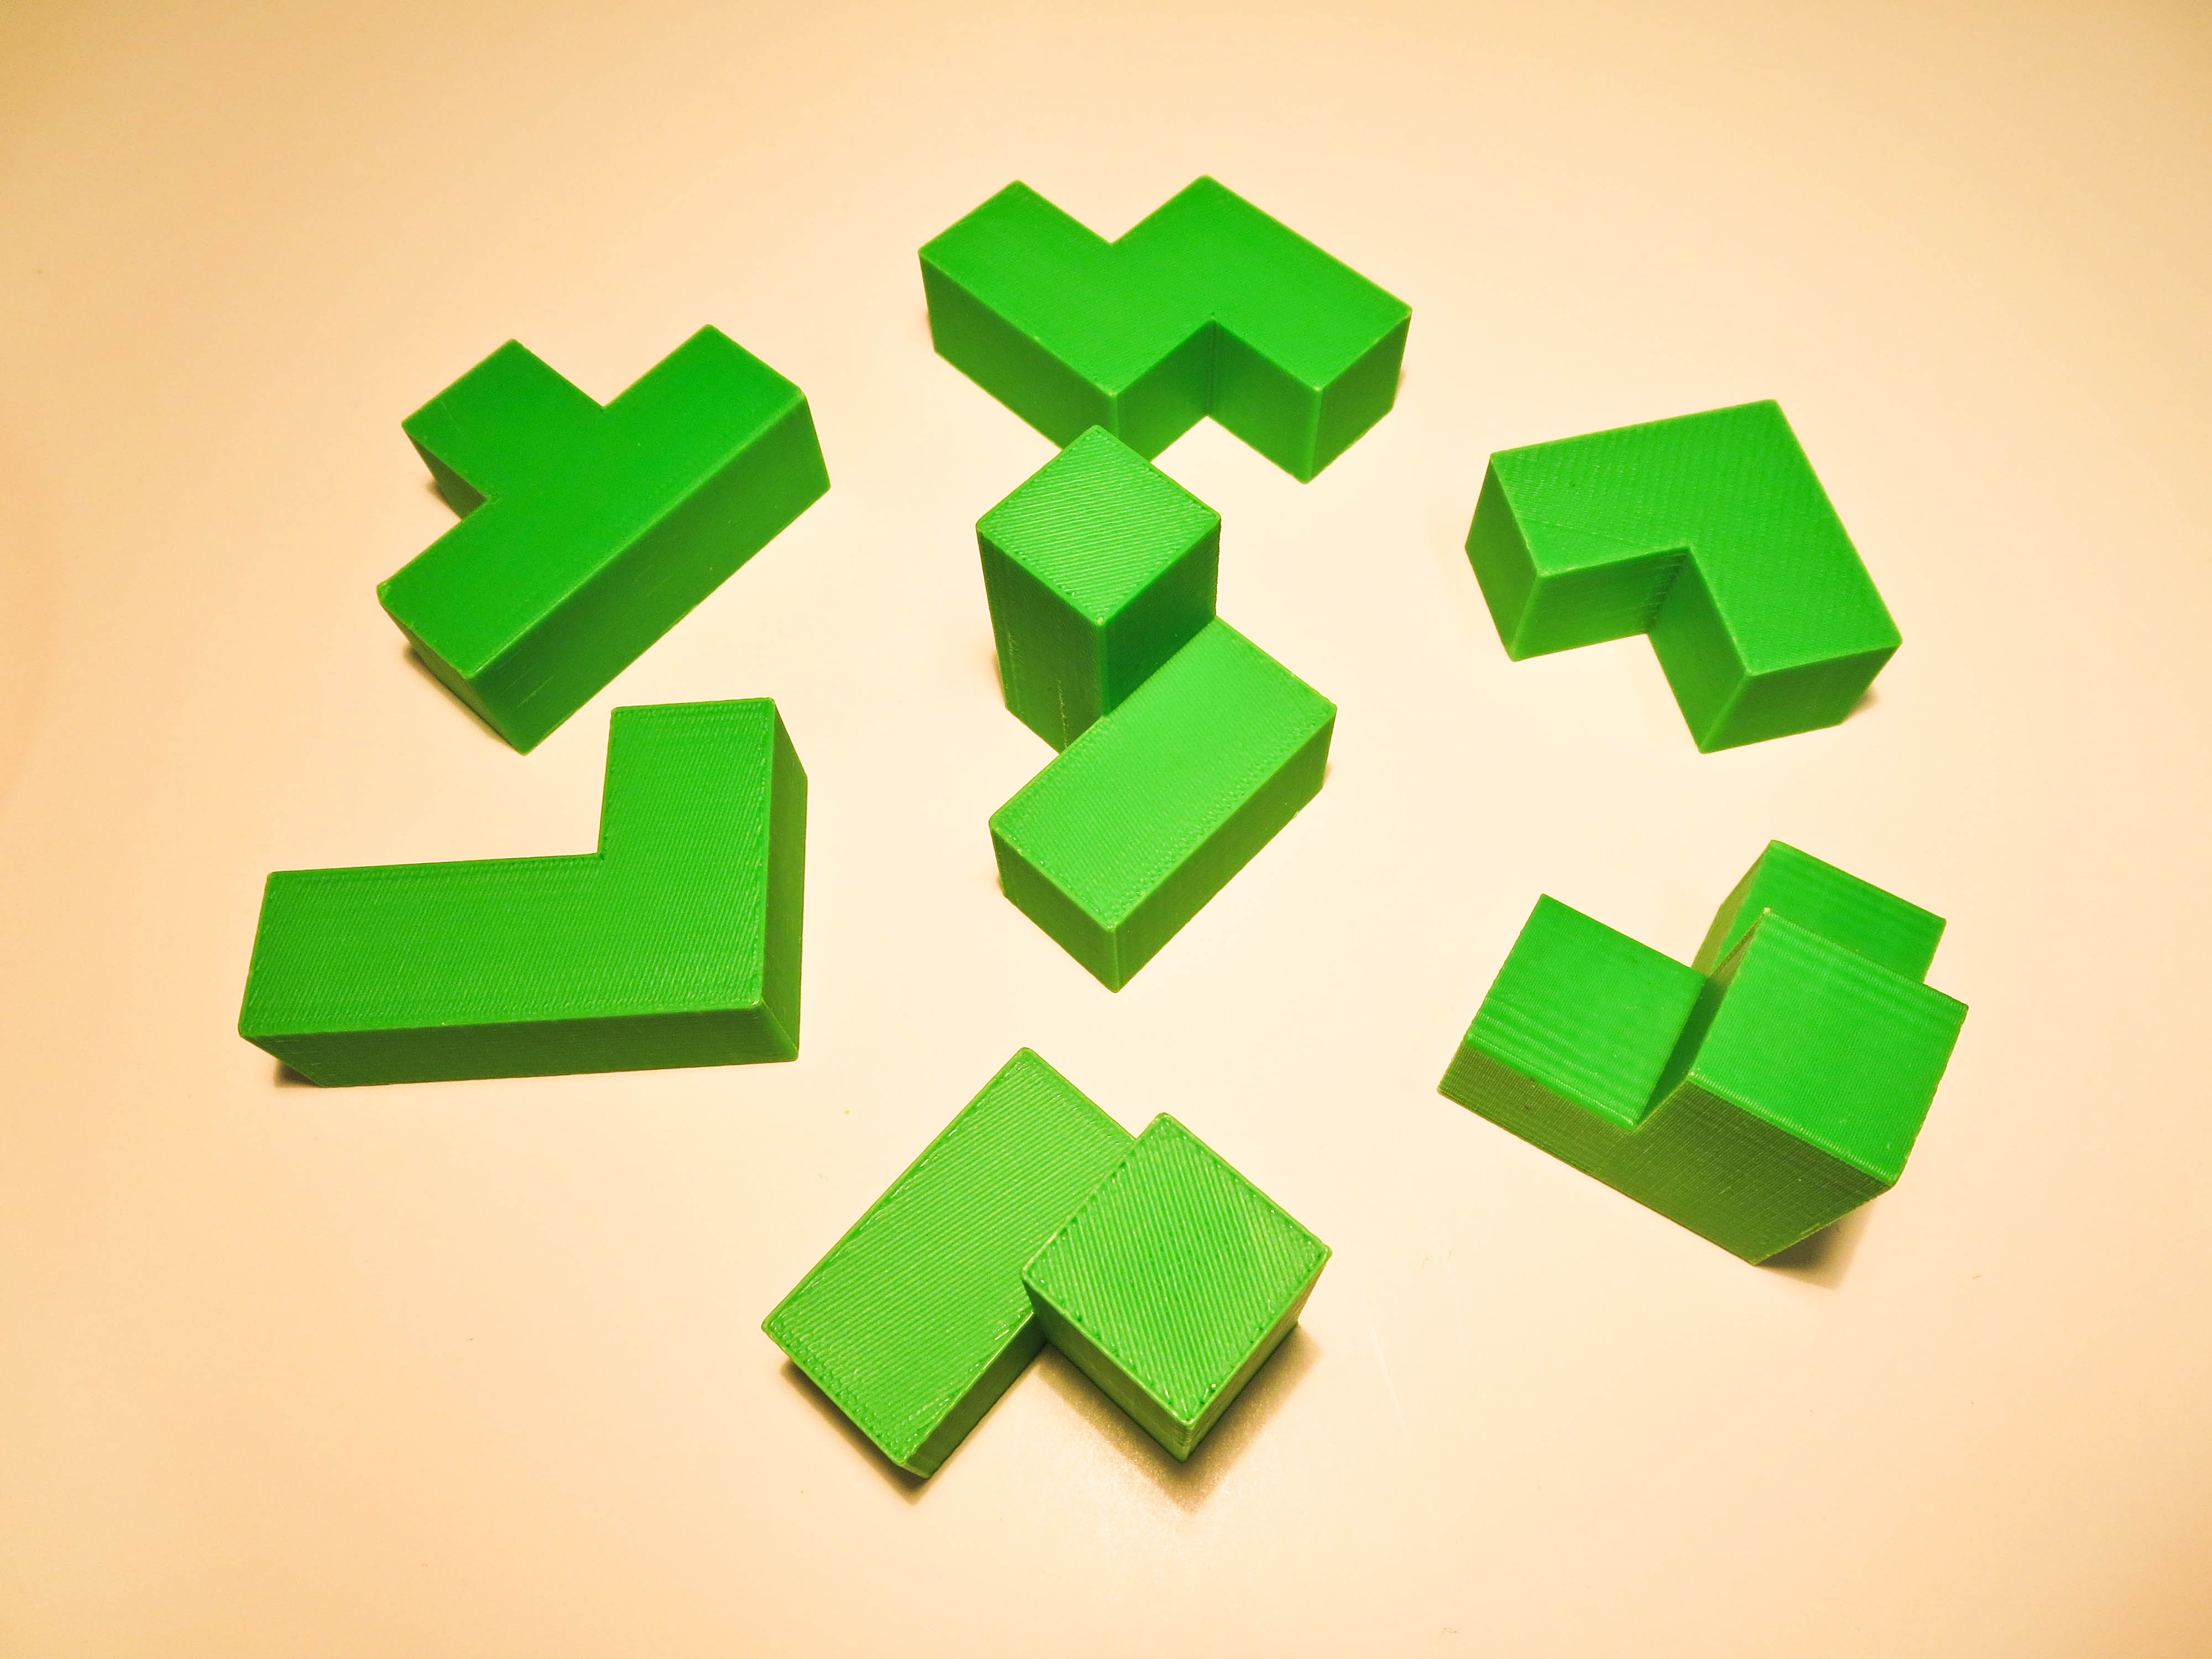
\includegraphics[width=.46\linewidth]{images/somaPieces}
\end{array}$
\end{center}
\caption{A set of non-convex polyhedral forms modeled on the UCube, which
constitute the well-known ``Soma Cube'' puzzle, shown assembled on the left
with the individual shapes laid out on the right.}
\label{fig:soma}
\end{figure}

This technique for using the path mode has some interesting advantages in terms
of the physical properties of the paths produced in this manner. For those
readers interested in recreational mathematics, the shapes shown in Figure
\ref{fig:soma} will be recognizable as the component pieces of the ``Soma''
puzzle; these pieces can be arranged together to form a larger cube (also shown
in \ref{fig:soma}). The software could be employed with any of the devices in
similar fashion to produce many such dissection-type puzzles, building blocks,
or other for other domains where interlocking, block-like shapes may be useful:
architectural mockups, model train environments, real-life Tetris, and a myriad
more.

\subsubsection{Point Clouds: Creating Minimal Spanning Trees}
Instead of interpreting points as vertices of a solid (as in the convex hull
examples) or as the successive stations of a temporal path (as in the ``path''
examples above), we could in fact simply treat our set of points as just what
they are � namely, a set of points. Starting with this interpretation, we might
produce a form such as a minimal spanning tree of the set of points (a set of
edges of minimal total length connecting all the points). Figure \ref{fig:trees}
shows several examples of forms created this way; one immediately grasps the
variance and complexity that this mode is capable of. The yellow ``jack'' in the
middle of \ref{fig:trees} is the product of nine points, eight of which form the
equidistant vertices of a cube (or what would form a cube if the software were
in convex hull mode), with the last point perfectly centered in the middle,
effectively ``bending'' the rest of the graph segments in to meet it.

\begin{figure}[!ht]
\begin{center}
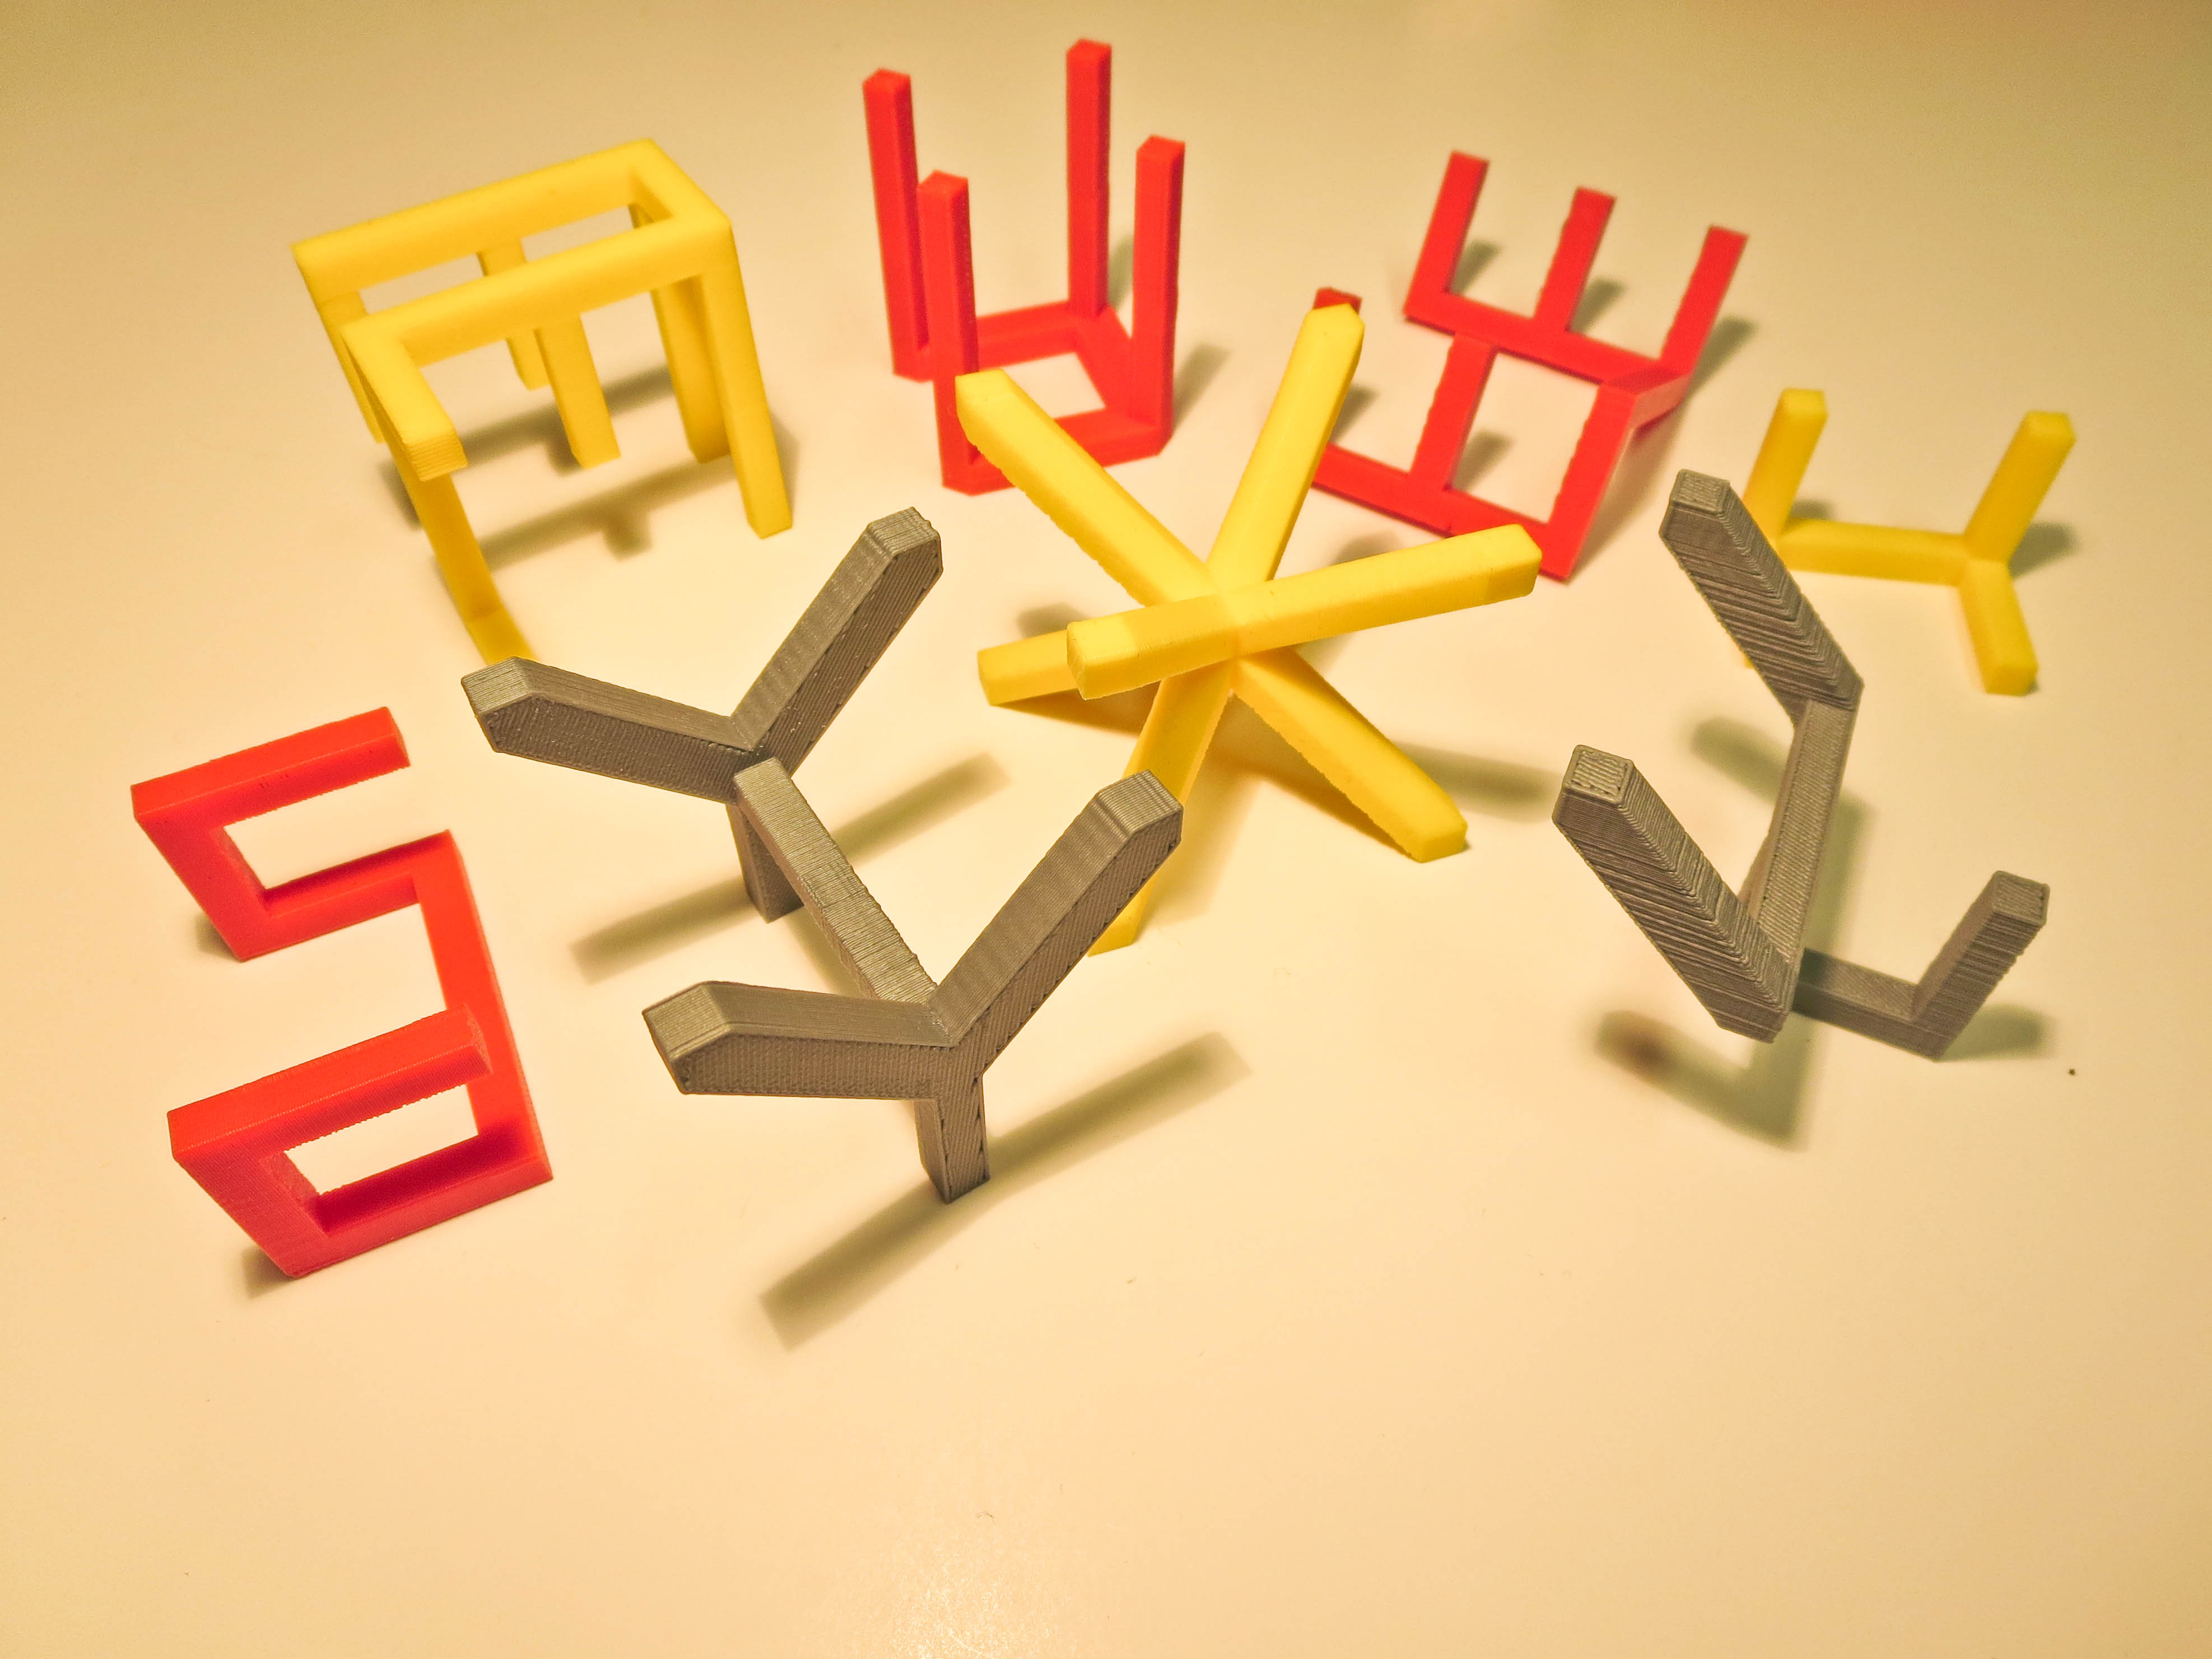
\includegraphics[width=.5\linewidth]{images/trees}
\end{center}
\caption{Several examples of models produced using the minimal spanning tree
mode in our software, exported, and printed out on a 3D printer.}
\label{fig:trees}
\end{figure}

As with the convex hull, the minimum spanning tree is a well-defined,
extensively studied algorithm in computer science and mathematics. Given a set
of points on a graph, the minimal spanning tree will be a solution (possibly
more than one) that connects each point on the graph, without cycles (returning
to a point already in the tree), and with the minimal possible value of some
``cost'' variable, often defined as the sum of ``weights'' of the connected
edges in the tree. One may think of the minimal spanning tree like constructing
a subway system, where all the stations need to connect and the length of
track should be minimized to keep construction costs as low as possible.

The first algorithm for finding the minimum spanning tree was derived by a Czech
scientist, Otakar Bor\r{u}vka in the late 1920's\cite{boruuvka1926jistem}, for
the purpose of planning electric distribution networks. There are two popular
algorithms used today, Prim's and Kruskal's both of which are considered
``greedy'' (by iteratively choosing the locally optimal edge to determine the
spanning tree) and run in polynomial time.
Our software uses an implementation of Kruskal's algorithm, whereby Euclidean
distance between two points on the graph is used as that connecting edge's
weight. Kruskal's algorithm, first described in 1956\cite{kruskal1956shortest},
starts by taking a set of each vertex (thought of as separate trees) and a set
of all the possible edges in the graph (with their corresponding weights), then
iteratively removes the edge with the lowest weight from the set of edges and
adds it to the set of vertices, connecting two of these trees into one, until
there is only one tree left from the original set of vertices (or we run out of
edges to pull from). If there is only one tree left in the vertex set, then that
tree represents the minimal spanning tree. It is, of course, possible to have
more than one minimal spanning tree for a given graph however.

In our software, we run Kruskal's algorithm whenever a point is added or removed
in ``tree'' mode. The set of points is sent as inputs, the edges and edge
distances are calculated, the algorithm is run, and returns a list of connected
edges, the set of which is the minimal spanning tree. This list of edges is
treated in much the same way as the points in ``path'' mode: each edge has two
point coordinates, both of which are ``exploded'' into cubes centered on the
point, and then the set of two cubes (16 points) are sent to the convex hull
algorithm, creating a 3D rectangular prism between the two cubes.

Including the minimal spanning tree mode is an interesting departure from the
convex hull and path modes; it is not easily explained to the novice designer,
nor does it have the sort of intuitive relationship to the set of active lights
as the other modes do. The addition or subtraction of a single point can
radically alter the resultant spanning tree in (sometimes) unexpected ways - not
so with the convex hull or path modes. However, it is this lack of immediate
understanding and the element of unexpectedness that makes this mode a good fit
for the kind of devices we make. The real-time adjustments of the software in
combination with the exploratory nature of the devices makes the tree mode
highly engaging (in our observations, explained in full later on). The ability
to quickly add or remove points from the graph is a feature unique to our
devices and allows for a quick way to ``check and see'' different combinations
of points and strategies, while being able to look between the device and the
software and start to draw some conclusions about how their actions affect the
shapes being displayed.

\subsection{Other Software Functionality}

The software modeling modes mentioned in the last section set the stage for the
types of figures that can be constructed with our devices, the software has
additional features that are crucial to the overall purpose of the system. This
section will go over the operation and methodology of the most important of
those: the software's ``Edit'' mode and the ``Export'' feature, allowing figures
to be saved in a 3D-printer friendly format.

\subsubsection{Edit Mode}

In order to (partially) address the ``inflexibility'' inherent in having points
and thus shapes confined to the integer lattice, we developed a way in the
software to ``edit'' the points by putting the software into a special mode that
freezes the serial input from the connected device and allows the user to
click-and-drag points off their ``hardware defined'' locations. The edit mode
affects all three of the modeling modes mentioned above, so the user can how the
edits they make change each modeling algorithm. We also provide a ``reset''
button as a way to ``snap'' back to the original grid of points.

The mode works by combining several pieces of functionality that work together
to keep track of the cursor position (to detect if it is hovering over a point)
and its click-state, track the relative position of the point as it is being
moved, and relay that position information to the data structures responsible
for the different modeling modes - all in real time.

\begin{figure}[!ht] \begin{center}$
\begin{array}{cc}
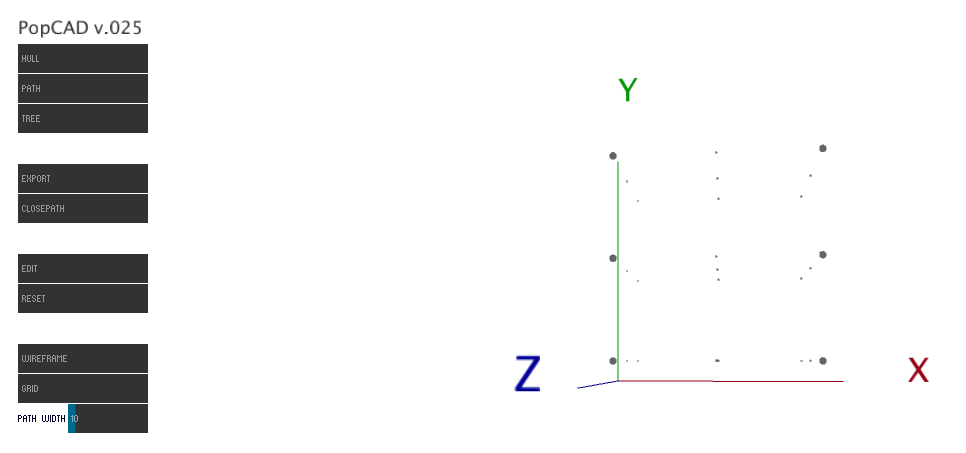
\includegraphics[width=.44\linewidth, height=1.6in]{images/edit1} &
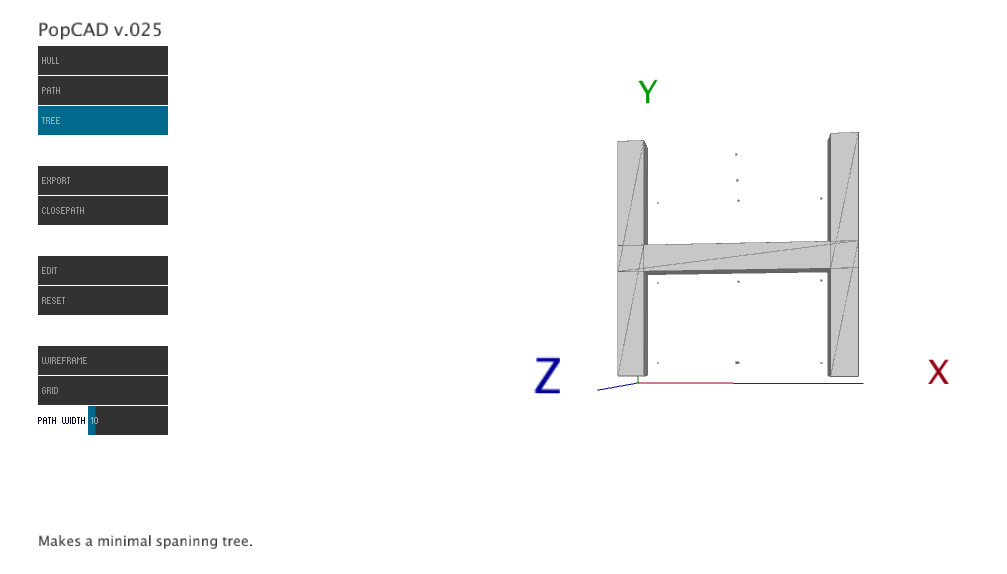
\includegraphics[width=.44\linewidth, height=1.6in]{images/edit2} \\
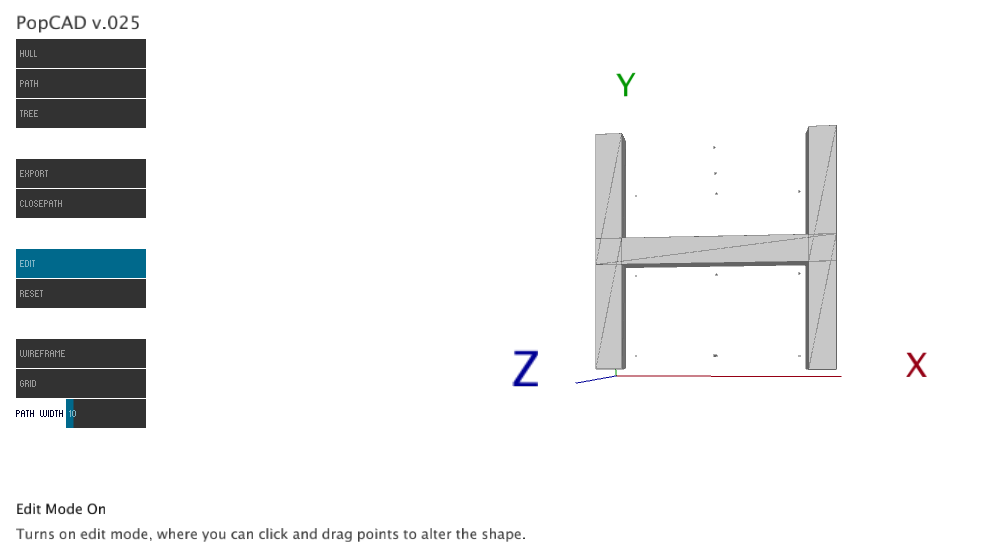
\includegraphics[width=.44\linewidth, height=1.6in]{images/edit3} &
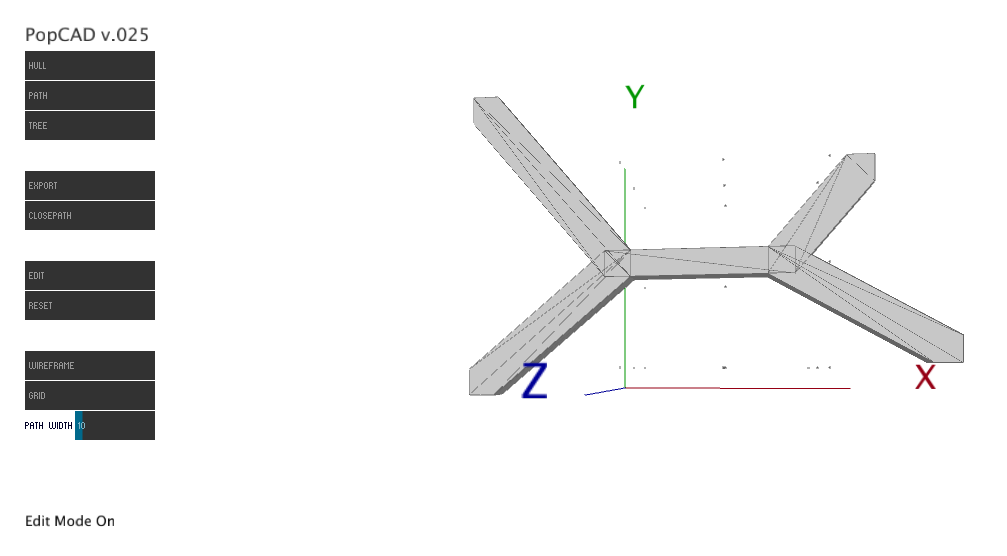
\includegraphics[width=.44\linewidth, height=1.6in]{images/edit4}
\end{array}$
\end{center}
\caption{A four step sequence showing the operation of the edit mode: (upper
left) six unaltered points; (upper right) the points form an ``H'' shape
with tree mode selected; (lower left) the selection of edit mode; (lower
right) the edited shape, with the corners of the original shape extended
outward.}
\label{fig:editMode}
\end{figure}

Figure \ref{fig:editMode} shows a four-step sequence of screen shots using the
edit mode to alter a shape: (upper left) six points have been lighted on the
PopCAD and are reflected as simple points in the software; (upper right) the
user has selected ``tree'' mode, taking the minimal spanning tree of the six
points, forming a sort of ``H'' pattern; (lower left) the user selects the
``edit mode'' button, freezing the serial input and initiating the
click-and-drag editing ability; (lower right) the user has dragged each of the
four ``corner'' points outward, altering the original shape into something new,
impossible to model using only the ``raw'' points available on the device.

\subsubsection{Stereolithography Export}

One of the most important functions of the software is to make a user's
creations into easily 3D-printable shapes. Many complex 3D software programs
allow for export into sterolithography format (.STL), which is the common input
format for 3D printer software programs, however, these programs rarely check to
ensure that the produced file will actually be printable; many ``model-able''
shapes will cause errors in 3D printer software - lines, 2D shapes, shapes
within shapes, shapes with gaps between faces - and on and on. Our software also
exports into .STL format, but takes great pains to ensure that any exported file
will print without error.

The export function in our software deals with models formed from all three
modes simply by keeping track of the active mode and choosing the correct export
method accordingly. The export process is similar for each type of shape: since
each shape is actually constructed of one or more convex hulls, the array of 3D
vectors describing (in order) each triangulated face of the hull (or hulls) is
added to a triangle mesh, which takes in all the faces, flips the Y axis
values for each coordinate (because in the Processing environment, (0,0) is in
the upper left), flips the vertex order, which corrects problems with sliceform
errors (in 3D printing software) resulting from the face normal vectors facing
the wrong way, then adds all the faces to an .STL object, which outputs a series
of triangles in an .STL file the describes the object.

\begin{figure}[!ht]
\begin{center}
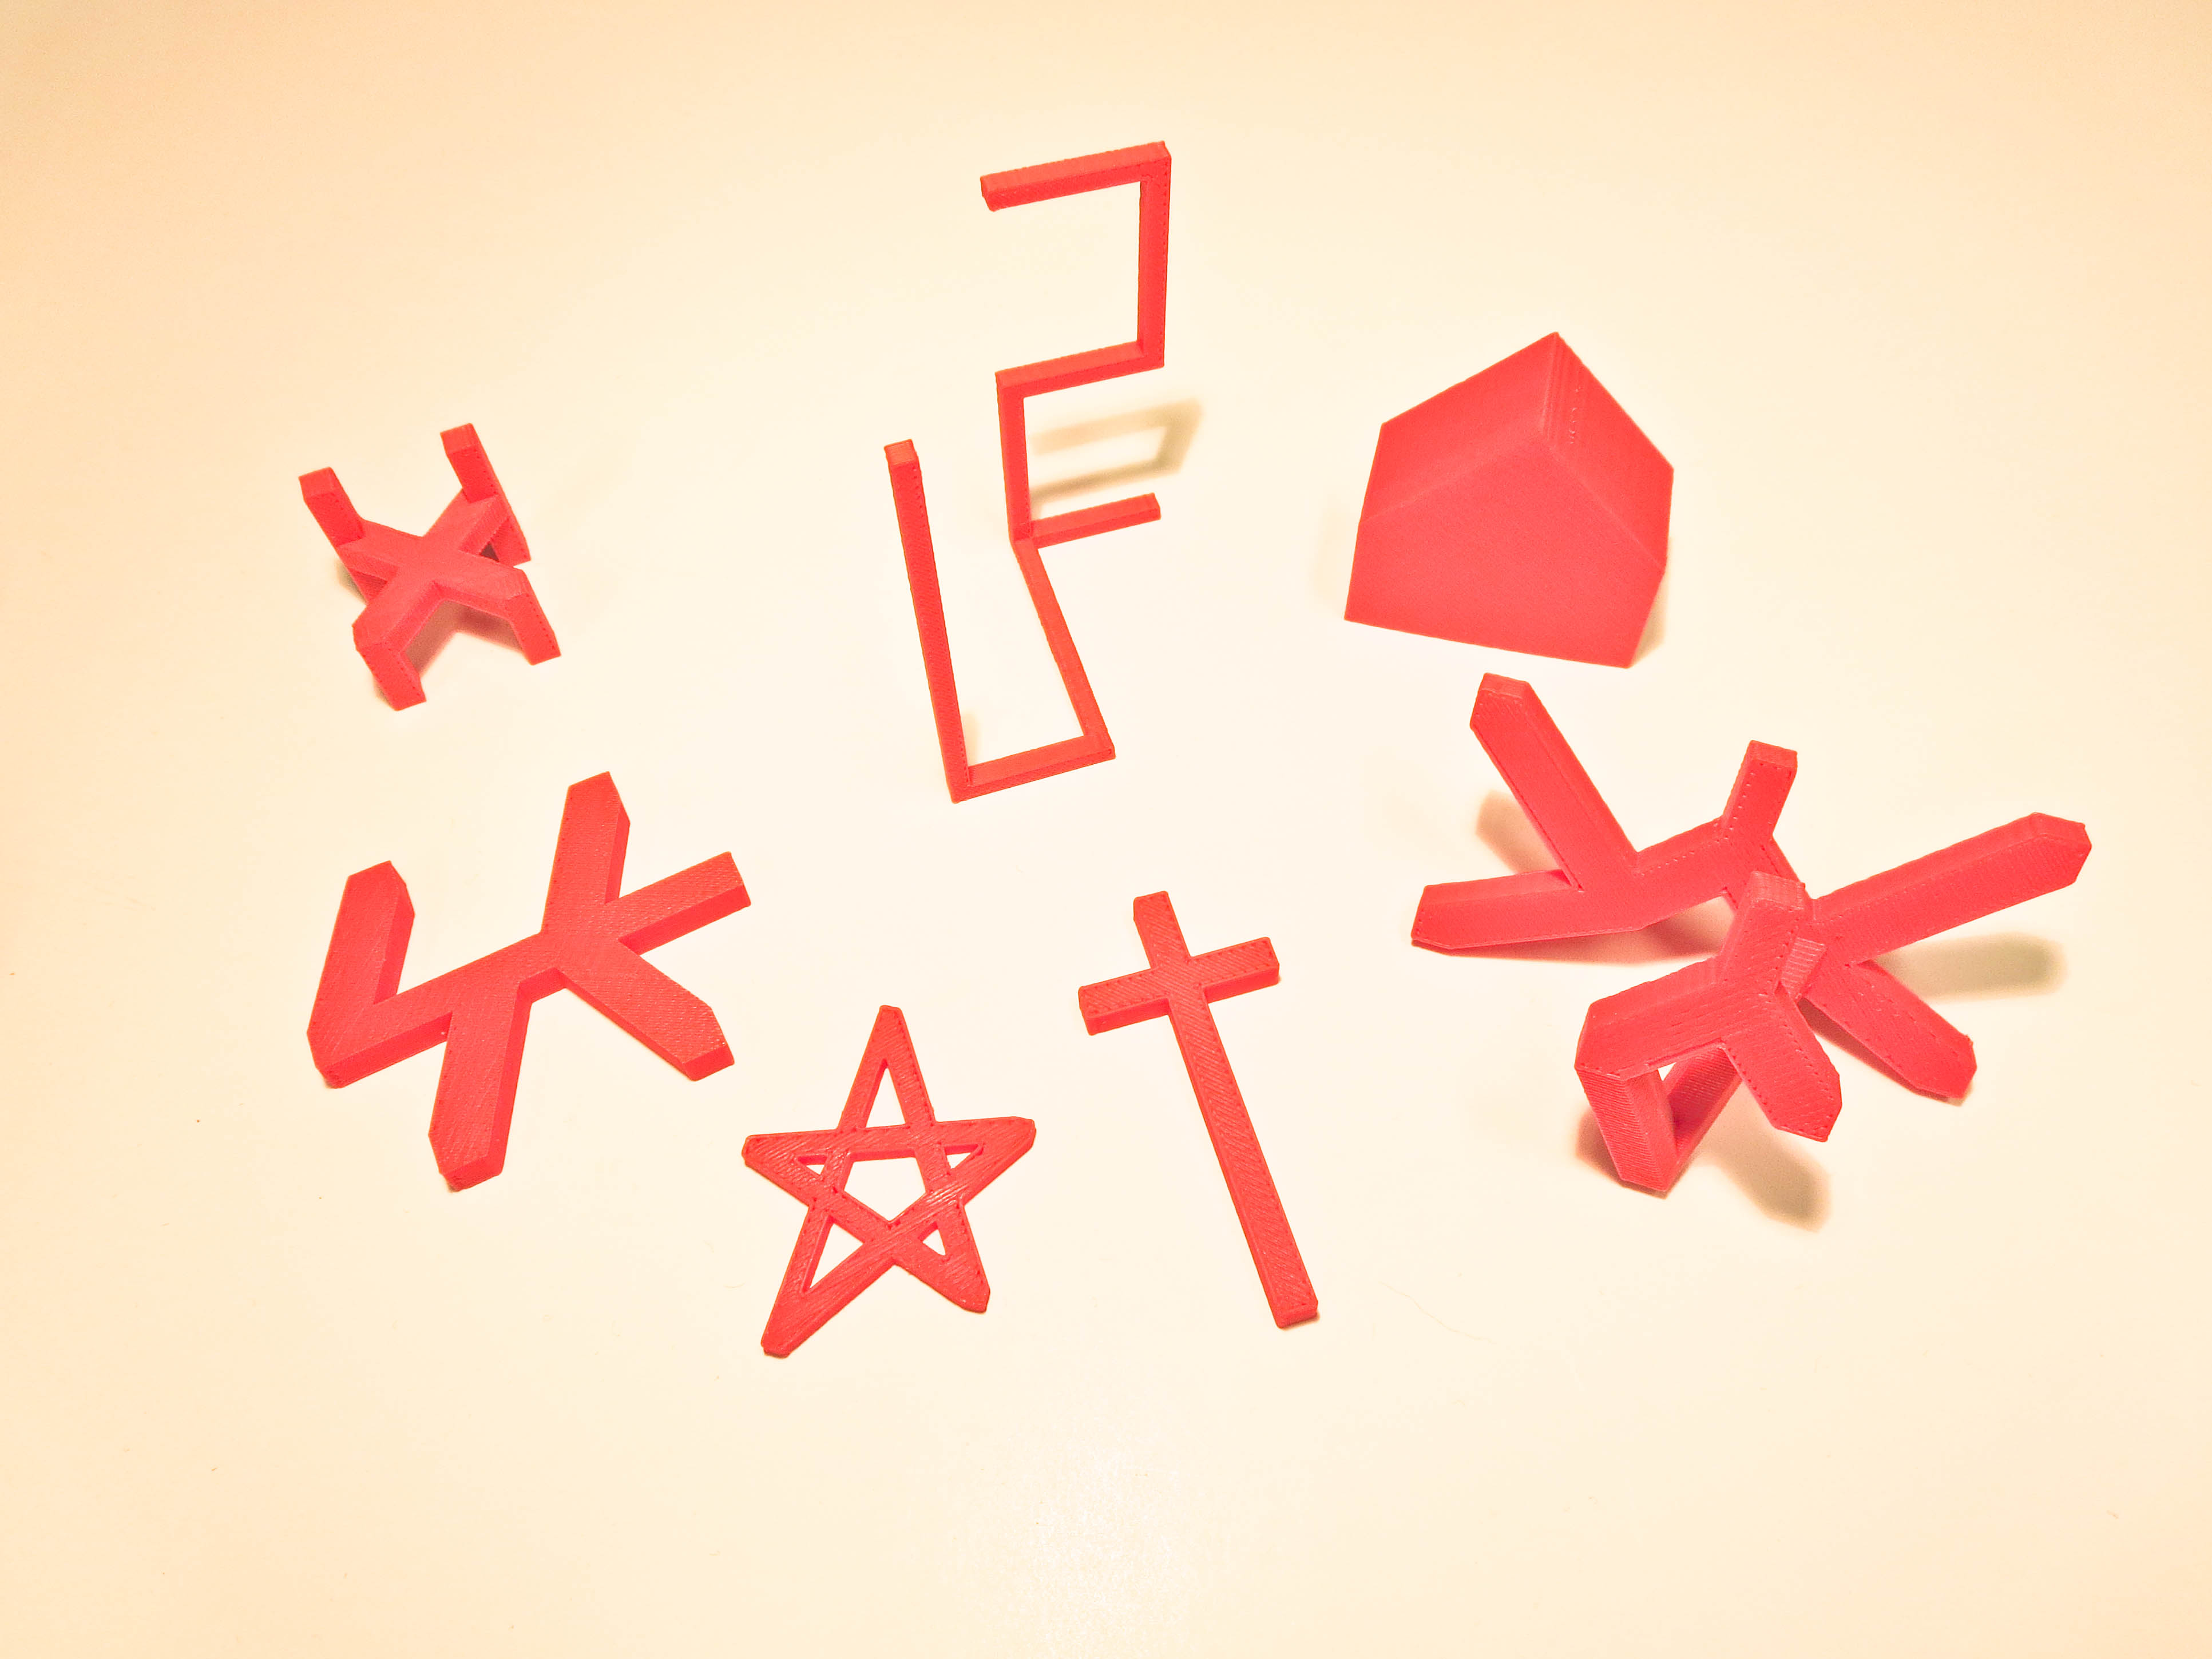
\includegraphics[width=.5\linewidth]{images/userShapes1}
\end{center}
\caption{Several of the shapes modeled on the PopCAD and SnapCAD devices by
novices designers (most of them without any previous 3D modeling expertise)
from one of the user studies we performed.}
\label{fig:userShapes1}
\end{figure}

Creating a ``novice-proof'' stereolithography export (all of the above
computation happens with one click, even the file naming) is crucial to the
raison d'\^{e}tre of our work - to democratize the process of designing
meaningful, personalized objects for 3D printing by novice designers. See Figure
\ref{fig:userShapes1} for a taste of what these novice designers are capable of
(more discussion of this occurs in later chapters, but a glimpse is far too
tempting to omit here).









\chapter{Related Work}
\label{related}

%from proposal
The belief that tangible objects\footnote{It is worth noting the difference in
this work between `tangible objects' of the sort that a child might play with
(e.g. Lego) and `tangible user interfaces' (TUIs) that a child might interact
with - typically a peripheral device (apart from the keyboard and mouse) that
communicates physical interactions to a computer.} play an important role in
children's education is relatively recent. Friedrich Froebel's use of 20 wooden
forms he dubbed `gifts' in the first Kindergarten was in 1837\cite{froebel}. It
took until 1907 before an extension of Froebel's ideas and a focus on physical,
manipulative objects and tasks was implemented by Maria Montessori in the first
Casa Dei Bambini\cite{montessori}.
The interest in children's learning incorporating the use of manipulatives
progressed steadily, most notably by Jean Piaget and his work on `genetic
epistemology'. Piaget wrote extensively on the stages of development during
which certain kinds of knowledge emerged\cite{Piaget}, including
logical-mathematical knowledge related to the kind we wish to foster. Although
Piaget's specific theories have been strongly
challenged\cite{Esther}\cite{Repacholi}, his influence was extremely important.
Seymour Papert, one of Piaget's intellectual descendants, published
Mindstorms\cite{mindstorms} in 1980 and with it introduced his own ideas about
constructivism. Combined with the advent of the physical Logo turtle, Papert
brought many constructivist ideas into the modern age and opened the door for a
technical and cognitive exploration of how computation and interactive objects
could be combined to examine the link between tangibles and children's learning.

While a rich and diverse lineage of tangible and embedded user interfaces has
progressed since (and partially because of) Papert, the genealogy of the
proposed work derives from an interest not only in constructivist-like
activities, but in theories about how interaction with physical objects may be
beneficial to learning. In cognitive science, the area of embodied cognition
examines the ways in which our interactions with the physical world shape our
cognitive experiences from a body-centric point of view. More specifically,
embodied cognition holds that our cognitive processes are `deeply rooted in the
body's interactions with the world'\cite{Wilson}. This is in stark contrast to
decades of research in cognitive science wherein the mind was viewed as a sort
of central but detached information processing unit where motor-sensory
functions were more-or-less secondary inputs and outputs to a main
system\cite{clark1998being}.
Although there are several different tenets of this body-centric view, the
primary conclusion relevant to our proposal is that interactions with physical
objects can shape, clarify, and reinforce our cognitive processes in scores of
disparate areas. For example, Goldin-Meadow shows that through an analysis of
hand gestures, one is able to predict a subject's `readiness' to
learn\cite{goldin}; that is, the gestures they make while explaining a concept
are literal clues as to the state of their cognitive processes. Of keen interest
for this work in particular is a domain referred to as embodied mathematics.
Lakoff and Nu\~nez\cite{lakoff} give a fascinating account of the origins of
mathematics from an embodied point of view. They propose that humans, by virtue
of their interactions with the physical world, inevitably form certain
intuitions of a mathematical nature. Recognizing small numbers of objects (e.g.
the pre-verbal ability to do arithmetic with less than five objects),
estimation, and simple comparisons are a few of the examples given
in\cite{lakoff}.
From these basics, they argue that four kinds of physical operations (object
collection, object construction, using a measuring stick, and movement along a
path) form the basis of simple arithmetic. Although the book postulates about
concepts as ungrounded and seemingly abstract as infinity, for our work it is
enough to suggest that the interactions present in our designs follow from these
four operations and may in fact contribute to the solidification of more complex
mathematical ideas in 3D modeling and digital fabrication (e.g. forming correct
mental models of 3-dimensional objects).
 
In their section on `Thinking Through Doing', Klemmer et
al.\cite{Klemmer:2006:BMF:1142405.1142429} give a particularly poignant summary
of why we ought to consider the body as instrumental in any human-computer
interaction design, stepping through many of the concepts outlined above. In
fact, the marriage of ideas derived from Papert's work with the conclusions of
embodied cognition are not new, and appear to substantiate our motivations to
produce tangible, manipulative interfaces as opposed to purely 2-dimensional
screen-based work. In the mid-to-late 1990's, research examining the ways in
which physical objects might be infused with computational ability started to
coalesce around several themes\cite{Eisenberg:1996:RMV:257089.257230}. Resnick's
work with `digital
manipulatives'\cite{Resnick:1998:DMN:274644.274684}\cite{Zuckerman:2005:ETI:1054972.1055093}
specifically references the contributions of Froebel and Montessori in the
design of a series of `programmable bricks' with computational ability whose aim
is to make certain specific concepts (e.g. systems-level thinking) more salient
for the user. Ishii's work on breaking down the divide between physical and
virtual worlds into `tangible
bits'\cite{Ishii:1997:TBT:258549.258715}\cite{Ishii:2008:TBB:1347390.1347392}
has subsequently set the stage for a new family of tangible interface designs
that support the kind of embodied interactions that our work seeks to produce.
By constructing environments and artifacts that focus on the possible physical
representations of computational components, these works (among others) created
the philosophical space to delve into how tangible objects might affect users at
a cognitive level. Our proposal is a confluence of both tangible and cognitive
design; as Resnick states, `We are interested in Things That Think only if they
also serve as Things To Think With'\cite{Resnick:1998:DMN:274644.274684}.

Of particular interest for the current work are explorations focusing on 3D
modeling and perception with tangible interfaces. Prime examples include
software that allows for 3D shapes to be flattened into paper-printable,
origami-esque polyhedra\cite{Eisenberg:1997:HUT:238218.238312}, a construction
kit with kinetic memory so as to record and playback certain user-generated
manipulations\cite{Raffle:2004:TCA:985692.985774}, as well as several variations
of `smart-cube' interfaces
\cite{Watanabe:2004:SAI:1037851.1037874}\cite{Schweikardt:2006:RRC:1180995.1181010}
that encourage spatial and logical reasoning in order to make use of the
computational aspects of the cubes. While diverse in their implementation, these
kits point to ways in which interface design can tease out the kind of
3-dimensional problem-solving and exploration present in the proposed work.

\begin{figure}[ht]
\begin{center}$
\begin{array}{cc}
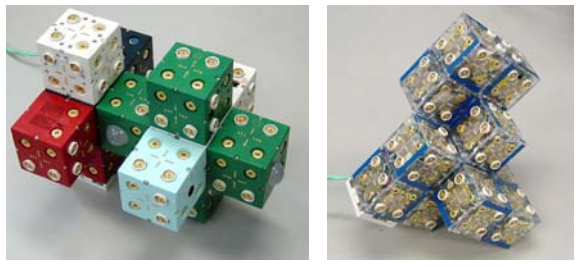
\includegraphics[width=.57\linewidth]{images/activecube}&
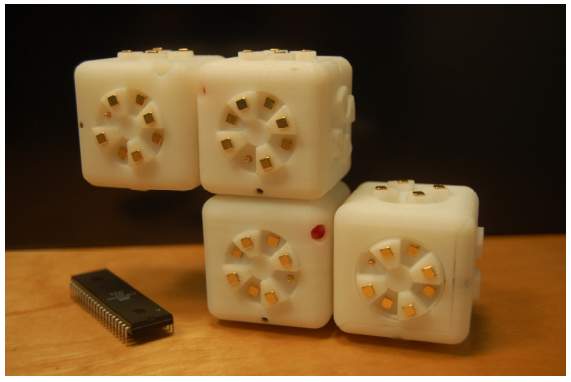
\includegraphics[width=.39\linewidth]{images/roblocks}
\end{array}$
\end{center}
\caption{Left: The ActiveCube system. Right: The Roblocks system.}
\label{fig:activecube}
\end{figure}

Related contributions focus more on the cognitive processes involved when
exploring embodied interfaces with children. Research on supporting creative
problem solving with children\cite{Bevans:2011:SCC:1979742.1979838}, arguing for
a kindergarten-influenced approach to creative thinking
\cite{Resnick:2007:IRN:1254960.1254961}, embodied approaches to analyzing
children's interactions with smart objects\cite{Antle:2009:THE:1520340.1520612},
as well as the embodied design of interfaces for introducing mathematical
concepts to kids\cite{Abrahamson:2011:TED:1999030.1999031} have shown a great
degree of correlation between physical interaction and learning in children.


\begin{figure}[ht]
\begin{center}$
\begin{array}{cc}
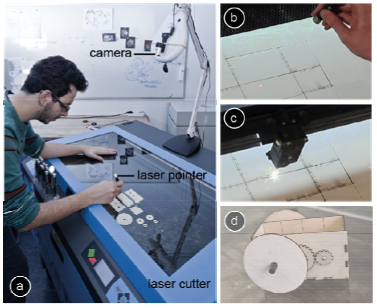
\includegraphics[width=.40\linewidth]{images/interactiveLaser}&
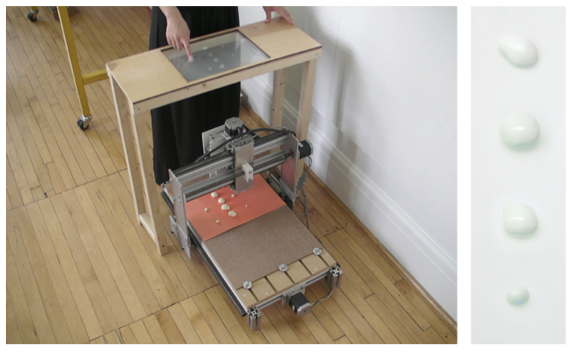
\includegraphics[width=.54\linewidth]{images/interactiveFab}
\end{array}$
\end{center}
\caption{Examples of interactive fabrication interfaces: Constructable (left)
allows users to control a laser cutter with a set of physical tools as opposed
to a pre-defined design file. Shaper (right), and interactive fabrication tool
using expanding polyurethane foam.}
\label{fig:kidcad}
\end{figure}



\begin{figure}[ht]
\begin{center}$
\begin{array}{cc}
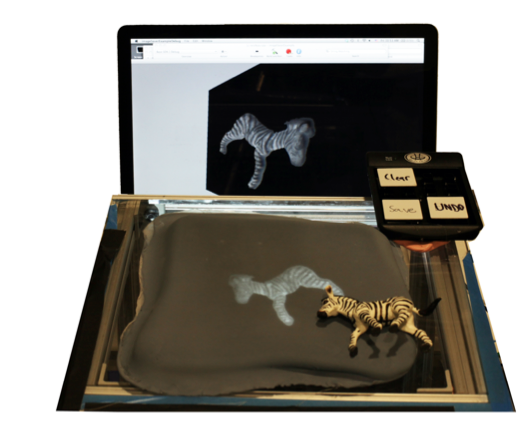
\includegraphics[width=.45\linewidth]{images/kidcad}&
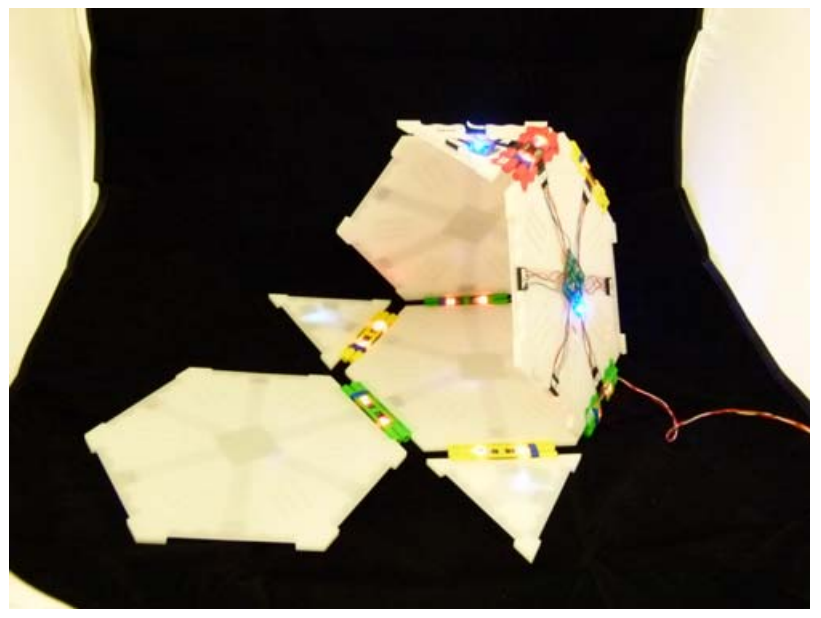
\includegraphics[width=.45\linewidth]{images/easigami}
\end{array}$
\end{center}
\caption{Left: The KidCAD interface showing a model Zebra and its 2.5D
impression on screen.
Right: The Easigami system, showing a series of connected polygonal faces with
smart-hinges and embedded electronics.}
\label{fig:kidcad}
\end{figure}

Yet so far, there have been few attempts to design embodied interfaces for
children that specifically address the growing presence and availability of
digital fabrication tools.
KidCAD\cite{Follmer:2012:KDR:2207676.2208403}, a deformable pad that captures
the 2.5D geometry of depressions made on the underside of the surface, was a
very promising idea in that it allowed very young children to take small objects
from their surroundings (or their hands) and `stamp' them into the pad - an
intuitive and satisfying experience. Unfortunately, the authors intentions to be
able to output the geometry to 3D printers has not yet manifested.
Easigami\cite{Huang:2012:EVC:2148131.2148143} is a set of interchangeable and
interlocking polyhedral faces with smart `hinges' that can reproduce the
morphology of a set of connected faces while connected to a computer. In
contrast, Easigami \emph{is} able to export this morphology to a
stereolithography file ready for 3D printing. There are several other interfaces
that deal with `interactive fabrication'\cite{Willis:2010:IFN:1935701.1935716};
devices that manipulate materials interactively based on various input from a
user, such as controlling a laser cutter with a laser pointer (instead of
through a CAD program)\cite{Mueller:2012:ICI:2380116.2380191}, or a wearable
device that takes in a CAD file and provides haptic feedback to make the
physical creation of the device by hand easier, even for a
non-fabricator\cite{Zoran:2013:FFD:2470654.2481361}.
These projects, as well as several others that deal specifically with digital
fabrication for laser
cutting\cite{Johnson:2012:SMS:2212776.2212390}\cite{Willis:2010:SSB:1709886.1709890},
are examples of the subset of tangible interfaces to which this work belongs -
namely, those concerned with providing a means to engage with digital
fabrication technologies in a more intuitive, embodied fashion. However, with
the exception of KidCAD and Easigami these designs are not made with children in
mind, nor do they cover the range of possibilities for child-friendly input
devices that focus on 3D-printing. Thus we argue that there is room for
exploration in this area, as well as a lineage that suggests meaningful results
may follow from the incorporation of tangible interfaces with embodied design.



% from IDC 2011
There are several strands of research that have strongly influenced the design
(and motivation) for the UCube. Perhaps the most fundamental of these is in the
area of "embodied mathematics"� that is, the notion that mathematical thinking
and learning are affected by, and perhaps grounded in, metaphors derived from
bodily experience. The most thorough and discursive (though largely theoretical)
discussion of these ideas is in the foundational text by Lakoff and Nu�ez [18]:
the authors discuss physically- derived metaphors that underlie such essential
mathematical ideas as numbers, operations, and sets. Such notions of embodied
mathematics have�even before the Lakoff/Nu�ez text�played a role in discussions
of the development or instruction of mathematical ideas. The link between
physical experience and mathematical growth was a strong element, for instance,
in Montessori's work (see, e.g., [15]); much of the motivation behind
traditional mathematical "manipulatives" such as number rods and balance beams
can also be traced to this intellectual tradition. More recently, theoretical
discussions of embodied cognition have given rise to fine-grained observations
of the connections between bodily activity and mathematical learning:
Goldin-Meadow [13], for instance, describes a fascinating line of research in
which children's nonverbal gestures appear to both reflect and, in some cases,
anticipate their verbal understanding of concepts such as conservation and
"inverse operations".
Pedagogical research in embodied mathematics has, moreover, proceeded
hand-in-hand with the development of desktop, embedded, or portable
technological artifacts to support the link between bodily actions and
mathematical conceptualization. Papert's discussions of the Logo computer
language [27] reveal this connection early in the history of children's
computing: Papert discussed, for example, the way in which the program for a
Logo circle resonated with children's bodily understanding of moving in a
circular path. More recently, Nemirovsky et al. [25] describe the use of a
computer-based motion detector system to assist children in the development of
intuitions behind graphing; Howison et al. [17] used a device based on a Wii
remote to assess children's understanding of ratio (the children attempt to move
their arms in a manner illustrating a target ratio); Bakker et al. [2] created a
collection of handheld objects ("MoSo Tangibles") with embedded sensors to help
children learn about musical ideas via hand motions such as waving, squeezing
(pressing hands together), and shaking up and down, among others; Mickelson and
Ju [24] use sophisticated video and projection equipment as the basis of
activities through which children can learn about mathematical ideas (e.g.,
symmetry, rotation angles) via large- scale physical movements.
The development of the UCube follows within this tradition, in that the device
was created to enable children to specify and identify three-dimensional shapes
by hand motions (instead of, by contrast, using symbolic commands directed at a
two-dimensional screen display). At the same time, the UCube is not simply a
device for mathematical instruction, but is more generally a tool for
mathematical design. As noted at the outset of this paper, the intent of the
UCube is to enable youngsters not only to learn about but also to build
mathematical shapes.
Specifically, we see the device as part of a larger, burgeoning "technological
ecosystem" around the activity of three- dimensional printing. The first section
of this paper noted several prominent researchers who argue for the
democratization of this technology, and for its applications to education.
Indeed, exciting early work has been done in applying 3D printing to education
in fields such as architecture [4], solid geometry [16], and mechanical design
[20]. The UCube is designed so that it can be employed by younger
students�younger, for instance, than the typical (undergraduate-age)
architecture student. At the same time, we see no reason at all why the device
could not be used by adult or professional-level students�particularly if (as we
anticipate) the device and software are made more expressive or powerful in
future iterations.
It should also be noted, along these lines, that our early pilot test experience
suggests a potentially fruitful use for the UCube as an assessment device for
children's spatial cognition. (The young subject who suggested that it could be
made into a "puzzle game" is anticipating our thoughts here!) A researcher
could, for instance, give children a pattern of lights and ask them to match
that pattern to one of a set of physical or pictorial solid representations; or
one might ask children to recreate a variety of physical solids (such as a
plastic prism or tetrahedron) by selecting the appropriate set of lights, and
note their development and difficulties in doing so. By using the UCube as an
experimental device in this fashion, one can position this work as part of a
tradition (dating back at least to Piaget [28]) in understanding spatial
thinking and its development (cf. also [26] for a more recent treatment of the
subject).
\chapter{Evaluation}
\label{evaluation}

This section is devoted to the description and discussion of three separate user
studies with the devices discussed in Chapter 2. Two studies were performed with
the original UCube device (one more informal than the other), while a longer,
more detailed study involved both the SnapCAD and PopCAD systems. We present the
procedure, results, and basic observations of each study in this chapter, and
discuss the results more thoroughly in the next chapter.

\section{UCube Pilot}
\subsection{Procedure}

Early in 2011, we conducted an initial (and informal) pilot test of the UCube
with a group of 12-14 year old middle school children. Fourteen participants,
consisting of five girls and nine boys, were divided into six groups (five
groups of two, one group of four). Participants were asked to model a sequence
of five shapes of increasing complexity using the UCube along with the companion
software. The target shapes were displayed on one half of a computer screen,
while the UCube software showing the live model was displayed on the other half (
as in \ref{fig:ucube_test1}).
The first shape that participants were asked to model was a straight vertical
line; after this, the requested shapes were a diagonal line, a cube, a
triangular prism, and finally an irregular polyhedral object. No shape required
more than four towers to complete, and shapes were always presented in the same
order.

\begin{figure}[!ht]
\begin{center}$
\begin{array}{cc}
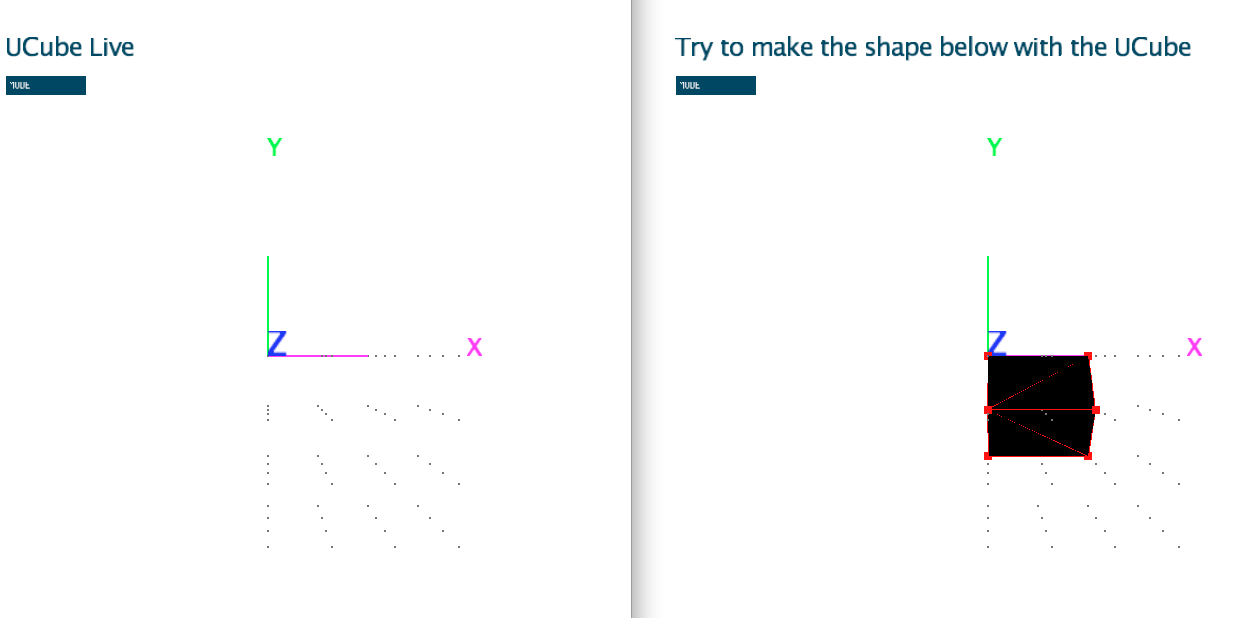
\includegraphics[width=.8\linewidth]{images/ucubescreentest}
\end{array}$
\end{center}
\caption{A screenshot of the testing setup, with the live output from the UCube
on the right and the target shape on the left.}
\label{fig:ucube_test1}
\end{figure}

Participants were instructed to place the tower on the board (but not shown
how), and were told that the software model could be rotated and filled in using
the keyboard and mouse, should that help them complete the task. The
participants were not given any hints as to how to complete the shapes and were
not told when they had the correct configuration (they had to indicate their
belief that the model was done). Participants were also instructed to ``think
aloud'' about their actions. The main purpose of the pilot study was to get an
initial impression of how the UCube would act as an accessible 3D modeling
tool - how well it could help ``3D novices'' overcome the ``2D bottleneck''.

\subsection{Results and Observations} 
Of the six groups who participated, four groups successfully modeled all five
shapes, one group ran out of time after three shapes, and one group finished one
shape, for a total of 24 of 30 possible shapes, or 80\%. Sessions lasted between
17 and 30 minutes.
A variety of problem-solving strategies were observed during testing, as the
participants tended to treat the exercise as a sort of puzzle to be solved.
Simple methods equivalent to ``try and see'' were common, and seemed to serve as
a base point from which to draw conclusions about the relationship between the
3D model and 2D on-screen representation (e.g. ``No, not there, up one''). More
sophisticated strategies were also observed: ``deconstructing'' more complex
shapes into smaller, easier-to-model shapes (e.g. thinking of one side of a cube
as a square) was observed from several groups. Another popular technique was to
systematically match the on-screen perspective from the live model with the
shape they were attempting to model (e.g. ``Okay, first let's do the top view,
and then go from the side''). By orienting the two models similarly,
participants were able to make more accurate modeling decisions as well as check
their model against the on-screen shape. Counting distance in terms of spaces on
the board, between switches, or between dots on the screen was also a very
common technique of reasoning about and describing position. For example, by
counting that two vertices of a shape were separated by ``two dots over and one
down'' on the screen, subjects were able to count the distance out on the
physical UCube board. A few of the more mathematically-advanced participants
used terms such as ``axis'' and ``origin'' to orient themselves and describe
various positions on the board to their partners.
Another revealing observation in the pilot study was that, in the few instances
of mechanical failure (certain switches not lighting up, towers not plugging in
properly, or points not showing up on screen) the participants were still able
(with a high degree of certainty) to complete the assigned tasks. This appears
to indicate that, as opposed to arbitrarily moving the towers around until the
two sides of the computer screen looked the same, participants had formed a more
substantial mental model of the relationship between the UCube interface and the
2D representations on the screen. That opens the possibility that by performing
the embodied interactions necessary to operate the UCube, participants had
actually strengthened their understanding of how 3-dimensional space is
typically represented on a 2D screen. Although a small, informal study on its
own, this finding would strengthen the argument for using the UCube in an
educational setting to improve understanding of 3D space, as well as providing a
gateway for youngsters to move on to more complex modeling software.
While the variety of problem-solving techniques we witnessed is a testament to
the participants' ingenuity, it is also indicative of the fact that parts of the
UCube are not immediately intuitive. While none of the participants had trouble
understanding how to place the towers on the platform, the positions of the
towers and switches had to be reasoned out explicitly. It was common for groups
to clear the board of any poles when starting a new shape, even in cases where
an overlap of points or tower positions existed. Although most groups completed
all the shapes (or ran out of time), there were some expressions along the way
of the difficulty of the task (e.g. ``This is hard'', or ``This is like a
puzzle''). This indicates that design changes can be made in future iterations
to help clarify the correspondence between positions on the UCube platform and
the on-screen representation; for example, labeling the both the physical and
software grid with a simple alphanumeric system.
Despite these drawbacks as well as the inherent limitations of the UCube design,
these early results indicate a promising ability of youngsters to effectively
engage with the UCube interface. In fact, despite various levels of success in
completing the assigned tasks, the vast majority of participants exhibited a
high level of engagement with the UCube. For example, although the group that
completed only one shape seemed unmotivated to attempt to model the other
shapes, they continued to play with the interface and observe the results, even
stating ``this is fun'' and ``I like the switches''. Participants also saw
potential uses for the UCube outside of the specific exercise we assigned.
Comments (unsolicited) included, ``you should use this to teach geometry'' and
``you could make this a puzzle game''. At the very least, these early results
indicate that the majority of participants were able to take a 2-dimensional
representation on the screen and model its 3-dimensional equivalent using the
UCube, a very encouraging result in our eyes, prompting refinement of
the UCube software and hardware as well as further user study, as we explain
below.

\section{Further UCube Study}

Early in 2012, we conducted another user study of the UCube with a group of
11-13 year olds. The group consisted of ten participants, eight boys and two
girls, from a local middle school multimedia class. Every participant was
individually led through two separate exercises (outlined below) using the
UCube.

\subsection{Procedure: Modeling}
Participants were handed a 3D-printed shape (modeled and printed from the UCube)
and were instructed to attempt to model the shape using the UCube. The
participant was initially allowed to hold the shape for approximately 10
seconds, after which they would hand the shape back to the facilitator and
attempt to model the shape from memory. Participants were instructed that they
may ask to hold the shape again, at which point they were allowed to hold it
throughout the duration of the modeling task. Additionally, users were
instructed that they had the option to skip a shape and return to it at a later
point in the exercise.
The five physical shapes presented were: a cube, a tetrahedron, a diamond, a
``house'' (a cube with a pyramid on top), and a complex irregular polyhedron.
The models were presented to the user starting with the cube (as this was deemed
to be the most basic shape with regard to modeling complexity). To avoid an
ordering bias, we randomized the presentation sequence of the next four shapes
using an online random order generator. If, after skipping a shape and returning
to it, the participant was still having difficulty, we offered them the
opportunity to attempt modeling the shape with the help of the UCube software,
the effects of which are discussed in the results section. Participants were
given a total of 25 minutes for the modeling exercise. We recorded, but did not
limit the modeling time per shape, only the total time for all five shapes.

\subsection{Procedure: Matching}
Participants were instructed to face away from the UCube while the facilitator
modeled a set of lights on the UCube corresponding to one shape among a set of
physical models laid out on the table next to the UCube.
Once the lights on the UCube were set up, the participant was instructed to turn
around, and indicate which physical object they thought the set of lights on the
UCube corresponded to.
There were nine physical models presented on the table, and consisted of a cube,
a tetrahedron, the ``house'' shape, a diamond, a triangular prism, an elongated
hexagon, a parallelogram, a trapezoid, and an irregular polyhedron (see
\ref{fig:ucube_shapes} for a picture of all the models). The shapes were always
presented on the table in the same order and orientation to avoid discrepancies
in perception or association.
Of the nine shapes, the participants were asked to match five of them (the cube,
the triangular prism, the parallelogram, the elongated hexagon, and the
trapezoid). Thus, only the cube was presented in both the matching and modeling
exercises. As with the modeling exercise, the cube was presented first, with the
remaining four shapes presented in a computer-generated randomized order.
Participants were given a total of ten minutes for the matching exercise,
corresponding to two minutes per shape, and were instructed to think aloud
during the process.

\begin{figure}[!ht]
\begin{center}$
\begin{array}{cc}
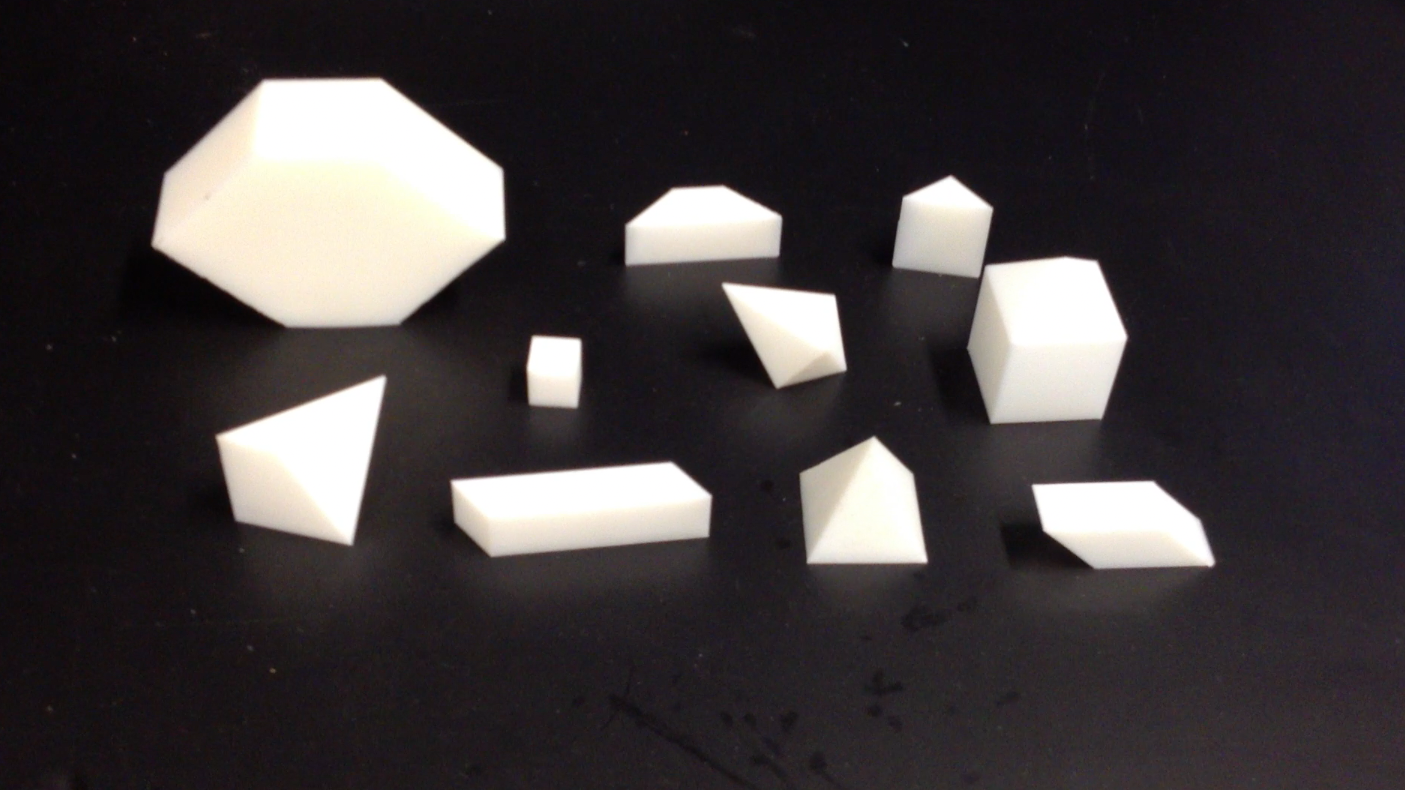
\includegraphics[width=.8\linewidth]{images/ucube_shapes}
\end{array}$
\end{center}
\caption{The nine models used during the user study:
a diamond, trapezoid, parallelogram, cube, elongated hexagon, irregular 
polyhedron, triangular prism, tetrahedron, house.}
\label{fig:ucube_shapes}
\end{figure}


\subsection{Results} 
While many established forms of 3D modeling systems can be confounding and
operationally too complex for a child to navigate, the UCube was positively
received and system instruction was accomplished with just a minor introduction
and demonstration (system instruction and demonstration lasted approximately 2-3
minutes). We found this first instance of system comprehension to offer some
validation that the UCube worked well as a user-friendly 3D modeling device.
This section will detail the outcome of both the modeling and matching tasks
performed.

\subsubsection{Exercise 1: Modeling} 
Modeling occurred under three conditions:recreate the object from memory,
construction of the object while it was in the participant�s possession, and
modeling the shape with the help of the UCube software. Overall, 21 of 50 shapes
were completed from memory, 12 of 50 were completed while holding the shape, and
a further 8 of 50 were completed with the aid of the UCube software, for a total
of 41 out of 50 shapes modeled successfully (82\%). Of the nine missed shapes,
seven were of the same shape, the complex polyhedron. The remaining two misses
were from the same participant, who ran out of time before completion.
Of the ten participants, eight were able to recreate the cube from memory,
whereas only four were able to recreate the diamond and the tetrahedron from
memory. Half of the participants constructed the house from memory, and no
participants were able to complete the irregular polyhedron from memory.
However, once shown the software the majority of the participants found the
modeling task significantly easier to perform. The irregular polyhedron was by
far the hardest shape and was only able to be completed by three of the ten
participants either after continued possession of the shape or using the
software.

\begin{figure}[!ht]
\begin{center}$
\begin{array}{cc}
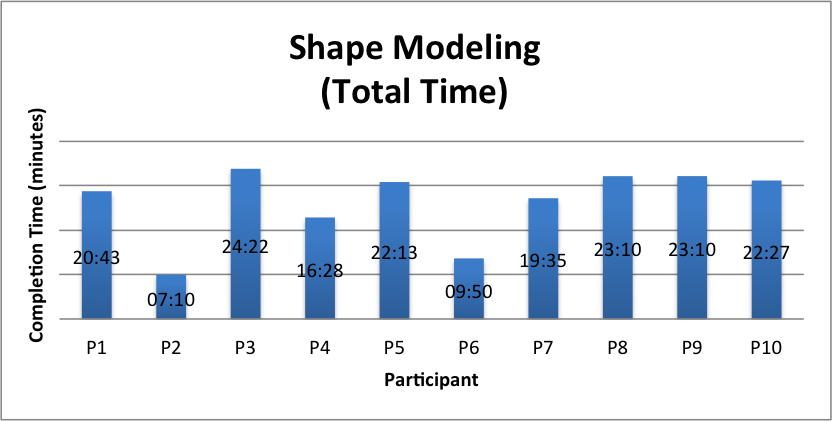
\includegraphics[width=.47\linewidth, height=1.75in]{images/modeling1}&
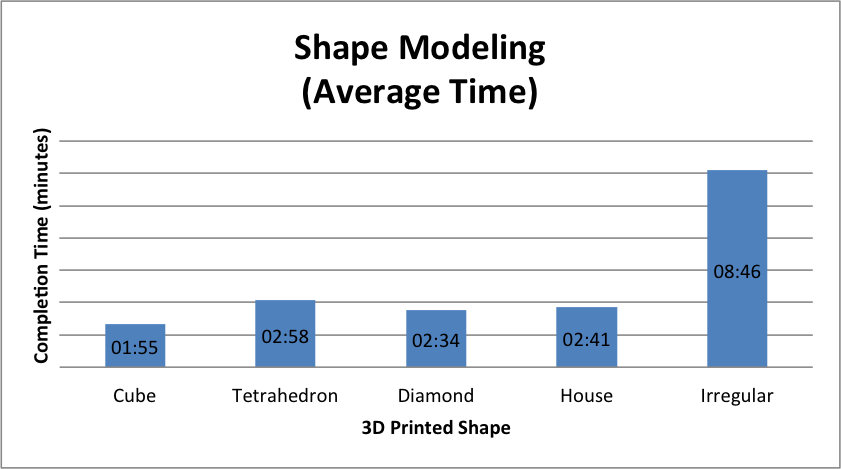
\includegraphics[width=.47\linewidth, height=1.75in]{images/modeling2}
\end{array}$
\end{center}
\caption{Results of the modeling task, showing total modeling time spent per
participant (left) and average modeling time spent per shape across
participants (right).}
\label{fig:modeling}
\end{figure}


The graphs in Figure \ref{fig:modeling} represent the total completion times per
participant (on the left) and average time per shape (right). Two exceptional
completion times were observed, where participants finished modeling all the
shapes in under 10 minutes. However, the majority of participants finished the
task in the 19-25 minute range. Only one of the participants ran out of time.
Once participants had been introduced to the software, 9 of 10 of participants
were able to complete all but the irregular polyhedron. It is interesting to
note that of the 10 participants, the child that had the most difficult time
modeling, the lowest shape completion rate, and the longest completion time
during the matching exercise was the youngest participant.


\subsubsection{Exercise 2: Matching} 
Out of 50 matching tasks (five per participant), all but three tasks were
completed in 20 seconds or less. \ref{fig:matching} displays the total time
spent on the matching task per participant (left) and the average completion
times for each shape (right).
No participant selected the wrong shape (a few preliminary ``mis-selections''
were made that the participants quickly corrected), and all participants
completed the task in well under the allotted 10 minutes. The lack of errors in
the matching task is highly encouraging as a basis from which to reason about
youngsters' abilities to perceive and reason about convex hulls as a set of lit
vertices in space, meaning that this kind of 3D modeling interface might be
applied to other domains (e.g., as a cognitive assessment tool, a puzzle game,
etc.) with some optimism.

\begin{figure}[!ht]
\begin{center}$
\begin{array}{cc}
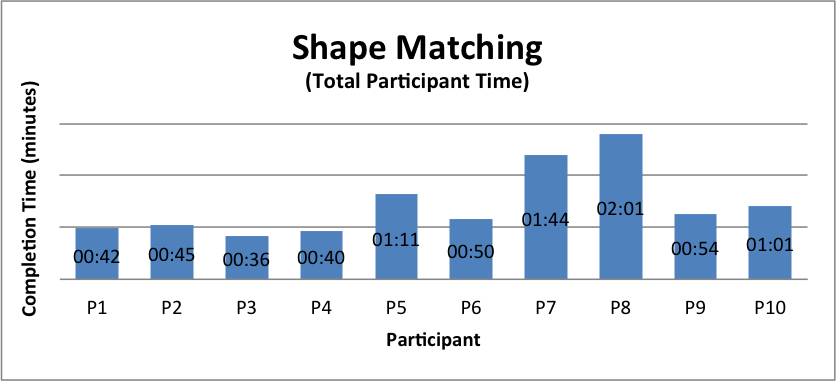
\includegraphics[width=.47\linewidth, height=1.75in]{images/matching1}&
\includegraphics[width=.47\linewidth, height=1.75in]{images/matching2}
\end{array}$
\end{center}
\caption{Results of the matching task, showing total time spent per
participant (left) and average time spent per shape across
participants (right).}
\label{fig:matching}
\end{figure}


\subsection{Results and Observations} 
Modeling trends as well as distinct modeling behaviors were documented in the
process. Common observations included building from the ground up (lowest
vertices first), building in the orientation that the object had been presented
in, not clearing the poles/lights from the UCube before starting to model a new
shape, and modeling a shape by breaking it up into discrete parts (e.g. a
participant building a house would commonly build a cube first and then add on a
vertex to the top; a participant constructing the diamond might combine two
opposite facing triangles.).

\begin{figure}[!ht] \begin{center}$
\begin{array}{cc}
\includegraphics[width=.4\linewidth]{images/idc3}&
\includegraphics[width=.5\linewidth]{images/ucube1_user}
\end{array}$
\end{center}
\caption{(Left: A participant modeling with the UCube, using a strategy of
placing the physical model on top of the UCube while modeling, as well as using both hands
simultaneously to manipulate the towers. Right: A user pointing at the software
representation of the shape with one hand, while manipulating the UCube
interface with the other hand.}
\label{fig:user_placedModel}
\end{figure}

Unique behaviors were exhibited in the modeling process as well, reflecting a
type of user specific construction-based problem solving. One participant used
their arm to connect the red lights of the UCube for shape definition. A few
participants oriented the object differently than how it had been
presented�typically this occurred for the modeling of those objects with a
pyramidal apex (tetrahedron, house, diamond). Apex formation was perhaps one of
the most difficult concepts for most participants to grasp, as it required them
to strategically align the base on a 3x3 grid so there was a middle plug for
them to create the apex. If participants were fixated on designing from a 4x4
grid then there was no center plug for them to create a midpoint. Some
participants ended up building an oblong polyhedron as opposed to a cube, or an
oblique polyhedron as opposed to an equilateral tetrahedron. Other observed
behaviors included a participant who modeled shapes by turning on lights for an
entire shape edge, as opposed to just the corners and a participant who built
shapes that were floating, as opposed to resting on the base of the UCube.
There were also some notable behaviors regarding physical and gestural actions
of the participants. Many participants modeled with both hands simultaneously,
placing towers and flipping switches without a clear preference for a dominant
hand. Participants would often gesture with their arms following an arc in
parallel with a face of the object they were currently modeling. This ``tracing''
behavior was also noticed when participants were holding a physical model and
tracing a side of the object with their fingertip, often while rotating the
object with the other hand. Finally, during object possession phase three
participants actually placed the 3D object on top of the UCube in the modeling
space while they reasoned out the construction (see
\ref{fig:user_placedModel} for an example). These gestural and ``embodied''
interactions with the UCube, combined with a high degree of modeling success
spurred us not only to create a more robust and expressive system (called -
SnapCAD - as detailed in Chapter 2), but to attempt to tease out the
relationships between modeling on these kinds of devices and the gestures and
speech produced when subjects were explaining their strategy in using the
devices. This eventually led to a comparative study using two new devices, two
new modeling modes, and introducing metrics to analyze some of the ``embodied''
aspects hinted at above.



\section{SnapCAD and PopCAD}

%- see
%http://silccenter.org/index.php/testsainstruments#MRT for the instruments, see
%http://www.spatialintelligence.org/publications_pdfs/Ehrlich\%20Levine\%20\%20Goldin-Meadow\%20\%282006\%29.pdf

Starting in early 2014 we conducted a study using both the SnapCAD and PopCAD
devices with a group of 11-18 year olds at a local drop-in enrichment program
that focuses on children from under-served and low socioeconomic communities.
Twenty participants enrolled in the study, consisting of 12 boys and 8 girls (no
one responded with other, although it was an option). We collected some basic
demographic information, including age, race, grade level, 3D modeling
experience, 3D printing experience, computer ownership and use, interest in
engineering, and how difficult they thought classes in school were. Parental
consent was obtained (and child assent given) for each subject in the study.

To present a snapshot of the demographic findings, then: the participants were
primarily of Latino or Hispanic descent, but also included those of
African-American, American-Indian, Asian, and Caucasian descent. Grade levels
ranged from 6th-12th, with an overall average of 7.9 (8.33 for boys, 7.75 for
the girls). Average age was 14 years, 1 month, 20 days (14 years, 6 months for
boys, 13 years, 7 months for girls). 16 of 20 participants had a computer at
home. Describing their comfort level using a computer on a scale from 1 to 10
(10 being most comfortable), the participants averaged 7.9 (8 for boys, 7.75 for
girls), with no scores below a 5. Of the participants who had a computer at home
(all but two of the subjects), two reported using it only a few times a year,
five used it a few times per month, four used it a few times per week, and five
reported using the computer everyday. Only three of the participants had any
experience with 3D modeling software. Interestingly, only two of the
participants had never heard of 3D printing before enrolling in the study, but
none of them had ever designed or printed anything using a 3D printer. When
asked about their interest in engineering, only seven children (all boys) stated
they were definitely interested. However, only two kids (both girls) stated that
they were definitely not. The rest (11 kids) stated that they were either
``maybe'' interested, or ``not sure''. When asked how difficult they felt school
classes were, six responded ``easy for me'', 10 said `somewhat easy for me', and
four responded ``somewhat hard for me'' (no one responded ``hard for me'').

\subsection{Procedure}

The study ran for seven weeks total, comprising several stages, the first being
a pre-assessment of spatial reasoning skills. The spatial reasoning assessment was
done using the ``Children's Mental Transformation Task'' developed by Susan
Levine (\cite{ehrlich2006importance} p.1260-1261). In the task, participants are
shown two pieces of paper, side-by-side. One piece shows a 2D geometric shape,
split apart and rotated in one of several different ways. All shapes were
symmetrical either horizontally or vertically (or both), and thus split along
either a vertical or horizontal line of symmetry. Shapes were translated in one of four
different ways: (a) translated perpendicular to the line of symmetry (direct
translation), (b) translated and then moved diagonally apart (diagonal
translation), (c) rotated 45 degrees outward from the line of symmetry (direct
rotation), or (d) rotated and then moved diagonally apart (diagonal rotation).
The other piece of paper contained the geometric shape, recombined correctly,
along with three incorrect choices. In the study we conducted, participants were
given two sets of 10 shapes, one set as a pre-assessment before doing any
modeling, and another (completely different) set of 10 after completing the
entire study, as a post-assessment. Figure \ref{spatialTest} shows an example
instrument, with the four possible translations.

\begin{figure}[!ht]
\begin{center}
\includegraphics[width=.5\linewidth]{images/SpatialTestArray}
\end{center}
\caption{An example problem from the spatial reasoning exercise. The figure at
the top shows the choice array of four shapes, where the lower left figure is
the correct option. Examples (a) through (d) show the four different types of
translations found in the exercises - direct translation, diagonal translation,
direct rotation, and diagonal rotation.}
\label{spatialTest}
\end{figure}


After the pre-assessment, participants were split into two groups of 10 students
each - the selection alternated evenly based solely on order of participation -
with group A modeling first on the PopCAD and group B modeling first on the
SnapCAD (as described in Chapter 2). Each session begins with a brief ($\approx$
one minute) introduction to the device, during which the participant is told how
to operate the device, but not what any of the software buttons do, and given
free time to become comfortable with the interface. Participants were encouraged
to explore both the interface, and the buttons in the software that control the
three primary modeling modes (convex hull, path, minimal spanning tree).

Once the subject indicates that they are ready to move on, we move into a series
of three modeling exercises that explore each of the aforementioned modes. The
basic operation and a brief explanation of each mode were given to the
participants as an introduction to each mode. Four 3D-printed models
representative of each mode were presented to the user in an order judged to be
from least complex to most complex (and thus was the same for each user), for a
total of 12 modeling tasks across the three modes. 24 models were used - one set
of 12 was used across every user's first session (independent of device), with a
remaining 12 models used in every user's second session. Figure \ref{3dModel} shows
the two sets of models side-by-side.

\begin{figure}[!ht]
\begin{center}$
\begin{array}{cc}
\includegraphics[width=.47\linewidth]{images/round1shapes}&
\includegraphics[width=.47\linewidth]{images/round2shapes}
\end{array}$
\end{center}
\caption{The two groups of 12 3D printed models used in the first session
(left) and second session (right). Each row is a different modeling mode (back
= convex hull, middle = path, and front = minimal spanning tree). The shapes
were presented in order from left to right as pictured above.}
\label{3dModel}
\end{figure}


The tasks that follow are the same for each device:

Tasks 1-3: Convex Hull Modeling, Path Modeling, Minimal Spanning Tree Modeling

Before each set of modeling tasks, the participant will be given a brief demo of
how each modeling mode interprets the points from the device.  The user will
then be presented with a series of four (4) plastic, 3D-printed models that were
modeled on the device using the current modeling mode. For each of these shapes,
the participant will attempt to recreate the shape using the modeling abilities
of the device and the software. The user will be instructed to indicate when
they believe they have successfully recreated the shape, as well as to think
aloud about their modeling process. The time to completion (of lack thereof),
completion code, observational notes, and video shall be recorded. If the user
indicates success, they shall be asked to explain their modeling strategy for
the purpose of logging gesture and speech data.

Task 4: Freehand Modeling

After the modeling tasks are complete, participants are invited to ``freestyle''
model an object of their choosing, using any of the three modeling modes. By
asking participants to think aloud about their intentions and thinking processes
during this exercise, we hope that a deeper understanding may be gained of the
strengths and weaknesses of the system, as well as the thought processes and
engagement of the users in attempting to model a specific model of their own
choosing. These saved models are analyzed, based on which mode was used to
create them, complexity (based on number of points used), and whether the shape
was `exploratory' or `intentional' (i.e., was the end artifact a result of sort
of happy accident, or the result of intentional process to create a specific
model).


For the first three modeling tasks (but not the freestyle modeling), time to
completion (or request to move on) is recorded, along with an outcome code. The
outcome is coded according to a set of conditions detailed below in table
\ref{modelingError}, and was developed upon analysis of the recorded video, in
an attempt to fit the sorts of repeated behaviors that were in fact observed.

\begin{table}[!ht]
\small
    \caption[Coding rubric used in analyzing modeling exercise outcomes.]{
	The coding used in analyzing the modeling exercise outcomes, based on
	observations from video taken during the study.}
    \begin{center}
    \begin{tabular}{| p{3.5cm} | p{1.0cm} | p{7.2cm} | } \hline
	$Category$ & $Code$ & $Definition$   \\ \hline
	Correct & C & A complete and correct modeling of the shape \\ \hline
	Error in recognition & E1 & The correct shape was modeled, but the user did not
	identify it \\ \hline 
	Error in belief & E2 & A belief that the modeled shape has been modeled
	correctly, when it has not \\ \hline 
	Error in implementation & E3 & User knew shape was incorrect, and gave a
	correct explanation \\ \hline 
	Error in strategy & E4 & Knew shape was incorrect, and did not know why or gave
	an incorrect explanation as to why \\ \hline 
	Error in proportion & EP & The general shape is correct, but the proportions in
	one or more dimensions is off (e.g. too tall, not wide enough, etc.) \\ \hline
	Incomplete & I & Participant ran out of time, gave up, or asked to move on \\
	\hline
	\end{tabular}
   \\ \rule{0mm}{5mm}
\end{center}
\label{modelingError}
\end{table}

Participants were asked to ``think aloud'' about their process, difficulties,
modeling choices, etc. In the case that the user believed they had correctly
modeled the shape (cases C and E2 in table \ref{modelingError}) they were asked
to explain their modeling strategy\footnote{Cases E1,E3,E4, and I did not
provide the grounds from which to ask about modeling strategy and so were not
recorded.}. Their explanation was videotaped and analyzed based on the coding
strategies laid out in ``The Importance of Gesture in Children's Spatial
Reasoning"(\cite{ehrlich2006importance}, p.1264), laid out in table
\ref{GcodingStrategy} below. The rationale for performing this analysis in based
in part on work by Ehrlich, Levine, and Goldin-Meadow
\cite{ehrlich2006importance}\cite{levine1999early}\cite{goldin2005hearing},
which suggests that the frequency of gesture and relationships between speech
and gesture act as a window into the learning state and performance of the
subjects.

\begin{table}[!ht]
\small
    \caption[Coding rubric for speech and gesture during user explanation of
    modeling strategy]{ The various coding strategies used in the video
    analysis of subjects' modeling strategy explanations. Borrowed and adapted
    from \cite{ehrlich2006importance}.}
    \begin{center}
    \begin{tabular}{| p{1.5cm} | p{4.2cm} | p{4.2cm} | p{4.2cm} |} \hline
	$Category$ & $Definition$ &   $Speech Examples$  & $Gesture Examples$ \\ \hline
	Movement & Any indication of movement & ``Just slide them together and then it
	looks like that'' & Miming movement with the hands\\ \hline 
	Perceptual Features & Focus on a particular feature of the model & ``Because
	there is a little bend in here and a point thing here'' & Pointing to a
	specific feature on the model \\ \hline 
	Perceptual Whole & Any indication of seeing the model as a whole & ``It looks
	like an arrow!'' & Gesture indicating inclusion of the whole shape \\ \hline
	Vague & An expression of strategy that the coder cannot decipher & ``Because I
	looked at that and I looked at the differences'' & Waving gestures above the
	computer device that do not indicate any specific strategy \\ \hline 
	Other & Any strategy not listed above & ``And here is like half of it.
	But so and two halves make a whole'' & Using the hand to form a straight line
	through the middle of the whole shape to represent the line of symmetry
	\\
	\hline
	\end{tabular}
   \\ \rule{0mm}{5mm}
\end{center}
\label{GcodingStrategy}
\end{table}


The second session is similar to the first, with the subject using the device
not used in session one, and with 12 new models. Once modeling on the second
device is completed, users will take a second spatial reasoning assessment of an
additional ten questions to help gauge if any meaningful difference in spatial
reasoning skills has occurred throughout the study. 

A slightly modified version of the software was used for the user study,
eliminating several of the functions not being evaluated for the sake of
presenting a clear interface for the users. The multiple hull modes, spline,
load, and save functions (described in Chapter 2) were eliminated, and the rest
of the graphical user interface was reorganized and streamlined. We
combined the three different .stl export buttons into a single export button
that handled all three modes, changed the order of the remaining buttons and
made them larger, and made the X,Y, and Z axis markings larger.

\subsection{Results}

This section reports on the results from our study, relaying our findings across
both sessions, genders, modeling modes, and spatial reasoning scores in an
attempt to tease out what conclusions, if any, we might make about the strengths
and weaknesses of our devices as well as how interacting with our devices
affected user's spatial reasoning abilities, 3D modeling skills, or congruence
between speech and gesture in explaining the cognitive learning state of the
user.

\subsubsection{Modeling Results}

In this section we will focus on delivering the results from the modeling
exercises - users went through two sessions, modeling 12 shapes each time (4
shapes each using convex hull, path, and minimal spanning tree modes) for a
total of 24 exercises. For each modeling task, a result code was recorded per
the rubric shown in table \ref{modelingError}. One user dropped out of the study
(user 6) before completing round one, leaving us to report on 19 users for the
first modeling session, 10 of whom started on the PopCAD and 9 of whom started
with the SnapCAD. A further three users did not complete session 2, leaving 16
users, 7 girls and 9 boys, who were split evenly over the two devices (four
each on PopCAD and SnapCAD).

% \begin{table}[!ht] 
% \small
%     \caption[Modeling Results Overview]{This table gives the subject's age,
%     gender, and number of correctly completed modeling tasks during each of the
%     two sessions.}
%     \begin{center}
%     \begin{tabular}{| c | c | c | c | c | c | c |} \hline
% 	$User$ & $Age$ & $Gender$ & $Device$ & $S1$ $Score$ & $Device$ & $S2$ 
% 	$Score$\\\hline 
% 	1 & 14 & M & Pop & 11 & Snap & 9 \\ \hline
% 	2 & 12 & F & Snap & 6 & Pop & 8 \\ \hline
% 	3 & 15 & M & Pop & 6 & Snap & 3 \\ \hline
% 	4 & 13 & M & Snap & 4 & Pop & 5 \\ \hline
% 	5 & 12 & M & Pop & 5 & Snap & 6 \\ \hline
% 	7 & 15 & M & Pop & 12 & Snap & 11 \\ \hline
% 	8 & 12 & F & Snap & 4 & Pop & 8 \\ \hline
% 	9 & 18 & M & Pop & 8 & Snap & 3 \\ \hline
% 	10 & 14 & F & Pop & 12 & Snap & 10 \\ \hline
% 	11 & 17 & M & Snap & 9 & Pop & 12 \\ \hline
% 	12 & 12 & M & Snap & 4 & Pop & 7 \\ \hline
% 	13 & 13 & M & Pop & 9 & -- & -- \\ \hline
% 	14 & 14 & M & Snap & 1 & Pop & 5 \\ \hline
% 	15 & 12 & M & Snap & 1 & -- & -- \\ \hline
% 	16 & 13 & M & Pop & 12 & -- & -- \\ \hline
% 	17 & 13 & F & Pop & 11 & Snap & 9 \\ \hline
% 	18 & 17 & F & Snap & 8 & Pop & 12 \\ \hline
% 	19 & 11 & F & Pop & 4 & Snap & 3 \\ \hline
% 	20 & 13 & F & Snap & 0 & Pop & 5 \\ \hline
% 	\end{tabular}
%    \\ \rule{0mm}{5mm}
% \end{center}
% \label{modelOverview}
% \end{table}

\begin{table}[!ht] 
%\small
    \caption[Modeling Results Overview]{An overview of the modeling task
    results, broken down into session number, gender, device, and modeling
    mode.}
    \begin{center}
    \begin{tabular}{| c | c | c | c | c | c | c | } \hline
	& $Session$ $1$ & \% & $Session$ $2$ & \% & $Total$ & \% \\\hline 
	$Overall Correct$ & 127/228 & 55.7\% & 116/192 & 60.4\% & 243/420 & 57.9\%  \\
	\hline $Girls$ & 45/84 & 53.6\% & 55/84 & 65.5\% & 100/168 & 59.5\%  \\ \hline
	$Boys$ & 82/144 & 57.6\% & 61/108 & 56.5\% & 143/252  & 56.7\%   \\ \hline
	$PopCAD$ & 90/120 & 75\% & 62/96 & 64.6\% & 152/216 & 70.4\%  \\ \hline
	$SnapCAD$ & 37/108 & 34.3\% & 54/96 & 56.3\% & 91/204 & 44.6\%  \\ \hline
	$Convex$ $Hull$ & 40/76 & 52.6\% & 38/64 & 59.3\% & 78/140 & 55.7\%  \\ \hline
	$Path$ & 48/76 & 63.2\% & 44/64 & 68.8\% & 92/140 & 65.7\%  \\ \hline
	$Tree$ & 39/76 & 51.3\% & 34/64 & 53.1\% & 73/140 & 52.1\%  \\ \hline
	\end{tabular}
   \\ \rule{0mm}{5mm}
\end{center}
\label{modelOverview}
\end{table}

Out of the 228 modeling tasks in session one, the group successfully modeled
127, or roughly 56\%. Those users who started with SnapCAD performed 37 of 108
tasks, or 34\%, while those using the PopCAD device completed 90 of 120 tasks
correctly, for a success rate of 75\%. Girls completed 45 of 84 tasks (54\%),
while boys correctly completed 82 of 144 tasks (58\%). Individual scores ranged
from 0 to 12 (perfect), with an overall overage of 6.68 correct shapes per user.
Average correct shapes per user was 4.11 for SnapCAD and 9.00 for PopCAD.

In session two, 116 of 192 (60\%) tasks were performed correctly, with SnapCAD
modelers correctly representing 54 of 96 shapes (56\%) and PopCAD modelers
completing 62 of 96 shapes, or roughly 65\%. Girls completed 55 of 84 tasks
(65\%) while boys completed 61 of 108 tasks for 56\%. Individual scores ranged
from 3 to 12 (perfect), with an average of 7.25 correct shapes overall, while
the average correct shapes per user was 6.75 for SnapCAD and 7.75 for PopCAD.


% \begin{table}[!ht] 
% \small
%     \caption[Session one modeling results per shape]{ This table shows the
%     number of correct models generated from a given shape, broken down by
%     device, gender, and average modeling time spent on the shape. Session one
%     results only.}
%     \begin{center}
%     \begin{tabular}{| c | c | c | c | c | c | c |} \hline
% 	$Shape$ & $Total$ & $PopCAD$ & $SnapCAD$ & $Average$ & $PopCAD$
% 	& $SnapCAD$ \\
% 	 & $Number Correct$ & $Only$ & $Only$ & $Modeling Time$ & $Only$ & $Only$
% 	 \\\hline 
% 	 Convex Hull 1 & 8 & 7 & 1 & 6:33 & 5:25 & 7:49 \\ \hline 
% 	 Convex Hull 2 & 13 & 9 & 4 & 4:34 & 3:03 & 6:15 \\ \hline 
% 	 Convex Hull 3 & 8 & 7 & 1 & 5:29 & 4:33 & 6:32 \\ \hline 
% 	 Convex Hull 4 & 11 & 7 & 4 & 4:52 & 4:31 & 5:14 \\ \hline 
% 	 Path 1 & 17 & 10 & 7 & 2:08 & 1:22 & 3:00 \\ \hline 
% 	 Path 2 & 14 & 9 & 5 & 4:39 & 3:24 & 6:02 \\ \hline 
% 	 Path 3 & 8 & 6 & 2 & 6:21 & 4:52 & 8:00 \\ \hline 
% 	 Path 4 & 9 & 7 & 2 & 4:12 & 1:56 & 6:43 \\ \hline 
% 	 Tree 1 & 12 & 8 & 4 & 2:10 & 1:10 & 3:17 \\ \hline 
% 	 Tree 2 & 8 & 6 & 2 & 2:25 & 1:08 & 3:51 \\ \hline 
% 	 Tree 3 & 8 & 5 & 3 & 3:11 & 1:29 & 5:04 \\ \hline 
% 	 Tree 4 & 11 & 8 & 3 & 4:24 & 3:12 & 5:43 \\ \hline
% 	 \em{Total} & 127 & 90 & 37 & 4:15 & 3:00 & 5:38 \\ \hline
% 	\end{tabular}
%    \\ \rule{0mm}{5mm}
% \end{center}
% \label{codingStrategy}
% \end{table}

The two bar graphs in \ref{ModelingTimes} show the average modeling times broken
out over device and gender (on the top) and modeling mode (on the bottom).
Modeling times were recorded from the time the user was handed the shape until
they indicated either that (a) they believed the model to be complete, or (b)
they gave up, wished to move on, or thought they were as close as they were
going to get (though they knew their model to be incorrect). 

\begin{figure}[!ht]
\begin{center}$
\begin{array}{cc}
\includegraphics[width=.55\linewidth]{images/modelTimesPerDevice} \\
\includegraphics[width=.55\linewidth]{images/modelTimesPerMode}
\end{array}$
\end{center}
\caption{The average recorded modeling times for each session, broken out (on
top) by device and gender, and (on the bottom) by modeling mode.}
\label{ModelingTimes}
\end{figure}

We can easily pick out a few trends from these two graphs: average modeling
session time went down significantly in the second session, regardless of device
or gender, although boys took less time in both sessions, and the PopCAD seemed
to take less time overall in each session than modeling on the SnapCAD (although
interestingly, the SnapCAD modelers in the second round improved on their times
from modeling on the PopCAD in the first round). When examining mode types, we
see a similar trend of significantly decreasing modeling times in the convex
hull and path modes, but curiously, not in the tree mode where times improved in
the second session by only a few seconds. While the minimal spanning tree mode
took subjects the least amount of time (of the three modes) in session one, the
improvement in both convex hull and path modeling times left the spanning tree
with slowest overall and average modeling times in session two.
Seeing as the minimal spanning tree mode posted the lowest percentage of correct
shapes in both rounds (and thus overall), we might expect the ranking we
observed in round two, where average modeling times corresponded with the
overall percentage of correct shapes. It seems plausible that mastery of the
tree mode is slower to arrive than either the convex hull or path modes, and
therefore one extra session produced more dramatic results in the other modes
(convex hull and path modeling both improved by almost 7\% in session two,
minimal spanning tree by less than 2\%). 



% Given the massive development (both cognitively and physically) that occurs
% between the age extremes in our subject population (11 to 18), it would be
% tempting (and even logical) to assume that the older subjects would perform much
% better on the modeling tasks than their younger counterparts. However, we found
% a very modest correlation ($r = .39, p < .15$) between age and the number of
% correctly modeled shapes, suggesting it may play less of a role then we would
% have suspected. It is possible that the statistics are slightly misleading here
% - the subject population was weighted toward the younger end of the spectrum:
% the average age was 13.8, while median age was 13.5, and the mode was 12 years
% old. Meaning the few older participants would have had to perform impossibly
% brilliantly (i.e., higher than the highest possible score) for a strong age to
% performance correlation to show up.

% \begin{table}[!ht] 
% \small
%     \caption[Modeling Times per user (overall)]{Modeling times per user over
%     all modeling exercises in session 1.}
%     \begin{center}
%     \begin{tabular}{| c | c | c | c | c | c | c | } \hline 
%     $Mode$ & $Combined$ & $Number$ & $PopCAD$ & $SnapCAD$ & $Girls$ &
%     $Boys$ \\
%     &  $Average Time$  & $Correct$ & $Only$     & $Only$ & & \\ \hline     
%      Convex Hull &  21:30:21 & 40 / 76 &  30 & 10 & 14 & 26\\ \hline 
%      Path &  17:21:57 & 48 / 76 &  33 & 15 & 17 & 31 \\ \hline 
%      Minimal Spanning Tree &  12:11:52 & 39 / 76 &  27 & 12 & 14 & 25 \\ \hline 
%      Overall &  51:04:10 & 127 / 228 &  90 & 37 & 45 & 82 \\ \hline 
% 	\end{tabular}
%    \\ \rule{0mm}{5mm}
% \end{center}
% \label{modelingTimes}
% \end{table}


\subsubsection{Mental Transformation Task Results}

Subjects were given two sets of 10 mental transformation problems, as discussed
previously in the procedure section. The first set was given before the first
modeling session, as a sort of pre-assessment. The second set was given after
the second modeling session as a post-test. We recorded performance data by
session and by user, and present the results in Figure \ref{mttbreakdown} broken
out by the type of symmetry represented in the shape (unilateral or bilateral)
and the type of translation or rotation performed on the shape (direct or
diagonal translation, direction or diagonal rotation), meaning that each shape
had both a symmetry type and a translation type.


\begin{figure}[!ht]
\begin{center}
\includegraphics[width=.9\linewidth]{images/MTTshapeChar}
\end{center}
\caption{A view of the Mental Transformation Task results, broken out by
symmetry type (B = bilateral, U = unilateral) and rotation or translation type
performed on the shape being transformed.}
\label{mttbreakdown}
\end{figure}

Overall, subjects performed very well on the Mental Transformation Task,
correctly responding to 614 of 720 questions (a little over 85\%). Performance
was remarkably equal across genders, with girls correct on 256 of 300 (85.3\%)
and boys on 358 of 420 (85.2\%). Accordingly, we found no sigificant difference
in gendered responses across any symmetry or translation type - girls and boys
succeeded and struggled on the same sorts of tasks. Bilateral symmetry was
significantly easier than unilateral, with over 90\% of bilateral tasks and only
78\% of unilateral tasks performed correctly. Rotation was more difficult than
translation, and diagonal transformations were more problematic than direct
ones. Hence, diagonal rotations scored the lowest (75\%), followed by direct
rotations (82\%), diagonal translations (91\%), and direct translations (93\%).

% \begin{table}[!ht] 
% \small
%     \caption[Mental Transformation Task by Shape Profile and
%     Translation Type]{Mental Transformation Task by Shape Profile and
%     Translation Type}
%     \begin{center}
%     \begin{tabular}{| c | c | c | c | c | c | c | c | } \hline 
%     $  $ & $Bilateral$ & $Unilateral$ & $Direct$ & $Direct$ & $Diagonal$ &
%     $Diagonal$ & $Total$ \\
%     & $Symmetry$ & $Symmetry$ & $Translation$ & $Rotation$ &
%     $Translation$ & $Rotation$ & $Correct$ \\ \hline
%     $Session 1$ & 109/120 & 57/80 & 54/60 & 34/40 & 56/60 & 22/40 & 166/200 \\
%     \hline 
%     $Girls$ & 43/48 & 23/32 & 22/24 & 13/16 & 23/24 & 8/16 & 66/80 \\ \hline
%     $ Boys $ & 66/72 & 34/48 & 32/36 & 21/24 & 33/36 & 14/24 & 100/120 \\ \hline
%     $ $ &  &  &  &  &  &  & \\ \hline
%     $Session 2$ & 72/80 & 69/80 & 31/32 & 39/48 & 28/32 & 43/48 & 141/160 \\
%     \hline 
%     $Girls$ & 32/35 & 30/35 & 13/14 & 18/21 & 12/14 & 19/21 & 62/70 \\ \hline
%     $Boys$ & 42/45 & 39/45 & 18/18 & 21/17 & 16/18 & 24/27 & 79/90 \\ \hline
%     $ $ &  &  &  &  &  &  & \\ \hline
%     $Combined$ & 181/200 & 126/160 & 85/92 & 73/88 & 84/92 & 65/88 & 307/360 \\
%     \hline 
%     $Girls$ & 75/83 & 53/67 & 35/38 & 31/37 & 35/38  & 27/37 & 256/300 \\ \hline
%     $Boys$ & 108/117 & 73/93 & 50/54 & 42/51 & 49/54 & 38/51 & 360/420 \\ \hline
% 	\end{tabular}
%    \\ \rule{0mm}{5mm}
% \end{center}
% \label{MTTbyShape}
% \end{table}

% \begin{table}[!ht] 
% \tiny
%     \caption[Mental Transformation Task
%     Performance Per User]{Mental Transformation Task Performance Per User.}
%     \begin{center}
%     \begin{tabular}{| c | c | c | c | c | c | c | c | c | c | c | c | c | c | c
%     | c | c | c | c | c | c |} \hline 
%     $User$ & 1 & 2 & 3 & 4 & 5 & 6 & 7 & 8 & 9 & 10 & 11 & 12 & 13 & 14 & 15 &
%     16 & 17 & 18 & 19 & 20 \\ \hline
%     $Set$ $1$ & 7 & 10 & 8 & 7 & 9 & 8 & 10 & 9 & 9 & 7 & 9 & 8 & 10 & 9 & 6 &
%     8 & 10 & 8 & 7 & 7 \\\hline 
%     $Set$ $2$ & 9 & 9 & 10 & 6 & 10 & - & 10 & 10 & 10 & 10 & 9 & 9 & - & 6 &
%     - & - & 10 & 8 & 5 & 10 \\ \hline 
%     $Total$ & 16 & 19 & 18  & 13  & 19 & - & 20  & 19 & 19  & 17 & 18  & 17  & - 
%     & 15 & - & - & 20 & 16 & 12 & 17\\ \hline 
%     $Change$ & +2 & -1 & +2 & -1 & +1 & - & 0 & +1 & +1 & +3 & 0 & +1 & - &
%     -3 & - & - & 0 & 0 & -2 & +3 \\ \hline
% 	\end{tabular}
%    \\ \rule{0mm}{5mm}
% \end{center}
% \label{MTTperUser}
% \end{table}

\begin{figure}[!ht]
\begin{center}
\includegraphics[width=.9\linewidth]{images/MTTPerformance}
\end{center}
\caption{Mental Transformation Task results, broken down by session and by
user.}
\label{MTTPerformance}
\end{figure}

Figure \ref{MTTPerformance} shows the Mental Transformation Task results broken
down into sessions by user. We observed a +7 net improvement in the second round
among the 16 users who participated in both sessions. Both girls and boys
improved in the second session, though girls improved by a greater percentage
when compared to boys - from 82.3\% to 88.6\% while boys improved from 83.3\% to
87.7\%, a 2\% greater improvement among girls. Four users did worse on the
second set of tasks, four did the same, and 8 improved; the greatest change in
both directions was +/- 3. There was a weak correlation between improvement
between sessions (or lack thereof) and modeling performance overall ($r = .20, p
< .5$), but a weak negative correlation between improvement on the Mental
Transformation Task and improvement in modeling score from session 1 to session
2 ($r=-.20, p <.5$), suggesting that the \emph{change} between sessions on the
spatial reasoning test and modeling performance are mildly related, if at all.

\subsubsection{Speech and Gesture Coding Results}

During the modeling exercises, if a subject believed (whether correctly or not)
that they had successfully modeled a shape, the facilitator asked the subject to
describe the modeling strategy they used to arrive at their answer. During these
explanations, video recordings were analyzed for five types of speech and
gesture behaviors: those referring to movement, to the perceptual whole of the
shape being modeled, to a perceptual feature of the shape being model, as well
as behaviors that were vague or unintelligible, and those that did not fit into
any of the above categories (labeled as ``other'' - a more detailed description
is available in the procedure section above). A given strategy was only recorded
once per modeling task, but multiple strategies per explanation occurred often and
were recorded (as was also the case in \cite{ehrlich2006importance}). The tables
below break down the numbers and types of speech and gestures observed over the
two sessions; as such, we only report on the 16 subjects who completed both
sessions.

% \begin{table}[!ht] 
% \tiny
%     \caption[Session 1 Gesture and Speech Observations]{Gesture and
%     Speech Observations over both sessions.}
%     \begin{center}
%     \begin{tabular}{| c | c | c | c | c | c | c | c | c | c | c | c | c | c | c
%     |} \hline
%     User & G.M & G.PW & G.PF & G.V & G.O & G Tot. & S.M & S.PW & S.PF & S.V &
%     S.O & S Tot. & G Tot. + & No. \\   
%     & & & & & & & & & & & & & S Tot. & Corr. \\ \hline
%     1 &4 &0 &8 &7 &0 &19 &4 &3 &7 &13 &4 &31 &50 &20 \\ \hline
%     2 &10 &1 &10 &6 &0 &27 &7 &7 &9 &6 &2 &31 &58 &14  \\ \hline
%     3 &1 &0 &9 &1 &0 &11 &4 &2 &11 &4 &0 &21 &32 &9  \\ \hline
%     4 &0 &0 &5 &9 &0 &14 &1 &7 &12 &9 &2 &31 &45 &9  \\ \hline
%     5 &6 &0 &11 &5 &0 &22 &8 &2 &11 &6 &4 &31 &53 &11  \\ \hline
%     7 &4 &0 &15 &6 &0 &25 &6 &3 &15 &2 &12 &38 &63 &23  \\ \hline
%     8 &1 &0 &2 &4 &0 &7 &1 &0 &2 &4 &0 &7 &14 &12  \\ \hline
%     9 &4 &2 &3 &10 &0 &19 &10 &6 &4 &8 &1 &29 &48 &11  \\ \hline
%     10 &10 &4 &19 &8 &2 &43 &5 &9 &19 &6 &4 &43 &86 &22  \\ \hline
%     11 &11 &2 &15 &5 &1 &34 &8 &3 &16 &5 &7 &39 &73 &21  \\ \hline
%     12 &6 &0 &10 &8 &0 &24 &5 &4 &7 &10 &3 &29 &53 &11  \\ \hline
%     14 &4 &1 &8 &7 &0 &20 &6 &3 &6 &7 &4 &26 &46 &6  \\ \hline
%     17 &16 &2 &23 &6 &0 &47 &14 &12 &22 &0 &7 &55 &102 &20  \\ \hline
%     18 &12 &1 &19 &2 &0 &34 &13 &3 &22 &2 &10 &50 &84 &20  \\ \hline
%     19 &17 &0 &14 &7 &2 &40 &13 &2 &14 &16 &3 &48 &88 &7  \\ \hline
%     20 &7 &0 &9 &9 &2 &27 &2 &2 &9 &6 &7 &26 &53 &5  \\ \hline
% 	\end{tabular}
%    \\ \rule{0mm}{5mm}
% \end{center}
% \label{MTTperUser}
% \end{table}


\begin{table}[!ht] 
\small
    \caption[Gesture and Speech Observations]{Gesture and Speech
    Observations over both sessions. Numbers in this table exclude the
    totals from the three subjects who finished the first session but not the
    second. \\ G = Gesture, S = Speech, .M = Movement, .PW = Perceptual Whole,
    .PF = Perceptual Feature, .V = Vague, .O = Other.}
    \begin{center}
    \begin{tabular}{| c | c | c | c | c | c | c | c | c | c | c |} \hline
	& $Total$ & & $PopCAD$ & $SnapCAD$ & & $Girls$ & $Boys$ & & $Session$ $1$ &
	$Session$ $2$\\ \hline 
	$G.M$ &113 & &62 &51 & &73 &40 & &39 &74 \\ \hline
	$G.PW$ &13 & &8 &5 & &8 &5 & &9 & 4 \\ \hline
	$G.PF$ &180 & &102 &78 & &96 &84& &93 &87 \\ \hline
	$G.V$ &100 & &50 &50 & &42 &58& &34 & 66 \\ \hline
	$G.O$ &7 & &4 &3 & &6 &1& &4 & 3\\ \hline
	 & & & & & & & & & &\\ \hline
	$S.M$ &107 & &64 &43 & &55 &52& &46 & 61\\ \hline
	$S.PW$ &68 & &39 &29 & &35 &33& & 38& 30 \\ \hline
	$S.PF$ &186 & &103 &83 & &97 &89 & &101 &85 \\ \hline
	$S.V$ &104 & &55 &49 & &40 &64 & &32 &72 \\ \hline
	$S.O$ &70 & &35 &35 & &33 &37 & & 18 & 52 \\ \hline
	 & & & & & & & & & & \\ \hline
	$Gesture$ &413 & &226 &187 & &225 &188& &179 & 234 \\ \hline
	$Speech$ &535 & &296 &239 & &260 &275 & & 235& 300\\ \hline
	$Combined$ &948 & &522 &426 & &485 &463& & 414& 534 \\ \hline
	\end{tabular}
   \\ \rule{0mm}{5mm}
\end{center}
\label{MTTperUser}
\end{table}

Table \ref{MTTperUser} shows the total number of gesture and speech types we
recorded, as well as how they were split between each devices, genders, and
sessions. The most common gesture and speech types (by a
significant margin) were about specific perceptual features of the models, those
relating to movement came next, followed closely by vague gestures and speech.
The other two categories, perceptual whole and ``other'' strategies, were barely
represented in gesture - they were far more common in speech, but still ranked
as the least frequently recorded. Many users explained their modeling strategy
by doing a ``step-by-step'' recounting of their process that referred at each
step to the part of the shape they were modeling at that point. For example, it
was common for a subject to point to a segment of the model and say (for
instance), ``and then I put a point here, for this part\ldots'', generating
perceptual feature scores in both gesture and speech for nearly every
explanation they gave. Movement was often explained along the same lines
(though less frequently), often with subject using specific words that
indicate motion (e.g. ``then I move over here'', ``I had to go up here, then
follow the path back down again'') while simultaneously motioning along the
directions they were indicating.

Interestingly, even without accounting for the difference in number of subjects,
girls ``out-gestured'' the boys overall (225 to 188), and in every category
\emph{except} for vague gestures, where boys were vague in describing their
strategies 24 more times over the course of the study. Speech types were more
gender-balanced, with the final tally being 260 for girls and 275 for boys,
however seeing as boys had more participants in both sessions of the study, the
speech-per-participant count actually favors the girls as well. The PopCAD
interface produced more gestures (226 to 187) and speech (296 to 239) than the
SnapCAD, a finding mitigated somewhat by the fact that users modeled so poorly
on the SnapCAD in the first round and therefore did not arrive at a point where
a modeling strategy could be explained. If we isolate the second round only,
where the performance breakdown was much more even (62 to 54 in favor of
PopCAD), then SnapCAD actually produced more gestures (124 to 110) and more
speech elements (159 to 141). 

Perhaps the most curious data from Table \ref{MTTperUser} is the big increase in
both gesture and speech from round 1 to round 2 of the study. Even with three
less participants in round 2, overall instances of gestures increased from round
1 by 55 (179 to 234, a 76\% increase), and speech instances increased by 65 (235
to 300, a 78\% increase), yet the overall modeling performance only increased by
5\% in round 2. A bit of a closer look at the types of gesture and speech gives
a plausible explanation: in both gesture and speech, the number of \emph{vague}
indications rose dramatically (+32 for gesture, +40 for speech), while the
number of perceptual feature indications dropped in both cases (-6 for gesture,
-16 for speech). If we look at Figures \ref{gesturebreakdown} and
\ref{speechbreakdown} these numbers start to make more sense.

\begin{figure}[!ht]
\begin{center}
\includegraphics[width=.85\linewidth]{images/GesturePerfBreakdown}
\end{center}
\caption{A plot of the five types of gestures we coded (movement, perceptual
whole, perceptual feature, vague, and other) over the number of correctly
modeled shapes. The slope of the lines indicate the strength of correlation
between each gesture type and overall modeling performance.}
\label{gesturebreakdown}
\end{figure}

Figure \ref{gesturebreakdown} shows a plot of the number and kind of gestures
produced by a user over the number of shapes they modeled correctly over the two
rounds of the study.\footnote{Data from the three users who dropped out of the
study has been omitted from this graph as well as Figure \ref{speechbreakdown}}
The lines associated with each scatter plot shows the strength of the
correlation between instances of that gesture type and modeling performance; the
steeper the positive slope, the higher the positive correlation and vice versa.
As we can see from the graph, three of the conditions have positive slopes
(perceptual feature, movement, and perceptual whole), while two have negative
slopes (vague and other). By far the strongest positive correlation\footnote{All
correlation calculations were done using Pearson's Correlation Coeffcient.} is
between perceptual feature gesturing and modeling performance ($r = .61, p <
.025$), while vague gesturing has a weak negative correlation ($r = -.22, p <
.5$). Going back to our earlier table, then, the sharp uptick in vague gestures
and mild decline of perceptual features may help to explain why such an increase
in gesturing did not result in a similar upswing in modeling performance.


\begin{figure}[!ht]
\begin{center}
\includegraphics[width=.85\linewidth]{images/SpeechBreakdown}
\end{center}
\caption{A plot of the five types of speech we coded (movement, perceptual
whole, perceptual feature, vague, and other) over the number of correctly
modeled shapes. The slope of the lines indicate the strength of correlation
between each speech type and overall modeling performance.}
\label{speechbreakdown}
\end{figure}

One might expect that correlation patterns would be similar between gestures and
speech of the same type (e.g. instances of movement in gesture would be as
correlated to modeling performance as instances of movement in speech), and
while we did find some similarities, some surprising differences appeared as
well. Speaking about perceptual features was (as with gesturing) the most highly
correlated type to modeling success ($r = .58, p < .025$), but where gestures
marked as ``other'' had a very weak negative correlation, ``other'' categories
of speech were second most \emph{highly} correlated with modeling aptitude ($r
=. 56, p < .025$) - nearly as much as utterances on perceptual features. Part of
this explanation lies in the frequency discrepancy between ``other'' gestures,
of which there were only seven, and ``other'' speech utterances, of which there
were ten times more (70). The other (pardon the pun) part of the explanation
lies in the fact that we have many more words with specific meanings than
gestures that are precisely defined, so (for example) explanations referring to
looking at the software itself (e.g., ``I looked at the screen and it looked
like it.''), or reasoning about the nature of how the mode works (e.g., ``Since
it was path I knew it would work.''), or internal operations (e.g., ``I just
look at it and see it''), are harder to perceive in gesture. A possible relation
to the potential for specificity in speech lies in the stronger observed
negative correlation between modeling ability and speech marked as vague ($r=
-.41, p < .25$), compared to gestures marked as vague ($r=-.22, p < .5$),
indicating (perhaps) that a failure to speak specifically (given more abundant
options) is more harmful than a similar failure when gesturing.


\subsection{Observations}

A few notes on the above findings are worth making here. Broadly speaking, the
study indicated many positive outcomes: overall modeling ability went up while
average modeling time went down, the participants improved on every modeling
mode in the second session, there was a net positive performance on the second
mental transformation task when compared with the first, and participants were
generally engaged by the experience, which for most subjects was their first
computer-based 3D modeling experience. However, even though no user saw the same
device or shape twice, it is as yet unclear how much of the improvement might be
contributed to a ``practice effect''. Due to the ``drop-in'' nature of the user
study environment, the time between each single participants' sessions varied,
based on their attendance and availability (i.e., in some cases users had
homework or other activities to finish).

We observed some moderate correlations between types of speech and gesture and
modeling success, though not necessarily the kinds of correlations we might have
expected based on prior related studies. Nor were speech and gesture correlated
to modeling acumen in the same ways - some types of gesture were less effective
than their corresponding spoken elements, and vice versa. In some cases, the
results were observed were counter-intuitive - such as the anomaly in average
modeling times of subjects when using the minimal spanning tree mode, the fact
that boys performed worse during the second modeling session while girls
performed much better, and that some subjects performed worse on the second
mental transformation task, even though they were arguably ``primed'' by going
through the modeling exercises beforehand. Also unexpected is the sharp decline
in performance on the PopCAD device in the second session - over 10\% -
especially after such a high percentage in the first round and given more
``experienced'' users in the second session. Equally surprising, given a rather
unimpressive first round performance, is the sharp increase in modeling success
on the SnapCAD in the second round (a jump of 12\%), so much so that when
coupled with the decline in PopCAD performance, we may wonder on the possible
disparity between the groups in ``inherent'' ability for these kinds of tasks.
Another possibility is of course that the order in which subject encouter the
devices is more important than we had originally surmised - perhaps the users
who started with PopCAD did better on the SnapCAD (and overall) \emph{because}
they started with PopCAD. We examine these, as well as the relevance of age and
shape complexity on modeling ability, along with a deeper discussion of results
across all three studies in the following chapter.






% Given the massive development (both cognitively and physically) that occurs
% between the age extremes in our subject population (11 to 18), it would be
% tempting (and even logical) to assume that the older subjects would perform much
% better on the modeling tasks than their younger counterparts. However, we found
% a very modest correlation ($r = .39, p < .15$) between age and the number of
% correctly modeled shapes, suggesting it may play less of a role then we would
% have suspected. It is possible that the statistics are slightly misleading here
% - the subject population was weighted toward the younger end of the spectrum:
% the average age was 13.8, while median age was 13.5, and the mode was 12 years
% old. Meaning the few older participants would have had to perform impossibly
% brilliantly (i.e., higher than the highest possible score) for a strong age to
% performance correlation to show up.
% 
% Popcad first avg age: 14
% snapcad first : 13.75
% 
% 
% In order to attempt to judge each shape's complexity, we sought out a
% previously-defined set of criteria by which to judge ``complexity''. As it turns
% out, there is a long and thorough discussion of complexity in relation to
% \emph{two-dimensional} shapes, starting seemingly with Fred Attneave and Malcolm
% Arnoult\cite{attneave1956quantitative}\cite{attneave1957physical} in the mid
% 1950's, who define methods of generating random two-dimensional shapes and
% examine their physical characteristics in relation to their judged complexity.
% As it turns out (in \cite{attneave1957physical} as well as others' follow-up
% work) the ``Number of Turns'' in the shape was responsible for significant
% amount (nearly 80\% in Attneave's study) of the preceived complexity of a shape.
% ``Number of Turns'' is defined as, ``the number of maxima (regardless of sign)
% in one cycle of the function relating curvature to distance along the contour.
% This function is a series of spikes for any angular shape, and a step-function
% for any curved shape\ldots'' (see pp. 226 of the aforementioned article).
% Symmetry, angular variability, and squared perimeter over area also had some
% affect.
% 
% However, as it seems unclear to us how one might adapt a ``Number of Turns''
% rating to a true \emph{three dimensional} model. Although many studies claim to
% have studied complexity in relation to mental transformation tasks, starting
% with Shepard and Metzler\cite{shepard1971mental}, who instead used perspective
% line drawings, not actual physical models. This had an advantage for the types
% of mental rotation tasks they were performing (recognition of matching pairs),
% and similarly set off a wave of studies using the same (or similar) ``faux 3D''
% stimuli\cite{metzler1974transformational}\cite{shepard1988mental}\cite{vandenberg1978mental}.
% 
% All of which leads us to determine (as best we way) the complexity of the shapes
% we presented in the study, as a way of teasing out any correlation between
% complexity and performance. In lieu of attempting an exact number of turns
% estimate, we included three criteria: (a) the minimum number of lights necessary
% to guarantee the correct shape,\footnote{In minimal spanning tree models where a
% placement of lights results in several possible correct formations, only one of
% which is the desired shape, we add points necessary to ``force'' the correct
% representation.} (b) the number of faces (for convex hull models only), the
% number of line segments (for path models only), or the number of distinct
% branches (for tree models only), and (c) a symmetry score based on number of
% lines of symmetry, from 3 (indicating asymmetry) to 0 (indicating 3 or more
% lines of symmetry). The scaling for symmetry comes from the belief that
% indicators (a) and (b) above are more closely aligned with Attneave's ``number
% of turns'' metric (being highly correlated to perceived difficulty), while
% symmetry was much less correlated to complexity (although symmetry did still
% play a part), so we made the scale as low as possible so that it would weigh
% less on the overall complexity score of a model. So, for example, a regular
% octahedron would have 6 points, 8 faces, and a 0 symmetry score for an overall
% difficulty score of 14. The complexity score of each shape is shown in
% \ref{modelComplexity} next to the number of times it was modeled correctly. The
% shapes in each session were of course different, but are labeled the same in
% this table, indicating the order in which they were presented.
% 
% 
% 
% \begin{table}[!ht] 
% \small
%     \caption[Complexity of Models and Modeling Performance]{Complexity of Models
%     and Modeling Performance (CH = Convex Hull, P = Path, T = Minimal Spanning
%     Tree)}
%     \begin{center}
%     \begin{tabular}{| c | c | c | c | c | c | c | c | c | c | c | c | c | }
%     \hline $ $ & CH1 & CH2 & CH3 & CH4 & P1 & P2 & P3 & P4 & T1 & T2 & T3 & T4 \\
%    	\hline
%    	$Session$ $1$ & & & & & & & & & & & &  \\ \hline
%    	$Complexity$ $Score$ & 14 & 19 & 19 & 19 & 7 & 18 & 20 & 24 & 9 & 13 & 17 &
%    	17 \\ \hline 
%    	$Performance$ of 19 & 8 & 13 & 8 & 11 & 17 & 14 & 8 & 9 & 12 & 8 & 8 & 11 \\
%    	\hline 
%    	$Session$ $2$ & & & & & & & & & & & & \\ \hline
%    	$Complexity$ $Score$ & 12 & 20 & 15 & 13 & 14 & 14 & 18 & 17 & 21 & 17 & 16
%    	& 25 \\ \hline 
%    	$Performance$ of 16 & 7 & 9 & 11 & 11 & 11 & 13 & 8 & 12 & 7 & 11 & 7 & 9 \\
%    	\hline
%    	
% 	\end{tabular}
%    \\ \rule{0mm}{5mm}
% \end{center}
% \label{modelComplexity}
% \end{table}
% 
% 
% One might expect to see a strong negative correlation between a given model's
% complexity score and the number of subjects who were able to model it correctly,
% however the observed correlation (using Pearson's correlation coefficient) was
% only moderate: $r = -0.41, p < .05$ over both sessions.
% 
% 
% Levine and Goldin-Meadow's research found the highest correlation occurred
% between the number of movement gestures produced over the number of correct
% answers given. 
% 
% 
% 
% The process of modeling is different than that of shape matching - modeling is
% by necessity a series of step-by-step, piecemeal operations, whereby in a mental
% transformation task, it is possible both to look at specific features of a shape
% as well as receive a more holistic mental image of the shape at hand. This may
% account in part for the relative lack of correlation between movement gestures
% and performance when compared to \cite{ehrlich2006importance}. Instead, we found
% a much higher correlation between gestures relating to perceptual features of
% the shape and modeling performance. One might argue that by looking at
% perceptual features of the shape, one is mentally ``breaking apart'' the shape
% into discrete chunks that can be turned into an order of operations for
% successfully modeling a shape.

\chapter{Vision}
\label{vision}
\chapter{Future Work}
\label{future}
%%%%%%%%%   then the Bibliography, if any   %%%%%%%%%
\bibliographystyle{plain}	% or "siam", or "alpha", etc.
\nocite{*}		% list all refs in database, cited or not
\bibliography{refs}		% Bib database in "refs.bib"

%%%%%%%%%   then the Appendices, if any   %%%%%%%%%
\appendix
\chapter{Conference Posters and Visualizations}	% *NOT* \OnePageChapter


\begin{figure}[!ht]
\begin{center}
\includegraphics[width=.62\linewidth]{images/UCube_dam_poster}
\end{center}
\caption{The poster used at the presentation of the UCube at the Denver Art
Museum.}
\label{dam}
\end{figure}



\begin{figure}[!ht]
\begin{center}
\includegraphics[width=.9\linewidth]{images/FabLearn_Poster}
\end{center}
\caption{The poster presented at the 2013 FabLearn conference at Stanford
University, in support of a short paper by the same name\cite{leducembodied}.}
\label{fablearn}
\end{figure}






% \paragraph{About appendices:}
% 	Each appendix follow the same page-numbering rules
% 	as a regular chapter; the first page of a
% 	(multi-page) appendix is not numbered.
% 	By the way, the following are supposedly
% 	authentic answers to English GCSE exams!
% 
% 
% \begin{enumerate}
% 
% \item
% The Greeks were a highly sculptured people, and without
% them we wouldn't have history. The Greeks also had myths.
% A myth is a female moth.
% 
% \item
% Actually, Homer was not written by Homer but by another
% man of that name.
% 
% \item
% Socrates was a famous Greek teacher who went around
% giving people advice. They killed him. Socrates died from an
% overdose of wedlock. After his death, his career suffered a
% dramatic decline.
% 
% \item
% Julius Caesar extinguished himself on the battlefields
% of Gaul. The Ides of March murdered him because they thought
% he was going to be made king. Dying, he gasped out: Tee hee,
% Brutus.
% 
% \item
% Nero was a cruel tyranny who would torture his subjects
% by playing the fiddle to them.
% 
% \item
% In midevil times most people were alliterate. The
% greatest writer of the futile ages was Chaucer, who
% wrote many poems and verses and also wrote literature.
% 
% \item
% Another story was William Tell, who shot an arrow
% through an apple while standing on his sons head.
% 
% \item
% Writing at the same time as Shakespeare was Miguel
% Cervantes. He wrote Donkey Hote. The next great author
% was John Milton. Milton wrote Paradise Lost. Then his
% wife died and he wrote Paradise Regained.
% 
% \item
% During the Renaissance America began. Christopher
% Columbus was a great navigator who discovered America while
% cursing about the Atlantic. His ships were called the Nina,
% the Pinta, and the Santa Fe.
% 
% \item
% Gravity was invented by Issac Walton. It is chiefly
% noticeable in the autumn when the apples are falling
% off the trees.
% 
% \item
% Johann Bach wrote a great many musical compositions and
% had a large number of children. In between he practiced on
% an old spinster which he kept up in his attic. Bach died
% from 1750 to the present. Bach was the most famous composer
% in the world and so was Handel. Handel was half German
% half Italian and half English. He was very large.
% 
% \item
% Soon the Constitution of the United States was adopted
% to secure domestic hostility. Under the constitution the
% people enjoyed the right to keep bare arms.
% 
% \item
% The sun never set on the British Empire because the
% British Empire is In the East and the sun sets in the West.
% 
% \item
% Louis Pasteur discovered a cure for rabbis. Charles
% Darwin was a naturalist who wrote the Organ of the Species.
% Madman Curie discovered radio. And Karl Marx became one of
% the Marx brothers.
% 
% \end{enumerate}

\chapter{Ode to Spot}	\OnePageChapter         % ONE PAGE!

\noindent\paragraph{(Data, Stardate 1403827)}
(A one-page chapter --- page must be numbered!)
Throughout the ages, from Keats to Giorchamo, poets have
composed ``odes'' to individuals who have had a profound effect
upon their lives.  In keeping with that tradition
I have written my next poem \ldots in honor of my cat.
I call it\ldots{}Ode\ldots{}to Spot.
(Shot of Geordi and Worf in audience,
looking mystified at each other.)


\begin{quotation}
\noindent Felus cattus, is your taxonomic nomenclature \\
an endothermic quadruped, carnivorous by nature? \\
Your visual, olfactory, and auditory senses \\
contribute to your hunting skills, and natural defenses. \\
I find myself intrigued by your sub-vocal oscillations, \\
a singular development of cat communications \\
that obviates your basic hedonistic predilection \\
for a rhythmic stroking of your fur to demonstrate affection. \\
A tail is quite essential for your acrobatic talents; \\
you would not be so agile if you lacked its counterbalance. \\
And when not being utilized to aid in locomotion, \\
It often serves to illustrate the state of your emotion.
\end{quotation}


\noindent(Commander Riker begins to applaud, until a
glance from Counselor Troi brings him to a halt.)
Commander Riker, you have anticipated my denouement.
However, the sentiment is appreciated.  I will continue.


\begin{quotation}
\noindent O Spot, the complex levels of behavior you display \\
connote a fairly well-developed cognitive array. \\
And though you are not sentient, Spot, and do not comprehend \\
I nonetheless consider you a true and valued friend.
\end{quotation}



\end{document}

